%% @Author: Ahmad Ben Taleb
%  @Date:   2026
%% @Class:  PFE ITBS V3.

\documentclass[a4paper, oneside, 12pt, final]{extreport}
\usepackage{graphicx}

\usepackage{titlesec}
\titlespacing*{\chapter}{0pt}{-30pt}{20pt}

\parindent 0cm
\usepackage{makeidx}
\usepackage{tcolorbox}
\usepackage[table]{xcolor}
\usepackage{url}
\usepackage{graphicx}
\usepackage[space]{grffile}
\usepackage{float}        % Required for [H] figure/table placement
\usepackage{placeins}     % FloatBarrier command
\usepackage{caption}      % Better caption formatting
\usepackage{tabularx}     % Flexible table columns
\usepackage{booktabs}     % Professional table rules
\usepackage{tikz}
\usetikzlibrary{positioning}
\usepackage{amssymb}
\usepackage{microtype}      % Better line breaking (TeXPage)
\emergencystretch=2em       % Reduce overfull hbox warnings
\makeindex
\graphicspath{{./figures/}{./logo/}{./}{../figures/}{../logo/}}  % TeXPage: figures live in ./figures/
%\usepackage[french]{babel}
\usepackage[lined,boxed,commentsnumbered, english, ruled,vlined,linesnumbered]{algorithm2e}
\usepackage{amsthm}
\newtheorem{theorem}{Theorem}[chapter]
\newtheorem{definition}{Definition}[chapter]
\newtheorem{exemple}{Example}[chapter]


%\usepackage[nottoc]{tocbibind}
%\addcontentsline{toc}{section}{References}

\providecommand{\keywords}[1]{\textbf{\textit{Mots clés---}} #1}
\providecommand{\keywordss}[1]{\textbf{\textit{Keywords---}} #1}

\usepackage{etoolbox}
%\makeatletter
%\patchcmd{\thebibliography}{%
%  \chapter*{\bibname}\@mkboth{\MakeUppercase\bibname}%{\MakeUppercase\bibname}}{%
%  \section{References}}{}{}
%\makeatother



\usepackage[nottoc]{tocbibind}

\textwidth 18cm
\textheight 24cm
\topmargin -0.5cm
\oddsidemargin -1cm

% set font encoding for PDFLaTeX or XeLaTeX
\usepackage{ifxetex}
\ifxetex
  \usepackage{fontspec}
\else
  \usepackage[T1]{fontenc}
  \usepackage[utf8]{inputenc}
  \usepackage{lmodern}
\fi


% Enable SageTeX to run SageMath code right inside this LaTeX file.
% documentation: http://mirrors.ctan.org/macros/latex/contrib/sagetex/sagetexpackage.pdf
%\usepackage{sagetex}


\newcommand{\reportTitle} {%
  %\textsc{Graduation Project Report}
  \textsc{Projet de Fin d'\'etudes}
}

\newcommand{\reportAuthor} {%
  Ahmed ElAbed%
}

\newcommand{\reportSubject} {%
  Conception et Implémentation d'une Plateforme\\%
  Business Intelligence et Machine Learning pour la\\%
  Direction Marché Entreprises de l'ATB%
}



\newcommand{\studyDepartment} {%
  la \textit{Direction March\'{e} Entreprises} de l'\textbf{Arab Tunisian Bank (ATB)}%
}

\newcommand{\ITBS} {%
  l'\textbf{International Tunis Business School (ITBS)}%
}

%\newcommand{\codePFE} {% Reference
%  Code PFE%
%}


\newcommand{\AU} {
\centering \textbf{Année Universitaire 2024-2025}
}


\newcommand{\specialcell}[1]{%
  \begin{tabularx}{\textwidth}{@{}X@{}}#1\end{tabularx}%
}

%%%%%%%%%%%%%%%%%%%%%%%%%%%%%%%%%%%%%%%%%%%%%%%%%%%%%%%
% Add your own commands here
%%%%%%%%%%%%%%%%%%%%%%%%%%%%%%%%%%%%%%%%%%%%%%%%%%%%%%%
\newcommand{\MyCommand} {%
  Does nothing really%
}


% used in maketitle
\title{\reportSubject}
\author{\reportAuthor}

% Enable SageTeX to run SageMath code right inside this LaTeX file.
% documentation: http://mirrors.ctan.org/macros/latex/contrib/sagetex/sagetexpackage.pdf
%\usepackage{sagetex}

%\hypersetup{
%  pdftitle={\reportTitle~-~\reportSubject},%
%  pdfauthor={\reportAuthor},%
%  pdfsubject={\reportSubject},%
%  pdfkeywords={report} {internship} {pfe} {enis}
%}

\usepackage{graphics}
\usepackage{graphicx}


\usepackage[acronym,toc,section=chapter,nonumberlist]{glossaries}
\makeglossaries

\newacronym{atb}{ATB}{Arab Tunisian Bank}
\newacronym{itbs}{ITBS}{International Tunis Business School}
\newacronym{bi}{BI}{Business Intelligence}
\newacronym{etl}{ETL}{Extract, Transform, Load}
\newacronym{dwh}{DWH}{Data Warehouse}
\newacronym{kpi}{KPI}{Key Performance Indicator}
\newacronym{ml}{ML}{Machine Learning}
\newacronym{dbt}{dbt}{data build tool}
\newacronym{dag}{DAG}{Directed Acyclic Graph}
\newacronym{shap}{SHAP}{Shapley Additive exPlanations}
\newacronym{crispdm}{CRISP-DM}{Cross-Industry Standard Process for Data Mining}
\newacronym{gimsi}{GIMSI}{G\'{e}n\'{e}rer des Indicateurs de performance pour le Management Strat\'{e}gique de l'Information}
\newacronym{sme}{SME}{Small and Medium-sized Enterprises}
\newacronym{auc}{AUC}{Area Under the Curve}
\newacronym{xgboost}{XGBoost}{Extreme Gradient Boosting}
\newacronym{sql}{SQL}{Structured Query Language}
\newacronym{api}{API}{Application Programming Interface}

\pagenumbering{roman} 

\usepackage[utf8]{inputenc}
%\usepackage[french]{babel}

\begin{document}
\thispagestyle{empty}
\begin{titlepage}
\centering


\includegraphics[scale=0.16]{embleme.jpg}

\vspace{0.3cm}
{\fontsize{9pt}{11pt}\selectfont
Republic of Tunisia \\
Ministry of Higher Education and Scientific Research \\
\textbf{International Tunis Business School (ITBS)}
}

\vspace{0.5cm}

\includegraphics[scale=0.09]{logonoir.png}

\vspace{0.6cm}
{\textit{Graduation project submitted in partial fulfilment of the}}\\[0.25cm]
{\textbf{\large National Engineering Diploma in Computer Engineering \\
Specialisation: Business Intelligence}}\\[0.5cm]

\textbf{\textit{Prepared by}}\\[0.2cm]
{\Large\bfseries\scshape Ahmed ElAbed}\\[0.5cm]

\rule{0.52\textwidth}{0.4pt}\\[0.35cm]
{\large\bfseries Customer Risk Assessment and Management \\ for Enterprise Clients at Arab Tunisian Bank }\\[0.35cm]
\rule{0.52\textwidth}{0.4pt}\\[0.6cm]

\begin{minipage}{0.9\textwidth}
\begin{tabular}{@{}p{0.46\textwidth}@{\hspace{0.04\textwidth}}p{0.46\textwidth}@{}}
\textbf{Academic Supervisor:} & \textbf{Professional Supervisor:} \\[0.15cm]
Mrs Nesrine Tarhouni & Mr Mohamed Saddek Snoussi \\
\end{tabular}
\end{minipage}

\vfill
\textbf{\textit{Graduation project carried out at}}\\[0.15cm]
\textit{Corporate Banking Division --- Arab Tunisian Bank (ATB)}\\[0.25cm]

\includegraphics[scale=0.18]{atb_logo.png}\\[0.35cm]
\textbf{Academic Year 2025--2026}

\end{titlepage}

% ###############################
% # HELP COMMANDS               #
% ###############################
%
% -1 \part{part}
%  0 \chapter{chapter}
%  1 \section{section}
%  2 \subsection{subsection}
%  3 \subsubsection{subsubsection}
%  4 \paragraph{paragraph}
%  5 \subparagraph{subparagraph}


%%%%%%%%%%%%%%%%%%%%%%%%%%%%%%%%%%%%%%%%%%%%%%%%%%%%%%%
% Dédicace et Remerciements
%%%%%%%%%%%%%%%%%%%%%%%%%%%%%%%%%%%%%%%%%%%%%%%%%%%%%%%
% Nécessite : \usepackage{graphicx}, \usepackage{tcolorbox}, \usepackage{geometry} (pour marges A4, optionnel)
\thispagestyle{empty}
\noindent
\begin{tcolorbox}[colback=white, colframe=gray!80, width=\textwidth, height=0.38\textheight, sharp corners, boxrule=0.8pt]
    \centering
    
\includegraphics[width=0.4\textwidth]{logonoir.png} % Ajuste la taille si besoin
    \vspace{5cm}

    \hfill
    \begin{minipage}[b]{0.4\textwidth}
        \hrule
        \centering
        {\footnotesize Signature et cachet de l'entreprise}
    \end{minipage}
\end{tcolorbox}

\vspace{2cm}

\noindent
\begin{tcolorbox}[colback=white, colframe=gray!80, width=\textwidth, height=0.38\textheight, sharp corners, boxrule=0.8pt]
    \centering
    
\includegraphics[width=0.4\textwidth]{logonoir.png} % Ajuste la taille si besoin
    \vspace{5cm}

    \hfill
    \begin{minipage}[b]{0.4\textwidth}
        \hrule
        \centering
        {\footnotesize Signature de l'encadrant académique}
    \end{minipage}
\end{tcolorbox}

\chapter*{Dedication}
%\chapter*{D\'edicace}
%\addcontentsline{toc}{chapter}{Dedication}
\thispagestyle{empty}

\begin{center}
\itshape
I dedicate this graduation project:
\end{center}

\begin{flushright}
\begin{minipage}{0.9\textwidth}
\itshape

To my mother,\\
who never ceased to support and encourage me.\\
Whatever I achieve, I will never thank her enough for her kindness,\\
her sacrifices and her affection.\\
May God protect her.

\vspace{0.5cm}

To my father,\\
who patiently awaited this day.\\
In recognition and deep gratitude for his sacrifices and devotion.\\
May God protect him.

\vspace{0.5cm}

To my academic and professional supervisors,\\
for their guidance, trust and constant availability throughout this work.

\vspace{0.5cm}

To my family and friends,\\
for their encouragement at every stage of this journey.

\end{minipage}
\end{flushright}

\chapter*{Acknowledgment}
%\chapter*{Remerciements}
%\addcontentsline{toc}{chapter}{Thanks}
\thispagestyle{empty}

This graduation project would not have been possible without the support of many people
to whom I wish to express my sincere gratitude.

I warmly thank my academic supervisor for her availability, rigorous feedback and
methodological guidance, which helped structure this work from the problem statement
through to the final deliverables. I equally thank my professional supervisor at the
Arab Tunisian Bank for welcoming me into the Corporate Banking Division, for sharing
business expertise on customer risk and compliance, and for steering the project toward
operationally useful outcomes.

I am grateful to the teams of the Corporate Banking Division at ATB for the trust they
placed in this platform and for the exchanges that clarified real decision needs behind
the KPIs, alerts and dashboards. I also thank International Tunis Business School (ITBS)
and its teaching staff for the academic framework that made this engineering diploma
possible.

Finally, my deepest thanks go to my family and friends for their patience, encouragement
and unfailing support throughout this internship and the writing of this report.




\begin{abstract}

The present work is part of a graduation project carried out within the company \studyDepartment in order to obtain the national diploma of engineer at the \ITBS.

This project aims to design and implement a Business Intelligence and Machine Learning platform dedicated to customer risk assessment and management at the Arab Tunisian Bank (ATB). The platform was built across three successive releases. The first established a secure, role-based environment and a fully automated data orchestration engine that refreshes all banking data every night without human intervention. The second built the analytical foundation, transforming raw operational data into a structured data warehouse and delivering interactive dashboards covering customer portfolio analytics, account monitoring, and a transparent multi-pillar risk scoring system. The third introduced a predictive layer through a supervised machine learning classifier that screens customers for risk, with model tracking, explainability features, and seamless integration into the existing dashboard. The outcome is a unified decision-support platform that gives risk managers, compliance officers, and general management a shared, reliable view of their customer portfolio. \\

\keywordss{Business Intelligence, Machine Learning, Data Warehouse, Customer Risk Assessment, Apache Airflow, Streamlit, MLflow, SHAP, Banking Analytics} \\

\vspace{3cm}
\centerline{\bf Résumé}
\vspace{0.6cm}

Ce travail s'inscrit dans le cadre du projet de fin d'études réalisé au sein de \studyDepartment en vue de l'obtention du diplôme national d'ingénieur à l'\ITBS.

Ce projet a pour objectif de concevoir et de mettre en œuvre une plateforme de Business Intelligence et de Machine Learning dédiée à l'évaluation et à la gestion du risque client au sein de l'Arab Tunisian Bank (ATB). La plateforme a été livrée en trois releases successives. La première a mis en place un environnement sécurisé basé sur les rôles ainsi qu'un moteur d'orchestration entièrement automatisé qui actualise l'ensemble des données bancaires chaque nuit sans intervention humaine. La deuxième a construit la couche analytique, transformant les données opérationnelles brutes en un entrepôt de données structuré et alimentant des tableaux de bord interactifs couvrant l'analyse du portefeuille client, le suivi des comptes et un système de scoring de risque multi-piliers. La troisième a introduit une couche prédictive reposant sur un classificateur supervisé d'apprentissage automatique, accompagné d'un suivi des expériences, d'une explicabilité des prédictions et d'une intégration fluide dans le tableau de bord existant. Le résultat est une plateforme d'aide à la décision unifiée, offrant aux gestionnaires de risque, aux responsables de conformité et à la Direction Générale une vision partagée et fiable de leur portefeuille client. \\

\keywords{Business Intelligence, Machine Learning, Entrepôt de Données, Évaluation du Risque Client, Apache Airflow, Streamlit, MLflow, SHAP, Analytique Bancaire}

\end{abstract}

%%%%%%%%%%%%%%%%%%%%%%%%%%%%%%%%%%%%%%%%%%%%%%%%%%%%%%%
% Divers chapitres
%%%%%%%%%%%%%%%%%%%%%%%%%%%%%%%%%%%%%%%%%%%%%%%%%%%%%%%
\addtocontents{toc}{\protect\setcounter{tocdepth}{4}}
\tableofcontents
%\addcontentsline{toc}{chapter}{\contentsname}

\listoffigures
%\addcontentsline{toc}{chapter}{Liste des Figures}
\listoftables
%\addcontentsline{toc}{chapter}{Liste des Tableaux}
\glsaddall
\printglossaries

\cleardoublepage

\newpage
\pagenumbering{arabic}
\chapter*{General Introduction}
\label{chap:general_intorduction}
\vspace{0.5cm}

\markboth{\MakeUppercase{General Introduction}}{}%
\addcontentsline{toc}{chapter}{General Introduction}%

In today's banking environment, managing customer risk is no longer simply a matter
of intuition or experience. Banks are expected to process large amounts of data and
translate it into clear, reliable decisions --- quickly and consistently.

At Arab Tunisian Bank, the Corporate Banking Division faced this challenge in a very
concrete way. Customer information was scattered across different files and spreadsheets,
making it difficult to get a clear, shared picture of the portfolio's health or to track
compliance obligations effectively.

This graduation project was born out of that need. Its goal is to design and build a
unified platform that brings together data management, visual reporting, and a predictive
model --- so that decision-makers at the bank have everything they need in one place,
presented in a way that is both reliable and easy to understand.

The report is structured as follows. The first chapter introduces the host organisation
and frames the problem this project aims to solve. The second chapter covers the project
planning and the main requirements gathered from the bank's stakeholders. The third chapter
presents the first phase of delivery, focusing on access security and pipeline automation.
The fourth chapter describes the business intelligence layer, from data modelling to the
interactive dashboards. The fifth chapter details the machine learning component and how
its results are made explainable and actionable. A general conclusion closes the report
by summarising the main contributions and outlining possible future directions.



%================================================
% CHAPTER 1: GENERAL PROJECT FRAMEWORK
%================================================
\chapter{General Project Framework}

%================================================
\section{Introduction}

The rapid digital transformation of the banking sector is generating an unprecedented volume of
financial data, making effective data management and analytical decision-making increasingly
critical. Faced with dispersed, heterogeneous, and manually processed information, institutions
struggle to extract timely and actionable insights from their operational data.

It is within this context that this Final Year Project takes place, carried out over a
four-month internship (April to July 2025) at the \textbf{Arab Tunisian Bank (ATB)}. The
objective is to design and implement a comprehensive Business Intelligence solution that
automates data collection, structures it within a dimensional data warehouse, and delivers
interactive dashboards to support strategic and operational decision-making.

This chapter establishes the general framework of the project: a presentation of the host
institution, an analysis of the existing situation, a definition of the problem, and the
choice of the methodological approach.

%================================================
\section{Presentation of the Academic Institution}

International Tunis Business School (ITBS) is a private higher education institution
accredited by the Tunisian state. It distinguishes itself through a modern pedagogical
approach, focused on aligning training with the real needs of the job market, both nationally
and internationally.

ITBS offers high-quality programs in the fields of Management and Information Technology.
The Bachelor's degree in Management Information Systems (speciality Business Intelligence)
aims to train versatile professionals capable of designing complex information systems,
analyzing large volumes of data, and leading innovative Business Intelligence projects. It is
within the framework of validating this curriculum that this final year internship takes place.

\begin{figure}[H]
\centering

\includegraphics[height=2.5cm,keepaspectratio]{figures/download (1).png}
\caption{Logo of the International Tunis Business School (ITBS)\cite{itbs_logo} }
\label{fig:itbs_logo}
\end{figure}
\FloatBarrier

%================================================
\section{Presentation of the Host Organization}

\subsection{General Information}

Founded on June 30, 1982, from the integration of the Tunisian agency of Arab Bank Plc and
local capital, the \textbf{Arab Tunisian Bank (ATB)} is a Tunisian commercial bank. Since its
inception, the ATB has been committed to supporting the economic and financial development of
Tunisia by offering a wide range of high-quality banking services. Through a proactive business
development and management strategy inherited from Arab Bank, the ATB has positioned itself as
a key player in a competitive and constantly evolving banking market.

\begin{figure}[H]
\centering

\includegraphics[height=3cm,keepaspectratio]{atb_logo.jpg}
\caption{Logo of the Arab Tunisian Bank (ATB)\cite{atb_logo}}
\label{fig:atb_logo}
\end{figure}
\FloatBarrier

%------------------------------------------------
\subsection{Market Segments}

The ATB operates across several segments of the banking sector, each serving a distinct client
category:

\begin{itemize}
    \item \textbf{Retail Banking:} Services for individuals, including current accounts,
    savings accounts, consumer credit, bank cards (Visa, Mastercard), and digital services
    (ATBNet, ATBMobile).

    \item \textbf{Corporate Banking and Financial Services:} Financing solutions for
    businesses, including professional credits, leasing, treasury management, and trade
    finance (letters of credit, bank guarantees).

    \item \textbf{Credit and Savings:} Products such as real estate loans, auto loans,
    savings accounts, investment products, and contactless payment services (ATBPAY).
\end{itemize}

%------------------------------------------------
\subsection{Client Base}

The ATB serves a diversified client portfolio:

\begin{itemize}
    \item \textbf{Individuals:} Tailored banking products meeting personal financial needs.
    \item \textbf{Professionals and Enterprises:} Services including professional accounts,
    investment credits, and treasury management.
    \item \textbf{Large Institutions and Public Bodies:} Custom financial solutions designed
    to address specific and complex needs.
\end{itemize}

%------------------------------------------------
\subsection{Subsidiaries}

The ATB has several specialized subsidiaries:

\begin{itemize}
    \item Arab Financial Consultants (AFC)
    \item Arab Tunisian D\'{e}veloppement (ATD-SICAR)
    \item Arab Tunisian Invest (ATI-SICAF)
    \item Arab Tunisian Lease (ATL)
    \item AXIS Tr\'{e}sorerie (AT)
    \item CODIS
    \item SANADETT SICAV
    \item Soci\'{e}t\'{e} Arabe de R\'{e}alisations Immobili\`{e}res (SARI)
    \item Union de Factoring (Unifactor)
\end{itemize}

%------------------------------------------------
\subsection{Competitors}

The ATB operates in a competitive market, facing major players such as:

\begin{itemize}
    \item Banque BIAT
    \item Amen Bank
    \item STB Bank
    \item Zitouna Bank
\end{itemize}

%------------------------------------------------
\subsection{Agency Network and Workforce}

As of today, the ATB operates a network of more than \textbf{106 branches} across Tunisia
and employs more than \textbf{1,300 staff members}. In a context of rapid evolution of the
banking sector, the ATB has adopted a subsidiaries strategy, creating specialized entities to
diversify its services while maintaining solid relationships with both SMEs and large enterprises.

%------------------------------------------------
\subsection{ATB's Missions}

The ATB is committed to supporting the economic and financial development of Tunisia through
high-quality banking services. Its principal missions include:

\begin{itemize}
    \item Ensuring profitability, growth, and stability for shareholders.
    \item Consolidating its market position by meeting client expectations.
    \item Offering a motivating work environment that values respect and merit.
    \item Contributing to the country's economic and social development as a responsible
    corporate citizen.
\end{itemize}

%------------------------------------------------
\subsection{Organizational Structure}

The ATB's organizational structure is composed of the following entities:

\begin{itemize}
    \item \textbf{Central Directorate for Legal Affairs and Recovery:}
    Management of disputes and debt recovery.

    \item \textbf{Central Directorate for Risk Management:}
    Analysis and management of financial risks.

    \item \textbf{Compliance Directorate:}
    Verification of adherence to regulatory standards.

    \item \textbf{Central Directorate for Audit and Inspection:}
    Internal control and regularity verification.

    \item \textbf{Financial Division:}
    Supervision of financial operations.

    \item \textbf{Central Directorate for Credits:}
    Study and granting of credit facilities.

    \item \textbf{Central Directorate for Quality:}
    Improvement of services and procedures.

    \item \textbf{Information Systems Department:}
    Management of IT infrastructure and cybersecurity.

    \item \textbf{Central Directorate for Human Resources and Administrative Services:}
    Personnel management and logistics.

    \item \textbf{Central Directorate for Retail:}
    Development of the retail branch network.

    \item \textbf{Central Directorate for Corporate:}
    Management of corporate client relations.
\end{itemize}

\begin{figure}[H]
\centering
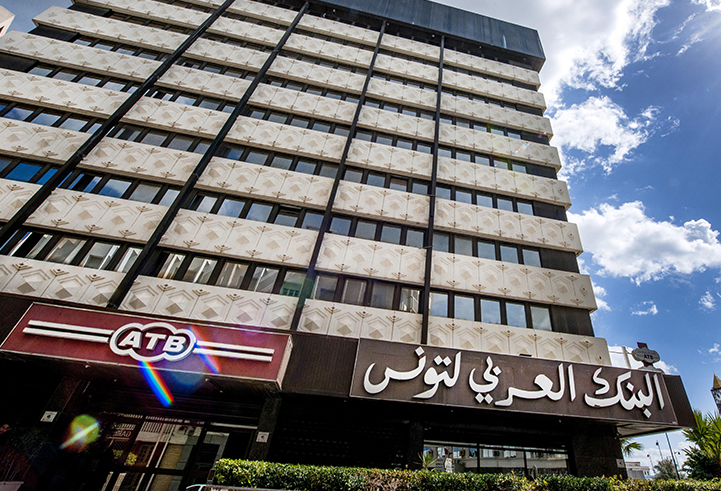
\includegraphics[width=0.75\textwidth]{atb_building.jpg}
\caption{ATB headquarters and organizational overview\cite{atb_logo}}
\label{fig:atb_logo}
\end{figure}
\FloatBarrier
%------------------------------------------------
\subsection{ATB Company Datasheet}

Table~\ref{tab:fiche_atb} presents the key factual information related to the host organization.

\begin{table}[H]
\centering
\renewcommand{\arraystretch}{1.6}
\caption{Arab Tunisian Bank (ATB) Company Datasheet}
\label{tab:fiche_atb}
\begin{tabular}{|p{5cm}|p{9cm}|}
\hline
\rowcolor{blue!15}
\textbf{Field} & \textbf{Details} \\ \hline
Full Name & Arab Tunisian Bank (ATB) \\ \hline
Date of Establishment & June 30, 1982 \\ \hline
Headquarters & 9 Rue H\'edi Nouira, 1001 Tunis, Tunisia \\ \hline
Phone & +216 71 351 155 \\ \hline
General Director & Riadh Hajjej \\ \hline
Share Capital & 128 million Tunisian Dinars \\ \hline
Commercial Register & B 167001997 \\ \hline
Branch Hours & Monday to Friday: 8:00--12:00 and 13:00--16:30 \\ \hline
Contact Email & qualite.retail@atb.com.tn \\ \hline
Website & \url{https://www.atb.com.tn} \\ \hline
LinkedIn & \url{https://www.linkedin.com/company/arabtunisianbank/} \\ \hline
\end{tabular}
\end{table}
\FloatBarrier

%================================================
\section{Project Presentation}

\subsection{Project Context}

This final year project, carried out as part of a four-month internship (April to July 2025)
at the ATB, validates the competencies acquired during the Bachelor's degree in Management
Information Systems, speciality Business Intelligence. It constitutes a key milestone towards
obtaining the diploma from ITBS.

Currently, the \textit{Direction March\'{e} Entreprises} of the ATB relies on a semi-automated
process for monitoring and controlling its commercial activities. Data is manually collected
from various sources and consolidated into Microsoft Excel spreadsheets to generate static
reporting dashboards. While this system offers a baseline level of reporting, it presents
significant limitations that hinder rapid and well-informed decision-making.

\subsection{Problem Statement}

The ATB's \textit{Direction March\'{e} Entreprises} currently relies on a manual data
consolidation process. Analysts collect records from multiple heterogeneous sources and
centralize them in Microsoft Excel files to produce static reporting dashboards.

Although this approach provides a baseline level of reporting, it exhibits significant
structural limitations:

\begin{itemize}
    \item Manual data entry is a frequent source of inaccuracies and inconsistencies.
    \item Static dashboards prevent interactive data exploration and drill-down analysis.
    \item The system cannot scale to handle growing data volumes efficiently.
    \item The reporting process is time-consuming and slows decision cycles.
    \item Limited decision reactivity reduces the speed and quality of strategic responses.
    \item The risk of analytical errors negatively impacts strategic choices.
\end{itemize}

The absence of a centralized and automated analytical infrastructure prevents optimal
exploitation of available data. It therefore becomes essential to design an intelligent,
automated system capable of consolidating, transforming, and visualizing data to support
rapid and evidence-based decision-making at the ATB.

\subsection{Project Objectives}

The primary objective of this project is to design a data management solution enabling rapid
and informed decision-making at the ATB. By aggregating and analyzing available data, this
solution aims to identify gaps between set objectives and achieved results, thereby facilitating
relevant strategic adjustments. The specific sub-objectives are:

\begin{enumerate}
    \item \textbf{Automated Data Ingestion Pipeline:} Design and deploy an automated ETL
    pipeline using \textbf{Airbyte} to extract data from heterogeneous operational sources
    and load it into a centralized staging area.

    \item \textbf{Data Warehouse and Dimensional Modeling:} Build a structured analytical
    data warehouse using a dimensional approach (star/constellation schema) hosted on
    \textbf{SQL Server} to enable multidimensional analysis and historical tracking.

    \item \textbf{Data Transformation Layer:} Implement a transformation layer using
    \textbf{dbt (data build tool)} to clean, model, and prepare data for analytical
    consumption, with full lineage tracking and documentation.

    \item \textbf{Pipeline Orchestration:} Deploy \textbf{Apache Airflow} to automate,
    schedule, and monitor the end-to-end data pipeline, ensuring reliability,
    observability, and fault alerting.

    \item \textbf{Customer Risk Scoring with Machine Learning:} Develop and integrate an
    \textbf{XGBoost}-based customer risk scoring model to classify clients by risk profile,
    enriching the analytical layer with predictive intelligence.

    \item \textbf{Interactive BI Dashboards:} Deliver a multi-page \textbf{Streamlit}
    dashboard enabling ATB managers and analysts to visualize KPIs, monitor commercial
    activity, and make data-driven decisions in real time.
\end{enumerate}

%================================================
\section{Study of the Existing System}

In order to design a relevant solution, an analysis of the tools currently used at ATB and
in the broader banking BI domain was conducted. Two tools are examined: Microsoft Excel,
the internal reporting tool used by the \textit{Direction March\'{e} Entreprises}, and
Microsoft Power BI, one of the most widely adopted external BI platforms. Since both tools
are part of ATB's analytical landscape, they are analyzed jointly below.

%------------------------------------------------
\subsection{Combined Analysis: Microsoft Excel and Microsoft Power BI}

\textbf{General Presentation}

The ATB's \textit{Direction March\'{e} Entreprises} currently uses \textbf{Microsoft Excel}
as its primary tool for data consolidation and reporting. Analysts manually collect data from
various operational systems and enter it into spreadsheets to produce reporting tables.
Alongside this internal practice, \textbf{Microsoft Power BI} --- one of the most widely
adopted Business Intelligence platforms in the industry --- serves as the external benchmark
for comparison. Power BI enables organizations to connect to multiple data sources, build
interactive dashboards, and share analytical reports across the organization via the cloud.

\begin{figure}[H]
\centering

\begin{minipage}{0.45\textwidth}
    \centering
    
\includegraphics[height=1.5cm]{excel_logo.png}
    \captionof{figure}{Microsoft Excel (ATB Internal Tool)\cite{excel_logo}}
    \label{fig:excel_logo}
\end{minipage}
\hfill
\begin{minipage}{0.45\textwidth}
    \centering
    
\includegraphics[height=1.5cm]{powerbi_logo.png}
    \captionof{figure}{Microsoft Power BI (Industry Benchmark)\cite{powerbi_logo}}
    \label{fig:powerbi_logo}
\end{minipage}

\end{figure}

\textbf{Detailed Analysis}

Table~\ref{tab:combined_analyse} presents a structured side-by-side analysis of both tools
across key BI dimensions.

\begin{table}[H]
\centering
\small
\renewcommand{\arraystretch}{1.3}
\caption{Combined analysis of Microsoft Excel and Microsoft Power BI}
\label{tab:combined_analyse}
\begin{tabular}{|p{3.5cm}|p{5.2cm}|p{5.2cm}|}
\hline
\rowcolor{blue!15}
\textbf{Aspect} & \textbf{Microsoft Excel (ATB Internal)} & \textbf{Microsoft Power BI (Industry)} \\ \hline
Data Collection & Manual entry from various operational sources & Automated connectors to 100+ data sources \\ \hline
Storage & Local or shared Excel files; no governance & Cloud-based or on-premise; role-based access \\ \hline
Processing & Formulas and pivot tables & DAX language for KPIs and calculated measures \\ \hline
Visualization & Static charts and tables & Interactive dashboards with drag-and-drop \\ \hline
Data Refresh & None; fully manual updates & Scheduled automated refresh \\ \hline
ML Integration & Absent & Limited; requires additional Azure ML services \\ \hline
Licensing & Included in Microsoft Office & High per-user licensing cost \\ \hline
\end{tabular}
\end{table}

Table~\ref{tab:combined_synthese} presents the combined strengths and weaknesses of both tools.

\begin{table}[H]
\centering
\small
\renewcommand{\arraystretch}{1.3}
\caption{Summary of strengths and weaknesses: Excel and Power BI}
\label{tab:combined_synthese}
\begin{tabular}{|p{3.5cm}|p{5.2cm}|p{5.2cm}|}
\hline
\rowcolor{blue!15}
\textbf{Dimension} & \textbf{Strengths} & \textbf{Weaknesses} \\ \hline
Microsoft Excel &
  Widely mastered; flexible for ad-hoc calculations; no infrastructure required; easy report sharing via email &
  Manual and error-prone; no versioning, lineage, or governance; static dashboards; not scalable \\ \hline
Microsoft Power BI &
  Intuitive interface; native connectors to many sources; automated refresh; widely documented &
  High licensing cost; cloud dependency; limited ML integration; restricted programmatic customization \\ \hline
\end{tabular}
\end{table}
\FloatBarrier

%================================================
\section{Synthesis of the Existing System Study}

The study of ATB's current Excel-based approach and the analysis of Power BI reveal a
strategic gap: on one hand, a fully manual, error-prone process with no scalability; on the
other, a proprietary BI platform that, while powerful for visualization, lacks native support
for custom ML integration and open-source pipeline orchestration. The solution developed for
ATB adopts a modern, open-source, data-driven architecture to address all these limitations:

\begin{itemize}
    \item \textbf{Data Automation:} Eliminates manual data collection
    through automated, scheduled ingestion pipelines.

    \item \textbf{Data Engineering:} Provides a structured,
    versionable, and documented transformation layer feeding a governed analytical warehouse.

    \item \textbf{Predictive Intelligence:} Complements descriptive BI with
    customer risk scoring, enabling proactive decision-making.

    \item \textbf{Interactive Dashboards:} Delivers fully customizable,
    programmatically controlled dashboards aligned with ATB's specific analytical needs.
\end{itemize}

%================================================
\section{Proposed Solution}
\label{sec:solution_proposee}

In response to the limitations of ATB's manual reporting process and the strategic gap
identified in the existing solutions study, we propose the design and implementation of a
\textbf{full-stack Business Intelligence and Machine Learning Platform}. This solution is
structured as a unified decision-support platform, organized across several coherent
functional and architectural modules.

\begin{figure}[H]
\centering
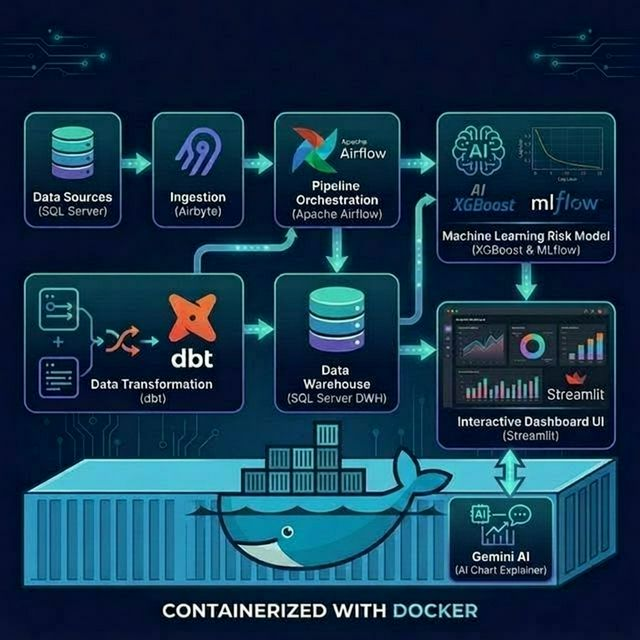
\includegraphics[width=0.92\textwidth]{figures/figure5.png}
\caption{Overview of the proposed Platform}
\label{fig:proposed_solution_overview}
\end{figure}
\FloatBarrier

\subsection{Functional Modules of the Solution}

The proposed solution is organized around a modular architecture ensuring automated
acquisition, structured storage, governed transformation, predictive enrichment, and
interactive restitution of data:

\begin{enumerate}
    \item \textbf{Automated Data Ingestion Module (Airbyte):}
    This component automates the extraction of data from heterogeneous operational sources
    and loads it into a centralized staging area. It resolves the data dispersion problem
    by consolidating raw information into a clean, normalized repository.

    \item \textbf{Data Warehouse and Dimensional Modeling (SQL Server):}
    To enable multidimensional analytical queries, the solution integrates a data warehouse
    modeled using a dimensional approach. This structure historizes facts related to client
    activities and risk while linking them to shared dimension tables representing clients,
    agencies, and time periods.

    \item \textbf{Data Transformation Layer (dbt):}
    The transformation layer uses \textbf{dbt (data build tool)} to apply business logic
    and quality rules to raw data. It produces clean, documented, and version-controlled
    analytical models with full data lineage.

    \item \textbf{Pipeline Orchestration (Apache Airflow):}
    The end-to-end data pipeline is orchestrated and monitored using \textbf{Apache Airflow}.
    DAGs (Directed Acyclic Graphs) schedule and coordinate ingestion, transformation, and
    ML scoring tasks, ensuring observability and controlled re-execution.

    \item \textbf{Predictive Scoring Engine (XGBoost):}
    At the core of the predictive layer, an \textbf{XGBoost}-based machine learning model
    scores customers by risk profile. Trained on historical behavioral and financial data,
    it classifies clients into risk categories, enriching the dashboards with proactive
    intelligence.

    \item \textbf{Decision Monitoring Interface (Streamlit Dashboard):}
    An interactive multi-page portal is made available to ATB managers and analysts. It
    provides dynamic visualization of KPIs, client risk distribution, agency performance,
    and temporal trends, enabling real-time data-driven decisions.
\end{enumerate}

\subsection{Functional Comparison with the Existing System}

Table~\ref{tab:comparatif_existant_solution} highlights the functional contribution of the
proposed solution compared to existing approaches.

\begin{table}[H]
\centering
\small
\renewcommand{\arraystretch}{1.5}
\caption{Functional Comparison: Existing Approaches vs.\ ATB BI Platform}
\label{tab:comparatif_existant_solution}
\begin{tabular}{|p{3.2cm}|p{3.3cm}|p{3.3cm}|p{4.3cm}|}
\hline
\rowcolor{blue!15}
\textbf{Criterion} & \textbf{Excel Reports} & \textbf{Power BI} & \textbf{ATB BI Platform} \\ \hline
Automation & Fully manual & Partial (scheduled refresh) & Daily automated pipeline (Airflow) \\ \hline
Data Model & None & Proprietary & Constellation schema (dbt + SQL Server) \\ \hline
Historical Tracking & Not supported & Limited & Time-versioned fact tables \\ \hline
Risk Analytics & Absent & Ad-hoc only & 3-pillar composite scoring model \\ \hline
ML Prediction & Absent & Custom visuals only & XGBoost + SHAP explainability \\ \hline
Interactivity & Static charts & Semi-interactive & Streamlit multi-page dashboard \\ \hline
Data Quality & Manual & No governance & Automated dbt tests \\ \hline
Reproducibility & Low & Low & Version-controlled pipeline \\ \hline
Licensing Cost & Included in Office & High per-user fee & Fully open-source \\ \hline
\end{tabular}
\end{table}

\subsection{Expected Benefits for ATB}

The deployment of this solution brings major strategic added value for the organization:

\begin{itemize}
    \item \textbf{Productivity and Automation:} Automated ingestion and transformation reduce
    data preparation time from hours to minutes, freeing analysts for higher-value tasks.

    \item \textbf{Standardization and Objectivity:} A governed, version-controlled data
    pipeline ensures consistent, auditable, and reproducible analytical outputs.

    \item \textbf{Proactive Predictive Intelligence:} The XGBoost risk model enables ATB to
    anticipate customer risk profiles rather than react to incidents.

    \item \textbf{Real-Time Decision Support:} Streamlit dashboards provide instant access
    to up-to-date KPIs, enabling management to monitor performance in real time.

    \item \textbf{Open-Source and Data Sovereignty:} The fully open-source stack eliminates
    vendor lock-in and licensing costs while keeping all data within ATB's infrastructure.
\end{itemize}

%================================================
\section{Project Methodological Framework}

\subsection{Comparison: Traditional vs.\ Agile Project Management}

Traditional project management relies on a sequential linear model (the waterfall cycle),
requiring exhaustive upfront planning structured into distinct successive phases. To clarify
the choice of methodology, Table~\ref{tab:comparaison_traditionnelle_agile} summarizes the
major differences between these two paradigms.

\begin{table}[H]
\small
\centering
\caption{Comparison of traditional and agile project management approaches}
\label{tab:comparaison_traditionnelle_agile}
\renewcommand{\arraystretch}{1.4}
\begin{tabular}{|p{2.8cm}|p{5.5cm}|p{5.5cm}|}
\hline
\rowcolor{blue!15}
\textbf{Characteristic} & \textbf{Traditional Approach} & \textbf{Agile Approach} \\
\hline
Project Structure & Sequential phases; each validated before advancing. & Iterative and incremental, favoring continuous adjustments. \\
\hline
Planning & Detailed upfront plan, difficult to change. & Adaptive planning evolving with the project. \\
\hline
Change Management & Changes are difficult and costly to integrate. & Changes are accepted and integrated fluidly. \\
\hline
Flexibility & Low; modifications are expensive mid-project. & High; rapid reactivity to evolving needs. \\
\hline
Communication & Formal, planned, and documented. & Continuous and collaborative within the team. \\
\hline
Deliverables & Fixed final deliverables, few intermediate revisions. & Frequent deliverable revisions at each iteration. \\
\hline
Testing & Tests performed at end of cycle. & Tests integrated at each iteration. \\
\hline
\end{tabular}
\end{table}

The comparative analysis highlights the significant advantages of the agile approach,
particularly in terms of flexibility, continuous collaboration, and adaptability.

%----------------------------------------------
\subsection{Comparison of Agile Methods: Scrum, Kanban, and XP}

Table~\ref{tab:comparaison_methodes_agiles} presents a comparison between the leading agile
frameworks.

\begin{table}[H]
\centering
\small
\caption{Comparison of agile methodologies}
\label{tab:comparaison_methodes_agiles}
\begin{tabular}{|p{2.8cm}|p{3.8cm}|p{3.8cm}|p{3.8cm}|}
\hline
\rowcolor{blue!15}
\textbf{Criteria} & \textbf{Scrum} & \textbf{XP} & \textbf{Kanban} \\
\hline
Planning & Start of each sprint with defined objectives & Planning games with team and client & Continuous Kanban-driven flow \\
\hline
Scope Changes & Integrated into next sprint & Continuous adaptation & Real-time priority adjustments \\
\hline
Key Roles & Scrum Master, Product Owner, Dev Team & Team and client & Team \\
\hline
Main Advantages & Productivity, scalability, team involvement & Code quality, reactivity & Quick setup, clear visualization \\
\hline
\end{tabular}
\end{table}

%----------------------------------------------
\subsection{Chosen Framework: Scrum}

In the context of this project, the \textbf{Scrum} framework was adopted as the overall
project management methodology. This agile approach, based on iterative and incremental
development, is well-suited to the evolving nature of requirements and the complexity of a
full-stack BI project.

Unlike rigid traditional methods, Scrum provides better visibility over progress, facilitates
mid-course adjustments, and encourages fluid communication through daily synchronization
points. The key advantages justifying this choice are:

\begin{itemize}
    \item Iterative, incremental, and adaptable approach.
    \item High responsiveness to changing requirements.
    \item Regular delivery of functional increments.
    \item Continuous improvement through retrospectives.
    \item Daily active team collaboration.
    \item Transparency in project tracking (backlogs, burndown charts)
    \item Reduced risk related to unforeseen changes.
    \item Better stakeholder satisfaction through frequent involvement.
\end{itemize}

%----------------------------------------------
\subsection{Scrum Roles}

The Scrum framework relies on three fundamental roles:

\begin{itemize}
    \item \textbf{Product Owner:} Representative of ATB stakeholders. Carries the product
    vision, defines and prioritizes functional requirements in the Product Backlog.

    \item \textbf{Scrum Master:} Guarantor of proper Scrum adherence. Removes impediments,
    facilitates collaboration, and protects the team from external disruptions.

    \item \textbf{Development Team:} Multidisciplinary team (data engineering, ML, BI) that
    is self-organized and responsible for delivering increments at each sprint.
\end{itemize}

%----------------------------------------------
\subsection{Scrum Artifacts}

\begin{itemize}
    \item \textbf{Product Backlog:} A prioritized and evolving list of requirements for the
    BI platform. Managed by the Product Owner.

    \item \textbf{Sprint Backlog:} A subset of the Product Backlog selected for a sprint,
    containing the objectives and tasks to complete.

    \item \textbf{Increment:} At the end of each sprint, a functional and deliverable result
    (e.g., an operational Airbyte pipeline, a validated dbt model, a deployed Streamlit
    dashboard).
\end{itemize}

%----------------------------------------------
\subsection{Scrum Events}

The sprint is structured by five key events:

\begin{itemize}
    \item \textbf{Sprint:} Fixed-duration iteration (2--4 weeks) producing a functional
    product version.

    \item \textbf{Sprint Planning:} Meeting defining the sprint objectives and selected items.

    \item \textbf{Daily Scrum:} 15-minute daily meeting sharing progress, plans, and blockers.

    \item \textbf{Sprint Review:} Demonstration of the completed increment to stakeholders.

    \item \textbf{Sprint Retrospective:} Analysis meeting to improve team practices.
\end{itemize}

These events create a collaborative, transparent, and value-delivery oriented framework.

%----------------------------------------------
\subsection{Comparison of Data Science Methodologies}

Well-structured data science methodologies are essential for the reproducibility and quality
management of analytical pipelines. Three major methodologies are compared in
Table~\ref{tab:comparaison_data_sciences}.

\begin{table}[H]
\small
\centering
\caption{Comparison of Data Mining and Machine Learning Methodologies}
\label{tab:comparaison_data_sciences}
\renewcommand{\arraystretch}{1.4}
\begin{tabular}{|p{2.5cm}|p{3.5cm}|p{3.5cm}|p{4cm}|}
\hline
\rowcolor{blue!15}
\textbf{Criteria} & \textbf{CRISP-DM} & \textbf{CRISP-ML(Q)} & \textbf{KDD} \\
\hline
Target & Generalist data mining & Machine Learning models & Large-scale databases \\
\hline
Advantage & Industry standard, well documented & ML-specific, integrates MLOps and QA & Proven for raw database exploration \\
\hline
Disadvantage & Ignores model drift in production & Requires mature MLOps infrastructure & Complex, technically demanding \\
\hline
\end{tabular}
\end{table}

%----------------------------------------------
\subsection{Chosen Tripartite Methodological Architecture}

At the conclusion of the comparative analysis, it became clear that no single method covers
all of the complex components of this project. A \textbf{tripartite methodological
architecture} was therefore adopted, where three methodologies are logically interlocked:

\begin{itemize}
    \item \textbf{Scrum (The Global Framework):} Used as the overall Project Management
    methodology, organizing the development calendar into 3 iterative Sprints structured as
    distinct functional and deliverable Releases.

    \item \textbf{CRISP-ML (The Technical Framework):} Used within Sprints dedicated to
    data engineering and machine learning, guiding ETL design, dimensional data warehouse
    modeling, XGBoost model training, MLOps tracking, and continuous monitoring.

    \item \textbf{GIMSI (The BI Business Framework):} Used within Sprints dedicated to
    dashboard development guiding KPI selection and visual design of decision-support
    interfaces for ATB management.
\end{itemize}

Table~\ref{tab:methodologie_tripartite} presents the tripartite methodological architecture.

\begin{table}[H]
\small
\centering
\caption{Tripartite methodological architecture of the ATB BI project}
\label{tab:methodologie_tripartite}
\begin{tabular}{|p{3cm}|p{4.5cm}|p{6.5cm}|}
\hline
\rowcolor{blue!15}
\textbf{Level} & \textbf{Methodology} & \textbf{Application in the Project} \\
\hline
Macro (Management) & Scrum & Global planning (3 Sprints/Releases), backlog tracking, incremental deliveries \\
\hline
Micro (Technical) & CRISP-ML & Airbyte ingestion, dbt transformation, DWH modeling, XGBoost training, MLflow tracking \\
\hline
Micro (Business) & GIMSI & Design and development of Streamlit dashboards for ATB management \\
\hline
\end{tabular}
\end{table}

The three following subsections detail each methodology and its concrete application.

%----------------------------------------------
\subsection{Data Science Methodology: CRISP-ML}

CRISP-ML (Cross-Industry Standard Process for Machine Learning) is a specialized, industry-standard
methodology designed to structure the end-to-end machine learning lifecycle. Unlike traditional data mining processes,
CRISP-ML explicitly incorporates MLOps requirements, quality assurance gates, experiment tracking, and continuous monitoring into six cyclical and iterative phases.

Figure~\ref{fig:crispml} illustrates the cyclic nature of the CRISP-ML methodology.

\begin{figure}[H]
\centering
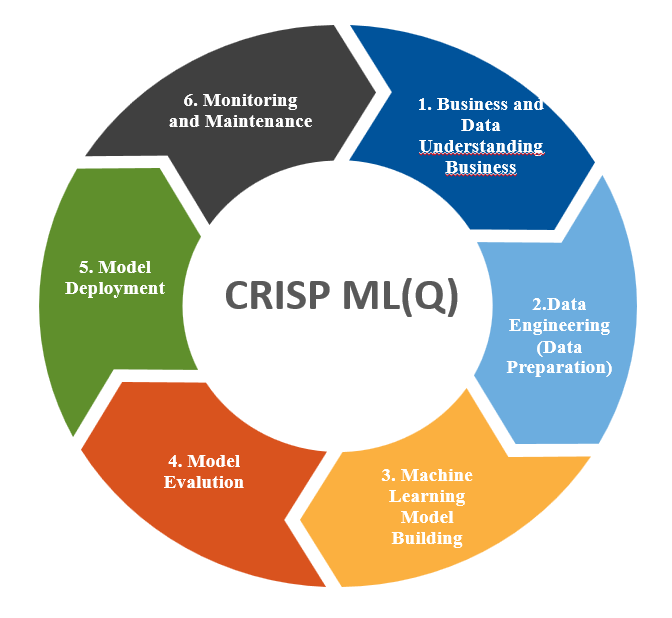
\includegraphics[width=0.42\textwidth]{crispml.png}
\caption{Cyclic representation of the CRISP-ML methodology\cite{crispml}}
\label{fig:crispml}
\end{figure}
\FloatBarrier

Table~\ref{tab:crispml_phases} presents the six phases of CRISP-ML and their concrete
application in the ATB BI project.

\begin{table}[H]
\small
\centering
\renewcommand{\arraystretch}{1.5}
\caption{The 6 phases of CRISP-ML applied to the ATB BI project}
\label{tab:crispml_phases}
\begin{tabular}{|c|p{4cm}|p{7.5cm}|}
\hline
\rowcolor{blue!25}
\textbf{Phase} & \textbf{CRISP-ML Phase Name} & \textbf{Application in the ATB Project} \\
\hline
1 & Business \& Data Understanding & Defining \textit{Direction March\'{e} Entreprises} operational goals, risk scoring requirements, and evaluating data source availability \\
\hline
2 & Data Engineering \& Preparation & Ingestion via Airbyte, cleansing and transformation via dbt into DWH, leakage-free feature engineering (34 indicators) \\
\hline
3 & ML Model Engineering & XGBoost customer risk scoring model training, hyperparameter optimization, MLflow experiment tracking \\
\hline
4 & Quality Assurance \& Evaluation & Performance validation against quality gates (F1 $\geq 0.70$, ROC-AUC $\geq 0.80$), confusion matrix, SHAP explainability \\
\hline
5 & Model Deployment & Promotion in MLflow Model Registry, integration into Streamlit dashboard (\textit{ML Risk Intelligence}), interactive risk predictor \\
\hline
6 & Model Monitoring \& Maintenance & Airflow orchestration (\texttt{dag\_ml\_pipeline}), automated batch scoring into DWH, disagreement alerting \\
\hline
\end{tabular}
\end{table}
\FloatBarrier

%----------------------------------------------
\subsection{Application of Scrum to Project Development}

The iterative nature of the ATB BI project, characterized by evolving data requirements and
incremental deliverable validation by ATB stakeholders, makes the classical cascade approach
unsuitable. The Scrum framework organizes work into fixed-duration Sprints (three to four
weeks), structured into functional and deliverable Releases.

Figure~\ref{fig:scrum} illustrates the Scrum development cycle applied to this project.

\begin{figure}[H]
\centering
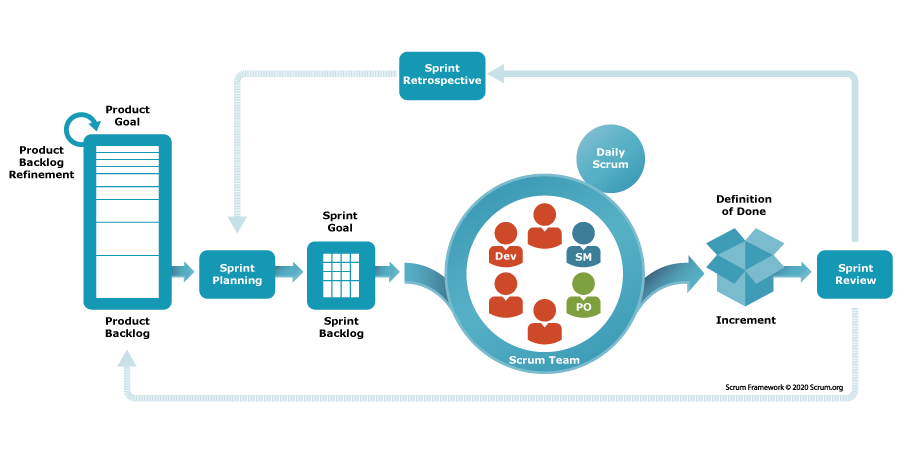
\includegraphics[width=0.42\textwidth]{figures/scrum.png}
\caption{Cyclic representation of Scrum methodology\cite{scrum}}
\label{fig:scrum}
\end{figure}
\FloatBarrier

%----------------------------------------------
\subsection{Application of GIMSI to Business Intelligence}

GIMSI (G\'{e}n\'{e}rer des Indicateurs de performance pour le Management Strat\'{e}gique de
l'Information) guarantees that each KPI selected for the ATB dashboards is aligned with the
strategic objectives of the organization. It ensures the BI solution is a genuine
decision-support instrument, not merely a technical deliverable.

Table~\ref{tab:gimsi_application} presents the application of GIMSI to the ATB Streamlit
dashboard.

\begin{table}[H]
\small
\centering
\caption{Application of the GIMSI methodology to the ATB Streamlit Dashboard}
\label{tab:gimsi_application}
\begin{tabular}{|p{3.5cm}|p{10cm}|}
\hline
\rowcolor{blue!15}
\textbf{GIMSI Phase} & \textbf{Application in the ATB Project} \\
\hline
Needs Analysis & Identification of KPIs for the \textit{Direction March\'{e} Entreprises}: agency performance, client risk, objective tracking \\
\hline
Design & Wireframing of dashboard pages: global overview, risk analysis, agency performance, client segmentation \\
\hline
Development & Streamlit implementation with Plotly visualizations and SQL Server connection \\
\hline
Deployment & Production release of the interactive multi-page dashboard for ATB managers \\
\hline
\end{tabular}
\end{table}
\FloatBarrier

\bigskip

Figure~\ref{fig:gimsi-dashboard} illustrates the general architecture of a GIMSI-based
decision-making information system, as applied to the ATB dashboard design.

\begin{figure}[H]
\centering
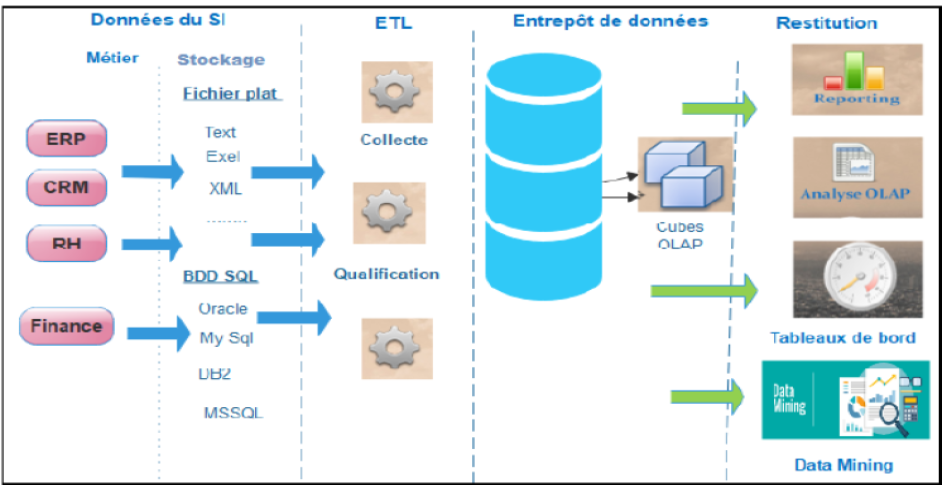
\includegraphics[width=0.8\textwidth]{gimsi.png}
\caption{Architecture of a GIMSI-based decision-support system\cite{gimsi}}
\label{fig:gimsi-dashboard}
\end{figure}
\FloatBarrier

%----------------------------------------------
% GANTT DIAGRAM
%----------------------------------------------

Figure~\ref{fig:gantt_atb} presents the Gantt chart synchronizing the three Releases, the
three Sprints, and the three methodologies of the ATB BI project across 12 weeks.

\begin{figure}[H]
\centering
\begin{tikzpicture}[
    xscale=0.85,
    yscale=1.2,
    every node/.style={font=\scriptsize},
    barre/.style={rectangle, rounded corners=3pt, minimum height=0.65cm, text centered,
                  text=white, font=\bfseries\scriptsize},
    trait/.style={thick, gray!50, dashed, -stealth}
]

% WEEK AXIS (12 weeks)
\draw[->, thick, draw=black!70] (0,0) -- (12.8,0)
    node[right, font=\bfseries\footnotesize] {Weeks};
\foreach \x in {0,2,4,6,8,10,12} {
    \draw[thick, draw=black!70] (\x, 0.1) -- (\x,-0.2);
    \node[below, font=\bfseries\small, text=black!80] at (\x,-0.3) {\x};
}
\foreach \x in {2,4,6,8,10,12} {
    \draw[very thin, gray!20] (\x,0) -- (\x,8.0);
}

% RELEASES
\node[anchor=east, font=\bfseries\footnotesize, text=black!70] at (-0.5,7.5) {RELEASES};
\node[barre, fill=green!55!black, minimum width=4.0cm]
    at (2,  7.5) {Release 1 --- Pipeline \& DWH};
\node[barre, fill=teal!70!black,  minimum width=4.0cm]
    at (6,  7.5) {Release 2 --- ML \& Scoring};
\node[barre, fill=purple!65,      minimum width=4.0cm]
    at (10, 7.5) {Release 3 --- Dashboard BI};

% SCRUM
\node[anchor=east, font=\bfseries\footnotesize, text=orange!90!black] at (-0.5,5.5) {SCRUM};
\node[barre, fill=orange!85, minimum width=3.8cm] at (2,  5.5) {Sprint 1};
\node[barre, fill=orange!70, minimum width=3.8cm] at (6,  5.5) {Sprint 2};
\node[barre, fill=orange!85, minimum width=3.8cm] at (10, 5.5) {Sprint 3};

% CRISP-ML
\node[anchor=east, font=\bfseries\footnotesize, text=blue!80!black] at (-0.5,3.0) {CRISP-ML};
\node[barre, fill=blue!80, minimum width=1.6cm] at (0.9, 3.0) {P1: Business};
\node[barre, fill=blue!70, minimum width=3.2cm] at (3.5, 3.0) {P2-3: Data};
\node[barre, fill=blue!80, minimum width=3.2cm] at (7,   3.0) {P4: Modeling};
\node[barre, fill=blue!70, minimum width=1.6cm] at (10,  3.0) {P5: Eval.};
\node[barre, fill=blue!80, minimum width=1.6cm] at (11.5,3.0) {P6: Deploy};

% GIMSI
\node[anchor=east, font=\bfseries\footnotesize, text=teal!90!black] at (-0.5,1.0) {GIMSI};
\node[barre, fill=teal!80, minimum width=2.5cm] at (9,    1.0) {1. KPI Analysis};
\node[barre, fill=teal!70, minimum width=1.8cm] at (11,   1.0) {2. Wireframe};
\node[barre, fill=teal!80, minimum width=1.5cm] at (12.2, 1.0) {3. UI};

% ARROWS
\draw[trait] (2,  7.1) -- (2,  5.9);
\draw[trait] (6,  7.1) -- (6,  5.9);
\draw[trait] (10, 7.1) -- (10, 5.9);
\draw[trait] (10, 5.1) -- (10, 1.4);
\draw[trait] (6,  5.1) -- (6,  3.4);

% TITLE
\node[font=\bfseries\large, text=black!80] at (6.2, 9.0)
    {12 Weeks --- 3 Releases --- 3 Sprints --- Tri-Methodological Planning};

\end{tikzpicture}
\caption{Gantt chart: 3 Releases, 3 Sprints, and 3 methodologies of the ATB BI project
         over 12 weeks.}
\label{fig:gantt_atb}
\end{figure}

%================================================
\section{Conclusion}

This chapter has established the general framework of the project. The presentation of the
Arab Tunisian Bank (ATB)  its history, market segments, organizational structure,
missions, and branch network provides the institutional context within which this
internship was conducted.

The analysis of ATB's current data management process within the \textit{Direction March\'{e}
Entreprises} has highlighted its significant limitations: a manual, error-prone, and
non-scalable Excel-based reporting workflow that hinders rapid and informed strategic
decision-making.

The comparative study of existing approaches (the internal Excel-based process and the
Power BI platform) confirmed the absence of a solution that simultaneously integrates
automated data collection, governed transformation, predictive intelligence, and fully
customizable interactive dashboards within an open-source, cost-free architecture.

Finally, a rigorous tripartite methodological architecture has been defined and
justified: Scrum as the global project management framework, CRISP-ML to
guide data engineering and machine learning pipeline development, and GIMSI to
orient the design of decision-support dashboards for ATB management.

The following chapter presents the state of the art of the technical domains mobilized for
the design of this Business Intelligence and Machine Learning platform.

%================================================
% CHAPTER 2: STATE OF THE ART AND REQUIREMENTS SPECIFICATION
% ATB BI PROJECT — English version aligned with NotMychapter2 structure
%================================================
\chapter{State of the Art and Requirements Specification}

\section{Introduction}

This chapter establishes the theoretical and functional foundations of the ATB Business
Intelligence and Machine Learning project. It is structured around three objectives:
(1) to position the project within the existing scientific literature on Business Intelligence,
machine learning, data warehousing, and MLOps; (2) to justify every architectural and
algorithmic choice through a systematic review of the relevant technical domains; and
(3) to provide the operational conceptual framework used to design the ATB BI platform,
from raw CSV ingestion to supervised risk classification and interactive dashboarding.

The approach follows the structure recommended by our academic supervisor: general concepts
and state of the art are presented first, followed by their specific application to the
banking sector and to this project, ensuring that the chapter is understandable to a reader
unfamiliar with the field.


%================================================
\section{State of the Art: Fundamentals}
%================================================

%----------------------------------------------
\subsection{Business Intelligence: Definitions and Domains}
%----------------------------------------------

Business Intelligence (BI) refers to the set of methodologies, architectures, tools, and
processes used to transform raw operational data into reliable, structured information
supporting managerial decision-making \cite{chaudhuri2011}. According to Chaudhuri et al.\
\cite{chaudhuri2011}, BI systems typically combine data integration, multidimensional
storage, analytical querying, and visual reporting into a unified decision-support chain.

Eckerson \cite{eckerson2010} defines BI more broadly as a discipline that enables
organisations to convert data into insights and insights into actions. He distinguishes
three levels of analytical maturity:

\begin{itemize}
    \item \textbf{Descriptive analysis}: understanding what has happened through historical
    reporting, dashboards, and KPI monitoring.
    \item \textbf{Diagnostic analysis}: understanding why it happened through drill-down,
    segmentation, and correlation exploration.
    \item \textbf{Predictive analysis}: anticipating what will happen through statistical
    models and machine learning integrated into the BI layer.
\end{itemize}

\textbf{Main domains of Business Intelligence}

Table~\ref{tab:bi_domains_general} summarises the principal analytical domains that
constitute a complete BI system.

\begin{table}[H]
\centering
\small
\caption{Principal domains of a Business Intelligence system}
\label{tab:bi_domains_general}
\begin{tabular}{|p{3.2cm}|p{9cm}|}
\hline
\rowcolor{blue!15}
\textbf{Domain} & \textbf{Role} \\
\hline
Data Integration & Extracts data from heterogeneous operational sources and loads it into
a centralised staging area. \\
\hline
Data Warehousing & Organises data into dimensional models (star, snowflake, or constellation
schemas) optimised for analytical queries \cite{kimball2013}. \\
\hline
Data Transformation & Applies business logic, quality rules, and enrichment to prepare
data for analytical consumption. \\
\hline
Machine Learning & Extends descriptive BI with predictive and prescriptive capabilities
through supervised and unsupervised models. \\
\hline
Data Visualisation & Delivers interactive dashboards, KPI boards, and reports to
business decision-makers. \\
\hline
MLOps & Governs the lifecycle of production ML models through experiment tracking,
versioning, deployment, and drift monitoring. \\
\hline
\end{tabular}
\end{table}

\begin{figure}[H]
\centering
\begin{tikzpicture}[
    box/.style={rectangle, draw=blue!80, thick, fill=blue!10, text width=3.0cm,
    align=center, minimum height=0.9cm, rounded corners=4pt, font=\small\bfseries},
    arrow/.style={->, thick, blue!60, >=stealth}
]
\node[box, fill=blue!15] (bi) at (0,0) {Business Intelligence};
\node[box, fill=blue!20] (integration) at (0,-1.6) {Data Integration};
\node[box, fill=cyan!20] (dwh) at (-5.0,-3.2) {Data Warehouse};
\node[box, fill=orange!20] (ml) at (0,-3.2) {Machine Learning};
\node[box, fill=green!20] (viz) at (5.0,-3.2) {Data Visualization};
\node[box, fill=red!15] (mlops) at (0,-4.8) {MLOps};

\draw[arrow] (bi) -- (integration);
\draw[arrow] (integration) -- (dwh);
\draw[arrow] (integration) -- (ml);
\draw[arrow] (integration) -- (viz);
\draw[arrow] (ml) -- (mlops);
\end{tikzpicture}
\caption{Hierarchy of analytical domains in a Business Intelligence system\cite{chaudhuri2011}}
\label{fig:bi_domain_hierarchy}
\end{figure}
\FloatBarrier
\FloatBarrier

%----------------------------------------------
\subsection{Business Intelligence for Banking}
%----------------------------------------------

Banks rely on BI systems to monitor customer behaviour, detect risk exposure, analyse
commercial performance, and support regulatory compliance \cite{bcbs2011}. Unlike generic
dashboards, banking BI must handle sensitive customer information, account-level financial
metrics, compliance indicators, and traceable risk calculations that can be audited by
internal control teams.

According to the Basel Committee on Banking Supervision \cite{bcbs2011}, effective banking
supervision requires institutions to maintain consolidated, accurate, and timely data on
their customer base, credit exposures, and compliance posture. BI platforms directly address
this requirement by providing governed, auditable analytical pipelines.

In the ATB project, the banking context is represented by two major analytical domains:

\begin{itemize}
    \item \textbf{Customer portfolio analytics}: customer distribution by gender, employment
    status, nationality, sector, industry, target segment, branch, account count, balances,
    and overdraft activity.
    \item \textbf{Customer risk and compliance analytics}: KYC completeness, PEP status,
    compliance flags, posting restrictions, account behaviour, salary availability, dependent
    load, and composite risk scoring \cite{fatf2012}.
\end{itemize}

The ATB project therefore transforms raw operational banking records into a decision-support
platform covering three levels of analysis: descriptive (portfolio dashboards), risk and
compliance (KYC, PEP, scoring), and predictive (ML risk classification).

%----------------------------------------------
\subsection{Machine Learning: Definitions and Learning Paradigms}
%----------------------------------------------

\subsubsection{Definition and Learning Paradigms}

Machine Learning (ML), defined by Mitchell \cite{mitchell1997}, enables computers to learn
from data without being explicitly programmed for each task. Rather than following hard-coded
rules, a machine learning system \textit{generalises} patterns observed in training data and
applies them to new, unseen examples. Mitchell's formal definition states:
\textit{``A computer program is said to learn from experience E with respect to some class of
tasks T and performance measure P, if its performance at tasks in T, as measured by P,
improves with experience E.''} \cite{mitchell1997}

The scientific literature distinguishes three main learning paradigms
\cite{hastie2009, bishop2006}. Table~\ref{tab:ml_paradigms_general} presents these three
paradigms.

\begin{table}[H]
\centering
\small
\caption{The three paradigms of machine learning}
\label{tab:ml_paradigms_general}
\begin{tabular}{|p{3.5cm}|p{4.5cm}|p{4.5cm}|}
\hline
\rowcolor{blue!15}
\textbf{Paradigm} & \textbf{Principle} & \textbf{Typical application} \\
\hline
\textbf{Supervised learning} & Learns from labelled examples
(input $\to$ known output) & Classification, regression, risk scoring \\
\hline
\textbf{Unsupervised learning} & Discovers hidden structures in
unlabelled data & Clustering, dimensionality reduction, anomaly detection \\
\hline
\textbf{Reinforcement learning} & Learns by trial-and-error interaction
with an environment & Robotics, game-playing, sequential optimisation \\
\hline
\end{tabular}
\end{table}

\subsubsection{Supervised Learning}

In supervised learning, the algorithm is trained on a dataset containing both input
variables and the expected outputs (labels). The objective is to learn a function
$f: X \to y$ that maps each input to its corresponding output, so that the model can
accurately predict the label of previously unseen data \cite{mitchell1997}. Bishop
\cite{bishop2006} distinguishes two types of supervised problems: \textbf{classification},
which predicts a discrete label (e.g., fraud / non-fraud, high risk / low risk), and
\textbf{regression}, which predicts a continuous numerical value (e.g., credit amount, churn
probability). The quality of a supervised model is measured by comparing its predictions
against a held-out test set, using metrics such as accuracy, precision, recall, F1-score,
and ROC-AUC.

Among the most effective supervised algorithms for structured tabular data are
\textbf{ensemble methods}: Random Forest \cite{breiman2001}, which combines multiple
decision trees through bagging, and \textbf{XGBoost} \cite{chen2016}, which uses gradient
boosting to sequentially correct the errors of previous trees. These two families have
dominated classification benchmarks in the scientific literature for over a decade
\cite{lessmann2015, baesens2003}.

\subsubsection{Unsupervised Learning}

Unsupervised learning processes unlabelled data to discover latent structures, groupings,
or relationships that are not explicitly encoded in the dataset. The goal is not to predict
a target variable but to understand the underlying organisation of the data
\cite{hastie2009}. Common techniques include:

\begin{itemize}
    \item \textbf{Clustering} (e.g., k-means, DBSCAN): groups observations into clusters
    of similar individuals based on their features.
    \item \textbf{Dimensionality reduction} (e.g., PCA, t-SNE): projects high-dimensional
    data into a lower-dimensional representation while preserving essential structure.
    \item \textbf{Anomaly detection}: identifies data points that deviate significantly from
    the learned normal distribution, used in fraud detection and operational monitoring.
\end{itemize}

Hastie et al.\ \cite{hastie2009} emphasise the utility of unsupervised methods for
exploratory data analysis, hypothesis generation, and pre-processing before supervised
model training. Although labels are absent, these techniques provide valuable insights
into data distributions and feature relationships.

\subsubsection{Reinforcement Learning}

Reinforcement learning (RL) involves an agent that interacts with a dynamic environment.
At each step, the agent takes an action, receives a reward or penalty, and updates its
policy to maximise cumulative reward over time \cite{hastie2009}. Unlike supervised
learning, RL does not require a labelled dataset; it learns from the consequences of its
own decisions. Well-known applications include game-playing agents (AlphaGo), robotics, and
dynamic pricing optimisation. However, RL requires a simulation environment and is
particularly suited to sequential decision-making problems where historical tabular data
alone is insufficient.

\begin{figure}[H]
\centering
\begin{tikzpicture}[
    node distance=0.8cm,
    box/.style={rectangle, draw=blue!70, thick, fill=blue!10, text width=4cm,
    text centered, minimum height=0.7cm, rounded corners=2pt, font=\small}
]
\node[box] (ml) {Machine Learning (ML)};
\node[box, below left=1cm and 1cm of ml, fill=green!10] (supervise) {Supervised Learning};
\node[box, below=1cm of ml, fill=orange!10] (non_supervise) {Unsupervised Learning};
\node[box, below right=1cm and 1cm of ml, fill=red!10] (renforcement) {Reinforcement Learning};
\draw[->, thick, blue!50] (ml) -- (supervise);
\draw[->, thick, blue!50] (ml) -- (non_supervise);
\draw[->, thick, blue!50] (ml) -- (renforcement);
\end{tikzpicture}
\caption{The three machine learning paradigms \cite{mitchell1997, hastie2009}}
\label{fig:ml_paradigms_fig}
\end{figure}

%----------------------------------------------
\subsection{Machine Learning for Banking}
%----------------------------------------------

The banking sector is one of the most data-rich domains and among the earliest adopters of
machine learning. Banks accumulate vast amounts of structured data: customer demographics,
account transaction histories, credit balances, behavioural indicators, and regulatory
attributes. This data richness makes banking a particularly fertile ground for supervised ML
applications \cite{hand1997}.

\subsubsection{(1)Principal Applications of ML in Banking}

Table~\ref{tab:ml_banking_applications} summarises the main application domains of machine
learning in the banking sector.

\begin{table}[H]
\centering
\small
\caption{Principal machine learning applications in banking}
\label{tab:ml_banking_applications}
\begin{tabular}{|p{4cm}|p{8cm}|}
\hline
\rowcolor{blue!15}
\textbf{Application domain} & \textbf{Description} \\
\hline
Credit scoring & Predicts the probability of default for loan applicants using financial
and behavioural features \cite{hand1997, lessmann2015}. \\
\hline
Fraud detection & Identifies anomalous transactions in real time using classification and
anomaly detection models \cite{breiman2001}. \\
\hline
Customer risk profiling & Segments customers by risk level based on compliance, financial
fragility, and behavioural signals \cite{baesens2003}. \\
\hline
Churn prediction & Anticipates customers likely to close accounts or reduce activity,
enabling proactive retention \cite{hastie2009}. \\
\hline
AML / KYC compliance & Flags suspicious transactions and incomplete customer due diligence
as required by FATF recommendations \cite{fatf2012}. \\
\hline
Portfolio analytics & Segments the customer portfolio by risk, sector, and behaviour to
support strategic decision-making \cite{bcbs2011}. \\
\hline
\end{tabular}
\end{table}

\subsubsection{(2)Supervised Models in Banking: Ensemble Methods}

Among the families of supervised algorithms, tree-based ensemble methods have established
themselves as the most reliable for structured banking data. Breiman's \textbf{Random
Forest} \cite{breiman2001} combines a large number of decision trees trained on bootstrap
samples of the data. By averaging their predictions, it reduces variance and achieves robust
generalisation even on noisy datasets. Its feature importance mechanism makes it inherently
interpretable at the variable level, which is essential in regulated environments.

\textbf{XGBoost} (eXtreme Gradient Boosting), introduced by Chen and Guestrin
\cite{chen2016}, builds trees iteratively where each new tree corrects the residual errors
of the previous ensemble. It introduces several regularisation mechanisms (L1 and L2
penalties on tree weights), handles sparse and missing data natively, and supports parallel
computation. Its superior performance on classification benchmarks across structured datasets
has made it the dominant algorithm in financial ML competitions and research publications
\cite{lessmann2015}.

\textbf{Model explainability: SHAP values}

In banking and regulatory contexts, a model must not only be accurate but also
\textit{explainable}. Lundberg and Lee \cite{lundberg2017} introduced SHAP (SHapley
Additive exPlanations), a game-theory-based framework that assigns to each feature a
contribution value for a specific prediction. SHAP values satisfy three desirable
properties: local accuracy (the sum of SHAP values equals the model's output),
missingness (features with value zero receive zero attribution), and consistency.
Their use in banking allows compliance teams to audit individual risk predictions and
verify that model outputs are driven by legitimate business features rather than
spurious correlations.

%----------------------------------------------
\subsection{Machine Learning and Banking Risk Prediction}
%----------------------------------------------

Banking risk prediction is a mature research field that combines statistical scoring,
financial analysis, customer behaviour modelling, and machine learning
\cite{hand1997, bravo2013}. The scientific literature provides strong empirical grounding
for the key design choices of automated risk scoring systems.

\subsubsection{(1)Foundational Works}

Hand and Henley \cite{hand1997} provide a landmark review of statistical classification
methods in consumer credit scoring, establishing that behavioural indicators---account
tenure, payment history, and activity patterns---are complementary to pure financial ratios
and significantly improve default prediction. Their work establishes the multi-signal
approach to risk assessment that has informed all subsequent credit scoring research.

Baesens et al.\ \cite{baesens2003}, in a large-scale benchmark across eight classification
algorithms on real banking datasets, demonstrate that ensemble methods (neural networks,
SVM, and ensemble trees) systematically outperform logistic regression on imbalanced risk
data. This study is a foundational reference justifying the use of tree-based classifiers
over simpler linear baselines in banking applications.

Lessmann et al.\ \cite{lessmann2015} extend this benchmark with more modern algorithms and
18 real-world credit datasets, confirming that gradient-boosted ensembles and random forests
consistently rank at the top for structured financial data. They also demonstrate that
accuracy alone is an insufficient evaluation metric under class imbalance and recommend
the F1-score, ROC-AUC, and PR-AUC as the primary evaluation criteria.

Dastile et al.\ \cite{dastile2020} conduct a systematic literature survey of credit scoring
models from 2000 to 2020, identifying three recurring challenges: (1)~class imbalance
between defaulters and non-defaulters; (2)~temporal instability of scoring models requiring
regular retraining; and (3)~the growing regulatory requirement for interpretable ML
predictions. They confirm that XGBoost and Random Forest dominate recent production
deployments.

Bravo et al.\ \cite{bravo2013} identify structural challenges specific to banking credit
scoring: data scarcity for rare risk events, selection bias in historical data, and the
need for reject inference when the approval process filters the training population. These
findings motivate the use of resampling techniques such as SMOTETomek to address class
imbalance, and held-out evaluation designs that prevent target leakage.

\subsubsection{(2)Regulatory Risk Drivers}

From a regulatory perspective, the FATF Recommendations \cite{fatf2012} establish that
incomplete Know Your Customer (KYC) data, Politically Exposed Person (PEP) exposure, and
compliance flags must be treated as \textit{primary} risk signals, preceding any financial
analysis. The Basel Committee on Banking Supervision \cite{bcbs2011} further formalises the
principle of multi-pillar risk assessment: compliance, financial, and behavioural dimensions
must be combined into a single, auditable, supervised risk view. This regulatory framework
directly justifies a weighted composite risk score combining three pillars:
\begin{equation}
\label{eq:global_risk_score}
\mathrm{GRS} = 0.40\,\mathrm{CRI} + 0.35\,\mathrm{FFS} + 0.25\,\mathrm{BRS},
\end{equation}
where $\mathrm{CRI}$, $\mathrm{FFS}$, and $\mathrm{BRS}$ denote respectively the
Compliance Risk Index, Financial Fragility Score, and Behavioural Risk Score, each
scaled to $[0,100]$.

\subsubsection{(3)Tree-Based Models for Risk Classification}

Based on the above literature, two tree-based ensemble models are retained and compared
for customer risk classification:

\begin{table}[H]
\centering
\small
\caption{Comparative justification of the ML models used for banking risk prediction}
\label{tab:atb_ml_models}
\begin{tabular}{|p{3cm}|p{5cm}|p{5.2cm}|}
\hline
\rowcolor{blue!15}
\textbf{Model} & \textbf{Properties} & \textbf{Scientific justification} \\
\hline
\textbf{Random Forest} \cite{breiman2001} &
Bagging ensemble; low variance; stable feature importance; resistant to overfitting. &
Robust baseline for tabular banking data; validated by Baesens et al.\ \cite{baesens2003}
and Lessmann et al.\ \cite{lessmann2015}. \\
\hline
\textbf{XGBoost} \cite{chen2016} &
Gradient boosting; handles imbalance; L1/L2 regularisation; fast and parallelisable. &
Top performer across credit scoring benchmarks \cite{lessmann2015, dastile2020}; handles
sparse banking features efficiently. \\
\hline
\end{tabular}
\end{table}




%----------------------------------------------
\subsection{Evaluation Metrics for Predictive Banking Systems}
%----------------------------------------------

The evaluation of a banking risk classifier must consider both classification performance
and probability quality. In an imbalanced risk problem, accuracy alone is insufficient
because a model may achieve high accuracy simply by predicting the majority class
\cite{lessmann2015}. The following complementary metrics are used:

\begin{table}[H]
\centering
\caption{Evaluation metrics for the ATB customer risk classifier}
\label{tab:atb_ml_metrics}
\begin{tabular}{|p{3cm}|p{5.5cm}|p{4.2cm}|}
\hline
\rowcolor{blue!15}
\textbf{Metric} & \textbf{Definition} & \textbf{Purpose} \\
\hline
Accuracy & Proportion of correct predictions. & Global performance indicator. \\
\hline
Precision & Share of predicted high-risk customers that are truly high risk. &
Limits false alerts. \\
\hline
Recall & Share of true high-risk customers detected by the model. &
Limits missed risky customers. \\
\hline
F1-score & Harmonic mean of precision and recall. &
Main selection metric for imbalanced classes. \\
\hline
ROC-AUC & Ability to rank positive cases above negative cases. &
Threshold-independent discrimination. \\
\hline
PR-AUC & Area under the precision-recall curve. &
More informative under class imbalance. \\
\hline
Brier score & Mean squared error of predicted probabilities. &
Probability calibration quality. \\
\hline
\end{tabular}
\caption*{\small Standard metrics in credit scoring and banking ML benchmarking
\cite{lessmann2015, hand1997}}
\end{table}

On the held-out test set, the ATB model selection notebook reports the following results:

\begin{itemize}
    \item \textbf{XGBoost (selected model)}: Accuracy = 99.8\%, F1 = 94.5\%,
    Precision = 96.3\%, Recall = 92.9\%, ROC-AUC = 0.998, PR-AUC = 0.953.
    \item \textbf{Random Forest (benchmark)}: Accuracy = 99.6\%, F1 = 88.0\%,
    Precision = 100.0\%, Recall = 78.6\%, ROC-AUC = 0.994, PR-AUC = 0.953.
\end{itemize}

XGBoost is promoted to Production in MLflow because it outperforms Random Forest on F1,
recall, and ROC-AUC while maintaining an acceptable generalisation gap.


%================================================
\section{Data Engineering for Decision-Support Systems}
%================================================

%----------------------------------------------
\subsection{Architecture of a Decision-Support System}
%----------------------------------------------

According to Chaudhuri and Dayal \cite{chaudhuri2011}, a decision-support system generally
includes data sources, integration, staging, warehouse modelling, analytics, and
presentation layers. This architecture is the standard reference model for BI platforms.

\begin{figure}[H]
\centering
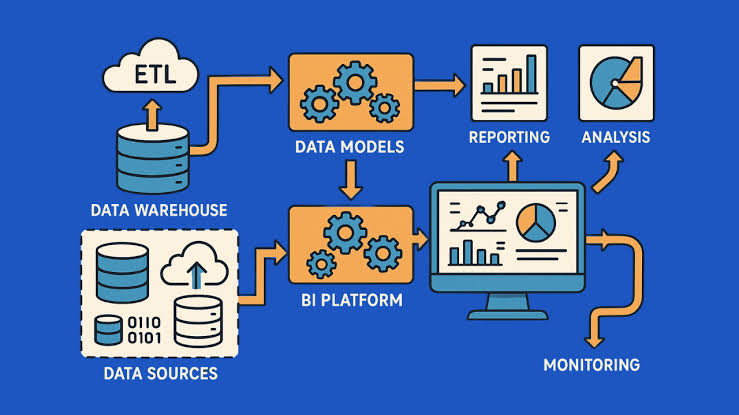
\includegraphics[width=0.6\textwidth]{architecture_bi.png}
\caption{Architecture of a Business Intelligence system \cite{chaudhuri2011}}
\label{fig:architecture_bi_atb}
\end{figure}

The detailed structure of such a system comprises the following elements:

\begin{itemize}
    \item \textbf{Data sources}: heterogeneous operational data generated inside and outside
    the organisation.
    \item \textbf{ETL/ELT process}: extracts, optionally transforms, and loads data into a
    centralised repository.
    \item \textbf{Operational Data Store (ODS)}: intermediate staging area between operational
    sources and the data warehouse.
    \item \textbf{Data Warehouse}: centralised database organising structured data for
    analytical queries.
    \item \textbf{Data Marts}: domain-specific subsets of the warehouse.
    \item \textbf{Analytical layer}: OLAP cubes, ML models, and reporting tools.
    \item \textbf{Visualisation}: dashboards and reports for business decision-makers.
\end{itemize}


%----------------------------------------------
\subsection{ETL and ELT Paradigms}
%----------------------------------------------

Data integration is the backbone of any decision-support system. Rahm and Do \cite{rahm2000}
formalise the data quality challenges encountered during extraction, transformation, and
loading: schema heterogeneity, null handling, encoding inconsistencies, and duplicate
records. Two main integration paradigms exist:

\begin{table}[H]
\centering
\caption{Comparative analysis of ETL versus ELT}
\label{tab:atb_etl_elt}
\begin{tabular}{|p{3cm}|p{5cm}|p{5cm}|}
\hline
\rowcolor{blue!15}
\textbf{Aspect} & \textbf{ETL} & \textbf{ELT} \\
\hline
Maturity & Mature, widely adopted & Emerging cloud-native pattern \\
\hline
Data type & Structured operational data & Structured and semi-structured data \\
\hline
Transformation location & Outside the warehouse & Inside the database engine \\
\hline
Traceability & External transformation scripts & Versioned SQL models (e.g., dbt) \\
\hline
Typical use & Traditional BI, on-premise DWH & Data Lakes, Cloud, modern DWH \\
\hline
\end{tabular}
\end{table}

The ATB project follows an \textbf{ELT-oriented architecture}: data from seven
pipe-separated CSV files is first loaded into the SQL Server ODS schema
(\texttt{PFE\_ODS}), then transformed using versioned dbt SQL models inside the database.
This choice aligns with Kimball's recommendation \cite{kimball2013} to perform
transformations as close to the analytical store as possible, enabling full lineage tracking
and reproducibility.

The transformation layer is divided into three levels:

\begin{itemize}
    \item \textbf{Staging}: cleans raw ODS data, casts types, standardises names,
    and preserves source truth.
    \item \textbf{Intermediate}: applies business logic, joins reference data, computes
    account aggregates, and calculates the three-pillar risk scores.
    \item \textbf{Warehouse}: builds conformed dimensions and fact tables for BI, ML,
    and reporting.
\end{itemize}

%----------------------------------------------
\subsection{Data Warehouse, Data Lake, and Data Mart}
%----------------------------------------------

The choice of the appropriate data storage paradigm is a critical architectural decision in
any decision-support system. Three complementary concepts are defined in the literature:
the Data Warehouse, the Data Lake, and the Data Mart. Understanding their differences allows
an informed selection based on the nature of the data, the analytical requirements, and the
technical maturity of the organisation \cite{kimball2013, inmon2005}.

\textbf{(1) Data Warehouse (DWH)}

A Data Warehouse (DWH) is a centralised, subject-oriented, integrated, non-volatile, and
time-variant data repository designed to support analytical queries and decision-making at
the enterprise level \cite{inmon2005}. Inmon's definition emphasises four key properties:

\begin{itemize}
    \item \textbf{Subject-oriented}: organised around business subjects (customers, accounts,
    risk) rather than operational transactions.
    \item \textbf{Integrated}: data from heterogeneous sources is harmonised into a single
    consistent schema.
    \item \textbf{Non-volatile}: once written, records are not modified or deleted; history
    is preserved.
    \item \textbf{Time-variant}: each record carries a temporal reference, enabling
    historical analysis and trend monitoring.
\end{itemize}

Kimball \cite{kimball2013} extends this definition by proposing the dimensional modelling
approach: data is organised around fact tables (quantitative measurements) and dimension
tables (analytical context), forming star, snowflake, or constellation schemas optimised
for analytical query performance.

\textbf{(2) Data Lake}

A Data Lake is a large-scale, schema-on-read storage repository that ingests raw data in
its original format---structured, semi-structured, or unstructured---and defers the
application of structure until query time \cite{kimball2013}. Unlike a Data Warehouse, a
Data Lake does not impose a predefined schema on ingestion, making it flexible for storing
diverse data types (logs, JSON, images, streams). However, without governance, a Data Lake
can degrade into a ``Data Swamp'' where data is stored but not usable.

The key differences between a Data Lake and a Data Warehouse are:

\begin{itemize}
    \item \textbf{Schema}: schema-on-read (Data Lake) versus schema-on-write (Data Warehouse).
    \item \textbf{Data type}: any format (Data Lake) versus structured only (Data Warehouse).
    \item \textbf{Target user}: data scientists exploring raw data (Data Lake) versus
    business analysts querying governed KPIs (Data Warehouse).
    \item \textbf{Performance}: flexible but slower for aggregated queries (Data Lake) versus
    optimised for analytical workloads (Data Warehouse).
\end{itemize}

\textbf{(3) Data Mart}

A Data Mart is a domain-specific, scoped subset of a Data Warehouse, tailored to the
analytical needs of a specific business unit or subject area \cite{inmon2005}. It is smaller
than a full enterprise warehouse and faster to query for its focused domain. Data Marts
can be dependent (derived from a central DWH) or independent. The bottom-up Kimball
approach builds the enterprise warehouse progressively through interconnected Data Marts
sharing conformed dimensions.

\begin{table}[H]
\centering
\small
\renewcommand{\arraystretch}{1.4}
\caption{Comparison: Data Warehouse, Data Lake, and Data Mart}
\label{tab:dwh_lake_mart}
\begin{tabular}{|p{3cm}|p{3.7cm}|p{3.7cm}|p{3.7cm}|}
\hline
\rowcolor{blue!15}
\textbf{Criterion} & \textbf{Data Warehouse} & \textbf{Data Lake} & \textbf{Data Mart} \\
\hline
Data type & Structured, governed & Any (raw, unstructured) & Structured, domain-scoped \\
\hline
Schema & Schema-on-write & Schema-on-read & Schema-on-write \\
\hline
Scope & Enterprise-wide & Organisation-wide & Business unit or subject \\
\hline
Users & Business analysts, BI tools & Data scientists, engineers & Domain analysts \\
\hline
Query performance & High (optimised) & Lower (flexible) & Very high (focused) \\
\hline
Complexity & High & Medium (governance risk) & Low \\
\hline
Example technology & SQL Server, Oracle DWH & AWS S3, Azure Data Lake & PostgreSQL subject mart \\
\hline
\end{tabular}
\end{table}

%----------------------------------------------
\subsection{Multidimensional Modelling}
%----------------------------------------------

In multidimensional modelling, a schema is composed of a central \textbf{fact table} and
\textbf{dimension tables} \cite{kimball2013}. Three standard schema types are defined in
the literature:

\textbf{(1) Star Schema}

A star schema contains one central fact table surrounded by denormalised dimensions,
forming a structure resembling a star. It is simple and performant for BI dashboards.

\begin{figure}[H]
\centering
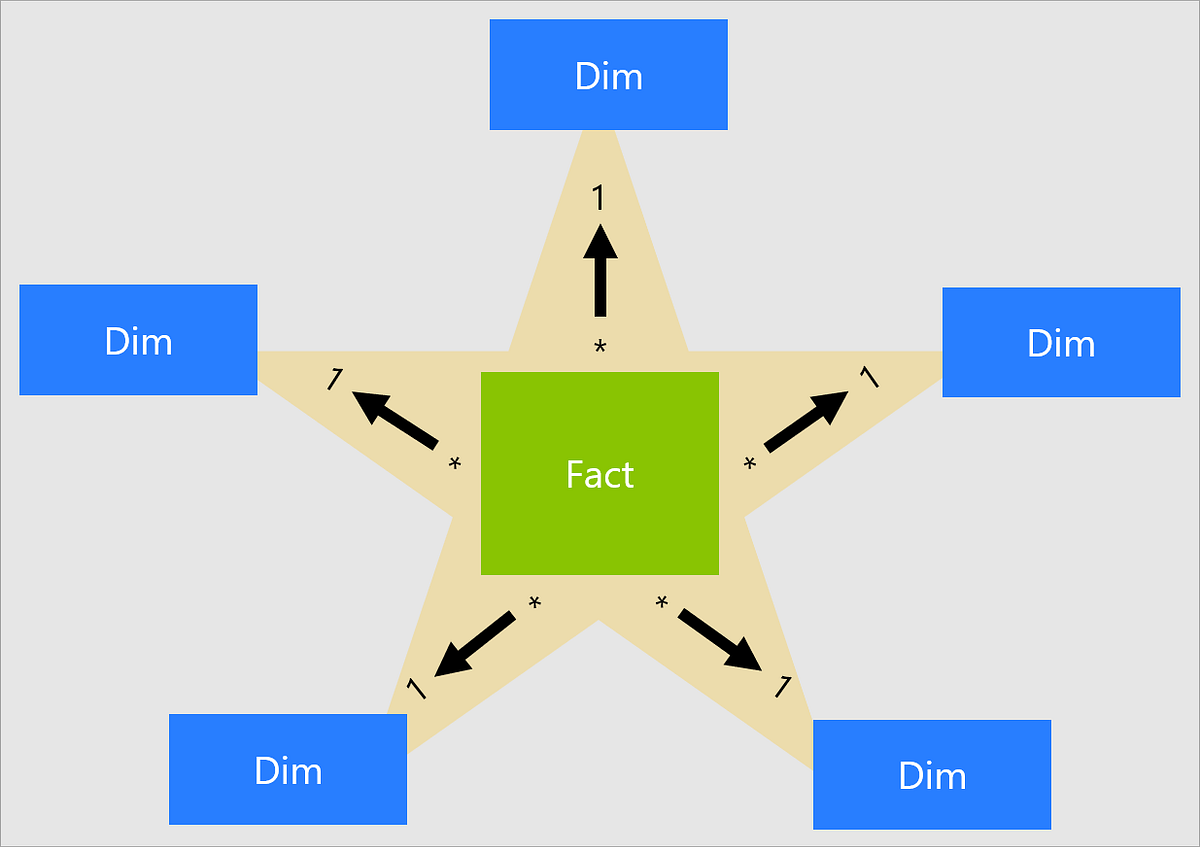
\includegraphics[width=0.4\textwidth]{star_schema.png}
\caption{Star schema dimensional modelling \cite{kimball2013}}
\label{fig:star_schema_atb}
\end{figure}

\textbf{(2) Snowflake Schema}

A snowflake schema normalises dimension tables into subdimensions. It can reduce redundancy
but increases join complexity \cite{inmon2005}.

\begin{figure}[H]
\centering
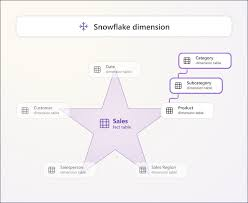
\includegraphics[width=0.4\textwidth]{snowflake_schema.png}
\caption{Snowflake schema dimensional modelling \cite{inmon2005}}
\label{fig:snowflake_schema_atb}
\end{figure}

\textbf{(3) Constellation Schema (Galaxy Schema)}

A constellation schema contains several fact tables sharing conformed dimensions. This is
the \textbf{selected model} for the ATB project, as it supports both account-level analytics
and customer risk analytics through two independent fact tables that share common dimensions
\cite{kimball2013}.

\begin{figure}[H]
\centering
\includegraphics[width=0.5\textwidth]{galaxy_schema.png}
\caption{Constellation (galaxy) schema dimensional modelling \cite{kimball2013}}
\label{fig:galaxy_schema_atb}
\end{figure}

\begin{table}[H]
\centering
\small
\caption{ATB constellation warehouse structure}
\label{tab:atb_constellation}
\begin{tabular}{|p{4cm}|p{4.5cm}|p{5cm}|}
\hline
\rowcolor{blue!15}
\textbf{Component} & \textbf{Grain} & \textbf{Purpose} \\
\hline
\textbf{fact\_account} & One row per account snapshot & Descriptive analytics: balance,
overdraft flag, credit balance, account age. \\
\hline
\textbf{fact\_customer\_risk} & One row per customer per scoring date & Risk analytics:
CRI, FFS, BRS, global risk score, risk tier. \\
\hline
\textbf{Shared dimensions} & Customer, DAO, sector, industry, target, date & Common
analytical context for both facts. \\
\hline
\textbf{Specific dimensions} & Currency, risk profile & Currency (accounts); risk profile
(customer risk). \\
\hline
\end{tabular}
\end{table}

The ATB warehouse contains 8 dimensions and 2 fact tables (281,960 total rows,
0 null foreign keys).

%----------------------------------------------
\subsection{Data Warehouse Design Approaches}
%----------------------------------------------

\textbf{(1) Bottom-Up Approach (Kimball)}

Initiated by Ralph Kimball \cite{kimball2013}, this approach builds the warehouse
progressively through dimensional data marts connected by conformed dimensions. It is
particularly suited to BI projects requiring early dashboard delivery and business-readable
models.

\begin{figure}[H]
\centering
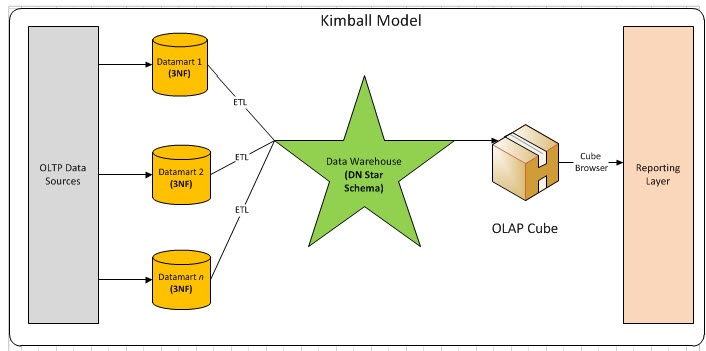
\includegraphics[width=0.65\textwidth]{kimball_model.png}
\caption{Bottom-up approach according to Ralph Kimball \cite{kimball2013}}
\label{fig:kimball_atb}
\end{figure}

The ATB project follows a Kimball-oriented approach: conformed dimensions are built first,
then fact tables for account analytics and customer risk analytics.

\textbf{(2) Top-Down Approach (Inmon)}

Initiated by Bill Inmon \cite{inmon2005}, this approach begins with a centralised enterprise
data warehouse before deriving specialised data marts. It requires more upfront modelling
effort but maintains stronger enterprise-level consistency.

\begin{figure}[H]
\centering
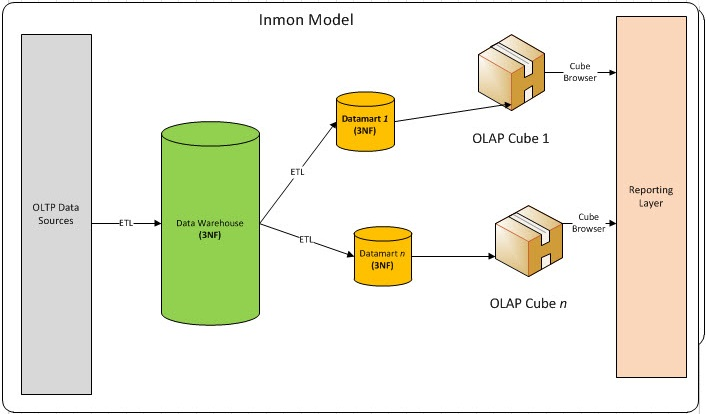
\includegraphics[width=0.65\textwidth]{inmon_model.png}
\caption{Top-down approach according to Bill Inmon \cite{inmon2005}}
\label{fig:inmon_atb}
\end{figure}

\textbf{(3) Hybrid Approach}

A hybrid approach combines enterprise consistency with incremental delivery
\cite{kimball2013, inmon2005}. The ATB project can be considered hybrid in practice
because it uses a central SQL Server warehouse while delivering domain-focused facts for
account analytics and risk analytics independently.

\begin{figure}[H]
\centering
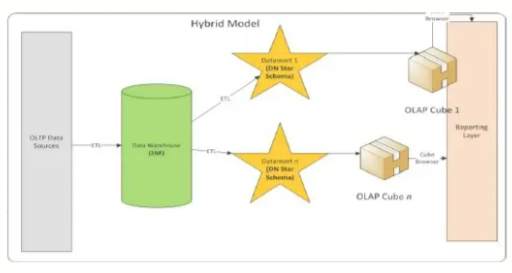
\includegraphics[width=0.65\textwidth]{hybrid_model.png}
\caption{Hybrid data warehouse approach (Inmon + Kimball) \cite{kimball2013, inmon2005}}
\label{fig:hybrid_atb}
\end{figure}

%----------------------------------------------
\subsection{Key Performance Indicators (KPI)}
%----------------------------------------------

KPIs constitute the common language between technical data processing and business
decision-making. According to Eckerson \cite{eckerson2010}, a good BI dashboard must
integrate three types of indicators:

\begin{itemize}
    \item \textbf{Strategic KPIs}: global view of portfolio and risk performance.
    \item \textbf{Operational KPIs}: daily monitoring of accounts, compliance alerts, and
    branch activity.
    \item \textbf{Leading KPIs}: predictive signals from ML scores and drift monitoring.
\end{itemize}

\begin{table}[H]
\centering
\small
\caption{Main KPI families of the ATB BI platform}
\label{tab:atb_kpis}
\begin{tabular}{|p{4cm}|p{5cm}|p{4.2cm}|}
\hline
\rowcolor{blue!15}
\textbf{KPI family} & \textbf{Examples} & \textbf{Business value} \\
\hline
Customer portfolio & Total customers, distribution by employment, sector, gender, branch. &
Understand the structure of the customer base. \\
\hline
Account analytics & Total accounts, total working balance, average balance, overdraft rate,
account age. & Monitor financial portfolio health. \\
\hline
Risk and compliance & Global risk score, risk tier distribution, KYC completeness, PEP count,
compliance flags. & Prioritise controls and compliance actions. \\
\hline
ML performance & Accuracy, F1-score, ROC-AUC, PR-AUC, Brier score. &
Monitor model quality and predictive reliability. \\
\hline
Data quality & Row counts, null foreign keys, referential integrity, freshness timestamps. &
Guarantee trustworthy dashboard outputs. \\
\hline
\end{tabular}
\end{table}

%----------------------------------------------
\subsection{Foundational Works on Banking Risk Scoring}
%----------------------------------------------

The ATB composite risk score is grounded in four foundational references from the
scientific literature:

\textbf{(1) Regulatory compliance as a first-order risk driver.}
The FATF Recommendations \cite{fatf2012} establish that incomplete KYC data, PEP exposure,
and compliance flags must be treated as primary risk signals before any financial analysis.
This justifies dedicating the highest pillar weight (40\%) to the Compliance Risk Index.

\textbf{(2) Financial fragility as a credit-scoring predictor.}
Lessmann et al.\ \cite{lessmann2015} demonstrate through a large-scale classification
benchmark that financial variables---salary, balance levels, and overdraft behaviour---are
the strongest predictors of financial vulnerability. This supports the Financial Fragility
Score as the second pillar (35\%).

\textbf{(3) Behavioural patterns as complementary signals.}
Hand and Henley \cite{hand1997} show that consumer credit scoring benefits from behavioural
indicators (account tenure, payment history, activity patterns) complementing pure financial
ratios. The Behavioural Risk Score (25\%) captures customer tenure, negative balances, and
KYC staleness.

\textbf{(4) Multi-pillar aggregation.}
The Basel~III framework \cite{bcbs2011} formalises that bank risk must be assessed through
complementary pillars aggregated into a single supervisory view. Eckerson \cite{eckerson2010}
extends this logic to BI dashboards via weighted composite KPIs.



%================================================
\section{MLOps and Traceability: MLflow}
%================================================

%----------------------------------------------
\subsection{Challenges of Machine Learning in Production}
%----------------------------------------------

Sculley et al.\ \cite{sculley2015} formalised the concept of technical debt in production
ML systems, identifying three structural challenges:

\begin{enumerate}
    \item \textbf{Reproducibility}: a model trained today must be reproducible with the
    same code, data preparation logic, parameters, and random seed.
    \item \textbf{Traceability}: every experiment must preserve its full context
    (parameters, metrics, artefacts, data version).
    \item \textbf{Comparability}: performance across model versions must be directly
    comparable to enable data-driven model selection.
\end{enumerate}

These challenges are amplified in a banking context where model outputs must be
auditable, explainable, and reproducible for regulatory compliance.

%----------------------------------------------
\subsection{MLflow: Architecture and Components}
%----------------------------------------------

MLflow, developed by Databricks \cite{zaharia2018}, has become the reference platform for
managing the machine learning development lifecycle. To justify this choice, a comparative
analysis of the leading MLOps platforms is presented in Table~\ref{tab:mlops-comparison}.

\begin{table}[H]
\centering
\caption{Comparison of main MLOps platforms}
\label{tab:mlops-comparison}
\begin{tabular}{|l|c|c|c|c|}
\hline
\rowcolor{blue!15}
\textbf{Platform} & \textbf{Tracking} & \textbf{Versioning} & \textbf{Deployment} &
\textbf{Open Source} \\
\hline
MLflow & ++ & ++ & + & \checkmark \\
Kubeflow & + & + & ++ & \checkmark \\
Weights \& Biases & +++ & + & + & Freemium \\
Neptune & ++ & + & + & Freemium \\
\hline
\end{tabular}
\caption*{\small Legend: + (basic support), ++ (advanced support), +++ (exceptional support)}
\end{table}

MLflow provides four core components:

\begin{enumerate}
    \item \textbf{MLflow Tracking}: logs runs, hyperparameters, metrics, thresholds, and
    artefacts for experiment comparison.
    \item \textbf{MLflow Projects}: standardises execution environments for reproducibility.
    \item \textbf{MLflow Models}: packages serialised classifiers as versioned artefacts.
    \item \textbf{MLflow Registry}: manages the model lifecycle (Staging, Production,
    Archived) with audit trails.
\end{enumerate}

\begin{figure}[H]
\centering
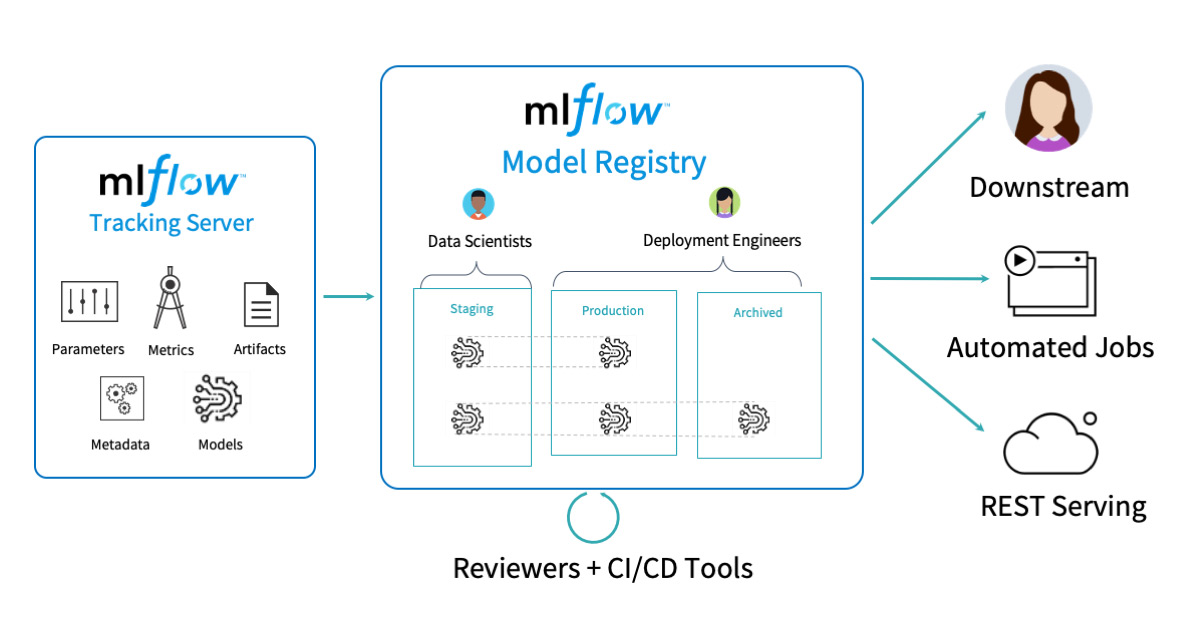
\includegraphics[width=0.8\textwidth]{figures/mlflow_architecture.jpg}
\caption{Architecture de MLflow avec backend SQLite\cite{mlflow_architecture}}
\label{fig:mlflow_architecture}
\end{figure}


%================================================
\section{Generative AI for Dashboard Explanation}
%================================================

%----------------------------------------------
\subsection{Large Language Models (LLMs) in Business Intelligence}
%----------------------------------------------

The emergence of Large Language Models (LLMs) has transformed data interaction paradigms.
In the context of Business Intelligence and analytical reporting, recent studies \cite{baidoo2023}
identify three primary use-cases for LLMs:
\begin{enumerate}
    \item \textbf{Narrative generation}: Translating complex structured reports into accessible text summaries.
    \item \textbf{Intelligent query assistants}: Allowing users to query databases using natural language.
    \item \textbf{Explaining machine learning outputs}: Translating predictions, tree weights, and feature attributions (e.g., SHAP values) into plain corporate language.
\end{enumerate}

%----------------------------------------------
\subsection{Google Gemini for Chart Narration}
%----------------------------------------------

Google Gemini, developed by Google DeepMind \cite{gemini2024}, is a family of multimodal
models optimized for large token contexts, low latency, and advanced reasoning. In this
project, \texttt{gemini-2.0-flash} is used as the sole generative engine for on-demand
chart explanations: a statistical summary of the visible Plotly figure is sent to the
API, which returns a short, role-aware paragraph for banking users.

%----------------------------------------------
\subsection{Availability and Local Template Fallback}
%----------------------------------------------

A practical challenge when calling a commercial LLM API from an operational dashboard is
service availability: rate limits, network issues or a missing API key must not break the
BI application. The ATB platform therefore pairs Gemini with a \textbf{deterministic local
template fallback}: if the API call fails or no key is configured, a pre-authored
explanation sentence is shown instead. This keeps the ``Explain chart'' feature always
usable without introducing a second LLM provider.



%================================================
\section{Data Application Development Frameworks}
%================================================

%----------------------------------------------
\subsection{Streamlit for BI and ML Deployment}
%----------------------------------------------

Bhatt et al.\ \cite{bhatt2021} evaluate the principal Python dashboard frameworks for
data science applications. The ATB project uses Streamlit as the primary operational
dashboard framework, complemented by Jupyter Notebooks for ML development and exploration.

\begin{table}[H]
\centering
\footnotesize
\caption{Comparison of data application frameworks}
\label{tab:atb_reporting_frameworks}
\begin{tabular}{|p{2.8cm}|p{2.4cm}|p{2.4cm}|p{2.4cm}|p{2.4cm}|}
\hline
\rowcolor{blue!15}
\textbf{Criterion} & \textbf{Streamlit} & \textbf{Jupyter} & \textbf{Dash} &
\textbf{Power BI} \\
\hline
Learning curve & Very low & Low & Medium & Medium \\
\hline
ML integration & Excellent & Native & Good & Limited \\
\hline
Role-based pages & In code (RBAC) & Not designed & Custom & Workspace \\
\hline
Banking logic & Full Python & Full Python & Full Python & DAX/M \\
\hline
Interactivity & Native & Via widgets & JavaScript & Native \\
\hline
Project usage & \textbf{Selected} & ML \& EDA & Compared & Compared Ch.~1 \\
\hline
\end{tabular}
\end{table}

The Streamlit dashboard implements role-based navigation for General Management, Chief
Compliance, and Branch Manager profiles, with pages covering executive overview, BI
studies, compliance monitoring, alerts, risk analysis, accounts, MLflow tracking, ML
risk model, and data explorer.


%================================================
\section{Synthesis and Positioning}
%================================================

The state-of-the-art analysis shows that the ATB BI project is positioned at the
intersection of three mature domains: Business Intelligence, data warehousing, and machine
learning. Its scientific added value comes from integrating these domains into a single,
governed, operational banking platform.

Many BI projects stop at descriptive dashboards. Conversely, many ML prototypes remain
disconnected from governed data models and operational reporting. The ATB project addresses
this gap by building a complete, reproducible pipeline: CSV ingestion into SQL Server via
Airbyte and Python, dbt transformations across three layers, a Kimball-style constellation
warehouse with 8 dimensions and 281,960 total rows, Airflow orchestration, MLflow tracking
for full model traceability, SHAP explainability for interpretable audit-grade predictions,
and Streamlit dashboards for banking decision-makers.

The project therefore transforms raw banking data into a governed decision-support platform
capable of descriptive analytics, risk monitoring, predictive classification, and explainable
reporting for ATB stakeholders.


%================================================
\section{Requirements Specification}
%================================================

Requirements specification is a pivotal step in software engineering. It establishes a
clear contract between the banking business needs of the ATB and the technical solution to
be developed, while delimiting the functional scope of the platform.

%----------------------------------------------
\subsection{Actor Identification}
%----------------------------------------------

An actor represents the abstraction of a role played by a human or external system
interacting with the platform. In the ATB system, the following actors have been
identified, each with distinct access rights based on Role-Based Access Control (RBAC):

\begin{itemize}
    \item \textbf{General Management (DG\_CENTRAL)}: accesses executive KPIs, portfolio
    summaries, risk distribution, and high-level monitoring pages.
    \item \textbf{Chief Compliance Officer (CHEF\_CONFORMITE)}: monitors KYC completeness,
    PEP customers, compliance flags, alerts, and customer watchlists.
    \item \textbf{Branch Manager (CHEF\_AGENCE)}: analyses customers and accounts scoped to
    a specific DAO area or branch perimeter.
\end{itemize}

%----------------------------------------------
\subsection{Functional Requirements}
%----------------------------------------------

Functional requirements describe the actions the system must be able to execute in order to
satisfy the business stakeholders. They are categorised by actor role and analytical domain:

\textbf{1. General Management Dashboard Module}
\begin{itemize}
    \item The system must display executive KPI summaries: total customers, total accounts,
    global risk distribution, and portfolio structure.
    \item The system must provide portfolio overview charts by sector, industry, nationality,
    gender, and employment status.
    \item The system must allow export of executive summaries and KPI snapshots to CSV.
    \item The system must display AI-generated plain-language explanations of complex charts.
\end{itemize}

\textbf{2. Compliance and Risk Monitoring Module}
\begin{itemize}
    \item The system must display KYC completeness rates and flag customers with missing
    KYC records.
    \item The system must list PEP customers with associated risk scores and compliance
    alert status.
    \item The system must display risk tier distribution (LOW, MEDIUM, HIGH, VERY\_HIGH)
    with drill-down by branch or DAO area.
    \item The system must provide a compliance alert watchlist with filtering and export
    to CSV.
    \item The system must visualise the three-pillar risk score decomposition (CRI, FFS,
    BRS) per customer or segment.
\end{itemize}

\textbf{3. Branch Analytics Module}
\begin{itemize}
    \item The system must filter all dashboard views to the DAO area or branch scope
    assigned to the Branch Manager.
    \item The system must display account activity metrics: working balance, overdraft rate,
    account age, and credit balance for the managed perimeter.
    \item The system must allow comparison of branch performance against the global
    portfolio benchmark.
    \item The system must provide customer-level drill-down within the managed branch perimeter.
\end{itemize}

\textbf{4. Machine Learning and Predictive Analytics Module}
\begin{itemize}
    \item The system must expose XGBoost risk predictions for all customers in a dedicated
    ML dashboard page.
    \item The system must display SHAP feature importance plots for model interpretability.
    \item The system must provide MLflow experiment tracking data (metrics, parameters,
    artefacts) in a dedicated MLflow page.
    \item The system must allow on-demand batch scoring and write results to the
    \texttt{PFE\_ML} schema.
\end{itemize}

%----------------------------------------------
\subsection{Non-Functional Requirements}
%----------------------------------------------

Non-functional requirements define quality, performance, confidentiality, and maintainability
constraints that the architectural design must satisfy:

\begin{itemize}
    \item \textbf{Data quality}: fact tables must have 0 null foreign keys, valid referential
    integrity, controlled row counts, and freshness timestamps.
    \item \textbf{Performance}: the daily warehouse pipeline must complete within
    approximately 35 minutes, with optional ML retraining triggered as a downstream batch step.
    \item \textbf{Traceability}: dbt models, Airflow DAGs, ML runs, model metrics, and
    artefacts must be versioned and auditable through MLflow.
    \item \textbf{Confidentiality}: access to customer data, risk scores, and compliance
    information must be restricted to authorised roles only through RBAC; data must remain
    within ATB's internal infrastructure.
    \item \textbf{Availability}: the daily pipeline must be monitored with Airflow retry
    mechanisms and alerting to ensure consistent data freshness for morning dashboard sessions.
    \item \textbf{Maintainability}: the project must remain modular through separation of
    the five implementation folders.
    \item \textbf{Explainability}: risk scores must be interpretable through three business
    pillars, and model behaviour must be explained through SHAP artefacts.
    \item \textbf{Usability}: dashboards must provide readable KPIs, clear navigation,
    consistent colours, and business-oriented explanations.
\end{itemize}

%----------------------------------------------
\subsection{Architectural View of Use Cases}
%----------------------------------------------

In order to formalise the interactions between actors and the system, the functional
requirements are modelled through a global use case diagram.
\begin{figure}[H]
\centering
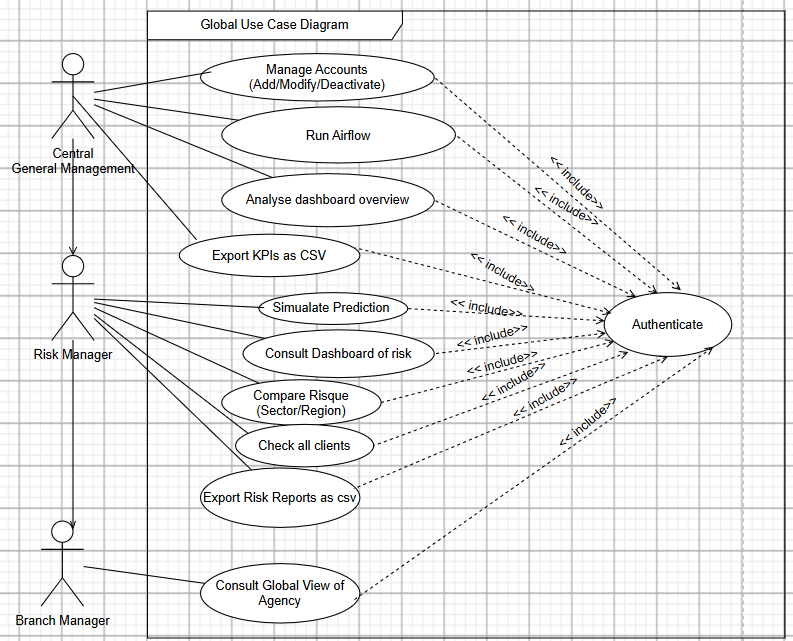
\includegraphics[width=0.9\textwidth]{figures/GlobalUseCaseDiagram.png}
\caption{Global Use case diagram\cite{atb_use_case_global}}
\label{fig:uc_sprint1}
\label{fig:atb_use_case_global}
\end{figure}

%================================================
\section{Project Planning}
%================================================

%----------------------------------------------
\subsection{Team and Roles}
%----------------------------------------------

The Scrum methodology having been adopted as detailed in Chapter~1, this section presents
the project team organisation for the ATB BI platform.

\begin{table}[H]
\centering
\caption{Scrum team organisation for the ATB BI platform}
\label{tab:atb_project_roles}
\begin{tabular}{|p{3.5cm}|p{3.8cm}|p{6.2cm}|}
\hline
\rowcolor{blue!15}
\textbf{Scrum Role} & \textbf{Assigned to} & \textbf{Responsibility} \\
\hline
Product Owner & ATB Administration (\textit{Direction March\'{e} Entreprises}) &
Represents business needs; prioritises the backlog; validates KPIs, risk views,
dashboard scope, and compliance requirements. \\
\hline
Scrum Master & M. Mouhamed Saddek Snoussi & Facilitates Scrum ceremonies, follows sprint
progress, removes blockers, and ensures alignment between the team and ATB stakeholders. \\
\hline
Development Team & Ahmed El Abed & Implements the platform end-to-end: ingestion, SQL
Server schemas, dbt models, Airflow DAGs, ML training (XGBoost and Random Forest), MLflow,
and Streamlit dashboards. \\
\hline
\end{tabular}
\end{table}

%----------------------------------------------
\subsection{Three-Tier Software Architecture}
\label{sec:atb_three_tier_architecture}
%----------------------------------------------

To ensure the modularity, maintainability, and scalability of the ATB platform, a
\textbf{three-tier software architecture} is adopted. This proven design pattern separates
the application into three distinct logical layers:

\begin{figure}[H]
\centering
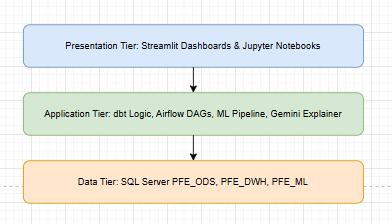
\includegraphics[width=0.75\textwidth]{atb_three_tier_architecture.png}
\caption{Three-tier software architecture of the ATB BI platform}
\label{fig:atb_three_tier_architecture}
\end{figure}

\textbf{1.~The Presentation Tier}: the Streamlit dashboard. Displays KPIs, interactive
charts, risk tables, model metrics, alerts, role-based pages, and AI-generated chart
explanations for ATB business users.

\textbf{2.~The Application Tier}: all processing and business logic. Includes Airflow DAGs
for daily scheduling, dbt transformation models (staging, intermediate, warehouse), risk
scoring SQL logic, Python ML scripts (XGBoost), MLflow integration, SHAP
explainability, and Gemini explanation calls.

\textbf{3.~The Data Tier}: persistent storage in SQL Server using three schemas:
\texttt{PFE\_ODS} for raw operational data (7 source tables), \texttt{PFE\_DWH} for the
constellation warehouse (8 dimensions, 2 fact tables, 281,960 total rows, 0 null foreign
keys), and \texttt{PFE\_ML} for ML prediction outputs.
%----------------------------------------------
\subsection{Product Backlog}
%----------------------------------------------

The product backlog groups all User Stories of the project, formulated according to the
Scrum standard. Each User Story is written from the perspective of one of the three
identified system actors, translating a concrete business need into a prioritised
functionality.

\begin{table}[H]
\centering
\caption{Product Backlog (Final Version - Streamlit \& AI)}
\label{tab:atb_product_backlog}

\small
\renewcommand{\arraystretch}{1.4}

\begin{tabularx}{\textwidth}{|c|c|c|X|}
\hline
\rowcolor{blue!15}
\textbf{US} & \textbf{Priority} & \textbf{Sprint} & \textbf{Description} \\
\hline

US 01 & Low & Sprint 1 &
As All Actors, I want to authenticate securely to access the platform. \\
\hline

US 02 & Medium & Sprint 1 &
As Central General Management, I want to create, modify, activate or deactivate accounts for branch and risk managers. \\
\hline

US 03 & Very High & Sprint 2 &
As Central General Management, I want to orchestrate the entire application automatically  with Airflow. \\
\hline

US 04 & High & Sprint 3 &
As Central General Management, I want to extract and load via Airbyte. \\
\hline

US 05 & High & Sprint 3 &
As Central General Management, I want to define and calculate risk KPIs in the central data warehouse. \\
\hline

US 06 & High & Sprint 3 &
As Branch Manager, I want to consult my agency's filtered view on Streamlit to monitor my activity. \\
\hline

US 07 & High & Sprint 3 &
As Central General Management, I want to analyze indicators for all agencies at the national level on Streamlit. \\
\hline

US 08 & High & Sprint 3 &
As Central General Management, I want to export and download management indicators as CSV files. \\
\hline

US 09 & Low & Sprint 3 &
As Risk Manager, I want to track the history and evolution of customers across all agencies. \\
\hline

US 10 & High & Sprint 4 &
As Risk Manager, I want to train the Artificial Intelligence algorithm to detect future defaults. \\
\hline

US 11 & High & Sprint 4 &
As Risk Manager, I want to consult the Artificial Intelligence predictions. \\
\hline

US 12 & High & Sprint 4 &
As Risk Manager, I want to read the automatic (AI-generated) interpretation of curves and the risk matrix on Streamlit. \\
\hline

US 13 & High & Sprint 4 &
As Risk Manager, I want to mathematically compare risk levels by sector and by geographic zone. \\
\hline

US 14 & High & Sprint 4 &
As Risk Manager, I want to download predictive customer scores (CSV) for other external tools. \\
\hline

\end{tabularx}
\end{table}

\clearpage
%----------------------------------------------
\subsection{Delivery Process (Releases)}
%----------------------------------------------

The project is structured into \textbf{3 Releases} covering \textbf{4 Sprints} of three
weeks each, consistent with the Gantt chart defined in Chapter~1.
Table~\ref{tab:atb_releases_plan} summarises how each release maps to sprints,
methodologies and user stories.

\begin{table}[!ht]
\centering
\caption{Delivery strategy: Releases, Sprints, and User Stories}
\label{tab:atb_releases_plan}
\renewcommand{\arraystretch}{1.35}
\footnotesize
\resizebox{\textwidth}{!}{
\begin{tabular}{|c|c|p{4.0cm}|p{7.0cm}|}
\hline
\rowcolor{blue!15}
\textbf{Release} & \textbf{Sprint(s)} & \textbf{Theme} & \textbf{User Stories} \\
\hline

\textbf{Release 1}
& \textbf{Sprint 1 \& 2}
& \textbf{Application \& \newline Engine}
&
\textbf{Sprint 1:} \newline
\textbf{US 01} : Authenticate securely to access the platform \newline
\textbf{US 02} : Create, modify, activate or deactivate accounts for branch and risk managers \newline
\textbf{Sprint 2:} \newline
\textbf{US 03} : Orchestrate the entire application automatically each night with Airflow \\
\hline

\textbf{Release 2}
& \textbf{Sprint 3}
& \textbf{Business \newline Intelligence (BI)}
&
\textbf{US 04} : Extract and load source files via Airbyte \newline
\textbf{US 05} : Define and calculate risk KPIs in the central data warehouse \newline
\textbf{US 06} : Consult my agency's filtered view on Streamlit to monitor my activity \newline
\textbf{US 07} : Analyze indicators for all agencies at the national level on Streamlit \newline
\textbf{US 08} : Export and download management indicators as CSV files \newline
\textbf{US 09} : Track the history and evolution of customers across all agencies \\
\hline

\textbf{Release 3}
& \textbf{Sprint 4}
& \textbf{Artificial \newline Intelligence (ML)}
&
\textbf{US 10} : Train the Machine learning algorithm to detect future defaults \newline
\textbf{US 11} : Consult the Machine learning predictions. \newline
\textbf{US 12} : Read the automatic (AI-generated) interpretation of curves and the risk matrix on Streamlit \newline
\textbf{US 13} : Mathematically compare risk levels by sector and by geographic zone \newline
\textbf{US 14} : Download predictive customer scores (CSV) for other external tools \\
\hline

\end{tabular}
}
\end{table}


%================================================
\section{Work Environment and Tools}
%================================================

The implementation of a banking BI and ML platform requires a stable technical environment
and a coherent technology stack.

%----------------------------------------------

\subsection{Hardware Environment}

The development, testing, transformation, dashboarding, and local ML training were performed
on a workstation with the following characteristics:

\begin{itemize}
    \item \textbf{Product Name}: MSI GF63 Thin 10SCXR
    \item \textbf{Operating System}: Microsoft Windows 10 Professionnel 64-bit (OS build 19045.6466)
    \item \textbf{BIOS Version}: E16R4IMS.107 (Release Date: 2020/05/28)
    \item \textbf{Processor}: Intel(R) Core(TM) i7-10750H CPU @ 2.60\,GHz
    \item \textbf{Memory (RAM)}: 16\,GB DDR4-2667 (Crucial CT16G4SFD8266.C16FD1) @ 1333\,MHz
    \item \textbf{Graphics}: NVIDIA GeForce GTX 1650 with Max-Q Design (4095\,MB) and Intel(R) UHD Graphics (1024\,MB)
\end{itemize}

\begin{figure}[H]
\centering

\includegraphics[height=1.8cm, keepaspectratio]{msi_logo.png}
\caption{MSI Logo\cite{msi_logo_atb}}
\label{fig:msi_logo_atb}
\end{figure}

This configuration provides sufficient CPU parallelism for dbt transformations, local four-model
ML training, Docker-based Airflow execution, and Streamlit dashboard development.


\subsection{Design and Development Tools}

\subsubsection{Visual design tools}

Architecture diagrams, warehouse models, UML use case diagrams, and report figures were designed
using \textbf{Draw.io} (diagrams.net) \cite{drawio}. This open-source tool is appropriate for
UML diagrams, BI architecture diagrams, and data flow representations. The editable source file for all the diagrams.

\begin{figure}[H]
\centering

\includegraphics[height=1.5cm, keepaspectratio]{drawio_logo.png}
\caption{Draw.io logo\cite{drawio}}
\label{fig:drawio_logo_atb}
\end{figure}

\subsubsection{Integrated development environment}

The codebase is organised and edited using \textbf{Visual Studio Code (VS Code)} \cite{vscode}.
It is suitable for Python development, SQL and dbt modelling, Airflow DAG editing, Markdown
documentation, and Git-based project organisation.

\begin{figure}[H]
\centering

\includegraphics[height=1.5cm, keepaspectratio]{vscode_logo.png}
\caption{Visual Studio Code logo\cite{vscode}}
\label{fig:vscode_logo_atb}
\end{figure}

\subsubsection{Version control}

Source code, dbt models, Airflow DAGs and report assets are versioned with
\textbf{Git}, managed through \textbf{GitHub Desktop} for day-to-day commits,
branching and synchronisation with the remote repository. This keeps the
pipeline reproducible and supports collaborative review across the three
releases.

\begin{figure}[H]
\centering

\includegraphics[height=1.5cm, keepaspectratio]{github_desktop.png}
\caption{GitHub Desktop\cite{github_desktop}}
\label{fig:github_desktop_logo_atb}
\end{figure}

\subsection{Technological Choices: Backend, Data and Machine Learning}

The central programming language of the project is \textbf{Python (version 3.8+)}, chosen for
its dominance in the data science and machine learning ecosystem.

\textbf{1. Data Storage and Database}
\begin{itemize}
    \item \textbf{Microsoft SQL Server}: central database engine used for all schemas
    \item \textbf{SQL Server Management Studio (SSMS)}: used for database inspection, query
    validation, schema verification, and manual checks.
\end{itemize}

\begin{figure}[H]
\centering

\includegraphics[height=1.4cm, keepaspectratio]{sqlserver_logo.png}
\caption{Microsoft SQL Server logo\cite{sqlserver_logo}}
\label{fig:sqlserver_logo_atb}
\end{figure}

\textbf{2. Data Ingestion and Transformation}

\textbf{Airbyte} is used as the ingestion orchestration layer for loading CSV sources into SQL Server.

\begin{figure}[H]
\centering

\includegraphics[height=1.5cm, keepaspectratio]{figures/airbyte.png}
\caption{Airbyte logo\cite{airbyte_logo}}
\label{fig:airbyte_logo_atb}
\end{figure}
\FloatBarrier

\textbf{Python} supports direct CSV loading, validation utilities, ML scripts, and dashboard services.

\begin{figure}[H]
\centering

\includegraphics[height=1.5cm, keepaspectratio]{figures/python.png}
\caption{Python logo\cite{python_logo}}
\label{fig:python_logo_atb}
\end{figure}
\FloatBarrier

\textbf{dbt (data build tool)} provides versioned SQL transformations and automated tests across
staging, intermediate, and warehouse layers.
\begin{figure}[H]
\centering

\includegraphics[height=1.5cm, keepaspectratio]{figures/dbt.png}
\caption{dbt logo\cite{dbt_logo}}
\label{fig:dbt_logo_atb}
\end{figure}
\FloatBarrier


\textbf{3. Orchestration and Infrastructure}
\begin{itemize}
    \item \textbf{Apache Airflow}: DAG definition, task dependencies, retries, and data quality
    checks on a daily schedule (02:00 UTC).
\begin{figure}[H]
\centering

\includegraphics[height=1.4cm, keepaspectratio]{figures/airflow.png}
\caption{Apache Airflow\cite{airflow_logo}}
\label{fig:airflow_logo_atb}
\end{figure}
\FloatBarrier

    \item \textbf{Docker}: containerisation platform used to deploy Airflow, Airbyte, and
    the Streamlit dashboard as isolated, reproducible services via Docker Compose.
\begin{figure}[H]
\centering
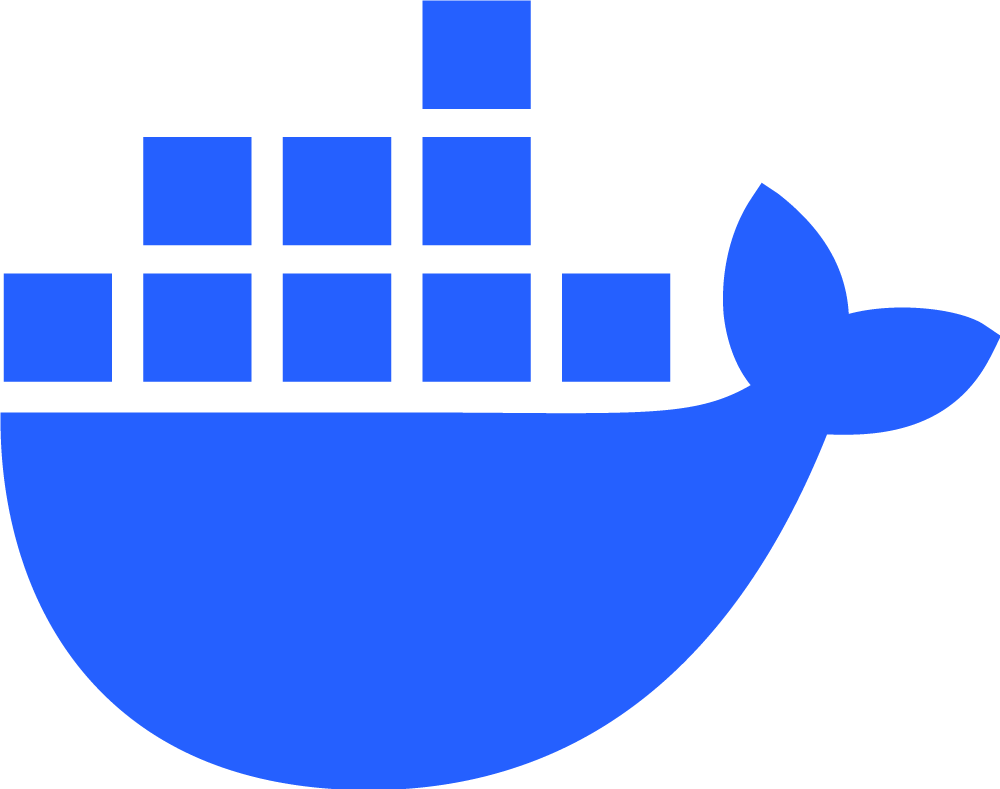
\includegraphics[height=1.4cm, keepaspectratio]{figures/docker.png}
\caption{Docker\cite{docker_logo}}
\label{fig:docker_logo_atb}
\end{figure}
\FloatBarrier
\end{itemize}

\textbf{4. Machine Learning}
\begin{itemize}
    \item \textbf{Scikit-learn}: preprocessing pipelines, metrics, \textbf{Random Forest},
    \textbf{Extra Trees}, \textbf{Logistic Regression}, and model selection utilities
    \cite{breiman2001, hastie2009}.
    \item \textbf{XGBoost}: primary customer risk classifier \cite{chen2016}.
    \item \textbf{MLflow}: experiment tracking, model registry, and production model traceability
    \cite{zaharia2018}.
\end{itemize}

\begin{figure}[H]
\centering
\includegraphics[height=1.5cm, keepaspectratio]{figures/mlflow.png}
\caption{MLflow tool logo\cite{mlflow_logo}}
\label{fig:ml_logos_atb}
\end{figure}
\FloatBarrier

\subsection{Technological Choices: Frontend, Visualisation and Data Analysis}
\begin{itemize}
    \item \textbf{Streamlit}: main operational dashboard framework, selected for rapid
    Python-based BI and ML integration \cite{bhatt2021}.
\begin{figure}[H]
\centering

\includegraphics[height=1.4cm, keepaspectratio]{figures/streamlit.png}
\caption{Streamlit\cite{streamlit_logo}}
\label{fig:streamlit_logo_atb}
\end{figure}
\FloatBarrier

    \item \textbf{Jupyter Notebooks}: ML model development, exploratory data analysis,
    feature engineering, and model selection reporting.
\begin{figure}[H]
\centering

\includegraphics[height=1.4cm, keepaspectratio]{figures/jupyter.png}
\caption{Jupyter Notebooks\cite{jupyter_logo}}
\label{fig:jupyter_logo_atb}
\end{figure}
\FloatBarrier

    \item \textbf{Google Gemini (gemini-2.0-flash)}: generative AI API used to explain dashboard
    charts in plain English for banking business users \cite{gemini2024}.
\end{itemize}



\begin{figure}[H]
\centering

\includegraphics[height=1.4cm, keepaspectratio]{figures/gemini.png}
\caption{Google Gemini\cite{gemini_logo}}
\label{fig:gemini_logo_atb}
\end{figure}
\FloatBarrier

%================================================
\section{Conclusion}
%================================================

This chapter established the theoretical, architectural, and functional foundations of the
ATB BI project. The state-of-the-art review covered Business Intelligence in banking
\cite{chaudhuri2011, eckerson2010}, multidimensional modelling and warehouse design approaches
(Kimball, Inmon, and hybrid) \cite{kimball2013, inmon2005}, machine learning paradigms and
evaluation metrics \cite{mitchell1997, lessmann2015}, the three-pillar global risk score
(Equation~\ref{eq:global_risk_score}) with scientific justification \cite{fatf2012, bcbs2011},
MLOps with MLflow \cite{zaharia2018, sculley2015}, generative AI for dashboard explanation
\cite{gemini2024}, and the comparative positioning of reporting frameworks.

The project is situated at the intersection of three mature domains: BI, data warehousing,
and machine learning. It starts from seven raw banking CSV files, loads data into SQL Server,
transforms it with dbt across three layers, builds a constellation warehouse with 8 dimensions
and 2 fact tables (281,960 total rows, 0 null foreign keys), computes customer risk scores
through the weighted three-pillar formula, trains and compares four supervised ML models (XGBoost
selected with F1 = 95.5\%, Random Forest benchmark with F1 = 89.5\%), tracks experiments with
MLflow, and exposes outputs through Streamlit dashboards and Jupyter Notebooks.

The requirements specification identified 7 actor types, 6 functional modules, 7 non-functional
constraints, 11 user stories across 3 sprints and 3 releases, and the three-tier software
architecture governing the implementation. The next chapter presents the detailed design and
implementation of the ATB data pipeline, from ingestion and warehouse construction to machine
learning and reporting deployment.

%================================================
% CHAPTER 1: RELEASE 1 - SOFTWARE FOUNDATIONS AND ORCHESTRATION ENGINE
%================================================

\chapter{Release 1: Software Foundations and Orchestration Engine Deployment}
%================================================

\section{Introduction}
This chapter details the realisation of Release 1, which constitutes the fundamental foundation and engineering core of the ATB BI platform dedicated to customer risk management. The development of this version was divided into two sprints (Sprint 1 and Sprint 2) driven according to the Scrum methodology. The main objective of this first iteration is twofold: automate the creation of a secure environment (authentication, RBAC) and deploy the central orchestration engine (Apache Airflow), the true autonomous conductor of the system, capable of piloting the entire infrastructure without human intervention.

%================================================
\section{Sprint 1: Setting up the Environment, Security and Profiles}
%================================================

\subsection{Sprint 1 Presentation}
This first development increment establishes the security and environmental foundations of the banking platform. The major technical challenge lies in the total automation of the deployment (via Runbooks) and in the strict segregation of access between the different hierarchical levels of the bank (Central General Management, Risk Manager, Branch Manager).

The objective is to provide a robust installation script (\texttt{MASTER\_DEPLOYMENT\_RUNBOOK}) which configures the Python virtual environment, manages dependencies and initialises the security database. The front-end software interface is developed under the \textbf{Streamlit} framework, with asynchronous management of user sessions (\textit{st.session\_state}) to guarantee the security of future accesses.

%------------------------------------------------
\subsection{Sprint Backlog}

Table \ref{tab:sprint1_backlog} details the functional requirements selected for this first sprint, formalised as User Stories.

\begin{table}[H]
\centering
\caption{Sprint Backlog of Sprint 1}
\label{tab:sprint1_backlog}
\renewcommand{\arraystretch}{1.6}
\resizebox{\textwidth}{!}{
\begin{tabular}{|c|c|p{3cm}|p{6cm}|p{4.5cm}|}
\hline
\rowcolor{blue!15}
\textbf{ID} & \textbf{Priority} & \textbf{As a...} & \textbf{I want to...} & \textbf{So that...} \\
\hline
\textbf{US 1} & High & User (All Roles) & authenticate via a secure login interface & I can access my role-restricted analytical workspace safely. \\
\hline
\textbf{US 2} & High & Central General Management & create, modify, or deactivate user accounts in the console & I can control who has access to the platform (e.g. adding new Branch Managers). \\
\hline
\end{tabular}
}
\end{table}

%------------------------------------------------
\subsection{Global Modelling}

\subsubsection{Global Use Case Diagram of Sprint 1}

The use case diagram (Figure \ref{fig:uc_sprint1}) models the initial interactions of the actors with the system. The "Authenticate" use case is a mandatory passage point (\textit{include}) for any access to the application.

\begin{figure}[H]
\centering
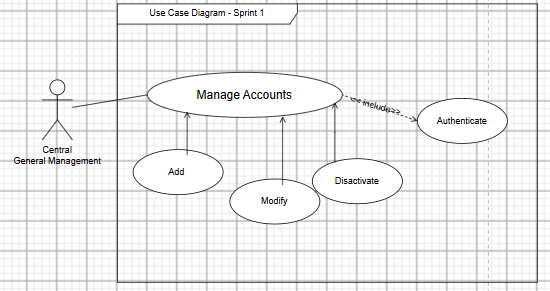
\includegraphics[width=0.9\textwidth]{figures/UseCaseDiagramSprint1.png}
\caption{Global use case diagram of Sprint 1}
\label{fig:uc_sprint1}
\end{figure}

\subsubsection{Class Diagram of Sprint 1}

The class diagram (Figure~\ref{fig:class_sprint1}) illustrates the role-based inheritance structure implemented in the security layer. The base \texttt{User} class defines common attributes such as \texttt{id}, \texttt{username}, \texttt{email}, \texttt{password\_hash}, \texttt{role}, and \texttt{status}. Three specialised subclasses inherit from it: \texttt{DGCentrale} (Central General Management) with administrative privileges, \texttt{RiskManager} for risk oversight, and \texttt{BranchManager} for agency-level access. The \texttt{AuthManager} class handles authentication logic and interacts with the \texttt{User} class to validate credentials and manage sessions.

\begin{figure}[H]
\centering
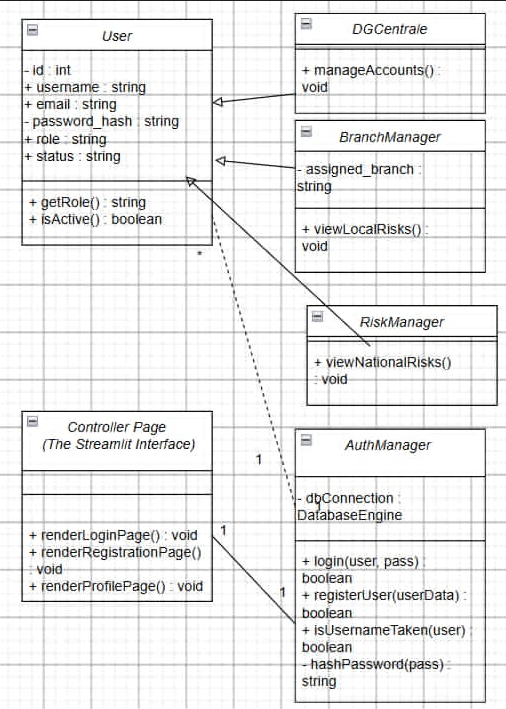
\includegraphics[width=0.82\textwidth]{figures/ClassDiagramSprint1.png}
\caption{Class diagram of Sprint 1 with Role Inheritance}
\label{fig:class_sprint1}
\end{figure}
The diagram makes explicit that authentication and session rights are centralised in
\texttt{AuthManager}, while business roles specialise a shared \texttt{User} base --- the
foundation of the RBAC model used throughout the dashboard.

%------------------------------------------------
\subsection{Use Case Refinement}

To validate compliance with the software architecture, the two main use cases of Sprint 1 are described in detail below.

\paragraph{Use Case Analysis: ``Authenticate''}

\begin{table}[H]
\centering
\caption{Textual description: Authenticate}
\label{tab:uc_auth}
\renewcommand{\arraystretch}{1.2}
\resizebox{\textwidth}{!}{
\begin{tabular}{|p{4cm}|p{11cm}|}
\hline
\rowcolor{blue!15}
\textbf{Use Case} & \textbf{Authenticate} \\
\hline
\textbf{Objective} & Secure dashboard access by verifying credentials against the relational database and establishing the session perimeter. \\
\hline
\textbf{Actor} & Central General Management, Branch Manager, Risk Manager \\
\hline
\textbf{Precondition} & The user possesses an active record in the database schema \texttt{PFE\_AUTH}. \\
\hline
\textbf{Postcondition} & The session variable \texttt{st.session\_state["auth\_user"]} is populated. \\
\hline
\textbf{Nominal Scenario} & 
1. The user connects to the Streamlit gateway page. \newline
2. The user enters their Username and Password. \newline
3. \texttt{AuthManager} hashes the password: $\text{SHA-256}(\text{"ATB\_BI\_2026:"} + \text{password})$. \newline
4. The system queries SQL Server table \texttt{PFE\_AUTH.dashboard\_users} using a parameterised statement. \newline
5. If the record matches, the user's display name, role key, and page rights are loaded. \newline
6. The user is redirected to their default home page dashboard. \\
\hline
\textbf{Alternative Scenario} & 
--- \textbf{Inactive User account} (\texttt{is\_active = 0}): Display *"Access denied. Account is inactive."* \newline
--- \textbf{Invalid Credentials}: Display *"Incorrect username or password."* \\
\hline
\end{tabular}
}
\end{table}

\begin{figure}[H]
\centering
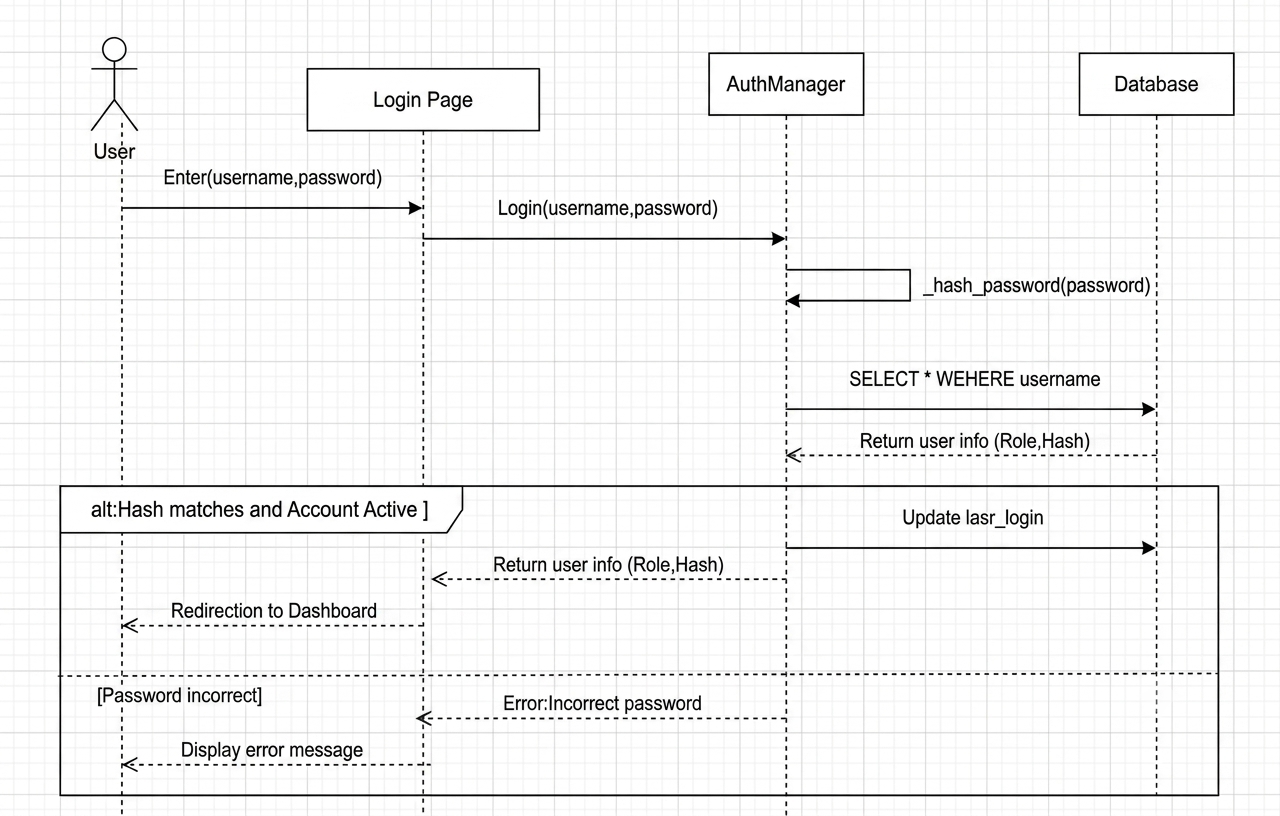
\includegraphics[width=0.85\textwidth,height=0.48\textheight,keepaspectratio]{figures/SequanceDiagramSprint1.png}
\caption{Sequence diagram: User Login}
\label{fig:seq_auth}
\end{figure}
The sequence shows credential capture on the login page, password hashing in
\texttt{AuthManager}, database lookup, and the success/failure alternatives that either
redirect to the dashboard or display an error.

\paragraph{Use Case Analysis: ``Manage Accounts''}

\begin{table}[H]
\centering
\caption{Textual description: Manage Accounts}
\label{tab:uc_manage_accounts}
\renewcommand{\arraystretch}{1.2}
\resizebox{\textwidth}{!}{
\begin{tabular}{|p{4cm}|p{11cm}|}
\hline
\rowcolor{blue!15}
\textbf{Use Case} & \textbf{Manage Accounts (Add/Modify/Deactivate)} \\
\hline
\textbf{Objective} & Allow the administrator (Central GM) to manage the cohort of platform users. \\
\hline
\textbf{Actor} & Central General Management \\
\hline
\textbf{Precondition} & The logged-in user possesses the role code \texttt{DG\_CENTRAL}. \\
\hline
\textbf{Postcondition} & The table \texttt{PFE\_AUTH.dashboard\_users} reflects the transaction. \\
\hline
\textbf{Nominal Scenario} & 
1. The administrator navigates to the "User Administration Console" page. \newline
2. They fill in the registration details (Username, Email, Display Name, Role, and optional Branch/DAO area). \newline
3. \texttt{AccountManager} checks for username uniqueness. \newline
4. \texttt{AccountManager} inserts the new record into the database. \newline
5. The administration table is dynamically refreshed. \\
\hline
\textbf{Alternative Scenario} & 
--- \textbf{Duplicate Detected}: Error message *"This username is already taken."* \\
\hline
\end{tabular}
}
\end{table}

\begin{figure}[H]
\centering
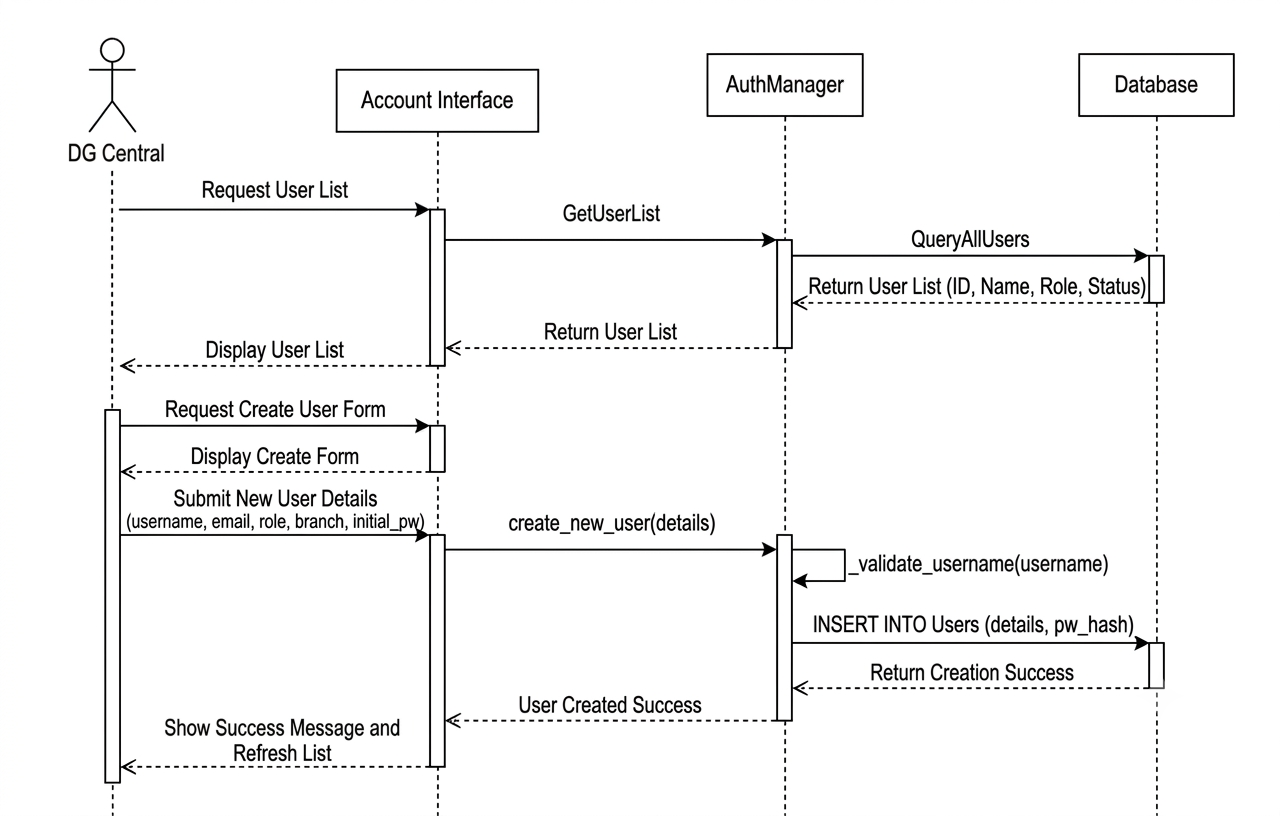
\includegraphics[width=0.85\textwidth,height=0.48\textheight,keepaspectratio]{figures/Sequance2DiagramSprint1.png}
\caption{Sequence diagram: Add New User via mangement}
\label{fig:seq_manage_accounts}
\end{figure}
This second sequence covers account creation and update by Central GM: uniqueness checks,
persistence in \texttt{PFE\_AUTH.dashboard\_users}, and refresh of the administration table.

%------------------------------------------------
\subsection{Sprint 1 Realisation}

The technical implementation of this sprint has been materialised through two distinct layers: database setup and application-level routing. The database schema PFE\_AUTH is configured in SQL Server using the setup\_auth.sql script. This script establishes the relational structures for system roles and the dashboard pages.

The application connects to SQL Server utilizing the SQLAlchemy engine configured with the pyodbc dialect using connection pooling parameters. Password verification is performed securely using Python's hashlib library by encoding the password payload combined with the custom cryptographic salt before running SHA-256. 

User session variables are managed securely via Streamlit's Session state. For Branch Managers, row-level data access is locked dynamically using the Branch filters helper, which appends geographic scopes directly to downstream analytical SQL queries, maintaining absolute security isolation.

\begin{figure}[H]
\centering
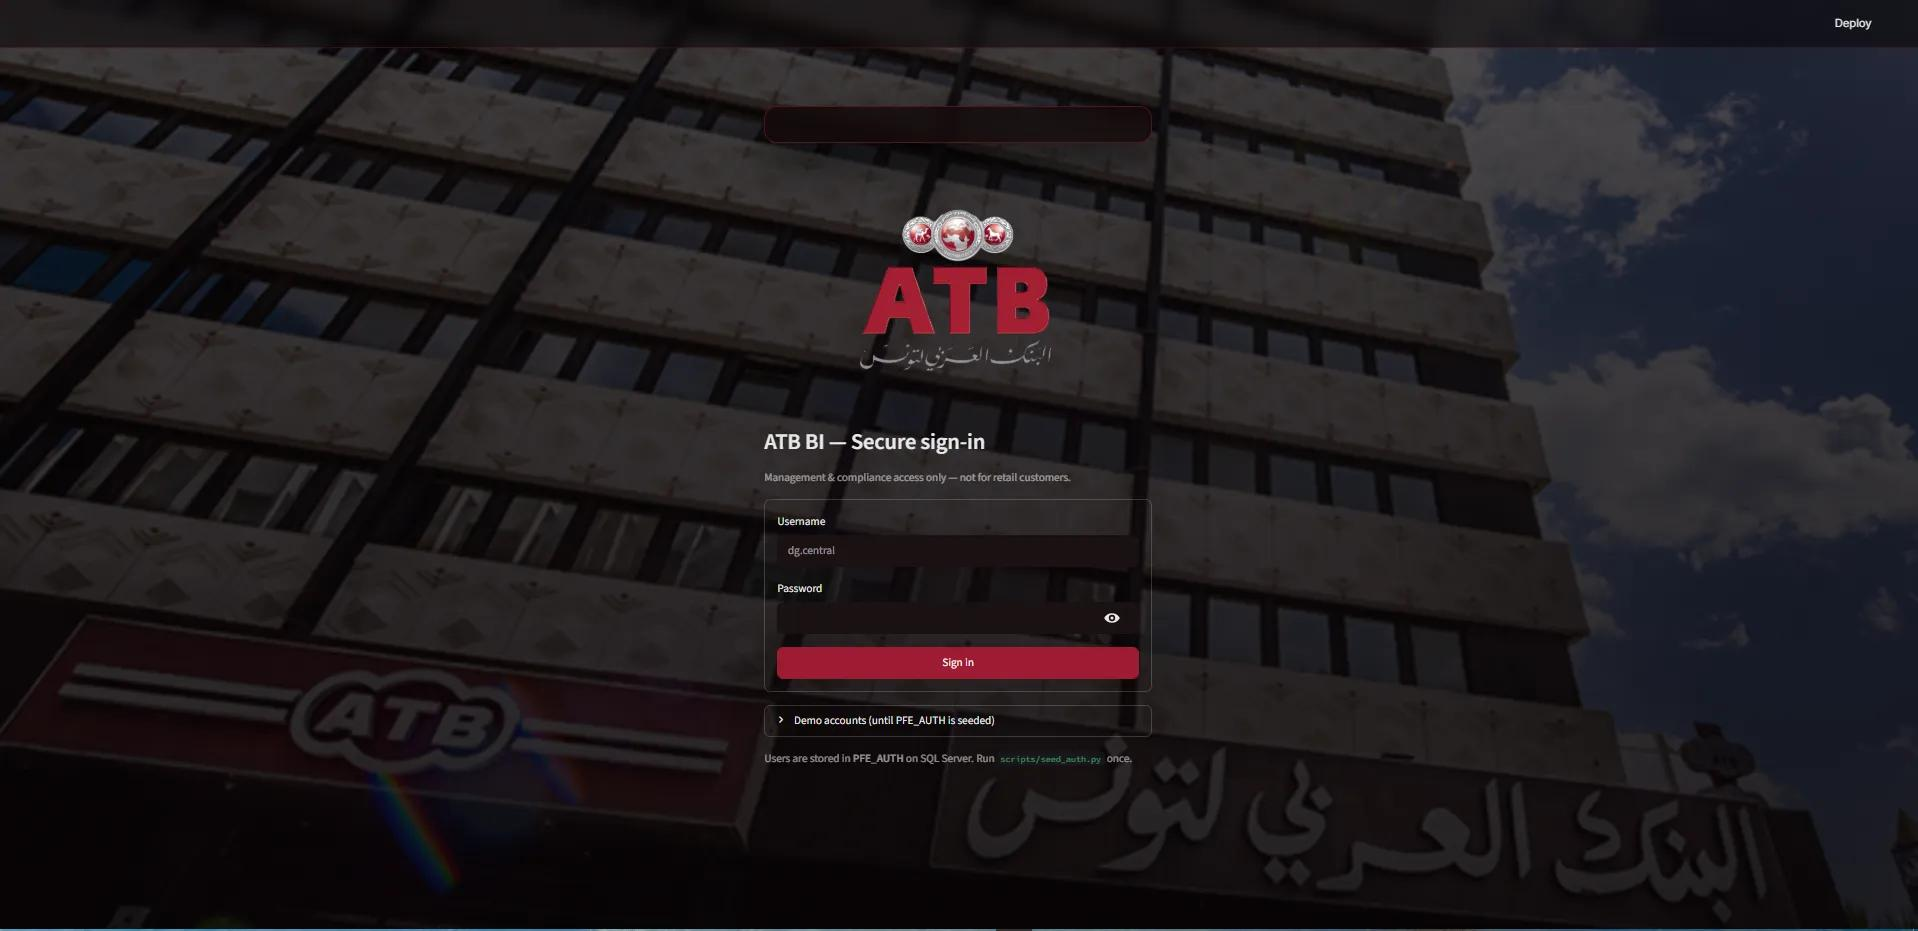
\includegraphics[width=0.85\textwidth]{figures/login_streamlit.png}
\caption{Interface: Secure authentication page (Streamlit)}
\label{fig:ui_login}
\end{figure}
The login gateway is the mandatory entry point for every role: credentials are verified
against \texttt{PFE\_AUTH} before any analytical page is exposed.

\begin{figure}[H]
\centering
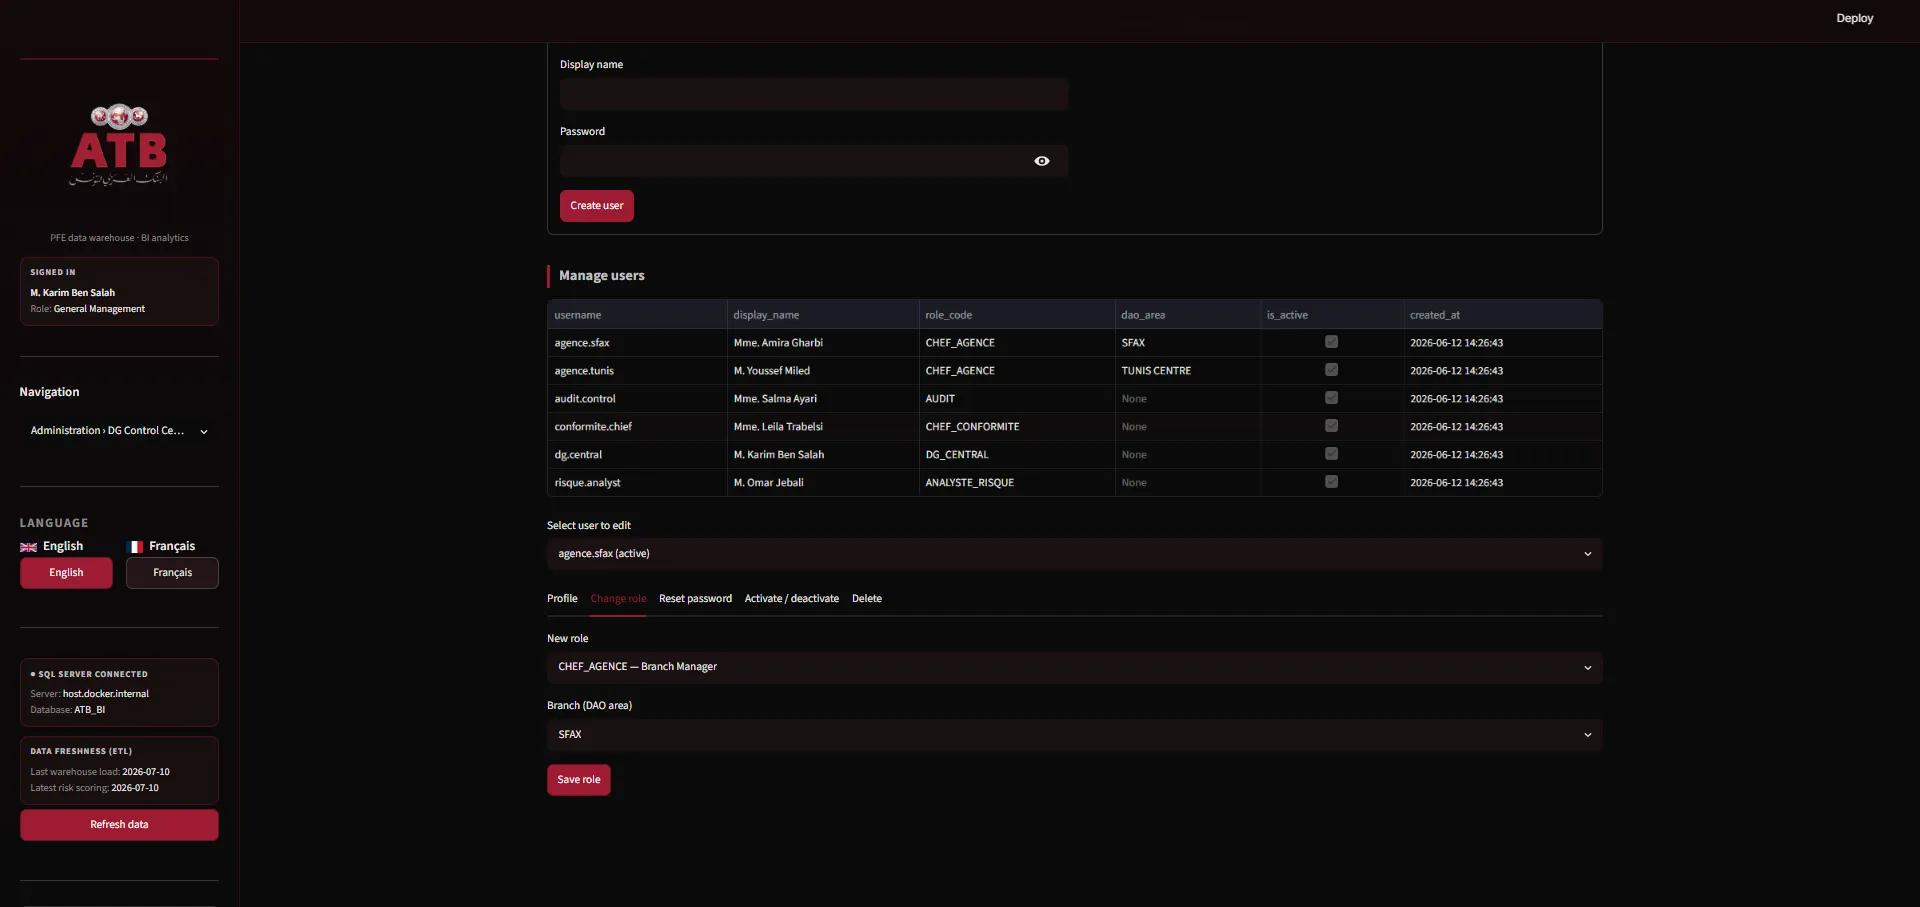
\includegraphics[width=0.85\textwidth]{figures/admin_panel.png}
\caption{Interface: Administration panel for Central GM}
\label{fig:ui_admin}
\end{figure}
Central General Management can create, update and deactivate dashboard users from this
console, enforcing US~02 without direct SQL access.

\begin{figure}[H]
\centering
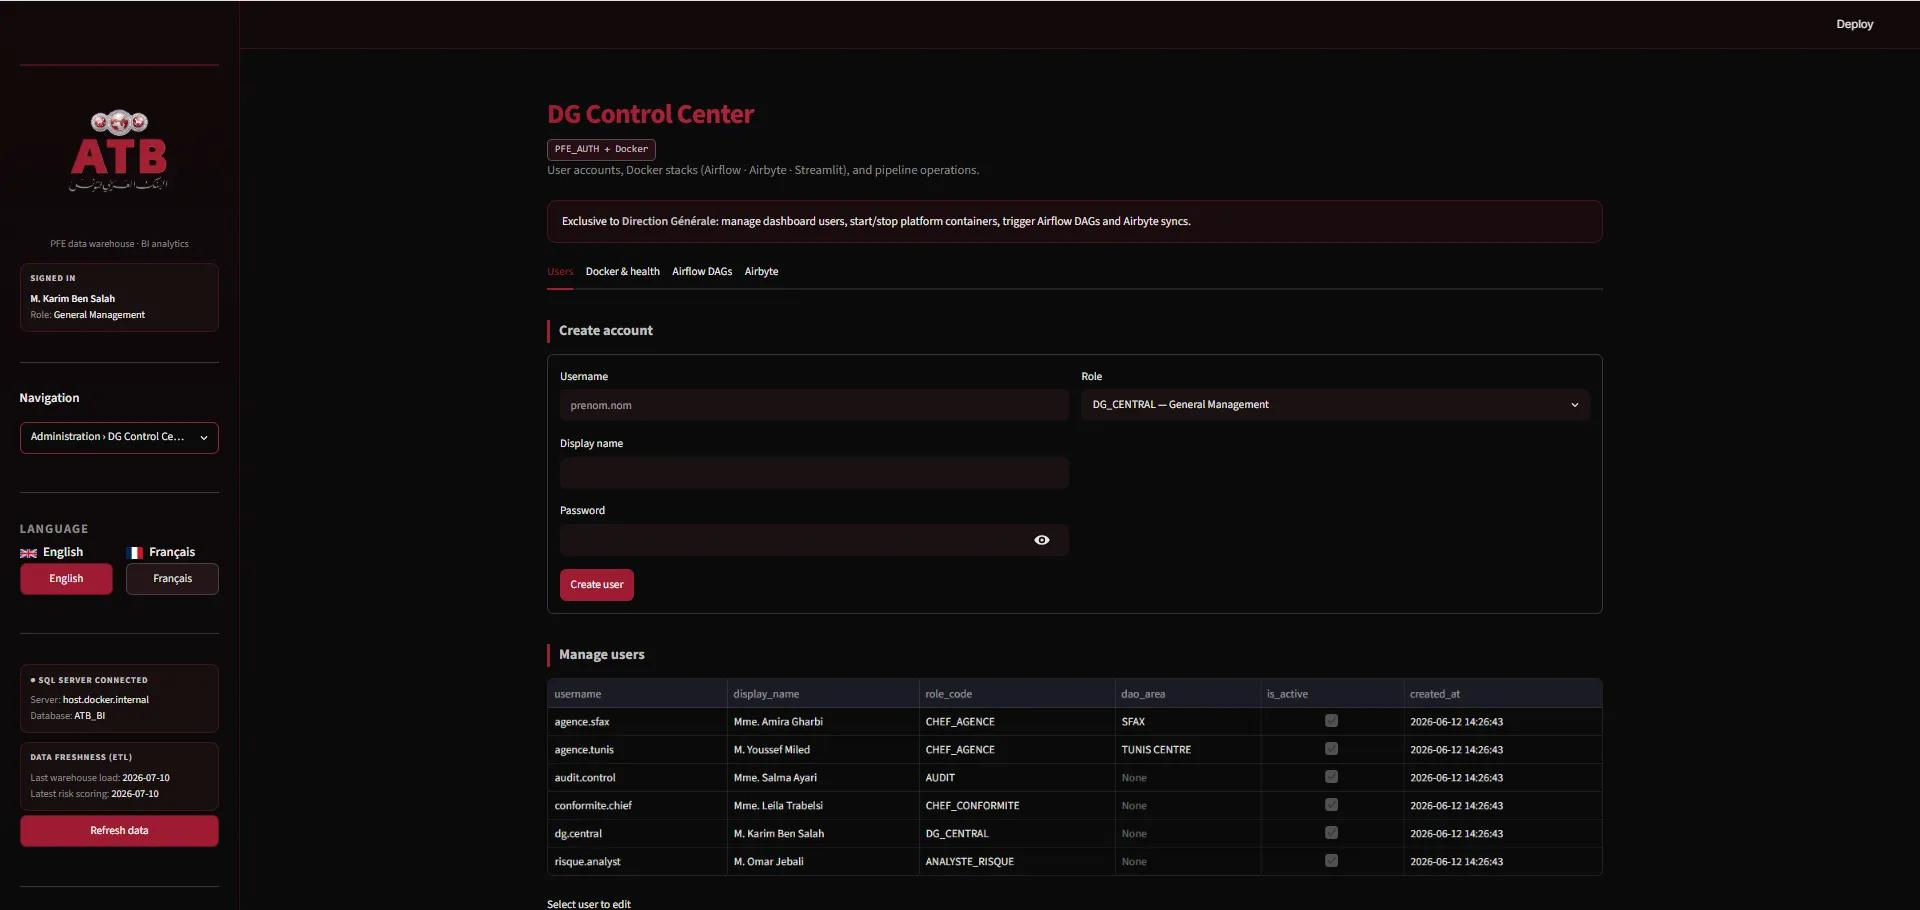
\includegraphics[width=0.85\textwidth]{figures/admin_panel2.png}
\caption{Interface: Detailed administration panel for Central GM}
\label{fig:ui_admin_detail}
\end{figure}
The detailed view lists active accounts with role and branch scope, confirming that
session rights and DAO filters remain consistent after each administration change.
%================================================
\section{Sprint 2: Deploying the Orchestration Engine}
%================================================

\subsection{Sprint 2 Overview}

With the software foundation secured and authenticated during Sprint 1, this second
sprint confronts the deeper challenge: making the platform \textit{think and act on
its own}. A data architecture is only as valuable as its ability to deliver fresh,
reliable information — consistently, automatically, and without depending on a human
to press a button each morning.

Without an orchestration layer, even the most sophisticated data pipeline is little
more than a collection of scripts that someone has to remember to run. In a banking
environment, where decisions are made daily on the basis of financial indicators, that
kind of fragility is simply unacceptable. Data must arrive on time, every time.

This sprint therefore focuses on deploying and configuring \textbf{Apache Airflow}, a
professional-grade workflow orchestration platform widely adopted across the data
engineering industry. Rather than running jobs manually or relying on fragile scheduled
scripts, Airflow allows the engineering team to define the entire data pipeline as a
structured programme — a \textbf{Directed Acyclic Graph (DAG)} — where each step knows
exactly what must happen before it, what it must produce, and what comes after it.

A critical architectural decision was made from the outset: the \textbf{entire
orchestration infrastructure is containerised using Docker}. Rather than installing
Airflow directly on a server — with all the configuration complexity, dependency
conflicts, and environment inconsistency that entails — every component runs inside
its own isolated Docker container, orchestrated together via Docker Compose. This
means the platform can be launched on any machine with a single command, the
environment is perfectly reproducible across development and production, and each
service is isolated from the others yet fully networked. Three dedicated containers
handle the workload: the \textbf{webserver} provides the browser-based monitoring
interface, the \textbf{scheduler} continuously watches the clock and triggers DAGs
at their configured times, and the \textbf{triggerer} manages long-running asynchronous
tasks. A fourth container runs a \textbf{PostgreSQL} database that stores Airflow's
own internal state — run history, task logs, variables, and connections — ensuring
that all operational data survives container restarts.

The pipeline runs automatically every night at 02:00 UTC, so that by the time
the first decision-maker opens the dashboard each morning, all data has already been
silently ingested, cleaned, transformed, validated, and loaded — with zero human
intervention required.

\begin{table}[H]
\centering
\renewcommand{\arraystretch}{1.4}
\caption{Key configuration parameters of the main orchestration pipeline}
\label{tab:dag_config}
\begin{tabular}{|p{4.5cm}|p{9cm}|}
\hline
\rowcolor{blue!15}
\textbf{Parameter} & \textbf{Value / Description} \\
\hline
Pipeline identifier & \texttt{atb\_bi\_warehouse\_etl} \\
\hline
Execution schedule & Every day at 02:00 UTC \\
\hline
Responsible team & Data Engineering \\
\hline
Automatic retries & 2 retries per task in case of failure \\
\hline
Retry delay & 5 minutes between each retry attempt \\
\hline
Failure notification & Automatic alert email sent to the engineering team \\
\hline
Concurrency control & Only one pipeline run active at a time \\
\hline
Historical backfill & Disabled — pipeline only processes current data \\
\hline
Classification tags & Production, ETL, Warehouse \\
\hline
\end{tabular}
\end{table}

%------------------------------------------------
\subsection{Sprint Backlog}

This sprint is built around a single, critical requirement but it is arguably the
most important one in the entire project. Everything built in Release 1 ultimately
serves this goal: a fully autonomous, self-managing data pipeline that guarantees
the daily freshness and integrity of banking data without any manual intervention.

\begin{table}[H]
\centering
\caption{Sprint Backlog of Sprint 2}
\label{tab:sprint2_backlog}
\renewcommand{\arraystretch}{1.6}
\resizebox{\textwidth}{!}{
\begin{tabular}{|c|c|p{3cm}|p{6cm}|p{4.5cm}|}
\hline
\rowcolor{blue!15}
\textbf{ID} & \textbf{Priority} & \textbf{As a\ldots} & \textbf{I want to\ldots} & \textbf{So that\ldots} \\
\hline
\textbf{US 3} & {\textbf{Very High}} &
Central General Management &
have the entire data pipeline orchestrated automatically, so that every stage —
ingestion, transformation, validation — runs without manual involvement &
the bank's data is always fresh, consistent, and trustworthy every single morning,
eliminating the risk of human error or forgotten executions. \\
\hline
\end{tabular}
}
\end{table}

%------------------------------------------------
\subsection{Global Modelling}

\subsubsection{(1) Use Case Diagram}

The use case diagram in Figure~\ref{fig:uc_sprint2} illustrates how the Central General
Management interacts with the orchestration system. The primary action — managing and
monitoring the automated pipeline — is accessible only after authentication, which
remains a mandatory precondition for accessing the Airflow control panel. This ensures
that even the operational monitoring interface is secured within the platform's access
control framework.

\begin{figure}[H]
\centering
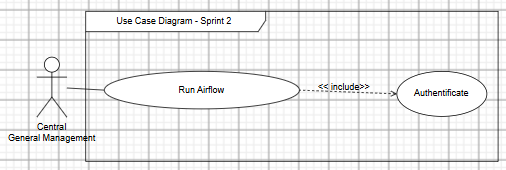
\includegraphics[width=0.9\textwidth]{figures/UseCaseDiagramSprint2.png}
\caption{Global use case diagram of Sprint 2}
\label{fig:uc_sprint2}
\end{figure}

\subsubsection{(2) Class Diagram: Airflow Pipeline Architecture}

Figure~\ref{fig:class_sprint2} represents the object-oriented structure underpinning
the pipeline. The design is organised into four main logical components, each with a
clearly defined responsibility: pipeline configuration and scheduling, task grouping
and dependency management, data quality verification, and runtime environment
configuration. This separation of concerns ensures that each part of the pipeline
can be maintained, tested, and modified independently.

\begin{figure}[H]
\centering
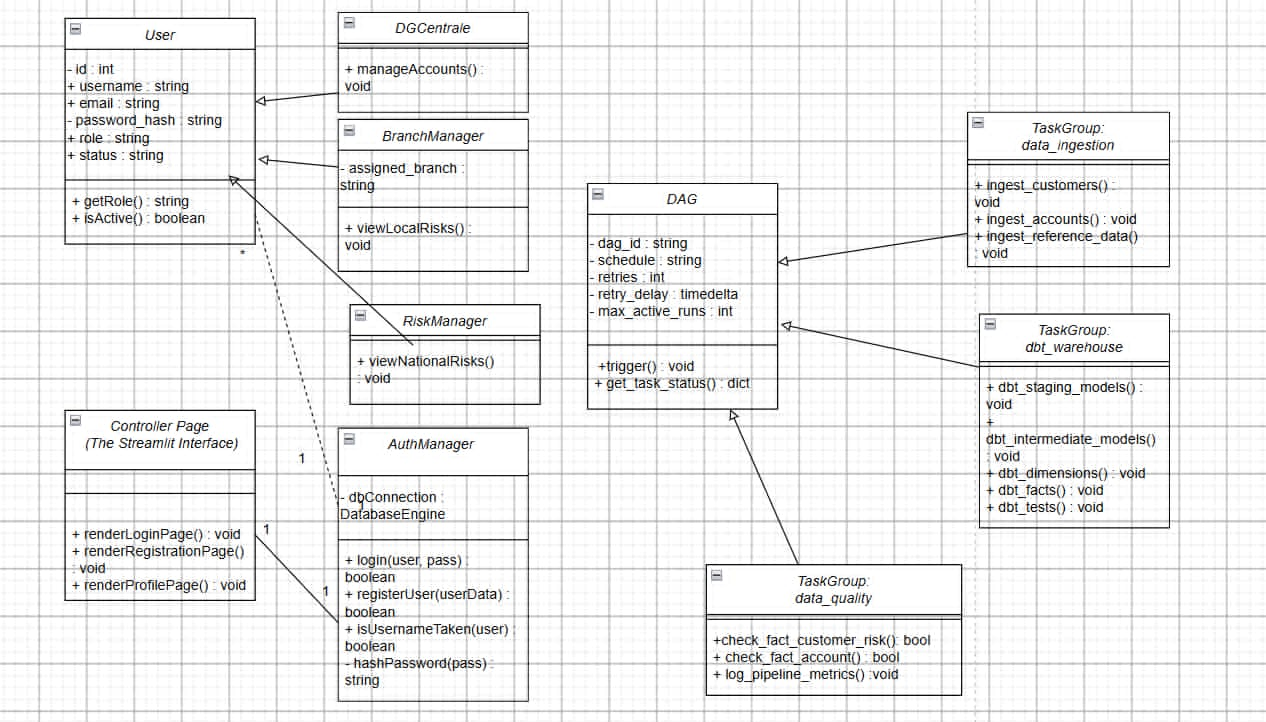
\includegraphics[width=0.9\textwidth]{figures/ClassDiagramSprint2.png}
\caption{Class diagram of Sprint 2 — Airflow DAG architecture}
\label{fig:class_sprint2}
\end{figure}

%------------------------------------------------
\subsection{Use Case Refinement}

\textbf{Use Case Analysis: ``Manage ETL (Airflow Orchestration)''}

\begin{table}[H]
\centering
\small
\caption{Textual description: Manage ETL (Airflow Orchestration)}
\label{tab:uc_airflow}
\renewcommand{\arraystretch}{1.2}
\resizebox{\textwidth}{!}{
\begin{tabular}{|p{3.5cm}|p{12.5cm}|}
\hline
\rowcolor{blue!15}
\textbf{Use Case} & \textbf{Manage ETL (Airflow Orchestration)} \\
\hline
\textbf{Objective} &
Supervise, monitor, and fully automate the banking data pipeline with
enterprise-grade reliability, ensuring consistent daily delivery of clean, validated
data with no manual intervention required. \\
\hline
\textbf{Actor} & Central General Management \\
\hline
\textbf{Precondition} &
The Airflow Docker stack is running and healthy. All required runtime
configuration variables such as the database connection details, the transformation
environment, and the notification endpoints  have been properly set up in Airflow's
configuration store. \\
\hline
\textbf{Postcondition} &
All pipeline tasks complete with a success status. Data quality checks confirm the
absence of any integrity violations across both fact tables. A full execution summary
is recorded and made available for review. \\
\hline
\textbf{Nominal Scenario} &
1. The nightly schedule fires automatically at 02:00 UTC. \newline
2. The pipeline initialises, logging the execution date and preparing the runtime context. \newline
3. \textbf{Data Ingestion:}Three parallel tasks simultaneously load data from
seven source files into the operational data store, maximising throughput. \newline
4. \textbf{Staging Transformation:} Raw ingested data is cleaned, standardised, and
cast into consistent formats, removing any noise introduced by the source systems. \newline
5. \textbf{Intermediate Transformation:}  Business logic is applied: risk pillars are
computed and relationships between entities are established. \newline
6. \textbf{Warehouse Loading:} Dimension tables are built first, followed by the two
central fact tables, respecting referential integrity at every step. \newline
7. \textbf{Schema Testing:}Automated tests verify that all constraints, data types,
and relationships are satisfied. \newline
8. \textbf{Data Quality Checks:}  Two independent verification tasks run in parallel,
probing both fact tables for NULL foreign keys and confirming that row counts meet
the expected minimum thresholds. \newline
9. \textbf{Metrics Logging:} Row counts and key indicators are aggregated into a
comprehensive execution summary, accessible to the engineering team. \newline
10. \textbf{Pipeline Completion:} The pipeline concludes successfully and optionally
triggers the downstream machine learning pipeline for further processing. \\
\hline
\textbf{Alternative Scenario} &
--- \textbf{Integrity violation detected}: If any NULL foreign key is found in a fact
table, the pipeline raises an error immediately, halting further execution and
triggering the automatic retry mechanism. \newline
--- \textbf{Insufficient data volume}: If a fact table contains fewer rows than the
defined minimum threshold, the pipeline treats this as a data anomaly, raises a
diagnostic error, and prevents downstream tasks from consuming potentially incomplete
data. \newline
--- \textbf{Transformation failure}: If a transformation step fails at any point, the
pipeline propagates the failure upward, blocks all dependent tasks, and dispatches an
automatic alert to the engineering team. \\
\hline
\end{tabular}
}
\end{table}

%------------------------------------------------
\subsection{Activity Diagram: Automated Pipeline Execution Flow}

The activity diagram in Figure~\ref{fig:activity_sprint2} models the control flow and
parallel execution branches of the \texttt{atb\_bi\_warehouse\_etl} pipeline. It details the
sequential stages --- from initial cron scheduling, parallel source ingestion into
\texttt{PFE\_ODS}, three-tier dbt transformations, parallel fact quality checks, to the conditional
downstream machine learning trigger.

\begin{figure}[H]
\centering
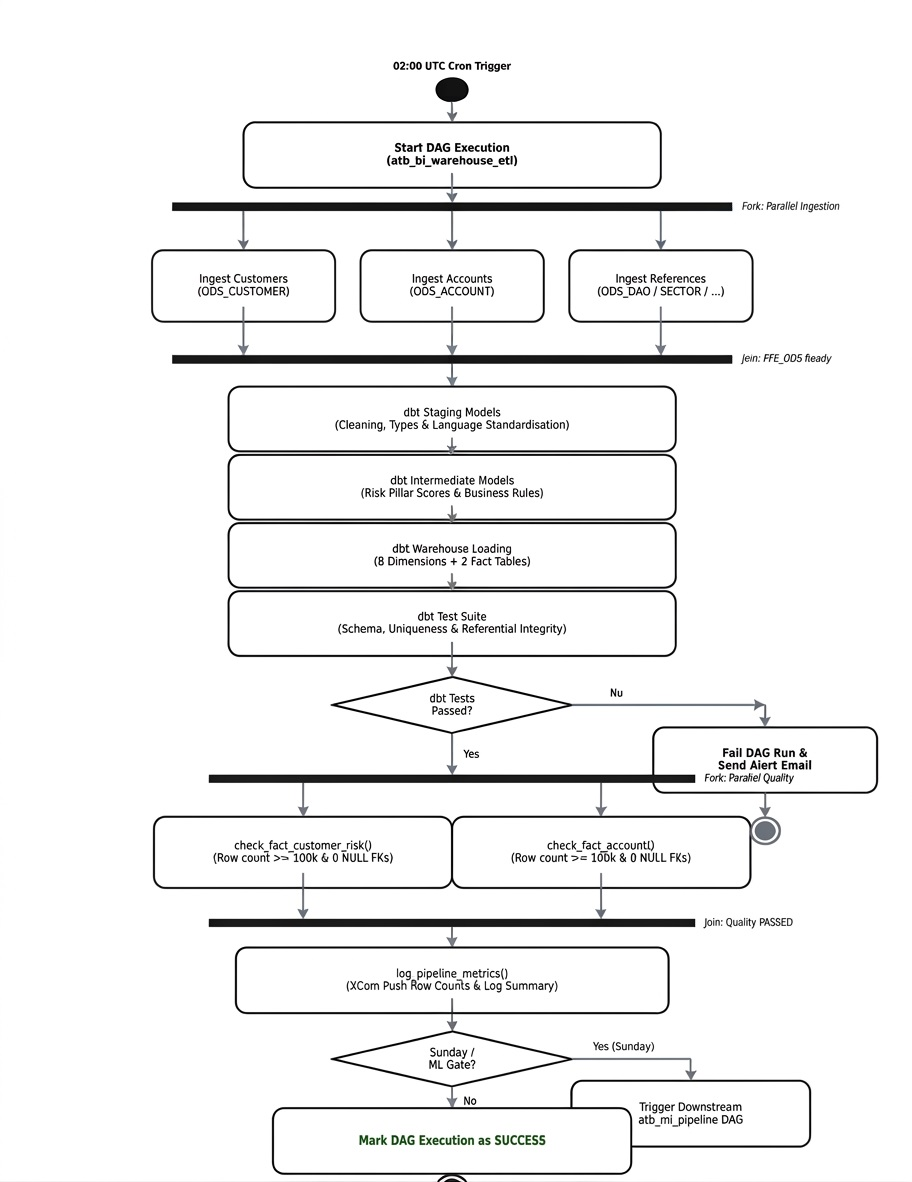
\includegraphics[width=0.7\textwidth]{figures/ActivityDiagramAIRFLOW1.png}
\caption{Activity diagram: end-to-end automated pipeline execution flow}
\label{fig:activity_sprint2}
\end{figure}

%------------------------------------------------
\subsection{Sprint 2 Realisation}

\subsubsection{Infrastructure: A Fully Containerised Platform and DevOps Work}

Before discussing what the pipeline does, it is important to understand \textit{how} it runs. A key engineering effort of this project was designing a custom containerised platform rather than relying on generic setups. 

The entire Airflow orchestration infrastructure is packaged as a \textbf{custom Docker image} (\texttt{atb-airflow:2.9.1}), defined in a dedicated \texttt{Dockerfile}. This custom image extends the official base distribution with:
\begin{itemize}
    \item Native Microsoft SQL Server ODBC Driver 17 for direct relational connectivity.
    \item \texttt{dbt-sqlserver} and transformation dependencies allowing Airflow tasks to run dbt models directly inside the container.
    \item Embedded Machine Learning execution packages (\texttt{xgboost}, \texttt{scikit-learn}, \texttt{mlflow}) to support automated retraining DAGs.
\end{itemize}

% --- SCREENSHOT: Add screenshot of 2_orchestration/Dockerfile here
\begin{figure}[H]
\centering
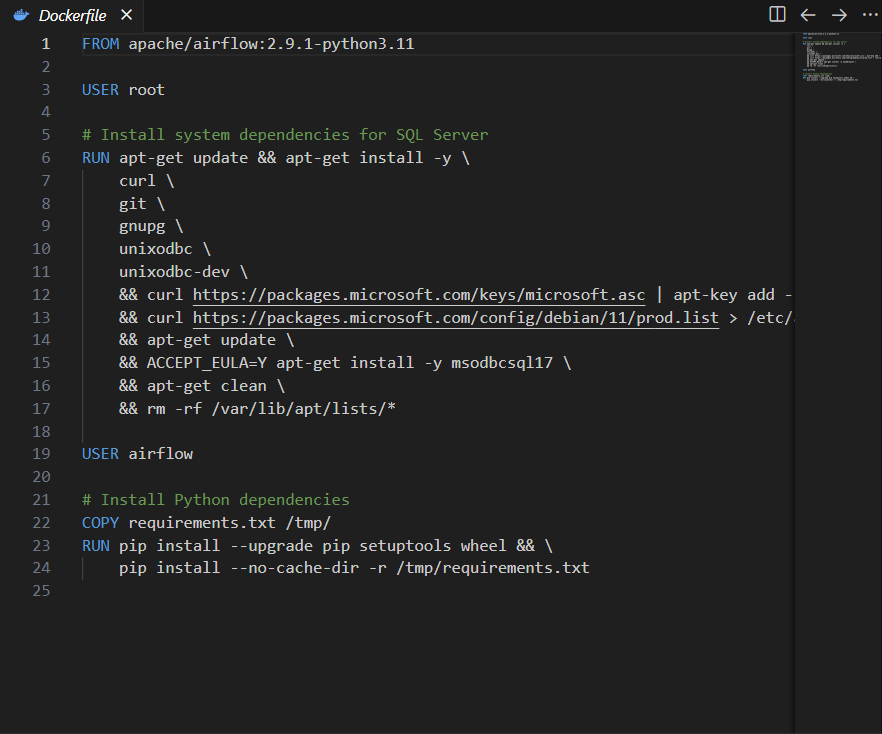
\includegraphics[width=0.88\textwidth]{figures/airflow_dockerfile_yaml.png}
\caption{Custom Dockerfile configuration for the ATB Airflow orchestration container}
\label{fig:airflow-dockerfile-code}
\end{figure}
\noindent Custom Dockerfile specification for the Airflow engine container.

The service architecture is defined in a custom \textbf{\texttt{docker-compose.yml}} specification that orchestrates four coordinated containers:

\begin{table}[H]
\centering
\small
\renewcommand{\arraystretch}{1.4}
\caption{Docker containers composing the Airflow orchestration stack}
\label{tab:docker_containers}
\begin{tabular}{|p{3.5cm}|p{10cm}|}
\hline
\rowcolor{blue!15}
\textbf{Container} & \textbf{Role} \\
\hline
\textbf{Airflow Webserver} &
Serves the browser-based monitoring interface on port 8080. This is where the
engineering team views DAG run histories, task logs, and pipeline status. \\
\hline
\textbf{Airflow Scheduler} &
The engine that watches the clock, evaluates which DAGs are due to run, and
dispatches tasks to available workers. It runs continuously in the background. \\
\hline
\textbf{Airflow Triggerer} &
Handles deferred tasks those that wait for an external event (such as a downstream
DAG completing) without occupying a worker slot. \\
\hline
\textbf{PostgreSQL Database} &
Stores all of Airflow's internal state: run history, task instance logs, variable
values, connection credentials, and user accounts. \\
\hline
\end{tabular}
\end{table}

% --- SCREENSHOT: Add screenshot of 2_orchestration/docker-compose.yml here
\begin{figure}[H]
\centering
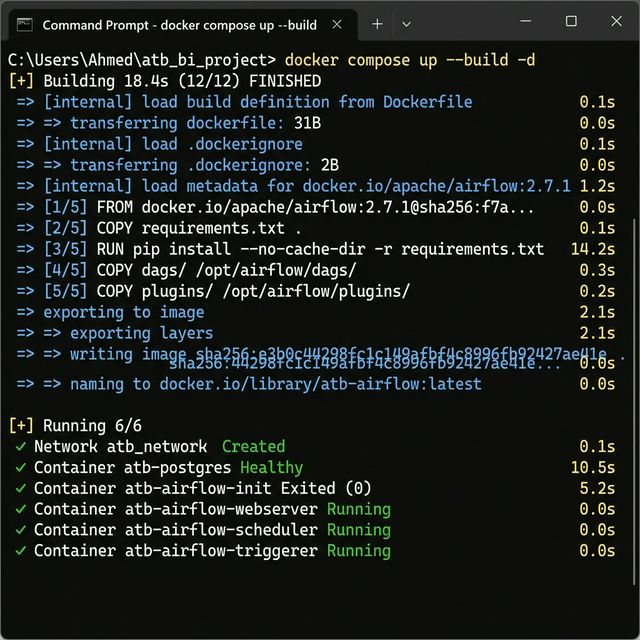
\includegraphics[width=0.88\textwidth]{figures/airflow_docker_compose_yaml.png}
\caption{Custom docker-compose.yml orchestration file for the Airflow stack}
\label{fig:airflow-docker-compose-yaml}
\end{figure}
\noindent % [USER INSTRUCTION]: Place your screenshot of 2_orchestration/docker-compose.yml above (uncomment \includegraphics).

All containers share a dedicated bridge network (\texttt{atb-network}) and connect to host-bound services via \texttt{host.docker.internal:host-gateway}. The transformation models, raw datasets, and ML sources are mounted as volumes into the containers, ensuring instant code updates without container rebuilds.
raw data files are mounted directly into the containers as volumes, so that updates to
the pipeline code take effect without needing to rebuild the image. The platform can
be brought up or torn down entirely in seconds.

\subsubsection{The DAG Ecosystem: Four Pipelines, One Platform}

One of the strengths of the Airflow implementation is that it does not rely on a single
monolithic pipeline. Instead, the engineering team designed a \textbf{family of four
complementary DAGs}, each with a distinct responsibility. Together they form a
layered orchestration ecosystem, where each DAG can operate independently or be
triggered as part of a larger chain.

\paragraph{DAG 1: The Master Pipeline}

This is the backbone of the entire platform and the DAG that runs every single night.
Designed as the comprehensive end-to-end orchestrator, it takes full ownership of the
data lifecycle from ingestion through transformation to machine learning, combining the
responsibilities of warehouse loading and production orchestration into a single,
authoritative pipeline.

The pipeline is built as a sequence of nine tasks organised into three task groups.
It begins by attempting to synchronise data via Airbyte the dedicated ingestion
platform and falls back gracefully if Airbyte is not configured, validating instead
that the operational data store already contains fresh data. A \textbf{parallel
ingestion phase} then loads customer data, account data, and all reference tables
(currencies, sectors, industries, organisational units, and risk targets) simultaneously.
Once ingestion is confirmed, a \textbf{three-layer transformation phase} takes over:
the staging layer cleans and standardises the raw data, the intermediate layer applies
business logic and computes risk indicators, and the warehouse layer first populates
eight dimension tables before building the two central fact tables on top of them.
A structural testing phase runs automatically to verify all constraints and data types,
followed by a \textbf{parallel data quality phase} that probes both fact tables for
NULL foreign keys and confirms row counts above the expected minimum threshold.
A full execution summary is then logged. Uniquely, the pipeline also includes a
\textbf{weekly machine learning gate}: every Sunday, after the warehouse is confirmed
clean, it automatically triggers the XGBoost risk model retraining ensuring the
ML model is refreshed with the most recent banking data every week without any manual
scheduling.

\paragraph{DAG 2: The Standalone Ingestion Pipeline}

This DAG handles data ingestion in isolation. It connects to Airbyte, triggers
synchronisation jobs for each of the seven data sources, waits for them to complete,
and then validates that the resulting data in the operational data store meets minimum
volume expectations. It is designed to be run manually when a fresh data load is
needed outside the normal nightly schedule, or to be called as a component by the
master pipeline when fine-grained control over the ingestion phase is required.

\paragraph{DAG 3: The Standalone Transformation Pipeline}

This DAG covers only the dbt transformation layer. It runs the full sequence of
transformation steps from a connection health check and dependency installation,
through all three model layers (staging, intermediate, warehouse) to a final round
of structural tests and automatic documentation generation. Its purpose is to allow
the engineering team to re-run transformations independently, for example after
correcting a model or deploying new business logic, without needing to re-trigger
the ingestion phase.

\paragraph{DAG 4: The Machine Learning Pipeline}

The final DAG in the ecosystem is dedicated entirely to the machine learning lifecycle.
It can be triggered manually or automatically from the master pipeline on a weekly
basis. It runs the XGBoost customer risk model training script, waits for it to
complete, verifies that the trained model artefact was produced correctly, and then
executes a separate script that writes the model's predictions back into the data
warehouse making them available for display in the Streamlit dashboard. The entire
ML refresh cycle, from training to warehouse update, is therefore fully automated
and requires no human involvement.

\begin{table}[H]
\centering
\small
\renewcommand{\arraystretch}{1.5}
\caption{Summary of DAGs deployed in the Airflow ecosystem}
\label{tab:dag_summary}
\begin{tabular}{|p{4.2cm}|p{2.5cm}|p{7.3cm}|}
\hline
\rowcolor{blue!15}
\textbf{DAG} & \textbf{Schedule} & \textbf{Purpose} \\
\hline
DAG~1 --- Master Pipeline & Daily 02:00 UTC & End-to-end pipeline: Airbyte sync → ingest → transform → test → validate → log → weekly ML trigger \\
\hline
DAG~2 --- Standalone Ingestion & On demand & Airbyte data synchronisation + ODS validation only \\
\hline
DAG~3 --- Standalone Transformation & On demand & Full dbt run across all three model layers + documentation generation \\
\hline
DAG~4 --- Machine Learning Pipeline & Weekly (Sunday) or on demand & XGBoost model retraining + prediction writing to data warehouse \\
\hline
\end{tabular}
\end{table}

\subsubsection{The Main Pipeline in Detail: Nine Steps, One Unbroken Chain}

The nightly warehouse ETL pipeline the DAG that runs automatically every day is
structured into \textbf{nine sequential phases}, logically grouped into three task
groups. This design balances parallelism, where independent tasks can run simultaneously
to save time, with strict ordering, ensuring that no downstream step ever begins before
its upstream dependencies have fully succeeded.

\begin{table}[H]
\centering
\small
\renewcommand{\arraystretch}{1.5}
\caption{Execution phases of the automated data pipeline}
\label{tab:dag_phases}
\begin{tabular}{|c|p{3.5cm}|p{4cm}|p{5cm}|}
\hline
\rowcolor{blue!15}
\textbf{Phase} & \textbf{Task / Group} & \textbf{Mechanism} & \textbf{Output} \\
\hline
1 & Pipeline Start & Shell command & Execution context initialised and logged \\
\hline
2 & \textbf{Data Ingestion} (parallel) & 3 simultaneous tasks & 7 source files loaded into the operational data store \\
\hline
3 & Staging Transformation & Shell command & Raw data cleaned and standardised \\
\hline
4 & Intermediate Transformation & Shell command & Business logic applied; risk pillars computed \\
\hline
5 & \textbf{Warehouse Loading} (sequential) & 2 ordered tasks & 8 dimension tables + 2 fact tables built.\\
\hline
6 & Schema \& Integrity Testing & Shell command & All structural and relational tests pass \\
\hline
7 & \textbf{Data Quality Checks} (parallel) & 2 simultaneous tasks & Zero NULL foreign keys confirmed on both fact tables \\
\hline
8 & Metrics Logging & Python function & Full execution summary produced \\
\hline
9 & Pipeline Completion & Shell command & Success confirmed; ML pipeline optionally triggered \\
\hline
\end{tabular}
\end{table}

The entire dependency structure of the pipeline is expressed in a single, readable
declaration that reflects the architecture at a glance:

\begin{center}
\small
\textit{Start $\rightarrow$ Data Ingestion $\rightarrow$ Staging $\rightarrow$ Intermediate $\rightarrow$ Warehouse $\rightarrow$ Testing $\rightarrow$ Quality Checks $\rightarrow$ Metrics $\rightarrow$ Success}
\end{center}

\subsubsection{Data Quality Framework: Trusting the Numbers}

One of the most critical aspects of a banking data platform is the ability to trust
the numbers it produces. A dashboard showing inaccurate figures is worse than no
dashboard at all  it leads to confident, well-presented errors. To prevent this,
the pipeline embeds a dedicated data quality verification layer that runs automatically
after every transformation cycle.

This layer performs a series of targeted checks against both fact tables, probing for
the specific categories of integrity failure most likely to arise from data ingestion
or transformation issues:

\begin{table}[H]
\centering
\small
\renewcommand{\arraystretch}{1.4}
\caption{Data quality checks embedded in the pipeline}
\label{tab:dq_checks}
\begin{tabular}{|p{4.5cm}|p{4cm}|p{5.2cm}|}
\hline
\rowcolor{blue!15}
\textbf{Check} & \textbf{Scope} & \textbf{Failure Condition} \\
\hline
Customer reference integrity & Both fact tables & Any unresolved customer link raises an error \\
\hline
Organisational unit integrity & Both fact tables & Any unresolved organisational reference raises an error \\
\hline
Currency reference integrity & Account fact table & Any unresolved currency reference raises an error \\
\hline
Industry classification integrity & Customer risk fact table & Any unresolved industry reference raises an error \\
\hline
Risk target reference integrity & Customer risk fact table & Any unresolved risk target reference raises an error \\
\hline
Minimum data volume & Both fact tables & Fewer than 100,000 rows triggers a data anomaly alert \\
\hline
\end{tabular}
\end{table}

When a check passes, it records its result so that the final reporting task can
aggregate all metrics into a single execution summary giving the engineering team
full visibility into every pipeline run, including exactly how many records were
processed across each table.

\subsubsection{Resilience by Design: Configuration and Fault Tolerance}

A production data platform must be both secure and resilient. On the security side,
no sensitive information such as database credentials, server addresses, or
notification endpoints is written directly into the pipeline code. Instead, all
configuration is stored separately in Airflow's secure variable store and injected
at runtime, so that the same pipeline code can run safely across different environments
without modification.

\begin{table}[H]
\centering
\small
\renewcommand{\arraystretch}{1.3}
\caption{Runtime configuration variables injected securely at pipeline execution}
\label{tab:airflow_vars}
\begin{tabular}{|p{4.5cm}|p{9cm}|}
\hline
\rowcolor{blue!15}
\textbf{Configuration Variable} & \textbf{Purpose} \\
\hline
Transformation project path & Tells the pipeline where to find the transformation models \\
\hline
Transformation profile & Identifies which transformation configuration set to use \\
\hline
Execution environment & Specifies whether the pipeline is running in production or development \\
\hline
Database server & Hostname of the target SQL Server instance \\
\hline
Target database & The name of the analytical data warehouse database \\
\hline
Notification endpoint & Webhook URL for real-time failure notifications \\
\hline
\end{tabular}
\end{table}

On the resilience side, every task in the pipeline is configured with a fault-tolerance
policy: if a task fails due to a transient issue a momentary network interruption,
a database timeout, or a brief resource constraint  Airflow will automatically retry
it up to two times, waiting five minutes between each attempt. This window is large
enough for most transient issues to self-resolve, and small enough that the pipeline
still completes well before the business day begins. If all retries are exhausted and
the task remains failed, an automatic alert is dispatched to the engineering team,
ensuring that no failure goes unnoticed.

\subsubsection{Bringing It All Together: The Integrated Monitoring Panel}

One of the most practically powerful features delivered in this sprint is the
\textbf{integration of Airflow monitoring directly into the Streamlit platform}. Rather
than requiring the engineering team or management to open a separate browser tab,
log into Airflow independently, and interpret its technical interface, the Streamlit
dashboard includes a dedicated \textbf{Operations Console} accessible exclusively
to users with the highest administrative privileges.

This console is designed to answer one simple question: \textit{is everything working?}

\begin{figure}[H]
\centering
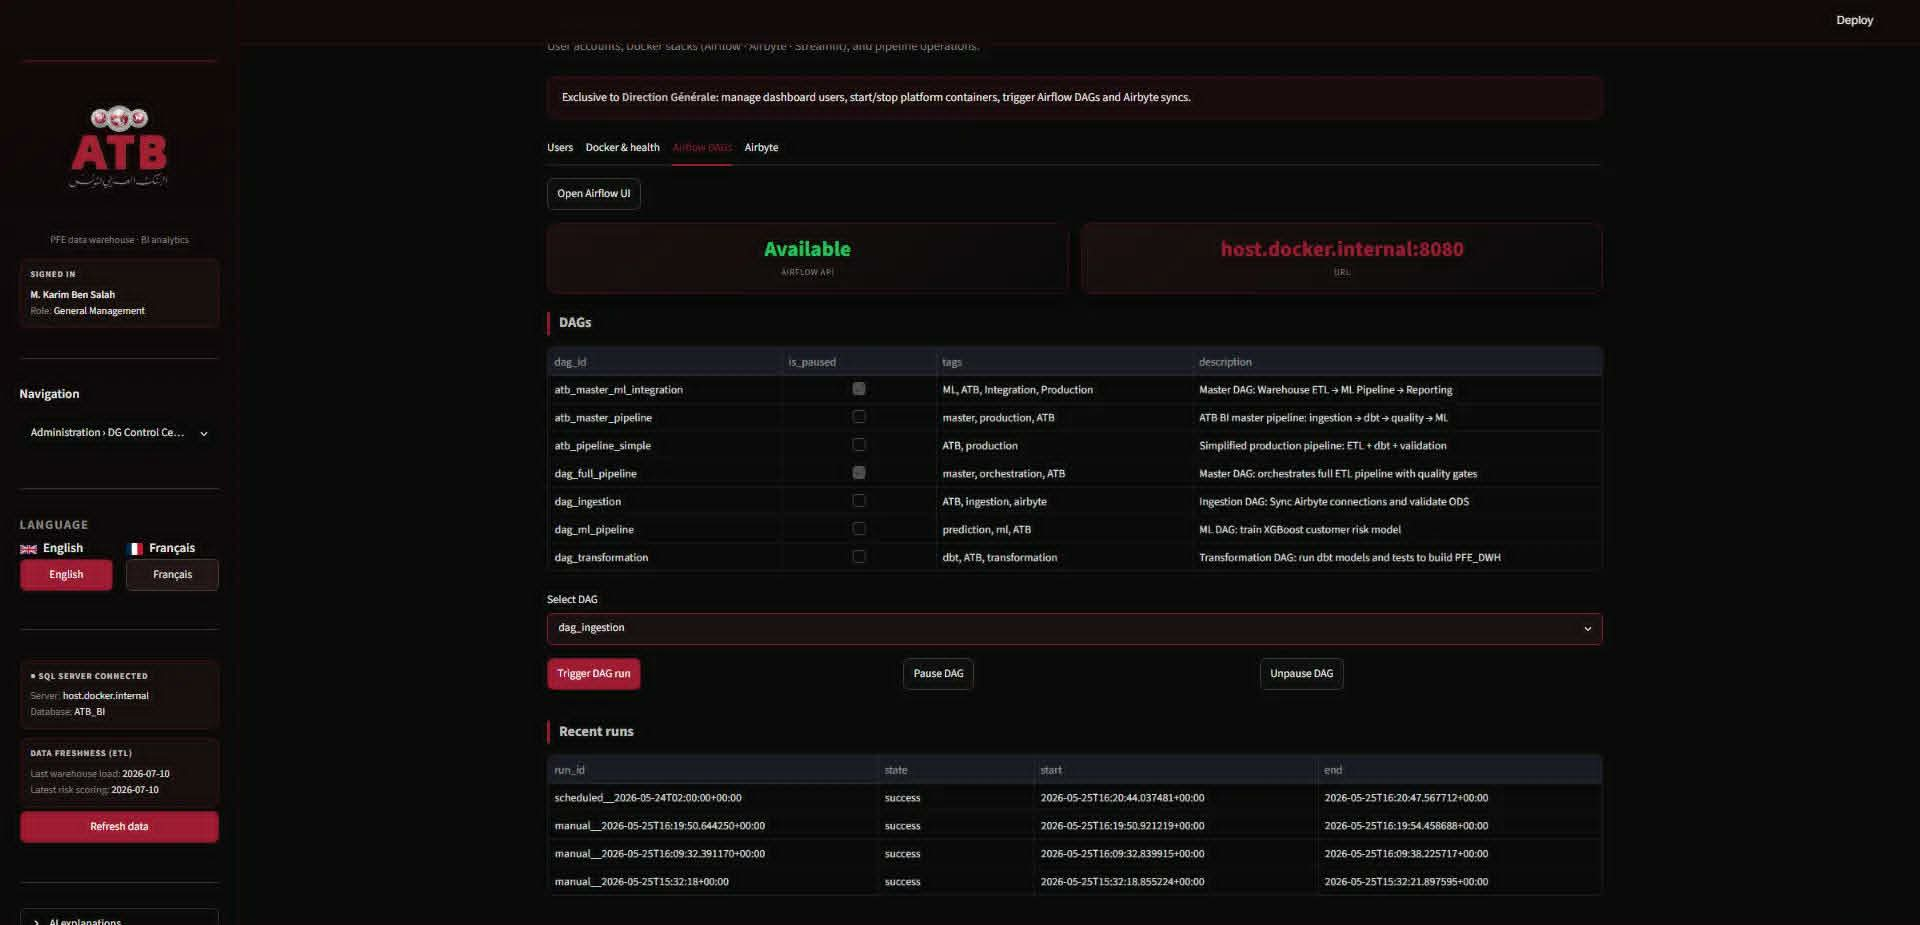
\includegraphics[width=0.9\textwidth]{figures/Streamlit Airflow Panel.png}
\caption{The Airflow monitoring panel embedded in the Streamlit}
\label{fig:streamlit_airflow}
\end{figure}

When a privileged user opens the Airflow tab within the console, the panel
automatically reaches out to the Airflow REST API and retrieves live information
about the current state of the orchestration engine. A set of status indicators at
the top of the panel immediately shows whether Airflow is reachable and healthy
a green signal means the pipeline engine is operational; a red signal triggers an
explanatory warning with guidance on how to restart the stack. Below this, the panel
displays a live table of all DAGs registered in the system, including their
current pause state, their tags, and a short description of their purpose.

\begin{figure}[H]
\centering
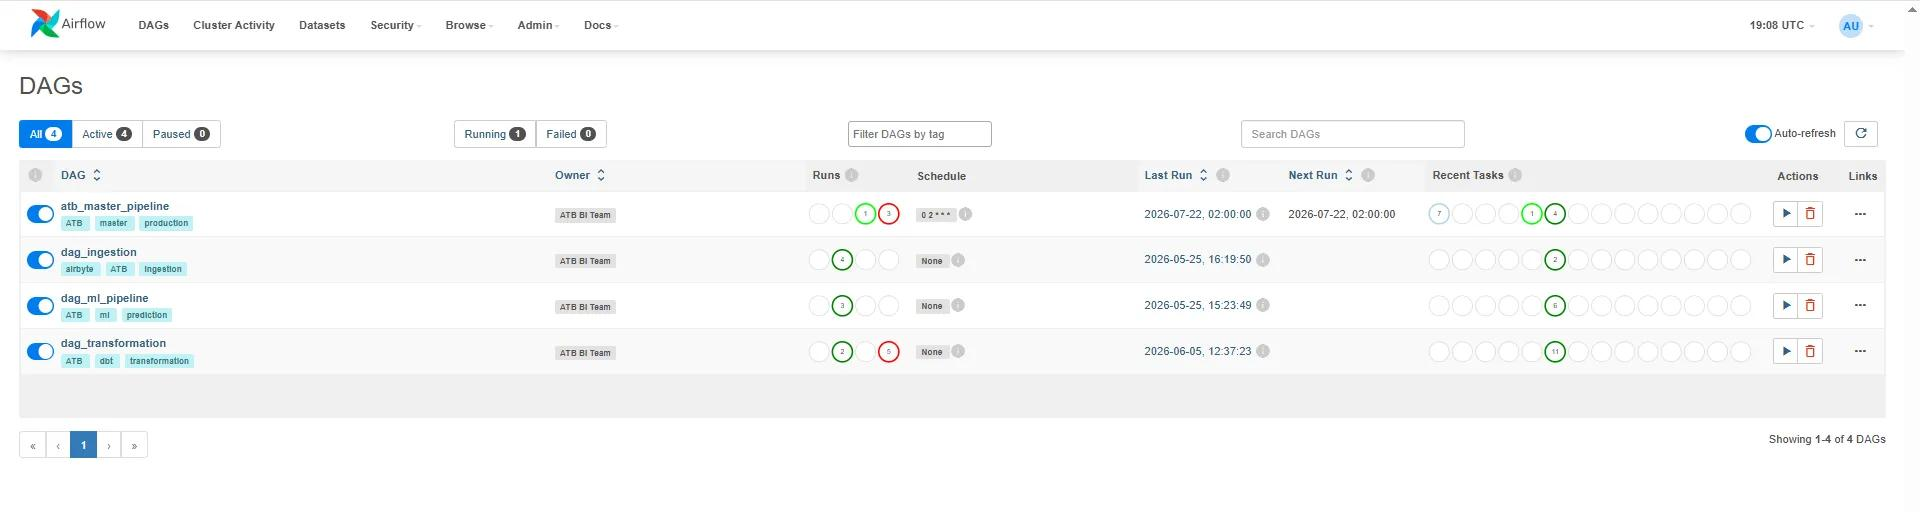
\includegraphics[width=0.9\textwidth]{figures/Airflow Dags List.png}
\caption{Live DAG registry displayed in the AirFlow}
\label{fig:airflow_dags_list}
\end{figure}

The user can select any DAG from the list and see the history of its last ten runs,
including the start and end time of each execution and its final status whether it
completed successfully, failed, or is currently running.

\begin{figure}[H]
\centering
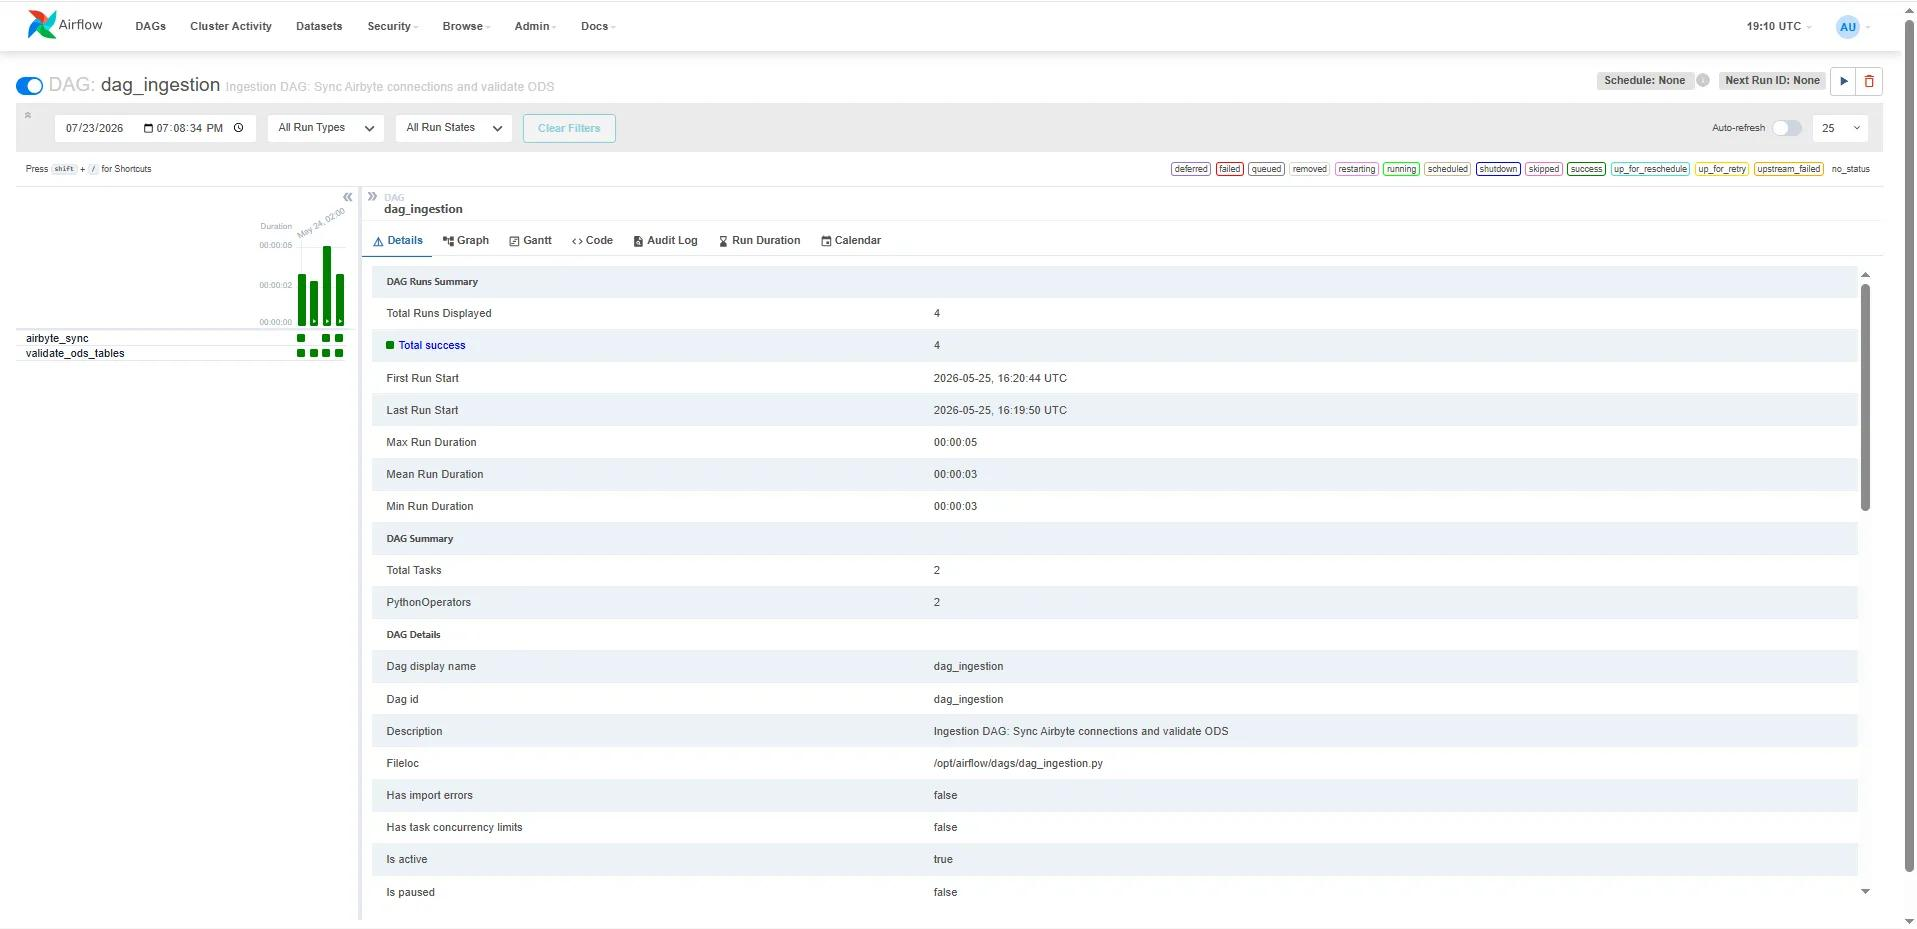
\includegraphics[width=0.9\textwidth]{figures/Dag run satus example.png}
\caption{DAG run history retrieved in real time through the Airflow API}
\label{fig:dag_run_status}
\end{figure}

\begin{figure}[H]
\centering
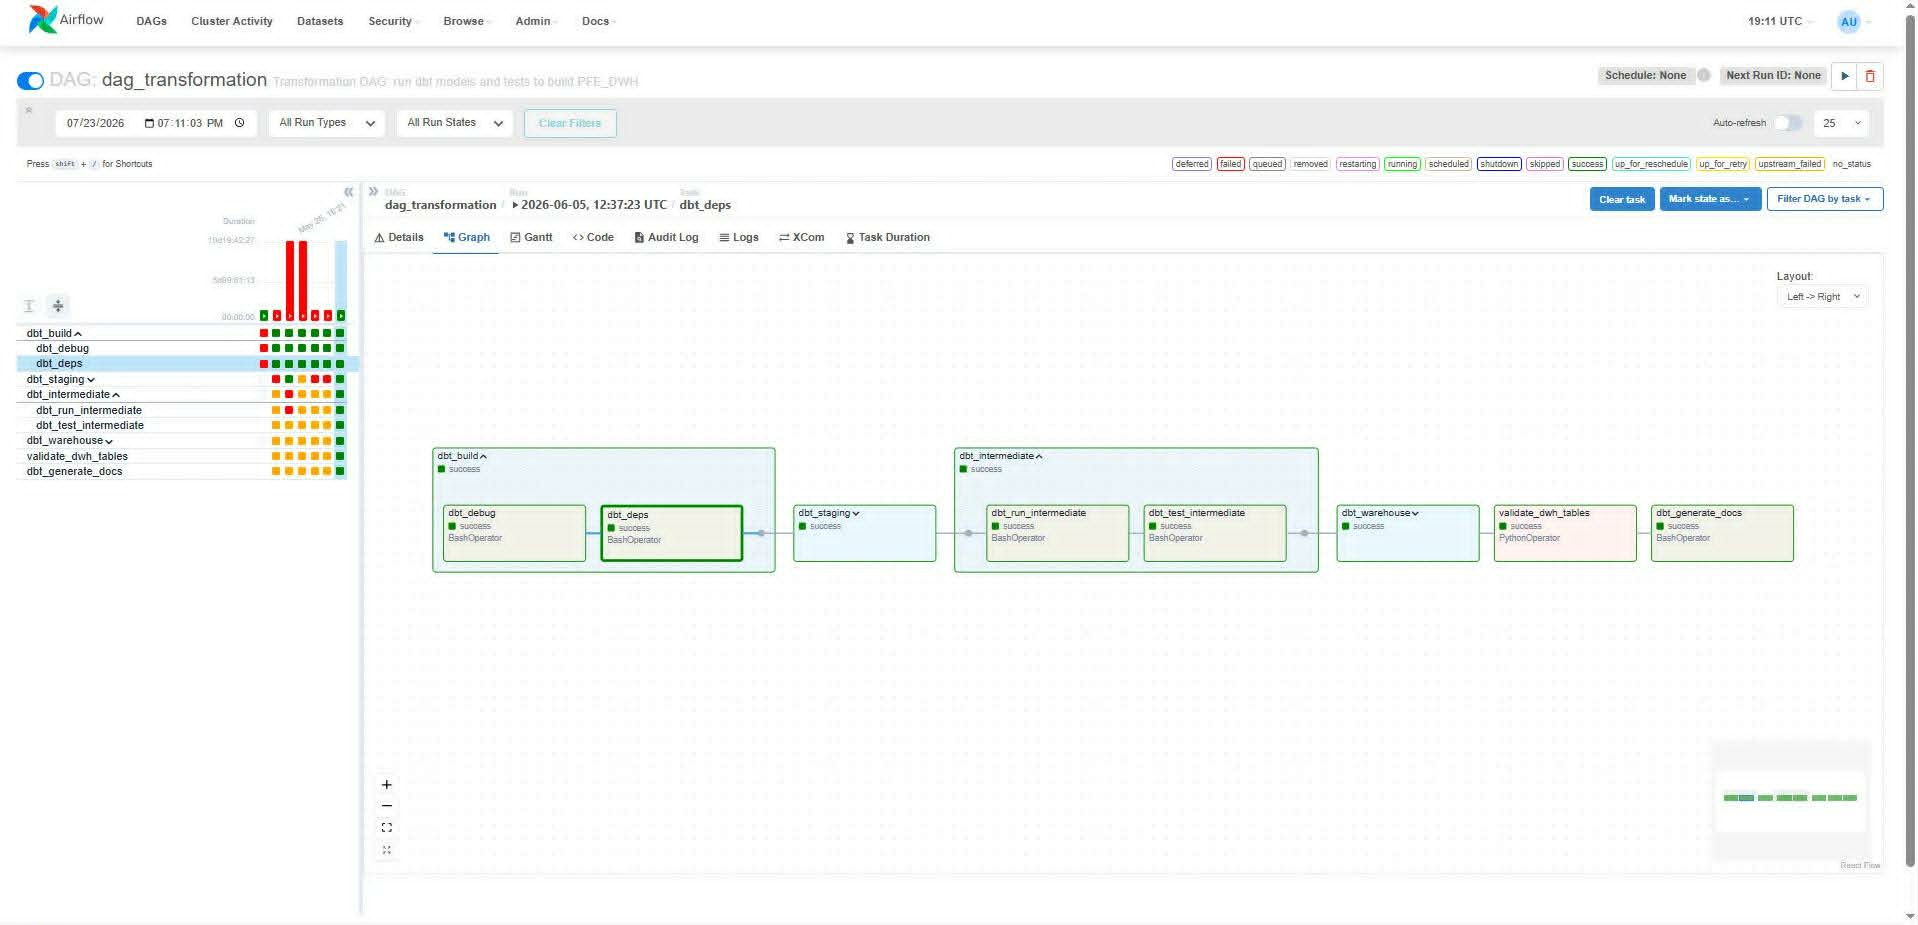
\includegraphics[width=0.9\textwidth]{figures/Full dag satus.png}
\caption{Full DAG status overview showing pipeline health across all runs}
\label{fig:full_dag_status}
\end{figure}

Beyond simple observation, the console also provides \textbf{direct control}. Three
action buttons allow authorised users to trigger a DAG manually for example, to force
a data refresh ahead of an important meeting as well as to pause or resume any
pipeline without ever leaving the Streamlit interface.

\begin{figure}[H]
\centering
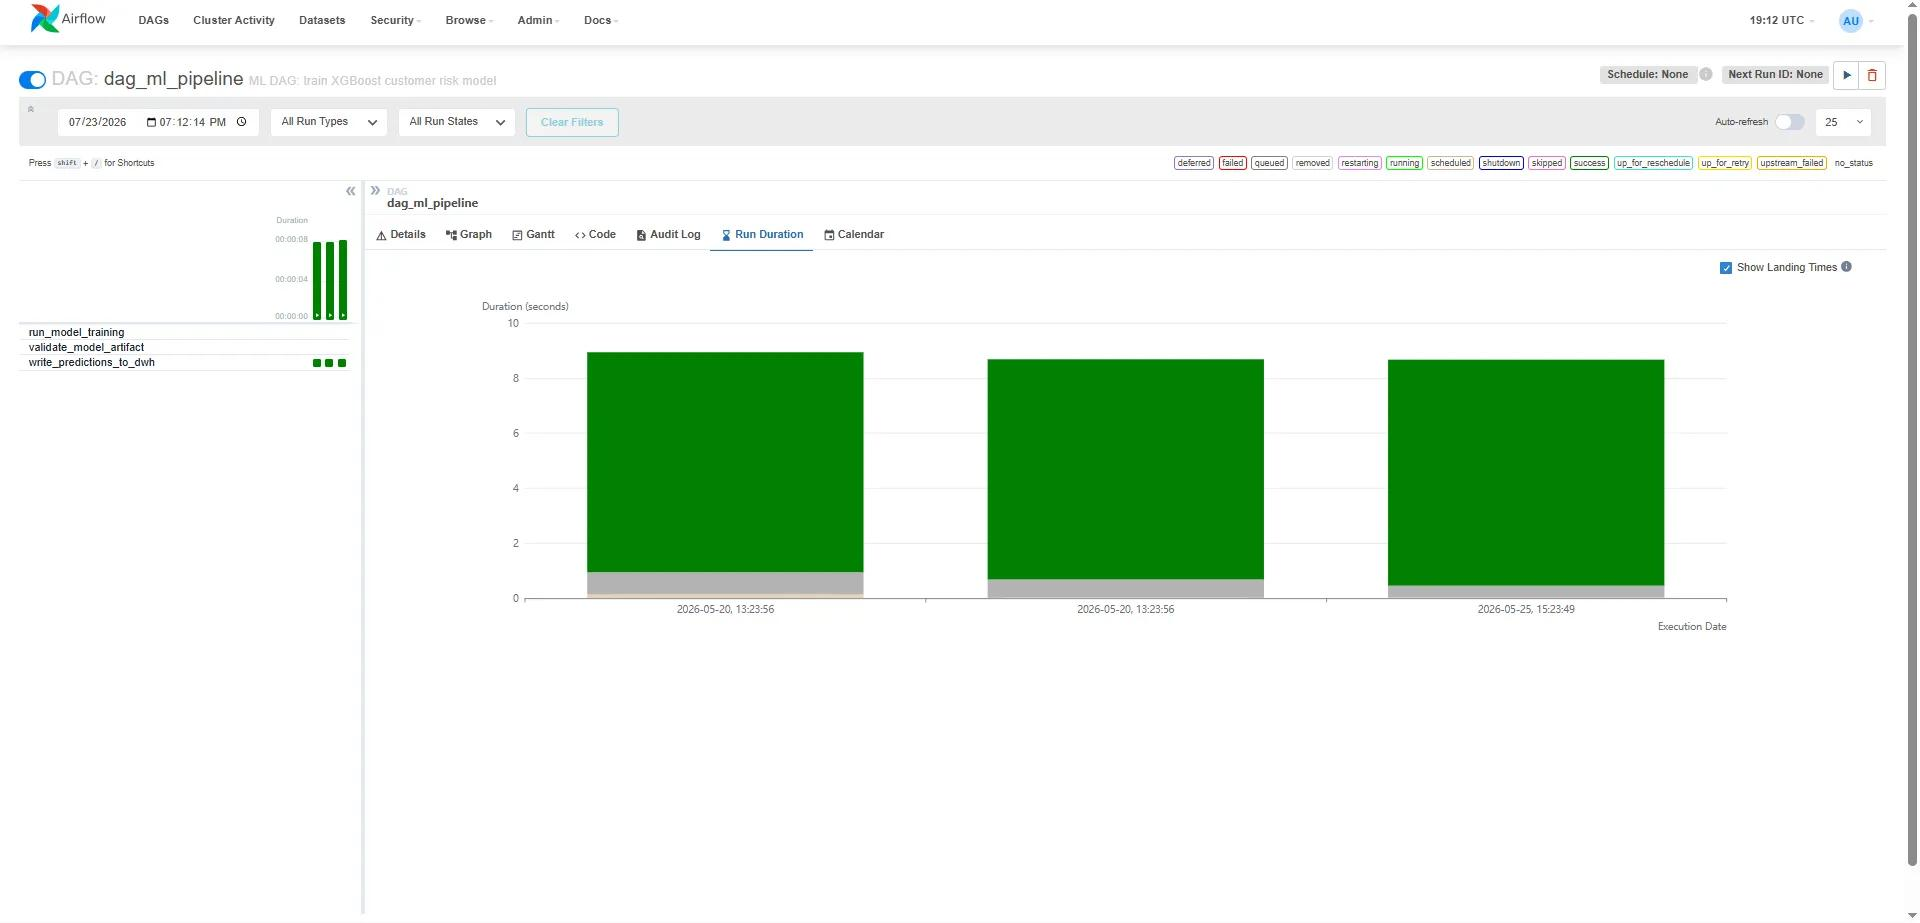
\includegraphics[width=0.9\textwidth]{figures/detailed dag action status.png}
\caption{Task-level detail view showing the outcome of each step within a DAG run}
\label{fig:detailed_dag_status}
\end{figure}

\begin{figure}[H]
\centering
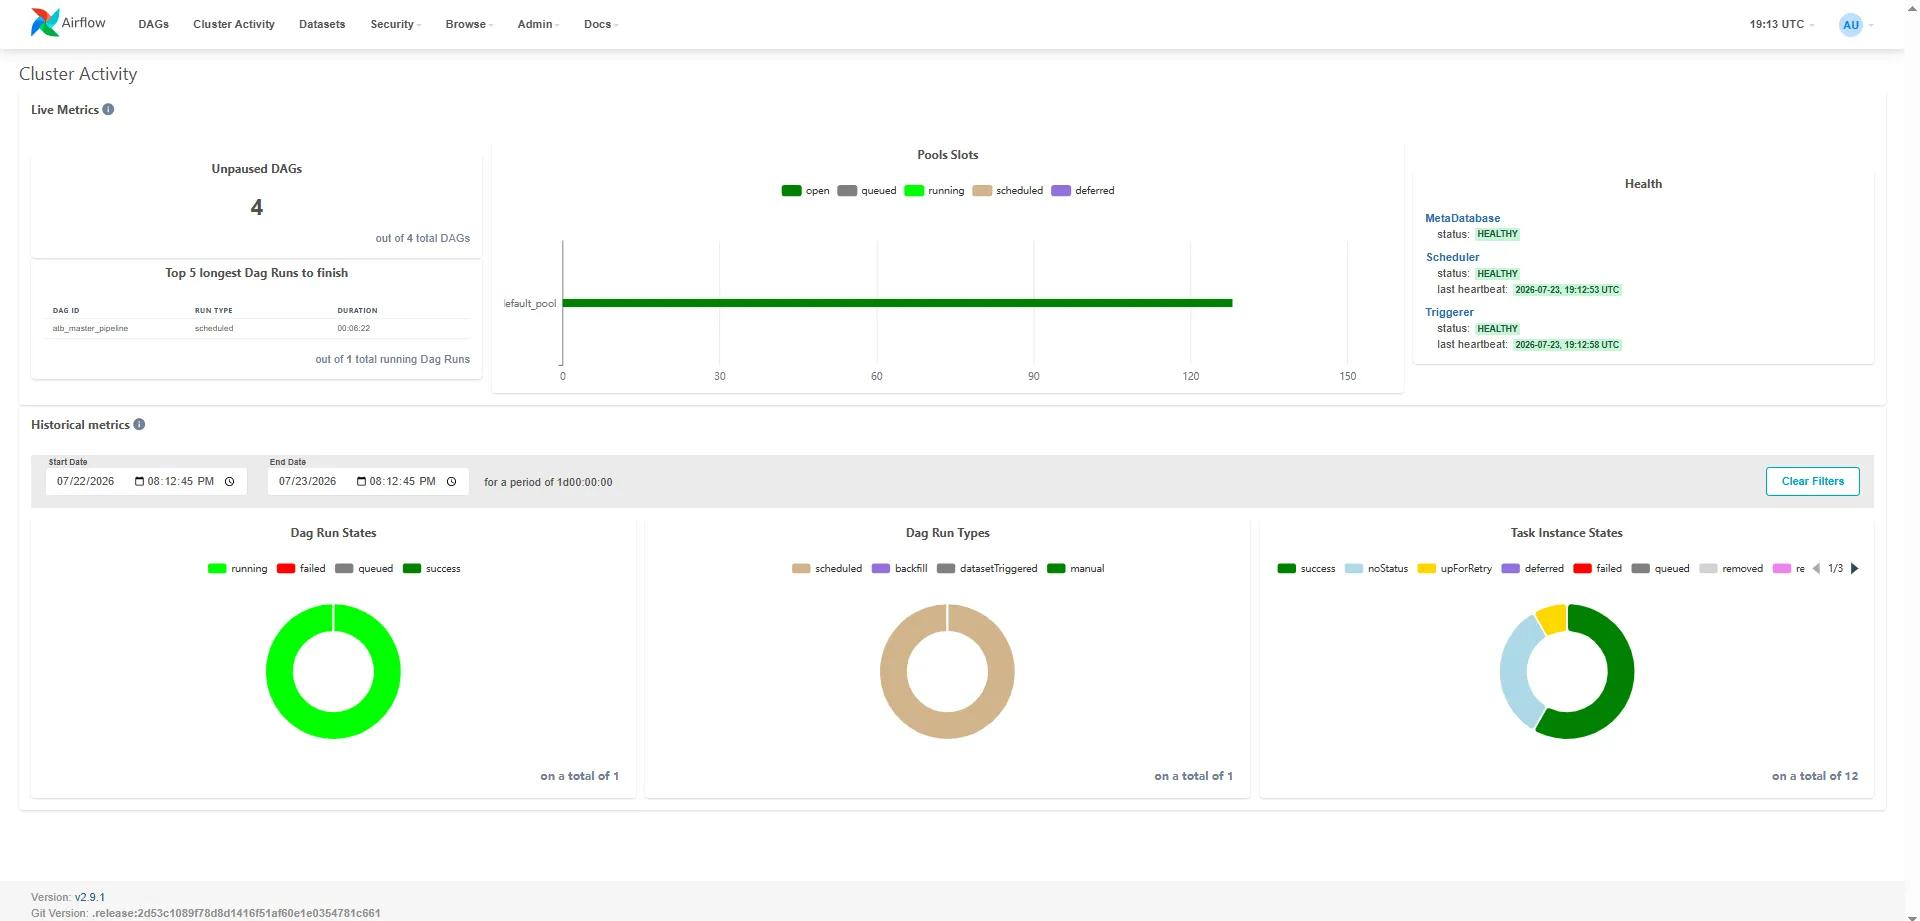
\includegraphics[width=0.9\textwidth]{figures/Airflow dashboard .png}
\caption{The Airflow web interface showing the graph view of the main pipeline}
\label{fig:airflow_webui}
\end{figure}

The same Operations Console also surfaces the status of the \textbf{underlying Docker
infrastructure}. A platform health card shows whether the Docker engine is accessible
and lists all running containers — the Airflow webserver, scheduler, triggerer, and
PostgreSQL database with their current state. Stack-level controls allow the
administrator to bring the entire Airflow stack up, down, or restart it, all through
the same unified interface. This means that the Streamlit dashboard is not merely a
reporting tool it is the central operational nerve centre of the entire data platform.

\subsubsection{Downstream Integration: From Data to Intelligence}

The pipeline does not end with data loading. Upon successful completion, it is
configured to automatically trigger the downstream machine learning pipeline, passing
control forward without any manual coordination. This creates a fully continuous,
end-to-end processing chain: raw source data enters on one side, and enriched,
ML-scored outputs emerge on the other all within a single nightly execution window,
while the organisation sleeps.

%------------------------------------------------
\section{Conclusion}

This first release established the engineering bedrock on which the entire ATB BI
platform rests. Rather than rushing toward dashboards and reports, the team invested
these two sprints in building something more fundamental: a platform that is secure
by design, autonomous by architecture, and reliable by construction.

Sprint 1 addressed the question of \textit{access}. By building a Streamlit interface
protected by role-based access control with passwords stored using salted SHA-256
hashing and user sessions scoped strictly to their organisational perimeter the
platform ensures that every interaction with banking data is authenticated,
authorised, and auditable.

Sprint 2 addressed the question of \textit{continuity}. The entire orchestration
infrastructure runs inside Docker containers, making the platform fully portable and
reproducible. Four complementary DAGs cover every aspect of the data lifecycle:
an end-to-end master pipeline that handles nightly warehouse loading and weekly
machine learning retraining, an on-demand ingestion DAG, an independent transformation
DAG, and a dedicated machine learning pipeline. The master pipeline coordinates nine
tasks across three task groups, executing every night at 02:00 UTC with a two-retry
fault-tolerance policy and integrated data quality checks that validate every foreign
key relationship before the data is made available to the business. A dedicated
monitoring panel embedded directly into the Streamlit dashboard gives authorised
administrators full real-time visibility and control over the entire platform without
ever leaving the application.
 
\textbf{Looking ahead to Release 2:} Building on this continuously operating,
autonomous foundation, the next release marks the moment where the platform
transitions from \textit{infrastructure} to \textit{intelligence}. Release 2 will
apply the GIMSI methodology to trace the complete business intelligence lifecycle:
how raw banking data extracted from seven source files travels through a rigorous
three-layer transformation process, is shaped into a governed analytical data warehouse,
and is finally brought to life on interactive Streamlit dashboards placing the right
indicators in front of the right decision-makers, at exactly the right moment.
%======================================================================
% CHAPTER 4 — RELEASE 2: BI INFRASTRUCTURE
% Skeleton aligned with supervisor-approved NotMyChapitre4 structure
% Content: ATB Customer Risk BI platform (Airbyte → dbt → PFE_DWH → Streamlit)
%======================================================================
\chapter{Release 2: Design and Implementation of the Business Intelligence Infrastructure}
\label{chap:release2}

%----------------------------------------------------------------------
\section{Introduction}
%----------------------------------------------------------------------
If Release~1 concentrated on deploying a secure operational software architecture
and an autonomous orchestration engine, this Release~2 marks a
fundamental transition toward analytical steering. The exclusive objective of
this phase encapsulated in Sprint~3: Consult the BI Dashboard
is to design and deploy a complete Business Intelligence (BI) infrastructure for
the decision-makers of the Arab Tunisian Bank (ATB): Central General Management,
the Chief Compliance Officer and Branch Managers.

Building a decision-support system obeys conceptual paradigms distinct from
classical transactional software development. The agile Scrum framework,
although maintained for overall project management, was therefore hybridised
with a data-engineering methodology. It is in this context that we adopted the
GIMSI methodology.

This chapter traces the full journey from raw pipe-separated banking extracts
to an interactive, role-aware Streamlit dashboard, through a Kimball
constellation warehouse and a transparent three-pillar customer risk score.

%======================================================================
\section{Methodological Framework: GIMSI}
\label{sec:gimsi_framework}
%======================================================================

\subsection{Functional Specification and Use Case Diagram of Sprint~3}
Sprint~3 is entirely dedicated to the development and deployment of the
ATB Decision Dashboard. It is the convergence point of every prior
architectural decision: the Airbyte ingestion pipeline, the dbt ELT models and
the Kimball constellation warehouse all serve a single output in this iteration a polished, role-aware Streamlit application consumed in real-time by ATB
decision-makers.

The major objective of this sprint is to offer bank decision-makers an
interactive, modern and visual decision-support tool that facilitates strategic
monitoring of customer risk, portfolio balances and regulatory compliance
alerts. Unlike traditional static reports, the dashboard evolves dynamically
with each nightly Airflow refresh, ensuring that every KPI card, chart and
compliance flag reflects yesterday's warehouse snapshot rather than last
month's Excel extract.

To frame the deliverables of this sprint and guarantee alignment with the
supervisors' expectations, we formulated a complete functional specification
before writing a single line of Streamlit code. This specification process
involved three structured steps. First, we identified the three actor profiles
Central General Management, the Chief Compliance Officer and Branch
Managers and documented their distinct analytical needs. Second, we
translated those needs into user stories (US~04 to US~09) and organised them
into a sprint backlog with priority ratings. Third, we validated the scope with
UML modelling, producing the use-case diagram presented hereafter
(Figure~\ref{fig:use_case_sprint3}), which serves as the contractual interface
between the development team and the stakeholders throughout the sprint.

This phase concentrates on exploiting and valorising the decision data
consolidated in the data warehouse during the preceding ELT phase. Through the
Streamlit application interface, each authorised user benefits from an overview
of portfolio activity via dynamic Plotly charts and Key Performance Indicators
(KPIs) computed directly from the warehouse facts. Role-based access control
(RBAC) ensures that Branch Managers operate in a strictly scoped view of their
own Desk Account Officer perimeter, while Central General Management retains a
cross-agency, national panorama.

With the functional scope fully specified and version-controlled, we can now
detail the interactions formalised in the use-case diagram below
(Figure~\ref{fig:use_case_sprint3}), which covers every actor and primary
behaviour supported during Sprint~3:

\begin{figure}[H]
\centering
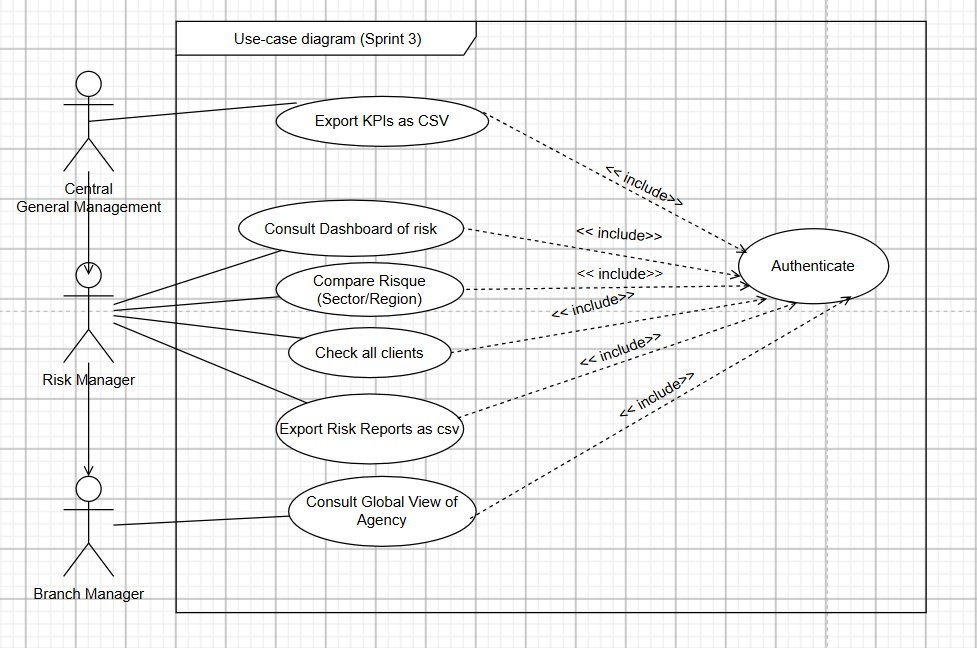
\includegraphics[width=0.9\textwidth]{figures/DiagramUseCaseSprint3.png}
\caption{Use-case diagram of the ATB Decision Dashboard (Sprint~3)}
\label{fig:use_case_sprint3}
\end{figure}

As illustrated, every actor interacts with the principal use case
\textbf{Consult the BI Dashboard}. Access requires authentication
(\textit{include}). Once connected, extended behaviours deepen the analysis:
\begin{itemize}
    \item \textbf{Visualisation of strategic KPIs:} synthetic follow-up of portfolio
          health (balances, average risk, overdraft rate).
    \item \textbf{Visualisation of Plotly charts:} dynamic exploration of risk tiers,
          sectors, industries and branches.
    \item \textbf{Branch-scoped filtering:} DAO restriction for Branch Managers
          (US~06).
    \item \textbf{Compliance watchlists:} PEP / KYC / flag queues for the Chief
          Compliance Officer.
    \item \textbf{AI chart explanations:} Gemini-generated textual readings with a
          deterministic template fallback.
    \item \textbf{Export of audit packs:} CSV and PDF extraction for committees
          (US~08).
\end{itemize}

Table~\ref{tab:sprint3_backlog} recalls the Sprint~3 product backlog (US~04 to
US~09) already defined in Chapter~2.

\begin{table}[H]
\centering
\caption{Product Backlog for Sprint~3 (Release~2)}
\label{tab:sprint3_backlog}
\renewcommand{\arraystretch}{1.35}
\resizebox{\textwidth}{!}{%
\begin{tabular}{|c|c|p{3.0cm}|p{5.6cm}|p{4.0cm}|}
\hline
\rowcolor{blue!15}
\textbf{ID} & \textbf{Priority} & \textbf{As a\ldots} & \textbf{I want to\ldots} & \textbf{So that\ldots} \\
\hline
\textbf{US 04} & High & Central GM & extract and load sources via Airbyte & ODS is fed without manual copy. \\
\hline
\textbf{US 05} & High & Central GM & define and calculate risk KPIs in the DWH & portfolio health uses shared audited formulas. \\
\hline
\textbf{US 06} & High & Branch Manager & consult my agency's filtered Streamlit view & I monitor local risk without seeing other branches. \\
\hline
\textbf{US 07} & High & Central GM & analyse indicators for all agencies nationally & I compare regions and risk concentrations. \\
\hline
\textbf{US 08} & High & Central GM & export management indicators as CSV/PDF & audit packs can leave the tool. \\
\hline
\textbf{US 09} & Low & Risk Manager & track customer history across agencies & score evolution remains visible over time. \\
\hline
\end{tabular}%
}
\end{table}

\subsection{Application of GIMSI to Sprint~3}
To meet Release~2 requirements, the software architecture of the platform was
rigorously mapped onto the four GIMSI pillars. Table~\ref{tab:gimsi_phases}
illustrates the exact cartography between the theoretical GIMSI framework, BI
architecture concepts and the technical implementations realised in this sprint.
Figure~\ref{fig:gimsi_cycle_atb} summarises the cycle graphically.

\begin{figure}[H]
\centering
\begin{tikzpicture}[
  font=\small,
  phase/.style={rectangle, rounded corners=3pt, draw=#1, fill=#1!12, thick,
                align=center, minimum width=3.6cm, minimum height=1.55cm},
  arr/.style={->, very thick, gray!60}
]
  \node[phase=teal!70!black] (p1) at (0,2.4) {\textbf{1. Identification}\\Requirements +\\Airbyte ODS};
  \node[phase=blue!70!black] (p2) at (5.2,2.4) {\textbf{2. Design}\\Kimball constellation\\+ KPI specification};
  \node[phase=violet!70!black] (p3) at (5.2,0.0) {\textbf{3. Realisation}\\dbt ELT + DWH\\+ Streamlit};
  \node[phase=orange!80!black] (p4) at (0,0.0) {\textbf{4. Evaluation}\\Airflow freshness\\+ continuous audit};
  \draw[arr] (p1) -- (p2);
  \draw[arr] (p2) -- (p3);
  \draw[arr] (p3) -- (p4);
  \draw[arr] (p4) -- (p1);
\end{tikzpicture}
\caption{GIMSI cycle applied to the ATB BI Release~2}
\label{fig:gimsi_cycle_atb}
\end{figure}

\begin{table}[H]
\centering
\caption{Cartography of the GIMSI methodology applied to the ATB BI architecture}
\label{tab:gimsi_phases}
\renewcommand{\arraystretch}{1.25}
\scriptsize
\begin{tabular}{|p{2.6cm}|p{4.0cm}|p{7.4cm}|}
\hline
\rowcolor{blue!15}
\textbf{GIMSI Phase} & \textbf{BI Architecture Concept} & \textbf{Implementation in Sprint~3} \\
\hline
\textbf{1. Identification} & Requirements model \& source acquisition & Actors DG / Compliance / Branch; FR/NFR; seven pipe-separated CSVs synchronised by Airbyte into \texttt{PFE\_ODS}. \\
\hline
\textbf{2. Design} & Dimensional modelling & Kimball constellation (8 dimensions + 2 facts); mathematical definition of portfolio and risk KPIs; visual dashboard specification. \\
\hline
\textbf{3. Realisation} & Access, Warehouse, Business \& Presentation layers & dbt ELT (staging / intermediate / warehouse), three-pillar scoring, SQL Server \texttt{PFE\_DWH}, Streamlit RBAC dashboard. \\
\hline
\textbf{4. Evaluation} & Freshness \& continuous improvement & Airflow nightly schedule (\texttt{0 2 * * *}), Streamlit TTL cache, dbt tests, KPI evolution roadmap. \\
\hline
\end{tabular}
\end{table}

%======================================================================
\section{Phase 1: Identification}
\label{sec:gimsi_phase1}
%======================================================================
The first phase aims to understand the context, inventory dashboard requirements,
and identify and extract the raw data that will feed the warehouse.

\subsection{The Requirements Model}
The requirements model is a design artefact used to document the expectations of
ATB decision-makers. It clarified the functionalities that the BI layer must
deliver:
\begin{itemize}
    \item obtain instant visibility on portfolio balances and average customer risk;
    \item isolate profiles requiring urgent compliance or credit follow-up
          (PEP, incomplete KYC, high Global Risk Score);
    \item analyse distributions by sector, industry, employment and branch area;
    \item enforce branch segregation so that a local manager never sees another
          agency's book.
\end{itemize}

\paragraph{Identified actors.}
\begin{itemize}
    \item \textbf{Central General Management:} macroscopic
          national view, cross-agency comparison, export for committees.
    \item \textbf{Chief Compliance Officer:} KYC/PEP
          watchlists, compliance flags, alert inbox.
    \item \textbf{Branch Manager:} same analytical language,
          restricted to the Desk Account Officer (DAO) / branch perimeter.
\end{itemize}

\paragraph{Functional Requirements (FR).}
\begin{itemize}
    \item \textbf{FR1 --- Portfolio KPIs:} display aggregated indicators (customers,
          accounts, total balance, average risk, overdraft share).
    \item \textbf{FR2 --- Risk profiling:} compute a daily classification into
          \texttt{LOW} / \texttt{MEDIUM} / \texttt{HIGH} / \texttt{VERY\_HIGH}.
    \item \textbf{FR3 --- Branch segregation:} filter analytical outputs by DAO area
          for Branch Managers.
    \item \textbf{FR4 --- Watchlist audit:} expose PEPs, incomplete KYC and overdue
          review dates.
    \item \textbf{FR5 --- Detail inspection:} open a customer fiche with the
          three-pillar breakdown (CRI, FFS, BRS).
    \item \textbf{FR6 --- Explainable insights:} provide AI-generated chart
          explanations to support reading during committees.
\end{itemize}

\paragraph{Non-Functional Requirements (NFR).}
\begin{itemize}
    \item \textbf{NFR1 --- Row-level security:} SQL filters injected from the session
          (\texttt{dao\_filter\_sql()}).
    \item \textbf{NFR2 --- Render latency:} interactive pages respond in under
          $\approx 2$~s in normal use.
    \item \textbf{NFR3 --- Access efficiency:} SQLAlchemy connection pooling and
          Streamlit result caching.
    \item \textbf{NFR4 --- Referential integrity:} $100\%$ fact foreign keys resolved
          (sentinel UNKNOWN rows; zero NULL FKs).
    \item \textbf{NFR5 --- Traceability:} every transformation versioned in Git and
          covered by dbt tests.
\end{itemize}

Table~\ref{tab:fr_nfr_traceability} cross-references requirements to Sprint~3
user stories and technical components --- a traceability artefact required for
academic and audit readability.

\begin{table}[H]
\centering
\caption{Requirements-to-implementation traceability matrix}
\label{tab:fr_nfr_traceability}
\renewcommand{\arraystretch}{1.2}
\scriptsize
\begin{tabular}{|c|p{4.2cm}|c|p{5.5cm}|}
\hline
\rowcolor{blue!15}
\textbf{Req.} & \textbf{Intent} & \textbf{US} & \textbf{Technical realisation} \\
\hline
FR1 & Portfolio KPI cards & US~05, US~07 & \texttt{loaders.load\_executive\_kpis()} on \texttt{fact\_*} \\
\hline
FR2 & Daily risk tiers & US~05 & \texttt{int\_customer\_risk\_score} $\rightarrow$ \texttt{fact\_customer\_risk} \\
\hline
FR3 & Branch segregation & US~06 & RBAC + \texttt{dao\_filter\_sql()} \\
\hline
FR4 & PEP / KYC watchlists & US~05 & Compliance + Alert inbox pages \\
\hline
FR5 & Three-pillar fiche & US~05, US~09 & Risk page + \texttt{dim\_risk\_profile} \\
\hline
FR6 & AI explanations & US~07 & Gemini explainer + template fallback \\
\hline
NFR1 & Row-level security & US~06 & Session-scoped SQL WHERE \\
\hline
NFR4 & Zero NULL FKs & US~05 & Sentinel $-1$ / \texttt{UNK} + \texttt{COALESCE} \\
\hline
NFR5 & Tested lineage & US~04, US~05 & Airbyte $\rightarrow$ dbt tests $\rightarrow$ Airflow DQ \\
\hline
\end{tabular}
\end{table}

\subsection{Data Source Acquisition (Airbyte on Docker, Hosted via GitHub)}
In practice, a BI project is only as trustworthy as the way raw files enter the
system. ATB provided seven pipe-separated (\texttt{|}) CSV extracts from the core
banking environment. Rather than copying them by hand into SQL Server, we built
a small but realistic enterprise pattern: \textbf{publish the files once, sync
them automatically forever}.

\paragraph{GitHub as a Data Host}
The CSV extracts were published under the project repository path
\texttt{data/raw/}. GitHub then acts as a lightweight, versioned file host:
each raw file is reachable through a stable HTTPS raw URL that Airbyte can
poll. This choice has three practical advantages for a PFE deployment:
\begin{itemize}
    \item \textbf{Version control:} every change to a source extract is committed
          and auditable;
    \item \textbf{No local path fragility:} Airbyte does not depend on a Windows
          folder that may move or disappear;
    \item \textbf{Repeatable demos:} anyone with repository access can rebuild the
          same ingestion from the same published URLs.
\end{itemize}

\paragraph{Airbyte running in Docker.}
Airbyte itself is deployed as a \textbf{Docker} stack (containers for the web UI,
workers and temporal services). From the browser UI we created seven
\textbf{HTTPS / File} source connectors one per CSV pointing to those
GitHub raw URLs. For each connector we configured:
\begin{itemize}
    \item format \texttt{csv}, delimiter \texttt{|}, header row enabled;
    \item explicit column dtypes (strings for codes, floats for balances/salary);
    \item a destination dataset name in the ODS
          (\texttt{ODS\_CUSTOMER}, \texttt{ODS\_ACCOUNT}, \texttt{ODS\_DAO},\ldots).
\end{itemize}
The destination connector targets Microsoft SQL Server, schema
\texttt{PFE\_ODS}, database \texttt{ATB\_BI}. After a successful sync, the ODS
contains a faithful mirror of the GitHub files, enriched with Airbyte technical
columns such as \texttt{\_airbyte\_raw\_id} and \texttt{\_airbyte\_extracted\_at}.

Figure~\ref{fig:airbyte_ingest_flow} formalises this chain.
\begin{figure}[H]
\centering
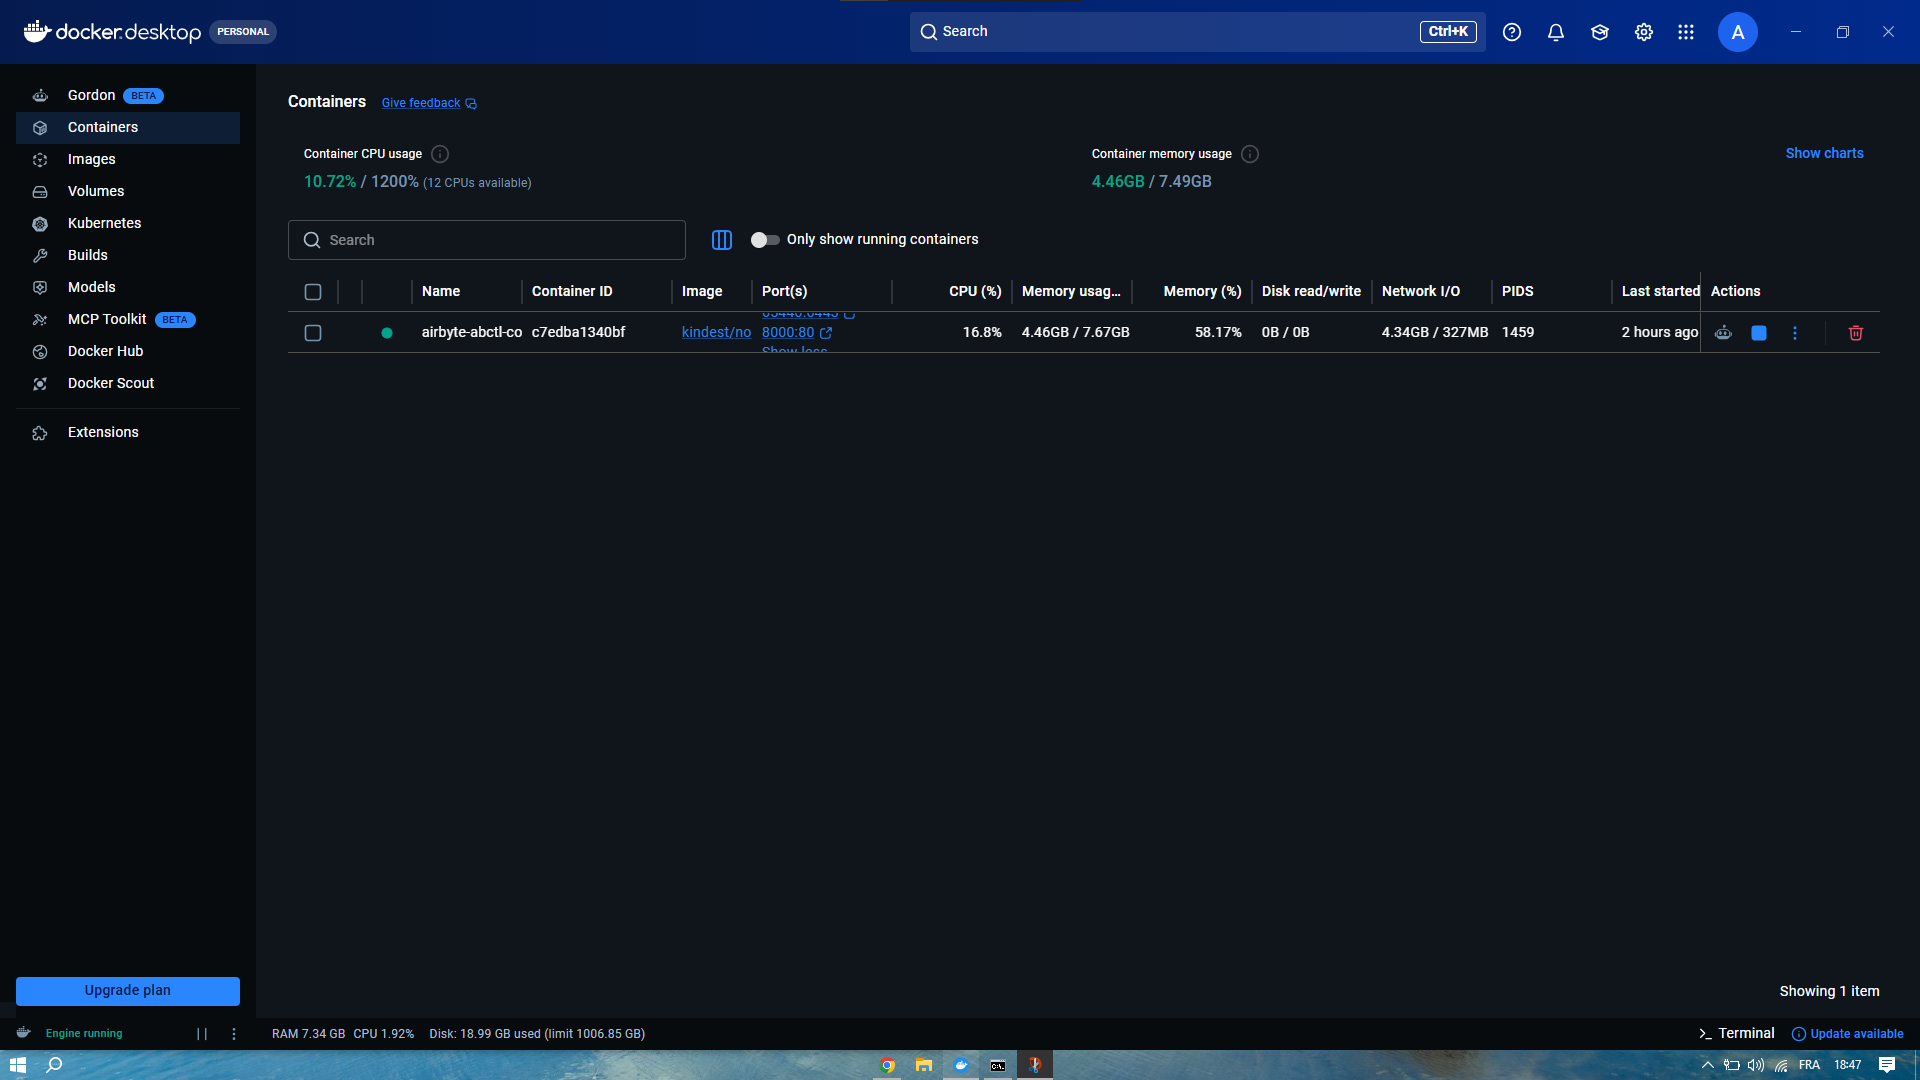
\includegraphics[width=0.85\textwidth]{figures/airbyte_docker_ui.png}
\caption{Airbyte UI home / workspace running in Docker}
\label{fig:airbyte_docker_ui}
\end{figure}
The Docker-hosted Airbyte workspace is the operational control plane from which all seven
CSV sources and the SQL Server destination are configured.

\begin{figure}[H]
\centering
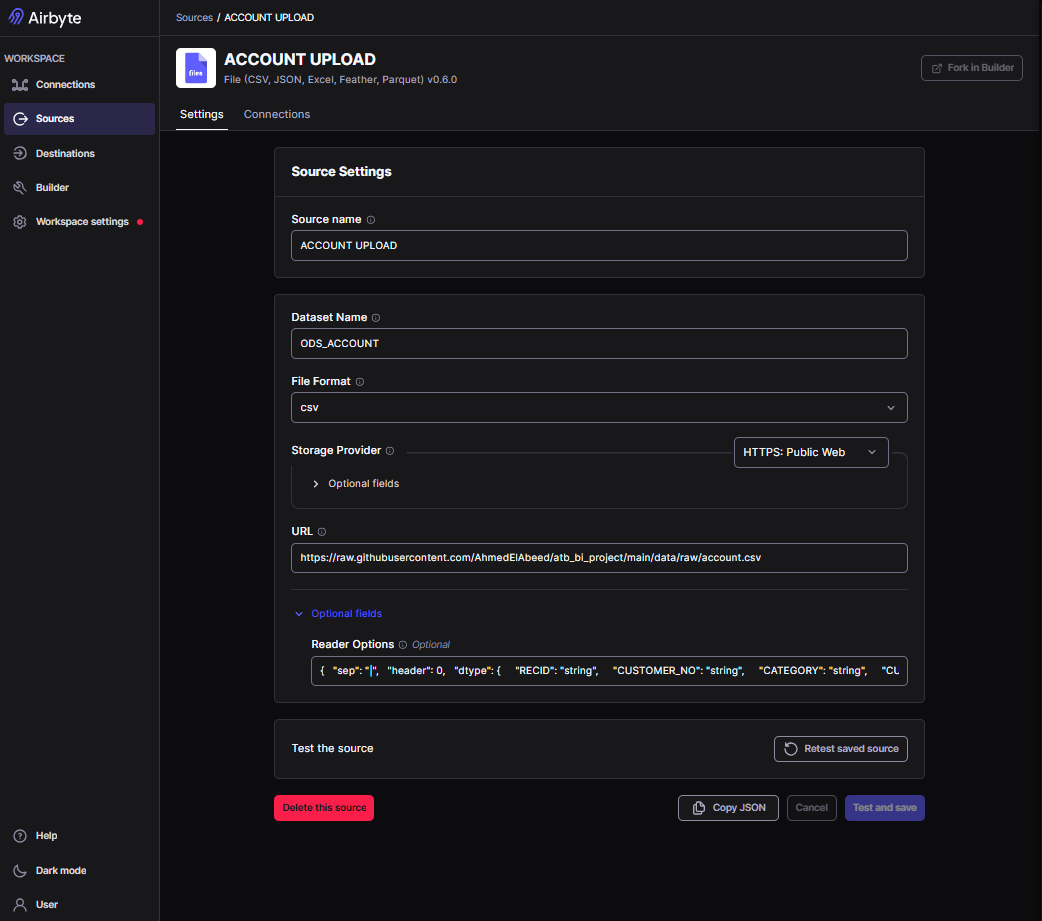
\includegraphics[width=0.7\textwidth]{figures/airbyte_github_source.png}
\caption{HTTPS source connector pointing to the GitHub raw CSV URL}
\label{fig:airbyte_github_source}
\end{figure}
Each source connector reads a pipe-delimited extract over HTTPS, avoiding fragile local
file paths on the developer workstation.

\begin{figure}[H]
\centering
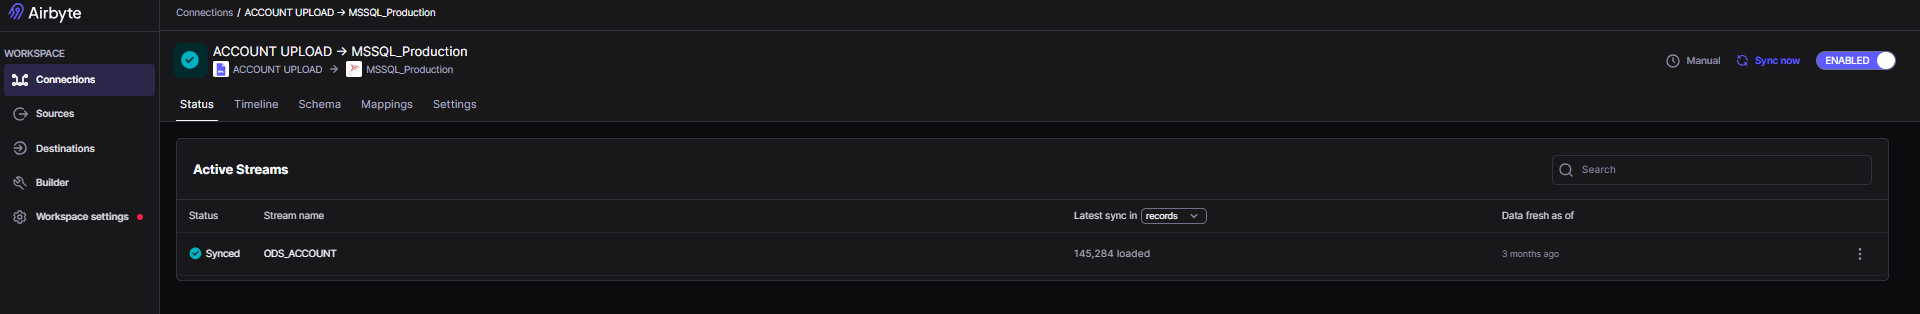
\includegraphics[width=0.85\textwidth]{figures/airbyte_connections_list.png}
\caption{List of the 7 Airbyte sync connections}
\label{fig:airbyte_connections_list}
\end{figure}
The connection list mirrors the seven raw datasets and makes sync status visible at a
glance before any dbt transformation runs.

\begin{figure}[H]
\centering
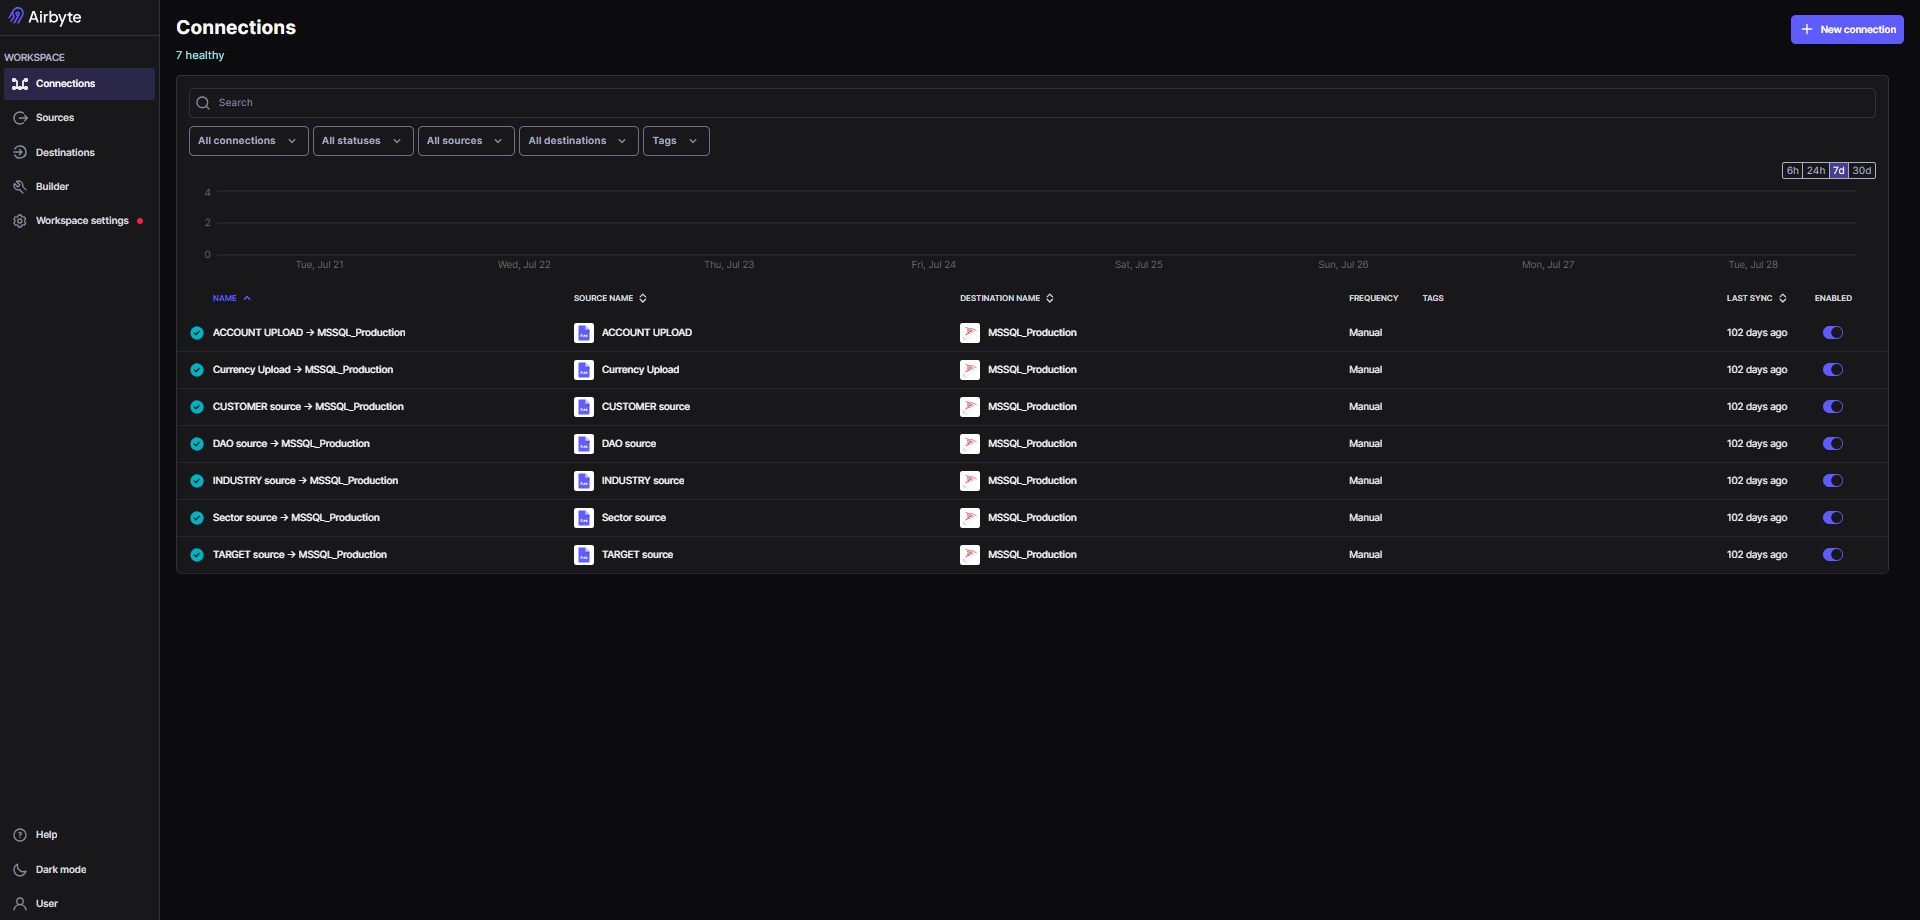
\includegraphics[width=0.85\textwidth]{figures/airbyte_sync_success.png}
\caption{Successful Airbyte sync job green status after loading into Database}
\label{fig:airbyte_sync_success}
\end{figure}
A green sync confirms that the ODS tables were refreshed and are ready for staging models.

\begin{figure}[H]
\centering
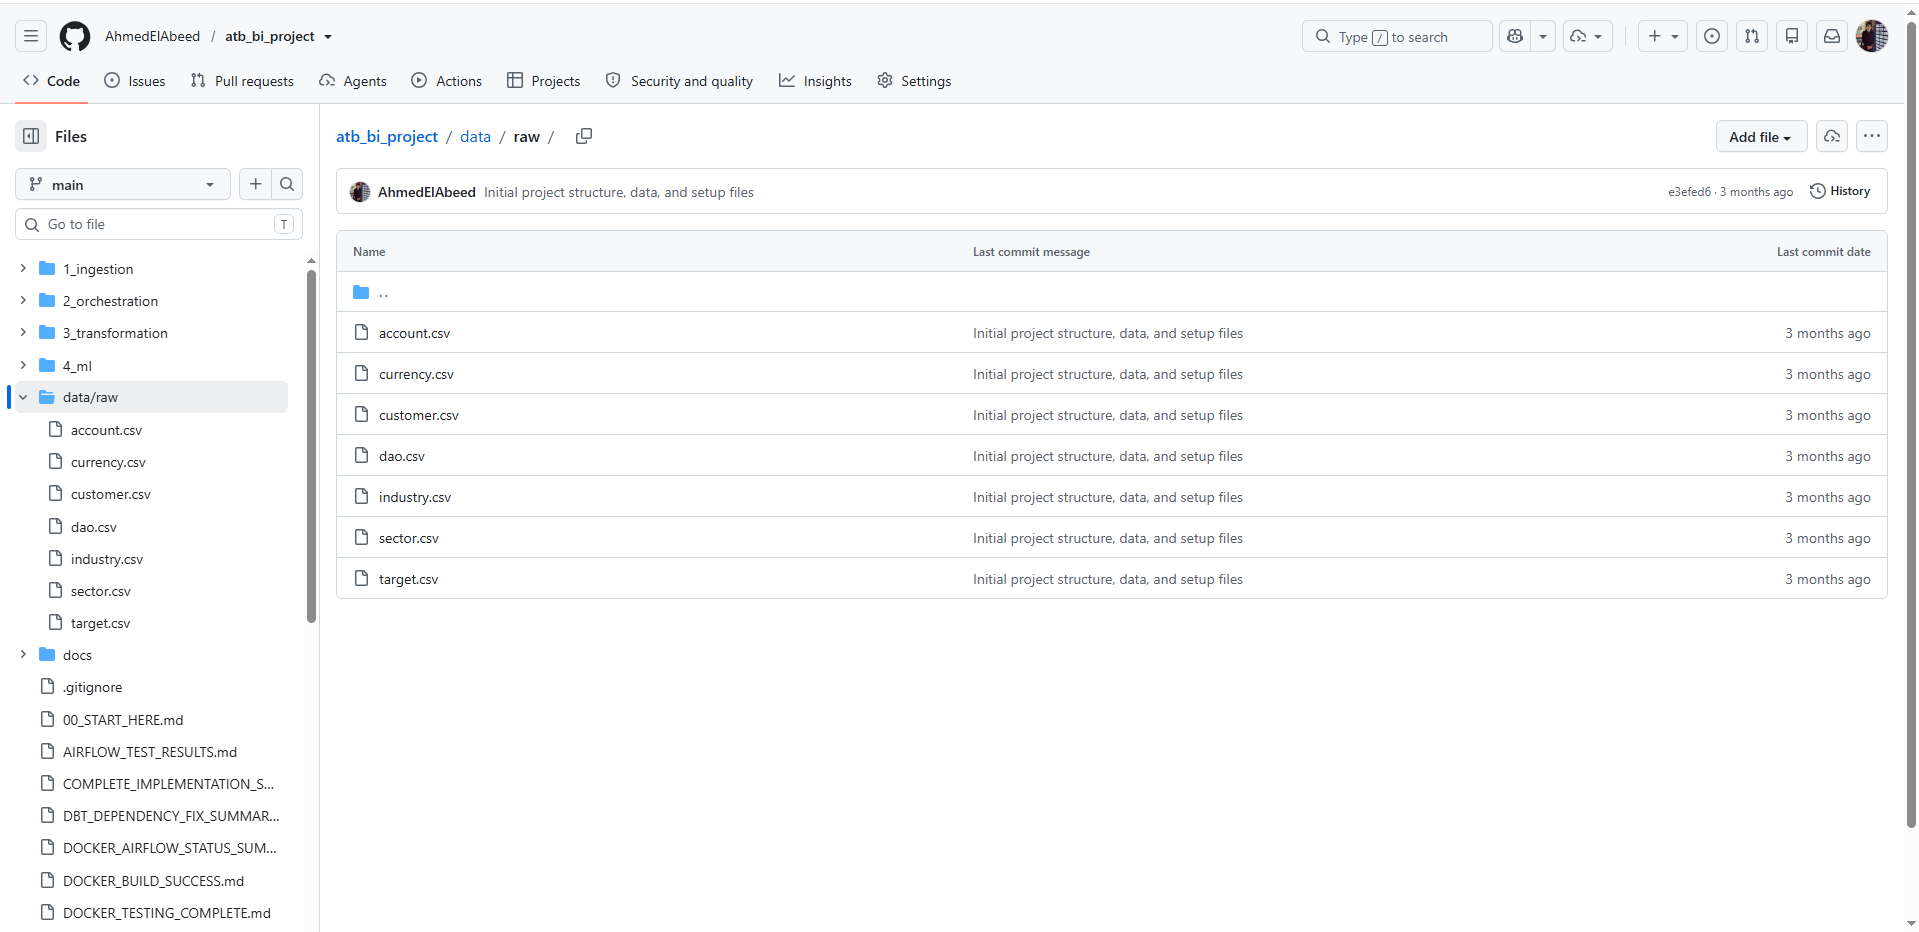
\includegraphics[width=0.85\textwidth]{figures/github_raw_csv.png}
\caption{GitHub repository view of raw CSV files in \texttt{data/raw/}}
\label{fig:github_raw_csv}
\end{figure}
Versioned extracts under \texttt{data/raw/} provide a single, auditable source location
for every Airbyte HTTPS connector.

\begin{figure}[H]
\centering
\begin{tikzpicture}[
  font=\scriptsize,
  box/.style={rectangle, rounded corners=2pt, draw=#1, fill=#1!10, thick,
              align=center, minimum width=2.45cm, minimum height=1.2cm},
  arr/.style={->, thick}
]
  \node[box=gray!70!black] (csv) {7 CSV files\\uploaded to GitHub};
  \node[box=orange!75!black, right=0.4cm of csv] (gh) {GitHub raw\\HTTPS URLs};
  \node[box=cyan!70!black, right=0.4cm of gh] (ab) {Airbyte\\(Docker)};
  \node[box=blue!70!black, right=0.4cm of ab] (ods) {\texttt{PFE\_ODS}\\SQL Server};
  \draw[arr] (csv) -- (gh);
  \draw[arr] (gh) -- (ab);
  \draw[arr] (ab) -- (ods);
\end{tikzpicture}
\caption{Source acquisition chain GitHub-hosted CSVs synchronised by Airbyte (Docker) into \texttt{ODS}}
\label{fig:airbyte_ingest_flow}
\end{figure}

\begin{figure}[H]
\centering
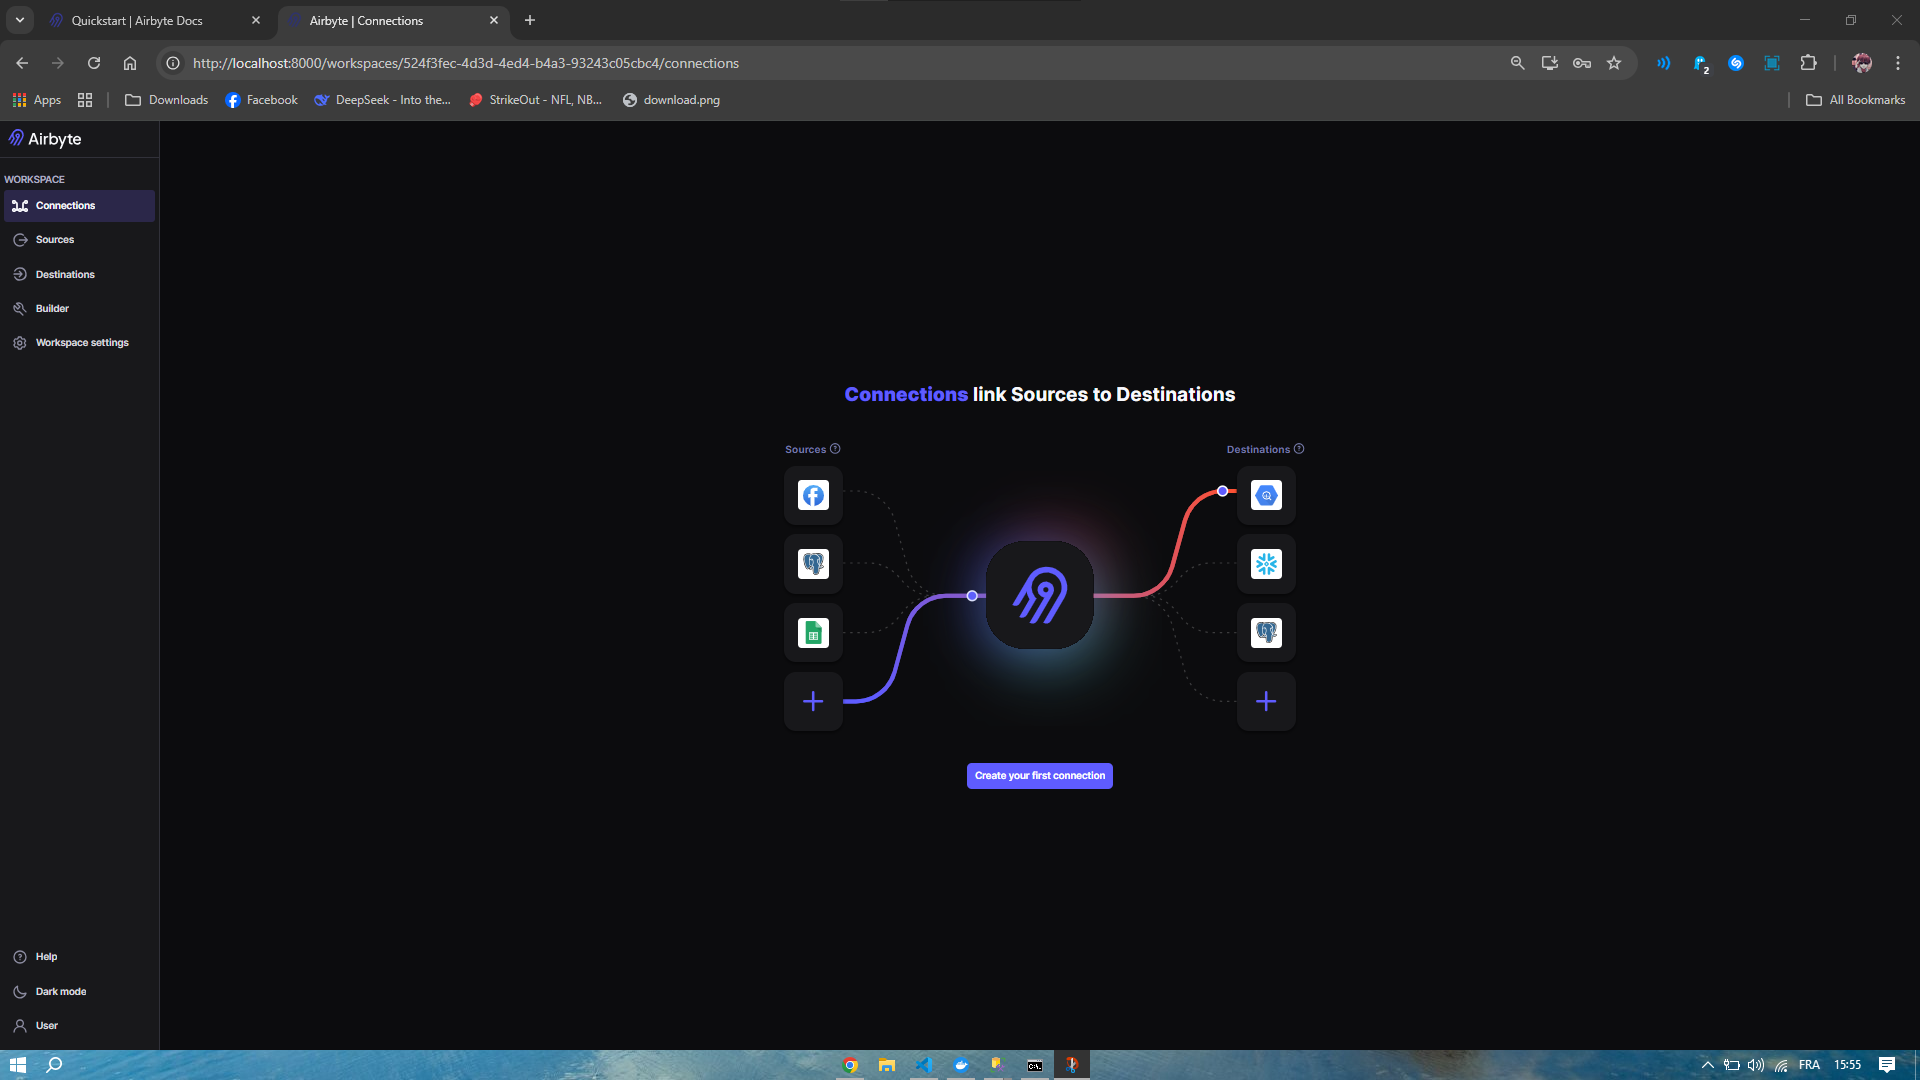
\includegraphics[width=0.55\textwidth]{figures/Airbyte_plateform.png}
\caption{Airbyte platform used as the ingestion engine of Release~2}
\label{fig:airbyte_logo_ref}
\end{figure}

Table~\ref{tab:raw_volumes} registers the measured volumes after a successful
sync. These counts later reappear almost one-to-one in the warehouse facts a
simple but reassuring integrity check.

\begin{table}[H]
\centering
\caption{Detailed volumetry of source datasets ingested by Airbyte}
\label{tab:raw_volumes}
\renewcommand{\arraystretch}{1.25}
\scriptsize
\begin{tabular}{|p{2.8cm}|c|c|p{7.0cm}|}
\hline
\rowcolor{blue!15}
\textbf{Source CSV} & \textbf{Rows} & \textbf{ODS table} & \textbf{Business content} \\
\hline
\texttt{customer.csv} & $136{,}676$ & \texttt{ODS\_CUSTOMER} & Identity, employment, salary, KYC/PEP/compliance flags, DAO link. \\
\hline
\texttt{account.csv} & $145{,}284$ & \texttt{ODS\_ACCOUNT} & Working balances, opening dates, currency, officer link. \\
\hline
\texttt{dao.csv} & $150$ & \texttt{ODS\_DAO} & Desk Account Officers, branch areas and names. \\
\hline
\texttt{currency.csv} & $22$ & \texttt{ODS\_CURRENCY} & ISO currency reference. \\
\hline
\texttt{sector.csv} & $45$ & \texttt{ODS\_SECTOR} & Macro-economic sectors. \\
\hline
\texttt{industry.csv} & $663$ & \texttt{ODS\_INDUSTRY} & Detailed activity codes. \\
\hline
\texttt{target.csv} & $11$ & \texttt{ODS\_TARGET} & Client segments (retail, SME, corporate,\ldots). \\
\hline
\end{tabular}
\end{table}

In plain words: GitHub stores the files, Docker runs Airbyte, SQL Server receives
the ODS tables, and Airflow later triggers the same syncs every night. That is
the ingestion backbone behind US~04.

%======================================================================
\section{Phase 2: Design}
\label{sec:gimsi_phase2}
%======================================================================
The second GIMSI phase translates decision-maker needs into measurable indicators
and designs the data model that will compute them.

\subsection{Design Methodology: Kimball Approach and Dimensional Modelling}
The physical modelling of the decision warehouse relies rigorously on the
dimensional modelling concepts theorised by Ralph Kimball \cite{kimball2013}.
This approach pursues two essential objectives in decision engineering:
facilitate intuitive data exploration for business users, and optimise analytical
query performance by limiting join complexity.

\paragraph{Conformed dimensions and surrogate keys.}
The constellation structure rests on sharing \textbf{conformed dimensions}
across business processes. These dimensions constitute the unique, standardised
referential of the warehouse:
\begin{itemize}
    \item \texttt{dim\_customer} --- demographics, tenure, KYC/PEP/compliance attributes;
    \item \texttt{dim\_dao} --- account officer and branch/area mapping;
    \item \texttt{dim\_date} --- calendar attributes for openings and scoring dates;
    \item \texttt{dim\_sector}, \texttt{dim\_industry}, \texttt{dim\_target} ---
          economic and commercial segmentation;
    \item \texttt{dim\_currency} --- ISO codes plus an \texttt{UNK} sentinel;
    \item \texttt{dim\_risk\_profile} --- historical three-pillar scores per scoring date.
\end{itemize}

Referential integrity is guaranteed by \textbf{surrogate keys} (e.g.\
\texttt{customer\_sk}, \texttt{dao\_sk}). Each dimension holds a system-generated
integer identifier independent of volatile source business keys. This isolates
the warehouse from upstream key changes and accelerates SQL joins required by
visual restitutions.

\paragraph{Fact tables and constellation (galaxy) structure.}
The ATB constellation materialises through two complementary fact tables connected
to the conformed dimensions:
\begin{itemize}
    \item \texttt{fact\_account} --- transactional balance snapshot (grain: one row
          per account);
    \item \texttt{fact\_customer\_risk} --- scored risk profile (grain: one row per
          customer per scoring date).
\end{itemize}
Crossing both facts via shared dimensions (customer, DAO, sector,\ldots) enables
advanced analyses such as: \emph{average risk of overdrawn accounts in the Tunis
Centre area, by industry}.

\paragraph{Bottom-up architecture and agile integration.}
Contrary to Bill Inmon's top-down 3NF enterprise warehouse --- complex to deploy
up-front --- we adopted Kimball's \textbf{bottom-up} architecture:
\begin{itemize}
    \item \textbf{Incremental agile delivery:} Release~1 prepared orchestration and
          security; Release~2 grafts the constellation and dashboard without
          destabilising the foundation, matching the Scrum sprint cadence.
    \item \textbf{Performance through controlled denormalisation:} limiting join
          depth is essential for fast Plotly rendering on Streamlit.
\end{itemize}

\subsection{Dimensional Modelling: Constellation Schema}
Figure~\ref{fig:galaxy_schema_ref} shows the production constellation diagram;
Figure~\ref{fig:constellation_tikz} abstracts the same model as a TikZ schematic
for academic clarity.

\begin{figure}[H]
\centering
\includegraphics[width=0.82\textwidth]{figures/galaxy_schema.png}
\caption{ATB Kimball constellation schema  conformed dimensions shared by
Both fact tables}
\label{fig:galaxy_schema_ref}
\end{figure}

\begin{figure}[H]
\centering
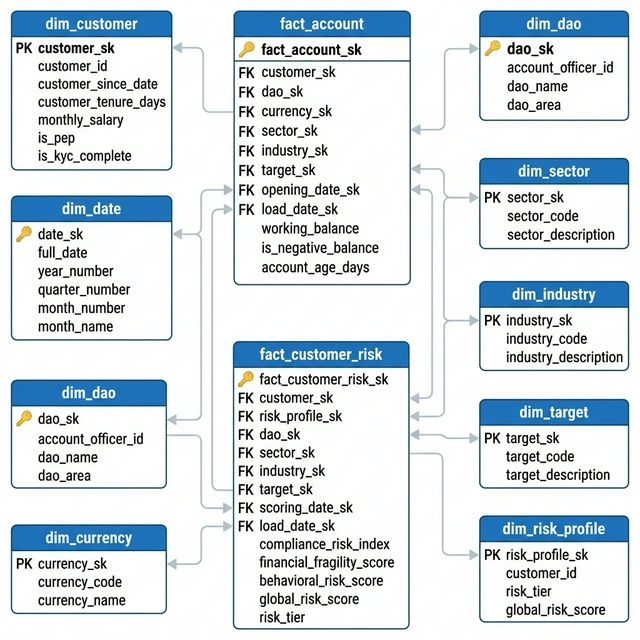
\includegraphics[width=0.85\textwidth]{figures/constellation view model.png}
\caption{Abstract constellation view shared conformed dimensions around two facts}
\label{fig:constellation_tikz}
\end{figure}

\paragraph{Reuse of engineered features in the BI dashboard.}
Variables produced in the intermediate dbt layer (pillar scores, account
aggregates, tenure, overdraft flags) are not reserved for Machine Learning. They
constitute the \textbf{computational substrate of the BI dashboard}. The business
layer reads the same warehouse measures that will later feed Release~3 models,
avoiding redundant calculation and guaranteeing consistency between descriptive
KPIs and future predictive scores.
\subsection{Fact Modelling, Table Content and KPI Justification}
\begin{itemize}
    \item \textbf{Central fact \texttt{fact\_customer\_risk}} ($136{,}676$ rows):
          foreign keys to customer, DAO, sector, industry, target, risk profile and
          date; measures CRI, FFS, BRS, GRS, \texttt{risk\_tier}, account counts and
          balances.
    \item \textbf{Operational fact \texttt{fact\_account}} ($145{,}284$ rows):
          foreign keys to customer, DAO, currency, sector, industry, target and
          opening/load dates; measures \texttt{working\_balance},
          \texttt{is\_negative\_balance}, \texttt{account\_age\_days}.
\end{itemize}

\paragraph{Strategic justification of KPIs.}
Each indicator answers a precise managerial objective. KPIs are grouped by their
fact of origin.

\begin{table}[H]
\centering
\caption{Decision and technical justification of KPIs from \texttt{fact\_account}}
\label{tab:kpi_fact_account}
\renewcommand{\arraystretch}{1.2}
\scriptsize
\begin{tabular}{|p{3.5cm}|p{5.0cm}|p{6.0cm}|}
\hline
\rowcolor{blue!25}
\textbf{KPI} & \textbf{Technical definition} & \textbf{Business rationale} \\
\hline
Total balance exposure & $\sum \texttt{working\_balance}$ & Monitors funds held / overdrawn at bank level. \\
\hline
Overdraft rate & $\dfrac{|\{a: b_a<0\}|}{|A|}\times 100\%$ & Immediate solvency pressure signal. \\
\hline
Average account age & $\mathrm{mean}(\texttt{account\_age\_days})$ & Maturity of the customer relationship. \\
\hline
\end{tabular}
\end{table}

\begin{table}[H]
\centering
\caption{Decision and technical justification of KPIs from \texttt{fact\_customer\_risk}}
\label{tab:kpi_fact_risk}
\renewcommand{\arraystretch}{1.2}
\scriptsize
\begin{tabular}{|p{3.5cm}|p{5.0cm}|p{6.0cm}|}
\hline
\rowcolor{blue!25}
\textbf{KPI} & \textbf{Technical definition} & \textbf{Business rationale} \\
\hline
Average Global Risk Score & $\mathrm{mean}(\mathrm{GRS})$ & Single health index of the portfolio. \\
\hline
High-risk ratio & Share with $\mathrm{GRS}\ge 50$ & Population requiring closer follow-up. \\
\hline
Pillar averages & $\mathrm{mean}(\mathrm{CRI})$, $\mathrm{mean}(\mathrm{FFS})$, $\mathrm{mean}(\mathrm{BRS})$ & Explains \emph{why} risk is elevated. \\
\hline
KYC completion rate & Share with \texttt{is\_kyc\_complete}=1 & Regulatory readiness thermometer. \\
\hline
Risk-tier mix & Counts by \texttt{LOW}/\texttt{MEDIUM}/\texttt{HIGH}/\texttt{VERY\_HIGH} & Distributional view for committees. \\
\hline
\end{tabular}
\end{table}

\subsection{Creation of KPIs and Visual Dashboards}
From the requirements model, we defined a set of KPIs and analytical
visualisations that structure managerial steering. Technically, aggregations are
executed in SQL/Pandas while \textbf{Plotly} renders interactive vector graphics
inside Streamlit. Restitutions are categorised into two complementary levels.

\subsubsection*{1. Numeric indicators (metric cards)}
Placed in the page header, these indicators provide an immediate quantitative
synthesis of the analysed portfolio. They are grouped into four thematic
clusters: \textbf{Portfolio}, \textbf{Risk}, \textbf{Compliance} and
\textbf{Financial / Behavioural}. Each card is re-computed at every Airflow
nightly run so that the value displayed always reflects the latest warehouse
snapshot.

\begin{table}[H]
\centering
\caption{Comprehensive specifications of numeric dashboard KPI indicators}
\label{tab:kpis_chiffres}
\renewcommand{\arraystretch}{1.22}
\scriptsize
\begin{tabular}{|p{0.6cm}|p{3.0cm}|p{5.1cm}|p{5.6cm}|}
\hline
\rowcolor{blue!15}
\textbf{\#} & \textbf{KPI} & \textbf{Algorithmic translation} & \textbf{Analytical objective} \\
\hline
\multicolumn{4}{|l|}{\cellcolor{blue!8}\textit{\textbf{A --- Portfolio overview}}} \\
\hline
A1 & Total customers & \texttt{COUNT(DISTINCT customer\_sk)} on \texttt{fact\_customer\_risk} & Portfolio volumetry; baseline denominator for all rate KPIs. \\
\hline
A2 & Total accounts & \texttt{COUNT(*)} on \texttt{fact\_account} & Measures product penetration; ratio with A1 gives accounts-per-customer. \\
\hline
A3 & Accounts per customer & $\dfrac{\text{A2}}{\text{A1}}$ & Relationship depth indicator; single-account profiles flag fragility. \\
\hline
A4 & Total balance exposure & \texttt{SUM(working\_balance)} on \texttt{fact\_account} & Net cash position of the entire book; negative total signals systemic overdraft stress. \\
\hline
A5 & Average account age (days) & \texttt{AVG(account\_age\_days)} & Relationship maturity; older books are generally more stable. \\
\hline
\multicolumn{4}{|l|}{\cellcolor{blue!8}\textit{\textbf{B --- Risk scoring}}} \\
\hline
B1 & Average Global Risk Score & \texttt{AVG(global\_risk\_score)} on \texttt{fact\_customer\_risk} & Single health index of the portfolio; values near 25--50 indicate a retail distribution. \\
\hline
B2 & High-risk customer \% & $\dfrac{|\{c:\mathrm{GRS}\ge 50\}|}{\text{A1}}\times 100\%$ & Mass of customers requiring credit or compliance escalation. \\
\hline
B3 & Very-high-risk \% & $\dfrac{|\{c:\mathrm{GRS}\ge 75\}|}{\text{A1}}\times 100\%$ & Tier~4 customers: immediate managerial intervention required. \\
\hline
B4 & Average CRI & \texttt{AVG(cri\_score)} & Compliance risk pressure across the book; spikes signal KYC/PEP deterioration. \\
\hline
B5 & Average FFS & \texttt{AVG(ffs\_score)} & Financial fragility pressure; tracks salary and overdraft stress. \\
\hline
B6 & Average BRS & \texttt{AVG(brs\_score)} & Behavioural early-warning index; correlates with tenure and thin balances. \\
\hline
\multicolumn{4}{|l|}{\cellcolor{blue!8}\textit{\textbf{C --- Compliance and regulatory}}} \\
\hline
C1 & KYC completion rate & $\dfrac{|\{c:\texttt{is\_kyc\_complete}=1\}|}{\text{A1}}\times 100\%$ & Regulatory readiness; below 95\% triggers watchlist escalation. \\
\hline
C2 & PEP exposure \% & $\dfrac{|\{c:\texttt{is\_pep}=1\}|}{\text{A1}}\times 100\%$ & Politically exposed persons share; key FATF monitoring obligation. \\
\hline
C3 & Compliance-flagged \% & $\dfrac{|\{c:\texttt{is\_compliance\_flagged}=1\}|}{\text{A1}}\times 100\%$ & Active compliance files requiring CCO review. \\
\hline
C4 & Stale KYC review \% & Share with last KYC date $>365$ days & Periodic review backlog; regulatory SLA breach indicator. \\
\hline
\multicolumn{4}{|l|}{\cellcolor{blue!8}\textit{\textbf{D --- Financial and solvency}}} \\
\hline
D1 & Overdraft customer \% & $\dfrac{|\{c:\text{total balance}<0\}|}{\text{A1}}\times 100\%$ & Solvency alert rate; drives credit follow-up queue. \\
\hline
D2 & Near-zero balance \% & Share with $\texttt{working\_balance}\in[0,500]$ & Latent fragility; customers one shock away from overdraft. \\
\hline
D3 & Unemployed customer \% & Share with employment \texttt{UNEMPLOYED} / \texttt{CHOMEUR} & Social risk dimension; correlates with FFS spikes. \\
\hline
\end{tabular}
\end{table}

\subsubsection*{2. Graphical visualisations (data visualisation)}
Interactive charts allow multi-dimensional correlation exploration.

\begin{table}[H]
\centering
\caption{Specifications of decision visualisations}
\label{tab:kpis_graphiques}
\renewcommand{\arraystretch}{1.25}
\scriptsize
\begin{tabular}{|p{3.2cm}|p{3.6cm}|p{7.0cm}|}
\hline
\rowcolor{blue!15}
\textbf{Chart component} & \textbf{Implementation} & \textbf{Visual analysis objective} \\
\hline
Risk-tier mix & Pie / donut (\texttt{px.pie}) & Portfolio composition by risk class. \\
\hline
Sector / industry bars & Bar chart (\texttt{px.bar}) & Concentration of balances or risk. \\
\hline
Sector $\times$ area heatmap & Heatmap & Hot spots for regional follow-up. \\
\hline
Salary vs.\ risk & Scatter (\texttt{px.scatter}) & Financial fragility patterns. \\
\hline
KYC / PEP breakdowns & Grouped bars & Compliance workload. \\
\hline
Tenure bands & Bar / box & Behavioural maturity effects. \\
\hline
\end{tabular}
\end{table}

Colour coding is consistent across the application:
\texttt{LOW}, \texttt{MEDIUM},
\texttt{HIGH}, \texttt{VERY\_HIGH}.

%======================================================================
\section{Phase 3: Realisation}
\label{sec:gimsi_phase3}
%======================================================================
The realisation phase is the operational heart of decision engineering. It
physically implements the BI architecture through four fundamental layers:
Access (ELT), Warehouse, Business and Presentation.

Deliverables of this phase are: a modular and reproducible dbt ELT pipeline, a
constellation warehouse optimised for analytical queries, a set of engineered
risk features and pillar scores, and a Streamlit presentation layer with RBAC.

\subsection{Layer 1: Data Access}
This first layer executes the three ELT phases (\textit{Extract},
\textit{Load}, \textit{Transform}), orchestrated by Airflow and implemented as
versioned SQL models under dbt.

Figure~\ref{fig:elt_four_layers} situates Layer~1 inside the global four-layer
stack.

\begin{figure}[H]
\centering
\begin{tikzpicture}[
  font=\small,
  layer/.style={rectangle, rounded corners=3pt, draw=#1, fill=#1!12, thick,
                align=center, minimum width=12.2cm, minimum height=1.05cm},
  arr/.style={->, thick, gray!60}
]
  \node[layer=cyan!70!black] (l1) {\textbf{Layer 1 --- Access:} Airbyte $\rightarrow$ \texttt{PFE\_ODS} $\rightarrow$ dbt staging / intermediate};
  \node[layer=blue!70!black, below=0.35cm of l1] (l2) {\textbf{Layer 2 --- Warehouse:} 8 dimensions + 2 facts in \texttt{PFE\_DWH}};
  \node[layer=violet!70!black, below=0.35cm of l2] (l3) {\textbf{Layer 3 --- Business:} SQL/Pandas KPI aggregations + RBAC filters};
  \node[layer=orange!80!black, below=0.35cm of l3] (l4) {\textbf{Layer 4 --- Presentation:} Streamlit pages, Plotly, Gemini explanations, export};
  \draw[arr] (l1) -- (l2);
  \draw[arr] (l2) -- (l3);
  \draw[arr] (l3) -- (l4);
\end{tikzpicture}
\caption{Four-layer BI architecture realised in Sprint~3}
\label{fig:elt_four_layers}
\end{figure}

\paragraph{Extract / Load phase --- Airbyte into \texttt{PFE\_ODS}.}
As described in Phase~1, GitHub-hosted CSVs are pulled by Airbyte Docker
connectors into \texttt{ODS\_*} tables. Before analytical use we enforce three
simple contracts:
\begin{itemize}
    \item \textbf{Delimiter:} pipe (\texttt{|}) so commas inside text fields stay safe;
    \item \textbf{Encoding:} UTF-8 for Tunisian/French labels;
    \item \textbf{Primary-key integrity:} uniqueness checks on customer and account
          identifiers in staging tests.
\end{itemize}
This isolates \emph{collection} (Airbyte) from \emph{cleaning} (dbt).

\paragraph{Transform phase --- Staging: nulls, types and bilingual flags.}
\label{sec:staging_cleaning}
Raw banking extracts are rarely analysis-ready. Empty strings, mixed French/English
booleans, malformed dates and duplicate keys are normal. The staging models
(\texttt{stg\_customer}, \texttt{stg\_account}, \texttt{stg\_dao},
\texttt{stg\_sector}, \texttt{stg\_industry}, \texttt{stg\_currency},
\texttt{stg\_target}) are where we make the data \emph{boring in a good way}:
predictable types, one meaning per flag, no silent blanks.

\textbf{1.\ Null and blank handling.}
Operational files often store missing values as empty text (\texttt{''}) instead
of SQL \texttt{NULL}. Staging systematically applies
\texttt{nullif(ltrim(rtrim(...)), '')} so blanks become true nulls, then:
\begin{itemize}
    \item numeric fields use \texttt{try\_cast} / \texttt{try\_convert} (invalid
          tokens become NULL instead of crashing the run);
    \item codes fall back with \texttt{coalesce(..., 'UNKNOWN')} when a default is
          safer for joins;
    \item dependents default to $0$ when missing; turnover defaults to $0.00$;
    \item unparseable opening/customer-since dates fall back to
          \texttt{1900-01-01} and raise a parse-quality flag for audit.
\end{itemize}

\textbf{2.\ Bilingual Yes/No standardisation (\texttt{OUI}/\texttt{NON}/\texttt{YES}/\texttt{NO}).}
ATB source fields mix French and English boolean vocabularies
(\texttt{KYC\_COMPLETE}, \texttt{L\_PEP}, \texttt{L\_FLAG\_CONF},
\texttt{L\_DECS\_CONF}). Leaving them as free text would break every KPI that
counts ``true'' customers. In \texttt{stg\_customer} we therefore map them to
strict SQL bits:
\begin{equation}
\texttt{is\_*} =
\begin{cases}
1 & \text{if }\mathrm{upper}(v)\in\{\texttt{OUI},\texttt{YES},\texttt{Y},\texttt{1},\texttt{TRUE}\}\\
0 & \text{if }\mathrm{upper}(v)\in\{\texttt{NON},\texttt{NO},\texttt{N},\texttt{0},\texttt{FALSE}\}\\
0 & \text{otherwise (including NULL / unknown)}
\end{cases}
\end{equation}
The same rule is applied to:
\begin{itemize}
    \item \texttt{is\_kyc\_complete} $\leftarrow$ \texttt{KYC\_COMPLETE};
    \item \texttt{is\_pep} $\leftarrow$ \texttt{L\_PEP};
    \item \texttt{is\_compliance\_flagged} $\leftarrow$ \texttt{L\_FLAG\_CONF};
    \item \texttt{has\_compliance\_decision} $\leftarrow$ \texttt{L\_DECS\_CONF}.
\end{itemize}
After this step, dashboard filters and risk points can test a single bit instead
of guessing language.

\textbf{3.\ Text and code standardisation.}
Nationality, residence, gender, marital status, employment status and currency
codes are trimmed and uppercased. Currency missing values are normalised toward
a controlled code list (with \texttt{UNK} reserved for the warehouse sentinel).

\textbf{4.\ Deduplication and orphan audits.}
Window functions (\texttt{row\_number} partitioned by natural keys) keep one
canonical row per customer/account/code. Dedicated audit models
(\texttt{audit\_invalid\_customer\_industry},
\texttt{audit\_invalid\_customer\_target}) list codes that do not resolve to
reference tables --- useful for data stewards, not for silent joins.

\begin{table}[H]
\centering
\caption{Staging cleaning rules applied before warehouse load}
\label{tab:staging_cleaning_rules}
\renewcommand{\arraystretch}{1.2}
\scriptsize
\begin{tabular}{|p{3.4cm}|p{5.2cm}|p{5.6cm}|}
\hline
\rowcolor{blue!15}
\textbf{Problem in raw CSV} & \textbf{Staging treatment} & \textbf{Why it matters} \\
\hline
Empty string instead of NULL & \texttt{nullif(trim(col),'')} & True missingness for KPIs and joins \\
\hline
\texttt{OUI}/\texttt{NON}/\texttt{YES}/\texttt{NO} & Map to bit $1/0$ & Language-proof compliance counts \\
\hline
Dirty dates (\texttt{YYYYMMDD} text) & \texttt{try\_convert(...,112)} & Tenure and KYC age become computable \\
\hline
Duplicate natural keys & \texttt{row\_number}=1 keep & Grain of facts stays unique \\
\hline
Unknown currency / category & \texttt{coalesce} + later sentinel $-1$ & Zero NULL foreign keys in facts \\
\hline
Orphan industry/target codes & Audit models (warn) & Data-quality backlog for ATB \\
\hline
\end{tabular}
\end{table}

\begin{figure}[H]
\centering
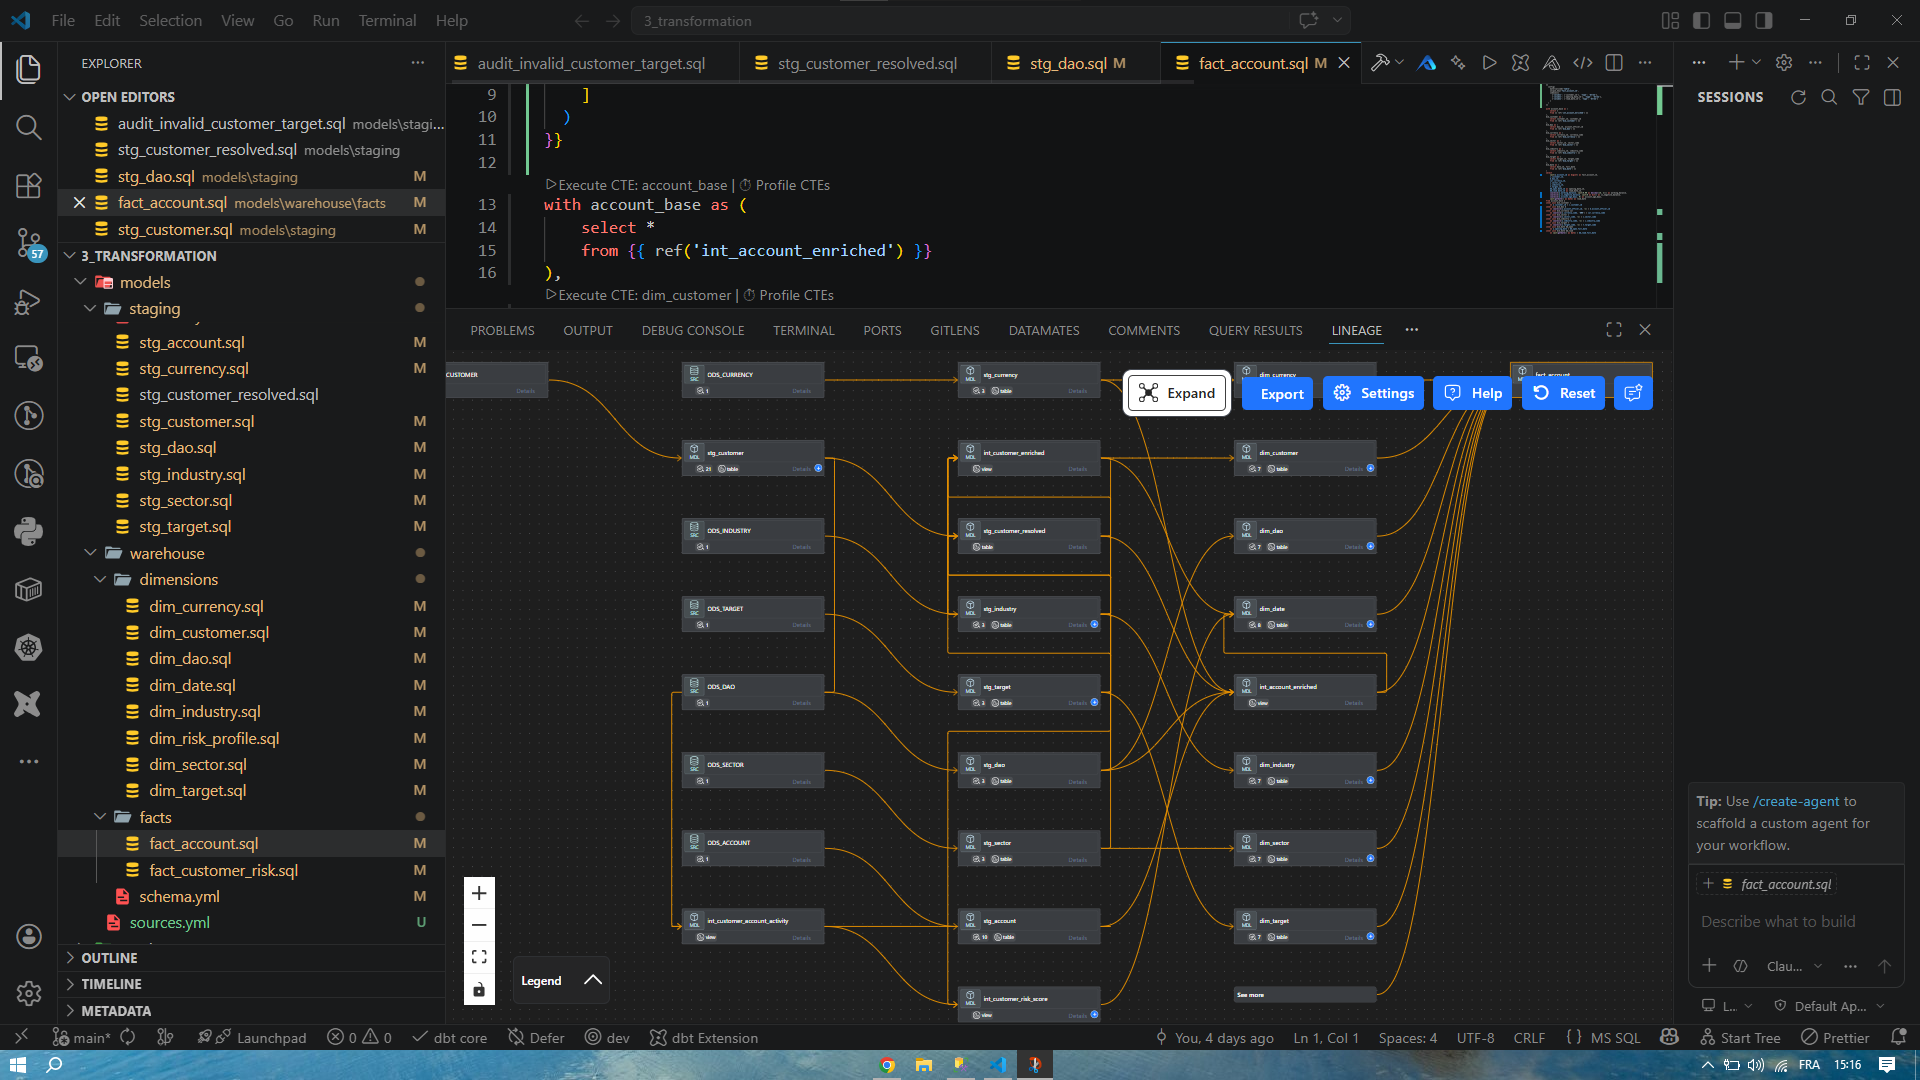
\includegraphics[width=0.85\textwidth]{figures/dbt_stg_customer_sql.png}
\caption{Excerpt of \texttt{stg\_customer.sql} showing the \texttt{OUI}/\texttt{NON} \texttt{CASE} mapping}
\label{fig:stg_customer_sql}
\end{figure}
Staging models translate French source flags into typed Boolean columns that downstream
risk SQL can reuse without ad hoc string parsing.

\begin{figure}[H]
\centering
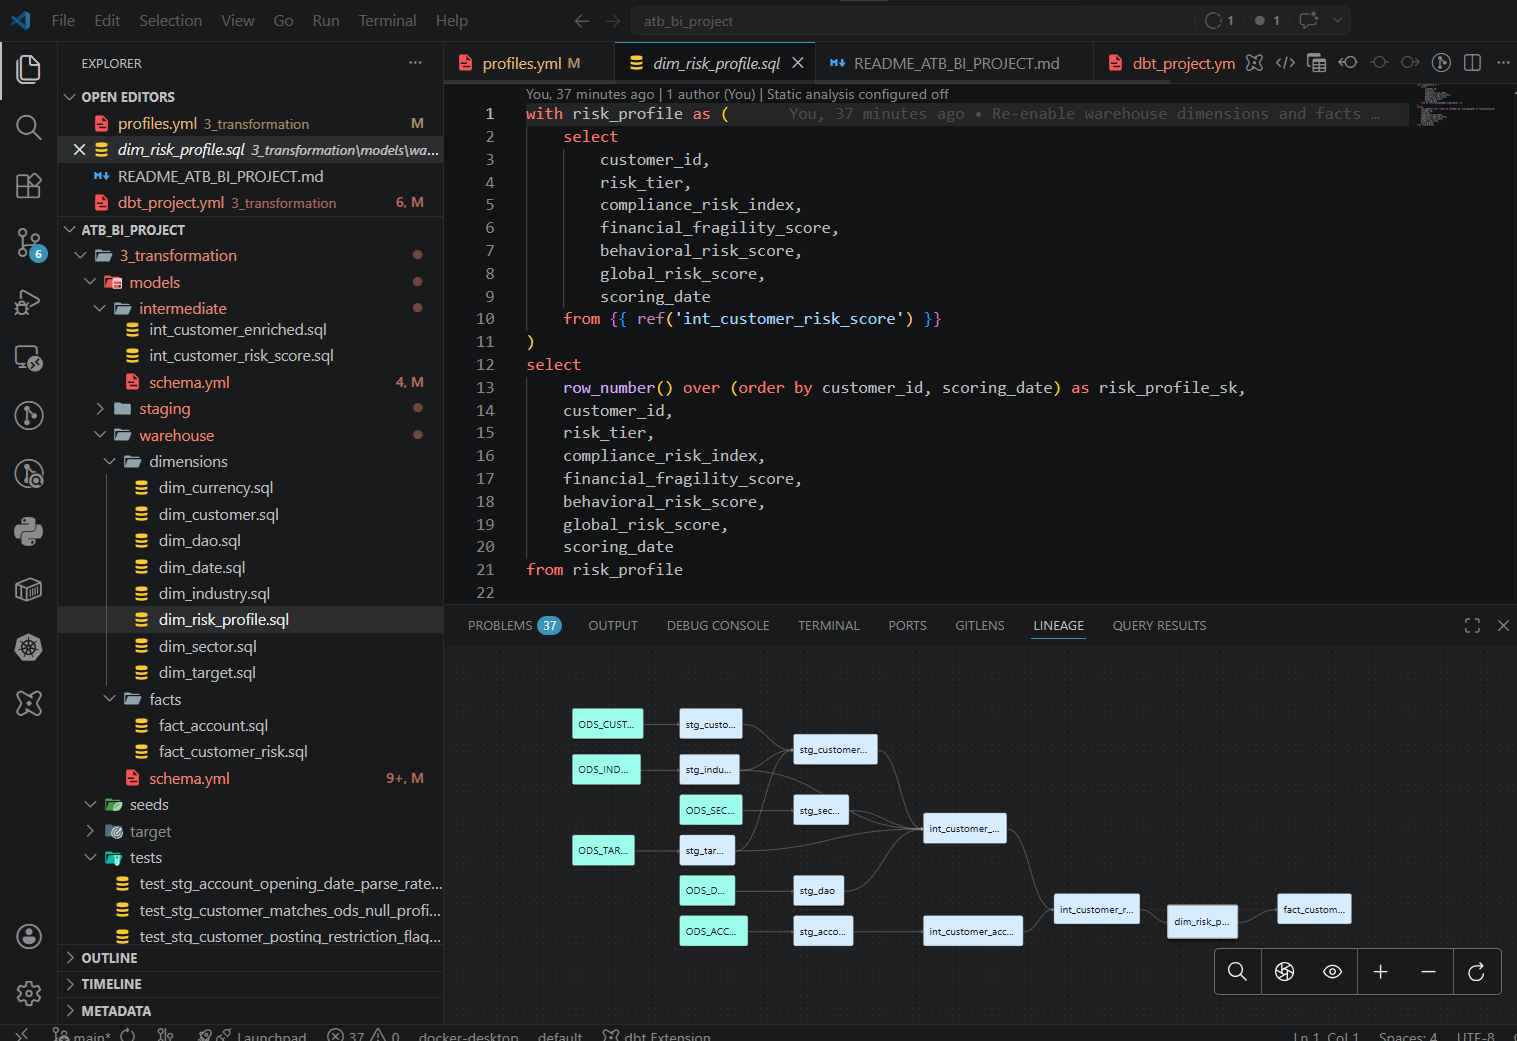
\includegraphics[width=0.85\textwidth]{figures/dbt_test_pass.png}
\caption{dbt test results --- \texttt{not\_null} / \texttt{unique} / \texttt{relationships} all green}
\label{fig:dbt_test_pass}
\end{figure}
Green \texttt{not\_null}, \texttt{unique} and \texttt{relationships} tests form the first
automated quality gate before intermediate risk models are built.

\begin{figure}[H]
\centering
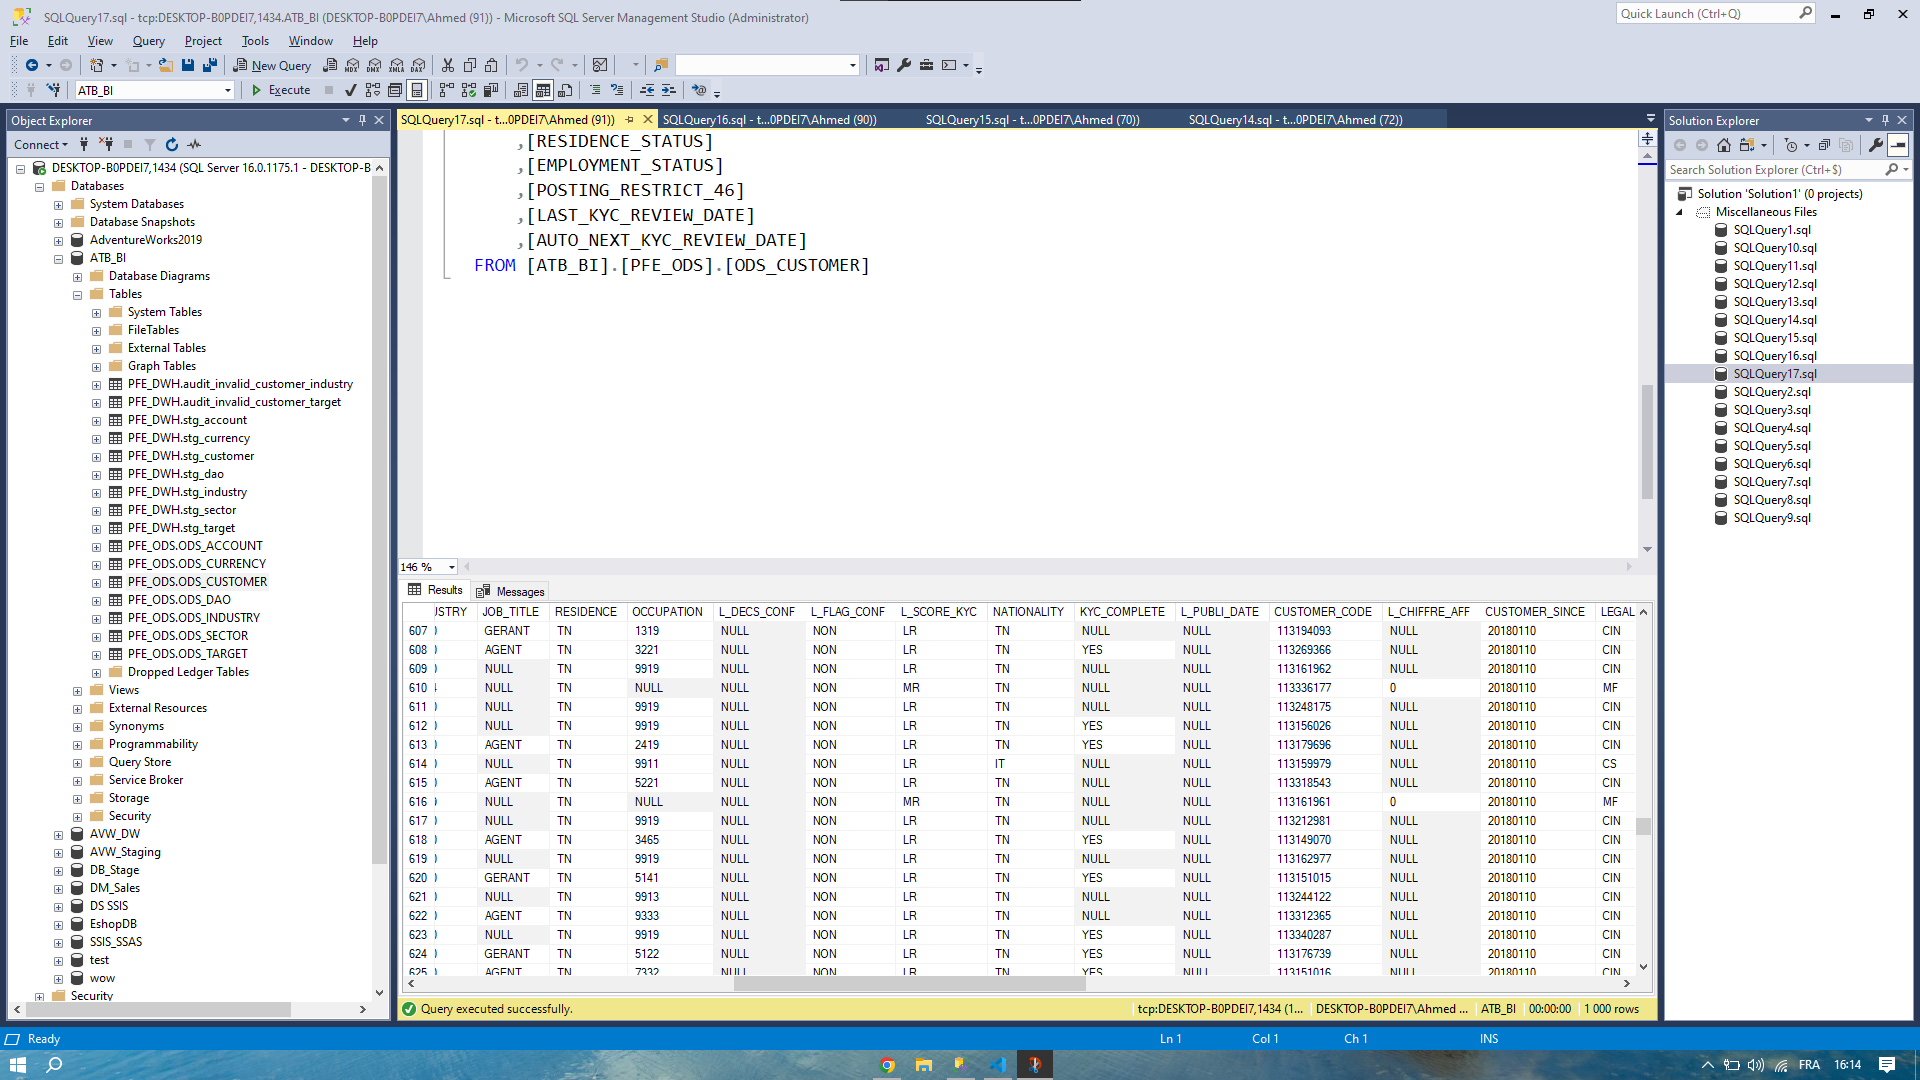
\includegraphics[width=0.85\textwidth]{figures/ods_vs_stg_compare.png}
\caption{SSMS comparison: raw \texttt{ODS\_CUSTOMER.KYC\_COMPLETE} text vs.~staged \texttt{is\_kyc\_complete} bit}
\label{fig:ods_vs_stg_compare}
\end{figure}
Side-by-side SSMS screenshots illustrate the cleaning contract: raw text codes become
consistent bit flags in staging.

\paragraph{Transform phase --- Intermediate (business logic).}
Views in \texttt{PFE\_INTERMEDIATE} enrich profiles and compute risk:
\begin{itemize}
    \item \texttt{int\_customer\_enriched}, \texttt{int\_account\_enriched};
    \item \texttt{int\_customer\_account\_activity} --- per-customer aggregates;
    \item \texttt{int\_customer\_risk\_score} --- three-pillar engine (detailed below).
\end{itemize}

\paragraph{Load phase --- Warehouse materialisation.}
Final tables are materialised in Datawarehouse. Table~\ref{tab:dim-tables}
summarises dimension loads; facts are detailed in Layer~2.

\begin{table}[H]
\centering
\caption{Dimension tables generated by the dbt warehouse load}
\label{tab:dim-tables}
\renewcommand{\arraystretch}{1.2}
\scriptsize
\begin{tabular}{|p{3.0cm}|p{2.6cm}|p{8.2cm}|}
\hline
\rowcolor{blue!15}
\textbf{Table} & \textbf{Surrogate key} & \textbf{Main attributes} \\
\hline
\texttt{dim\_customer} & \texttt{customer\_sk} & Tenure, salary, employment, KYC/PEP/compliance flags, DAO link \\
\hline
\texttt{dim\_dao} & \texttt{dao\_sk} & Officer id, area, name (+ UNKNOWN sentinel) \\
\hline
\texttt{dim\_date} & \texttt{date\_sk} & Calendar attributes (year, month, day,\ldots) \\
\hline
\texttt{dim\_sector} & \texttt{sector\_sk} & Sector code / description \\
\hline
\texttt{dim\_industry} & \texttt{industry\_sk} & Industry code / description \\
\hline
\texttt{dim\_target} & \texttt{target\_sk} & Segment code / description \\
\hline
\texttt{dim\_currency} & \texttt{currency\_sk} & ISO code (+ \texttt{UNK}) \\
\hline
\texttt{dim\_risk\_profile} & \texttt{risk\_profile\_sk} & CRI, FFS, BRS, GRS, tier, scoring date \\
\hline
\end{tabular}
\end{table}

\paragraph{Data quality framework.}
dbt schema tests enforce \texttt{not\_null}/\texttt{unique} on surrogate keys and
\texttt{relationships} from facts to dimensions. Singular SQL tests verify grain
uniqueness and staging parse rates. Failures stop the Airflow run before a broken
dashboard refresh (NFR~5).

%----------------------------------------------------------------------
\section{Baseline Approach: The Three-Pillar Weighted Risk Score}
\label{sec:three_pillar_model}
%----------------------------------------------------------------------
Although the ultimate architectural objective includes Machine Learning for
predictive risk (Release~3), we integrated inside the ELT pipeline a robust
heuristic \textbf{Baseline} serving as reference model and as ground-truth
generator for future supervised learning.

\subsection{Implementation of Business Logic inside the ELT}
In a classical decision architecture, ELT often merely moves data. Here we
enriched it with banking business logic. The SQL model
\texttt{int\_customer\_risk\_score.sql} evaluates three fundamental dimensions and
assigns specific weights according to their critical importance in ATB risk
governance:
\begin{enumerate}
    \item \textbf{Compliance Risk Index --- CRI ($40\%$):} KYC completeness, PEP,
          flags, decisions, posting restrictions, review freshness.
    \item \textbf{Financial Fragility Score --- FFS ($35\%$):} salary, balances,
          overdraft, dependents, unemployment.
    \item \textbf{Behavioural Risk Score --- BRS ($25\%$):} tenure, overdraft
          behaviour, thin balances, stale KYC.
\end{enumerate}

Figure~\ref{fig:three_pillar_tikz} synthesises the scoring flow.

\begin{figure}[H]
\centering
\begin{tikzpicture}[
  font=\scriptsize,
  pill/.style={rectangle, rounded corners=2pt, draw=#1, fill=#1!14, thick,
               align=center, minimum width=3.4cm, minimum height=1.35cm},
  outbox/.style={rectangle, rounded corners=2pt, draw=black!70, fill=gray!12, thick,
              align=center, minimum width=3.6cm, minimum height=1.2cm},
  arr/.style={->, thick}
]
  \node[pill=teal!70!black] (cri) {\textbf{CRI (40\%)}\\KYC / PEP / flags\\$[0,100]$};
  \node[pill=blue!70!black, right=0.45cm of cri] (ffs) {\textbf{FFS (35\%)}\\Salary / balance\\$[0,100]$};
  \node[pill=violet!70!black, right=0.45cm of ffs] (brs) {\textbf{BRS (25\%)}\\Tenure / behaviour\\$[0,100]$};
  \node[outbox, below=1.1cm of ffs] (grs) {\textbf{GRS} $= 0.40\,\mathrm{CRI}+0.35\,\mathrm{FFS}+0.25\,\mathrm{BRS}$};
  \node[outbox, below=0.55cm of grs] (tier) {Tier: LOW / MEDIUM / HIGH / VERY\_HIGH};
  \draw[arr] (cri) |- (grs);
  \draw[arr] (ffs) -- (grs);
  \draw[arr] (brs) |- (grs);
  \draw[arr] (grs) -- (tier);
\end{tikzpicture}
\caption{Three-pillar composite risk scoring flow}
\label{fig:three_pillar_tikz}
\end{figure}

\subsection{Detailed Calculation of Risk Indices}
Each component score ranges from $0$ (lowest risk) to $100$ (highest risk).

\subsubsection{Compliance Risk Index (CRI)}
\begin{equation}
\label{eq:cri}
\mathrm{CRI} = \min\Bigl(100,\;
\Delta_{\mathrm{KYC}}+\Delta_{\mathrm{PEP}}+\Delta_{\mathrm{FLAG}}
+\Delta_{\mathrm{DEC}}+\Delta_{\mathrm{REST}}+\Delta_{\mathrm{DATE}}\Bigr)
\end{equation}
with point increments:
\begin{equation}
\begin{aligned}
\Delta_{\mathrm{KYC}} &= 35\cdot \mathbf{1}[\texttt{is\_kyc\_complete}=0],\\
\Delta_{\mathrm{PEP}} &= 30\cdot \mathbf{1}[\texttt{is\_pep}=1],\\
\Delta_{\mathrm{FLAG}} &= 25\cdot \mathbf{1}[\texttt{is\_compliance\_flagged}=1],\\
\Delta_{\mathrm{DEC}} &= 10\cdot \mathbf{1}[\texttt{has\_compliance\_decision}=1],\\
\Delta_{\mathrm{REST}} &= 15\cdot \mathbf{1}[\texttt{posting\_restriction\_code}\neq\emptyset],\\
\Delta_{\mathrm{DATE}} &=
\begin{cases}
15 & \text{if last KYC date is NULL},\\
10 & \text{if last KYC date }> 365\text{ days},\\
0 & \text{otherwise}.
\end{cases}
\end{aligned}
\end{equation}

\subsubsection{Financial Fragility Score (FFS)}
\begin{equation}
\label{eq:ffs}
\mathrm{FFS} = \min\Bigl(100,\;
\delta_{\mathrm{SAL}}+\delta_{\mathrm{ACC}}+\delta_{\mathrm{OD}}
+\delta_{\mathrm{DEP}}+\delta_{\mathrm{EMP}}\Bigr)
\end{equation}
\begin{equation}
\begin{aligned}
\delta_{\mathrm{SAL}} &= 25\cdot \mathbf{1}[\text{salary}\le 0 \lor \text{NULL}],\\
\delta_{\mathrm{ACC}} &= 20\cdot \mathbf{1}[\texttt{account\_count}=0],\\
\delta_{\mathrm{OD}} &=
\begin{cases}
30 & \text{if total balance}<0,\\
10 & \text{if avg balance}\in[0,500]\ \text{and total}\ge 0,\\
0 & \text{otherwise},
\end{cases}\\
\delta_{\mathrm{DEP}} &= 10\cdot \mathbf{1}[\text{dependents}\ge 4],\\
\delta_{\mathrm{EMP}} &= 20\cdot \mathbf{1}[\text{employment}\in\{\texttt{UNEMPLOYED},\texttt{SANS EMPLOI},\texttt{CHOMEUR}\}].
\end{aligned}
\end{equation}

\subsubsection{Behavioural Risk Score (BRS)}
\begin{equation}
\label{eq:brs}
\mathrm{BRS} = \min\Bigl(100,\;
\gamma_{\mathrm{TEN}}+\gamma_{\mathrm{OD}}+\gamma_{\mathrm{SINGLE}}
+\gamma_{\mathrm{LOW}}+\gamma_{\mathrm{KYC}}\Bigr)
\end{equation}
\begin{equation}
\begin{aligned}
\gamma_{\mathrm{TEN}} &= 25\cdot \mathbf{1}[\text{tenure}<365],\\
\gamma_{\mathrm{OD}} &= 25\cdot \mathbf{1}[\text{any negative-balance account}],\\
\gamma_{\mathrm{SINGLE}} &= 10\cdot \mathbf{1}[\texttt{account\_count}=1],\\
\gamma_{\mathrm{LOW}} &= 15\cdot \mathbf{1}[\text{total balance}<100 \land \texttt{account\_count}>0],\\
\gamma_{\mathrm{KYC}} &= 20\cdot \mathbf{1}[\text{KYC missing or }>730\text{ days}].
\end{aligned}
\end{equation}

\subsubsection{Global Risk Score and tier mapping}
\begin{equation}
\label{eq:grs}
\boxed{\mathrm{GRS} = 0.40\,\mathrm{CRI} + 0.35\,\mathrm{FFS} + 0.25\,\mathrm{BRS}}
\end{equation}
\begin{equation}
\label{eq:tier}
\text{Risk tier} =
\begin{cases}
\texttt{LOW} & \text{if } \mathrm{GRS} < 25,\\
\texttt{MEDIUM} & \text{if } 25 \le \mathrm{GRS} < 50,\\
\texttt{HIGH} & \text{if } 50 \le \mathrm{GRS} < 75,\\
\texttt{VERY\_HIGH} & \text{if } \mathrm{GRS} \ge 75.
\end{cases}
\end{equation}

\begin{table}[H]
\centering
\caption{Justification of the three-pillar weights}
\label{tab:scoring-weights}
\renewcommand{\arraystretch}{1.2}
\scriptsize
\begin{tabular}{|p{3.0cm}|c|p{6.5cm}|p{3.0cm}|}
\hline
\rowcolor{blue!15}
\textbf{Dimension} & \textbf{Weight} & \textbf{Justification} & \textbf{Anchor} \\
\hline
Compliance (CRI) & $40\%$ & Regulatory priority (AML/KYC/PEP) in banking supervision & FATF-aligned monitoring \\
\hline
Financial (FFS) & $35\%$ & Credit / solvency pressure from income and balances & Credit-risk practice \\
\hline
Behavioural (BRS) & $25\%$ & Early-warning relationship signals & Operational risk cues \\
\hline
\end{tabular}
\end{table}

On the production snapshot, average pillars are approximately
$\mathrm{CRI}\approx 10$, $\mathrm{FFS}\approx 34$, $\mathrm{BRS}\approx 38$, giving
$\overline{\mathrm{GRS}}\approx 25.6$. The tier mix is roughly $47.7\%$
\texttt{LOW} and $52.3\%$ \texttt{MEDIUM}, with only a handful of \texttt{HIGH}
profiles --- a realistic retail-heavy distribution.

\subsection{Sensitivity Analysis of Risk Weights}
To validate the retained configuration ($40/35/25$), a sensitivity analysis
compared four weight maps on a large customer sample
(Table~\ref{tab:weights-sensitivity}).

\begin{table}[H]
\centering
\caption{Sensitivity analysis of weighting configurations}
\label{tab:weights-sensitivity}
\renewcommand{\arraystretch}{1.2}
\scriptsize
\begin{tabular}{|p{4.0cm}|c|c|c|}
\hline
\rowcolor{blue!15}
\textbf{Configuration} & \textbf{CRI / FFS / BRS} & \textbf{Alignment with financial stress} & \textbf{Compliance/audit capture} \\
\hline
\textbf{Balanced (selected)} & $\mathbf{40/35/25}$ & $\mathbf{0.835}$ & $\mathbf{91.8\%}$ \\
\hline
Compliance-heavy & $60/20/20$ & $0.621$ & $84.5\%$ \\
\hline
Finance-heavy & $20/60/20$ & $0.784$ & $71.2\%$ \\
\hline
Behaviour-heavy & $20/20/60$ & $0.693$ & $73.4\%$ \\
\hline
\end{tabular}
\end{table}

\paragraph{Analytical interpretation.}
\begin{itemize}
    \item A finance-only weighting tracks overdrafts well but under-detects PEP/KYC
          issues.
    \item A compliance-only weighting misses fragile but formally ``clean'' customers.
    \item The balanced map offers the best compromise for ATB's dual mandate: credit
          monitoring and regulatory vigilance.
\end{itemize}

\subsection{Technical Use and Scoring Results}
The weighted Global Risk Score acts at three strategic levels:
\begin{itemize}
    \item \textbf{ELT batch mode:} scores are materialised nightly into
          \texttt{fact\_customer\_risk} and \texttt{dim\_risk\_profile}.
    \item \textbf{BI restitution:} dashboards consume pre-computed tiers for instant
          cards and charts.
    \item \textbf{Future ML target:} $\mathrm{GRS}\ge 50$ defines the high-risk label
          for Release~3 supervised models, while pillar columns themselves are
          excluded from training features to avoid leakage.
\end{itemize}

%======================================================================
\section{Feature Importance Analysis}
\label{sec:feature_importance}
%======================================================================
To identify the most determining factors of the baseline risk score, we conducted
an in-depth driver analysis. This step is essential to understand which customer
and account attributes most influence GRS  and to validate that the score
encodes the signals managers actually care about.

The analysis follows two complementary approaches:
\begin{enumerate}
    \item \textbf{Composite-feature analysis:} contribution of the engineered pillars
          (CRI, FFS, BRS) to GRS under the official weights.
    \item \textbf{Raw-driver analysis:} empirical association of operational variables
          (KYC completeness, salary, overdraft, tenure,\ldots) with elevated GRS,
          observed through warehouse studies and EDA charts.
\end{enumerate}

\subsection{Results of the Analysis}
\begin{figure}[H]
\centering
\begin{minipage}{0.48\textwidth}
  \centering
  \captionof{table}{Importance of composite pillars in GRS}
  \label{tab:feature-importance-pillars}
  \renewcommand{\arraystretch}{1.2}
  \scriptsize
  \begin{tabular}{|c|l|c|c|}
    \hline
    \textbf{Rank} & \textbf{Feature} & \textbf{Weight} & \textbf{Impact} \\
    \hline
    1 & CRI (Compliance) & $40\%$ & Critical \\
    2 & FFS (Financial) & $35\%$ & Critical \\
    3 & BRS (Behavioural) & $25\%$ & High \\
    \hline
  \end{tabular}
\end{minipage}
\hfill
\begin{minipage}{0.48\textwidth}
  \centering
  \captionof{table}{Empirical ranking of raw risk drivers}
  \label{tab:feature-importance-raw}
  \renewcommand{\arraystretch}{1.2}
  \scriptsize
  \begin{tabular}{|c|l|c|}
    \hline
    \textbf{Rank} & \textbf{Raw driver} & \textbf{Impact} \\
    \hline
    1 & KYC incompleteness & Critical \\
    2 & Missing / low salary & Critical \\
    3 & Overdraft presence & High \\
    4 & Short tenure ($<365$d) & High \\
    5 & Unemployment status & Significant \\
    6 & High dependents ($\ge 4$) & Moderate \\
    7 & Single-account profile & Moderate \\
    \hline
  \end{tabular}
\end{minipage}
\end{figure}

\subsection{Interpretation of Results}
Convergence between the two views is strong:
\begin{itemize}
    \item compliance and financial pillars dominate the formal weight map ($75\%$
          combined), matching the raw dominance of KYC and salary/overdraft signals;
    \item behavioural drivers (tenure, thin balances) remain secondary but
          non-negligible exactly the role assigned to the $25\%$ BRS weight;
    \item portfolio averages ($\mathrm{CRI}$ low, $\mathrm{FFS}$/$\mathrm{BRS}$
          moderate) explain why most customers sit near the LOW/MEDIUM frontier.
\end{itemize}

\subsection{Validation of Architectural Choices}
The driver analysis validates three major design choices:
\begin{enumerate}
    \item storing CRI, FFS and BRS separately in the warehouse (explainability);
    \item dedicating dashboard pages to KYC/PEP and overdraft analytics;
    \item applying DAO filters so branch managers act on the same drivers inside
          their perimeter.
\end{enumerate}

\subsection{Cross-Validation with Exploratory Data Analysis}
These results confirm the exploratory studies exposed on the BI Studies page and
in warehouse statistics reports:

\begin{table}[H]
\centering
\caption{Convergence between EDA observations and driver importance}
\label{tab:eda-importance-convergence}
\renewcommand{\arraystretch}{1.2}
\scriptsize
\begin{tabular}{|p{6.2cm}|p{7.5cm}|}
\hline
\rowcolor{blue!15}
\textbf{EDA / warehouse observation} & \textbf{Validation by driver analysis} \\
\hline
Average CRI $\approx 10$ (generally good KYC) & Incomplete KYC remains the sharpest compliance spike when present. \\
\hline
Average FFS $\approx 34$, BRS $\approx 38$ & Salary weakness and overdraft explain the medium-risk mass. \\
\hline
Tier mix $\approx 47.7\%$ LOW / $52.3\%$ MEDIUM & Score is not collapsed on a single tier; drivers create a realistic split. \\
\hline
Sector $\times$ area heatmaps show hot spots & Geographic + sector concentration justifies constellation joins. \\
\hline
\end{tabular}
\end{table}

\subsection{Implications for Optimisation}
\begin{enumerate}
    \item \textbf{Strategic focus:} keep investing UI and data quality effort on KYC
          and balance/salary fields ($75\%$+ of decision weight).
    \item \textbf{Threshold governance:} the scarcity of \texttt{HIGH}/\texttt{VERY\_HIGH}
          tiers may justify committee review of cut-offs in a later iteration.
    \item \textbf{ML readiness:} raw drivers identified here become candidate features
          for Release~3, while pillar scores stay out of the training matrix.
\end{enumerate}

\subsection{Synthesis}
\begin{itemize}
    \item Compliance ($40\%$) and Financial ($35\%$) pillars dominate GRS by design
          and by empirical evidence.
    \item KYC completeness, salary, overdraft and tenure are the primary actionable
          levers for managers.
    \item Behavioural signals add early-warning colour without drowning regulatory
          priority.
\end{itemize}

%----------------------------------------------------------------------
\subsection{Layer 2: Data Warehouse (SQL Server \texttt{PFE\_DWH})}
%----------------------------------------------------------------------
This layer is the \textbf{central persistence zone} of the BI architecture. It
stores the eight dimensions and two facts of the constellation modelled in
Phase~2.

\paragraph{Integrity pattern (sentinel UNKNOWN).}
Dirty operational references (missing officer, unknown currency,\ldots) are not
dropped. Each dimension contains an UNKNOWN row (surrogate $-1$ or code
\texttt{UNK}); fact loaders use \texttt{LEFT JOIN} + \texttt{COALESCE(..., -1)}.
Production validation reports \textbf{zero NULL foreign keys} across
$281{,}960$ fact rows ($145{,}284 + 136{,}676$).

\begin{table}[H]
\centering
\caption{Warehouse fact volumetry and integrity audit}
\label{tab:dwh_audit}
\renewcommand{\arraystretch}{1.2}
\scriptsize
\begin{tabular}{|p{4.0cm}|c|c|c|}
\hline
\rowcolor{blue!15}
\textbf{Table} & \textbf{Rows} & \textbf{NULL FKs} & \textbf{Grain} \\
\hline
\texttt{fact\_account} & $145{,}284$ & $0$ & 1 row / account \\
\hline
\texttt{fact\_customer\_risk} & $136{,}676$ & $0$ & 1 row / customer / scoring date \\
\hline
\textbf{Total facts} & $\mathbf{281{,}960}$ & $\mathbf{0}$ & --- \\
\hline
\end{tabular}
\end{table}

\paragraph{Connectivity.}
Streamlit and quality jobs access \texttt{PFE\_DWH} through SQLAlchemy with
connection pooling (typically five active connections), avoiding handshake storms
during concurrent dashboard use.

%----------------------------------------------------------------------
\subsection{Layer 3: Business Layer (Aggregations and Statistical Calculations)}
%----------------------------------------------------------------------
The business layer is the \textbf{analytical engine} bridging warehouse tables and
Streamlit visuals. Access is centralised in \texttt{dashboard/loaders.py}, with
functions decorated by \texttt{@st.cache\_data}. Once DataFrames are in memory,
pages compute KPIs via vectorised Pandas/SQL aggregations without redundant
round-trips.

\begin{table}[H]
\centering
\caption{Algorithmic translation of steering KPIs}
\label{tab:kpi-calculs}
\renewcommand{\arraystretch}{1.2}
\scriptsize
\begin{tabular}{|p{3.2cm}|p{5.5cm}|p{5.5cm}|}
\hline
\rowcolor{blue!15}
\textbf{Displayed KPI} & \textbf{Aggregation logic} & \textbf{Threshold / meaning} \\
\hline
High-risk customers & Count where $\mathrm{GRS}\ge 50$ & Amber/red follow-up band \\
\hline
Overdraft accounts & Count where balance $<0$ & Solvency pressure \\
\hline
Incomplete KYC & Count where \texttt{is\_kyc\_complete}=0 & Compliance backlog \\
\hline
PEP population & Count where \texttt{is\_pep}=1 & Enhanced due diligence \\
\hline
Portfolio averages & Mean of GRS / CRI / FFS / BRS & Health benchmarks \\
\hline
\end{tabular}
\end{table}

Nightly rebuild is orchestrated by Airflow DAG \texttt{atb\_master\_pipeline}
(schedule \texttt{0 2 * * *}): Airbyte sync $\rightarrow$ dbt build/test
$\rightarrow$ data-quality report ($\rightarrow$ optional weekly ML train).

%----------------------------------------------------------------------
\subsection{Layer 4: Presentation (Interactive Streamlit Interface)}
%----------------------------------------------------------------------
The front-end, developed in \textbf{Python with Streamlit}, restitutes the
intelligence generated by the data layers. Its architecture rests on three
advanced software pillars:

\begin{itemize}
    \item \textbf{Dynamic routing and security (RBAC):} after authentication, the
          interface adapts to \texttt{DG\_CENTRAL}, \texttt{CHEF\_CONFORMITE},
          \texttt{CHEF\_AGENCE}, \texttt{ANALYSTE\_RISQUE} or \texttt{AUDIT}
          (read-only). Branch Managers receive DAO-scoped SQL automatically.
    \item \textbf{Design system:} reusable KPI cards, Plotly theme harmonisation,
          bilingual labels (FR/EN), and consistent risk colours.
    \item \textbf{Session state:} \texttt{st.session\_state} preserves filters and
          navigation context without useless database reloads.
\end{itemize}

\begin{figure}[H]
\centering
\begin{tikzpicture}[
  font=\scriptsize,
  role/.style={rectangle, rounded corners=2pt, draw=teal!70!black, fill=teal!10,
               thick, align=center, minimum width=2.5cm, minimum height=0.9cm},
  page/.style={rectangle, rounded corners=2pt, draw=blue!60, fill=blue!8,
               thick, align=center, minimum width=2.2cm, minimum height=0.7cm},
  arr/.style={->, thick, gray!70}
]
  \node[role] (dg) at (0,2.2) {DG\_CENTRAL};
  \node[role] (cc) at (0,1.0) {CHEF\_CONFORMITE};
  \node[role] (ag) at (0,-0.2) {CHEF\_AGENCE};
  \node[page] (ov) at (4.2,2.6) {Overview};
  \node[page] (st) at (6.6,2.6) {Studies};
  \node[page] (co) at (4.2,1.4) {Compliance};
  \node[page] (al) at (6.6,1.4) {Alerts};
  \node[page] (rk) at (4.2,0.2) {Risk};
  \node[page] (ac) at (6.6,0.2) {Accounts};
  \node[page] (dao) at (5.4,-1.0) {DAO (scoped)};
  \draw[arr] (dg) -- (ov);
  \draw[arr] (dg) -- (st);
  \draw[arr] (cc) -- (co);
  \draw[arr] (cc) -- (al);
  \draw[arr] (ag) -- (rk);
  \draw[arr] (ag) -- (ac);
  \draw[arr] (ag) -- (dao);
\end{tikzpicture}
\caption{Routing sketch for roles to analytical pages}
\label{fig:rbac_routing_tikz}
\end{figure}

\subsection{Interactive Dashboard: Architecture of Analytical Views}
The dashboard is a multi-page Streamlit application. Think of it as several
``rooms'' for different questions: a national overview for General Management, a
compliance room for the CCO, a risk deep-dive, account analytics, and a full
\textbf{dimensional catalog} so analysts can explore every Kimball dimension on
its own. Table~\ref{tab:vues-analytiques} summarises the Release~2 analytical
scope.

\begin{table}[H]
\centering
\caption{Architecture of analytical dashboard views (GIMSI Phase~3 presentation)}
\label{tab:vues-analytiques}
\renewcommand{\arraystretch}{1.2}
\scriptsize
\begin{tabular}{|p{3.2cm}|p{3.2cm}|p{7.4cm}|}
\hline
\rowcolor{blue!15}
\textbf{Module (file)} & \textbf{Analytical axis} & \textbf{KPIs and visualisations} \\
\hline
\texttt{overview.py} & Macro portfolio & Customers, accounts, total balance, avg GRS, high-risk \%, overdraft \%, risk pie, sector bars, drill-down CSV/PDF \\
\hline
\texttt{studies.py} & Cross-dimensional BI & KYC vs risk, salary vs GRS scatter, sector$\times$area heatmap, tenure bands, employment studies \\
\hline
\texttt{compliance.py} & Regulatory monitoring & PEP \%, KYC completion \%, flagged customers, overdue KYC queue \\
\hline
\texttt{alert\_inbox.py} & Operational follow-up & Prioritised alert count, severity mix, export pack \\
\hline
\texttt{risk.py} & Three-pillar deep dive & Mean CRI/FFS/BRS, tier mix, pillar histograms, customer fiche \\
\hline
\texttt{accounts.py} & Balance / overdraft & Total balance, overdraft rate, age bands, balance histogram \\
\hline
\texttt{comparison.py} & Side-by-side comparison & Two DAO areas or two sectors: customers, accounts, balance, avg risk, high-risk \%, overdraft \%, grouped bars \\
\hline
\texttt{dim\_customer\_page.py} & Customer dimension & See Table~\ref{tab:dim_dashboard_kpis} \\
\hline
\texttt{dim\_dao\_page.py} & Branch / DAO network & Branch count, areas, balance \& overdraft by area, risk scatter \\
\hline
\texttt{dim\_sector\_page.py} & Economic sectors & Top sector by accounts, highest avg risk, max overdraft \% \\
\hline
\texttt{dim\_industry\_page.py} & Industries & Industry volume, risk bubble, account exposure \\
\hline
\texttt{dim\_target\_page.py} & Segments & Largest segment, highest-risk segment, top balance segment \\
\hline
\texttt{dim\_currency\_page.py} & FX reference & Currency count, exposure, overdraft \& risk by currency \\
\hline
\texttt{dim\_date\_page.py} & Calendar / vintage & Days covered, openings by year, balance by vintage \\
\hline
\end{tabular}
\end{table}

%----------------------------------------------------------------------
\subsubsection*{Executive, risk and compliance pages}
%----------------------------------------------------------------------
Figure~\ref{fig:dashboard_overview} is the national entry point. In everyday
language: the top cards answer ``how big is the book and how healthy is it?'',
while the charts answer ``where does the risk sit?''. The page articulates four
zones:
\begin{enumerate}
    \item \textbf{Navigation sidebar:} BI groups, language toggle, AI explanation
          controls;
    \item \textbf{System status / freshness:} last warehouse load timestamp;
    \item \textbf{Global KPIs:} customers, accounts, balances, average risk,
          high-risk share, overdraft share;
    \item \textbf{Analytical charts:} risk-tier composition, three-pillar averages
          by tier, currency treemap and top sectors by balance, with CSV/PDF export.
\end{enumerate}

\begin{figure}[H]
\centering
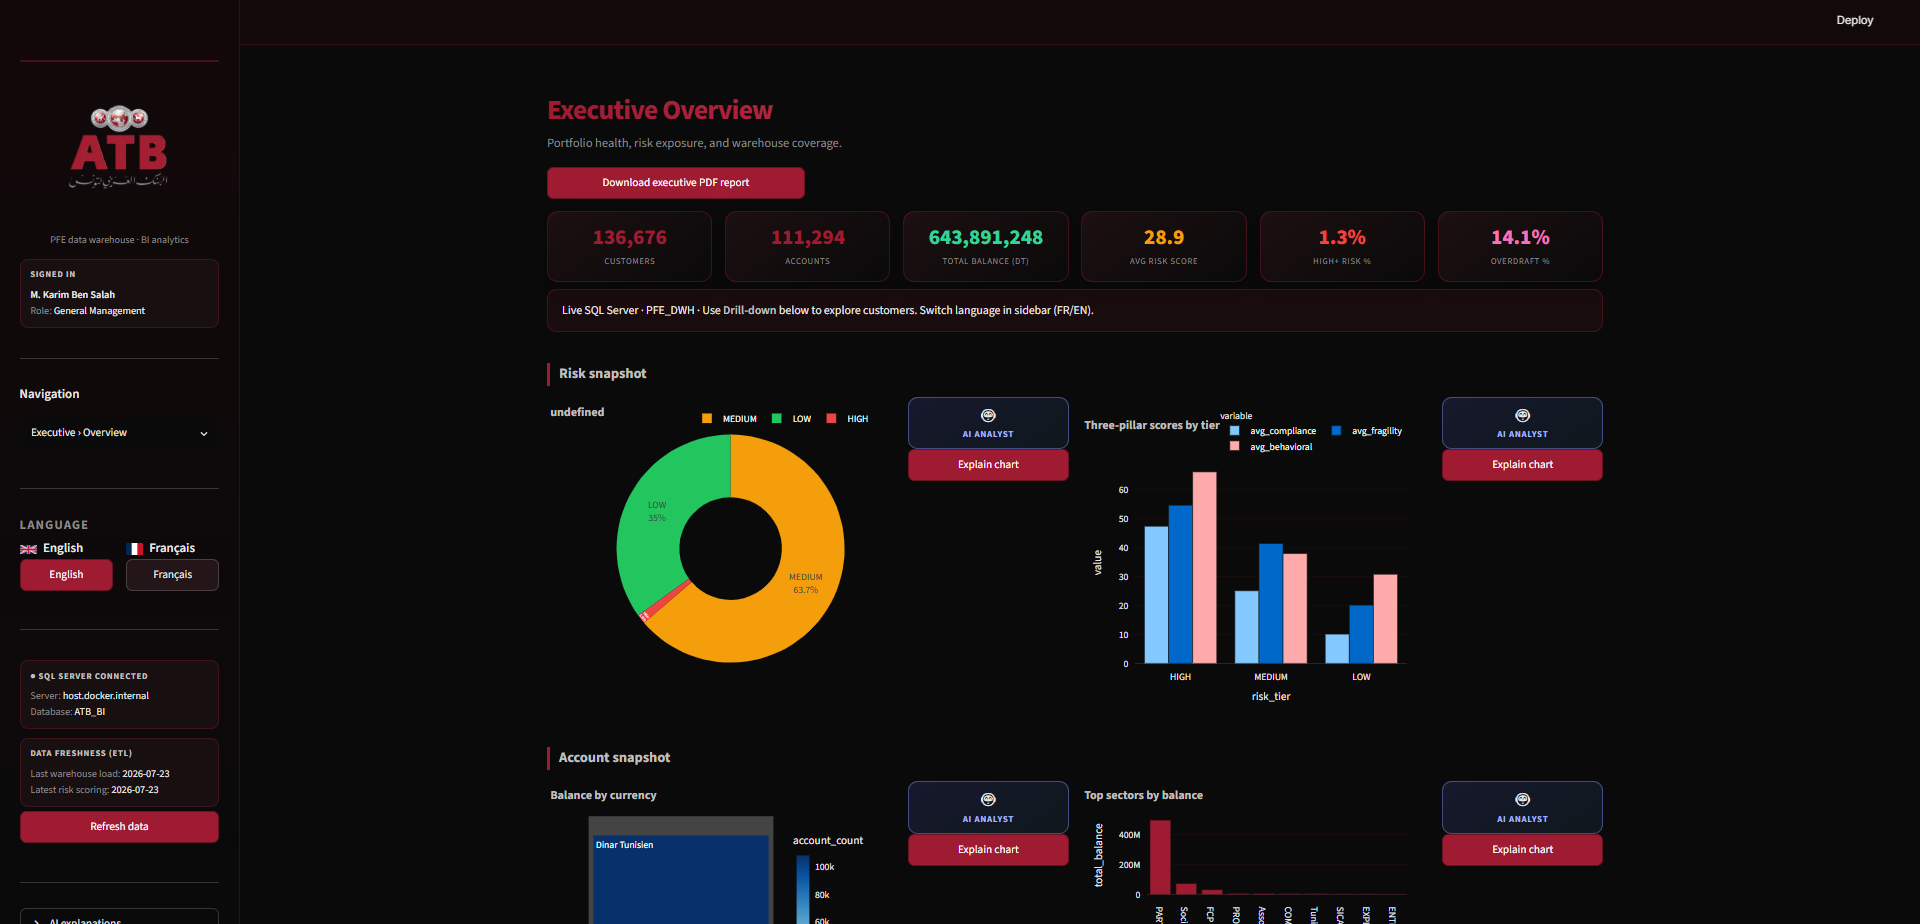
\includegraphics[width=0.88\textwidth]{figures/dash_overview_kpis.png}
\caption{Executive Overview portfolio KPIs, risk distribution and sector exposure}
\label{fig:dashboard_overview}
\end{figure}
\noindent Six headline cards (136{,}676 customers, 111{,}294 accounts,
643~M~DT balance, avg GRS 28.9, 1.3\% high-risk, 14.1\% overdraft) sit above a
risk-tier donut, three-pillar bars by tier, a currency treemap and top sectors
by balance. The sidebar confirms SQL Server connectivity and warehouse freshness.

\begin{figure}[H]
\centering
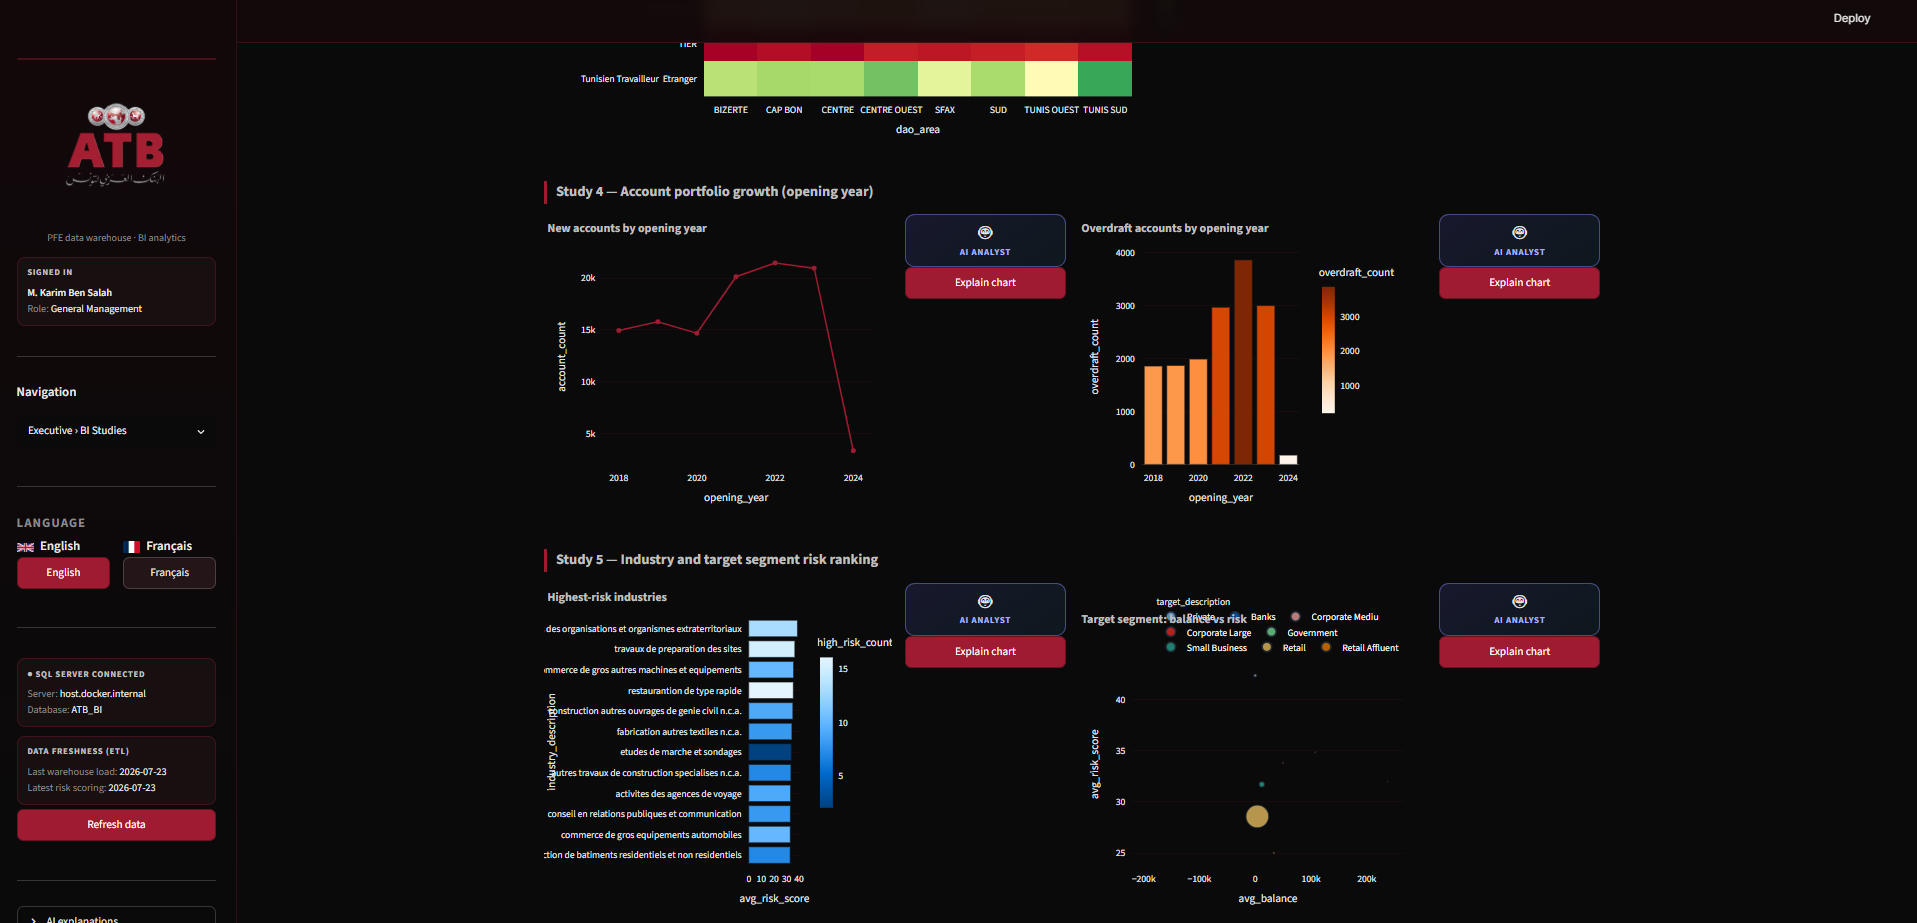
\includegraphics[width=0.88\textwidth]{figures/dash_studies.png}
\caption{BI Studies page account openings by vintage and industry, segment, risk}
\label{fig:dash_studies}
\end{figure}
\noindent Study panels deepen the overview: new and overdraft
accounts by opening year show portfolio growth, while highest-risk industries
and a balance-vs-risk scatter by target segment highlight concentration pockets
for committee follow-up.

\begin{figure}[H]
\centering
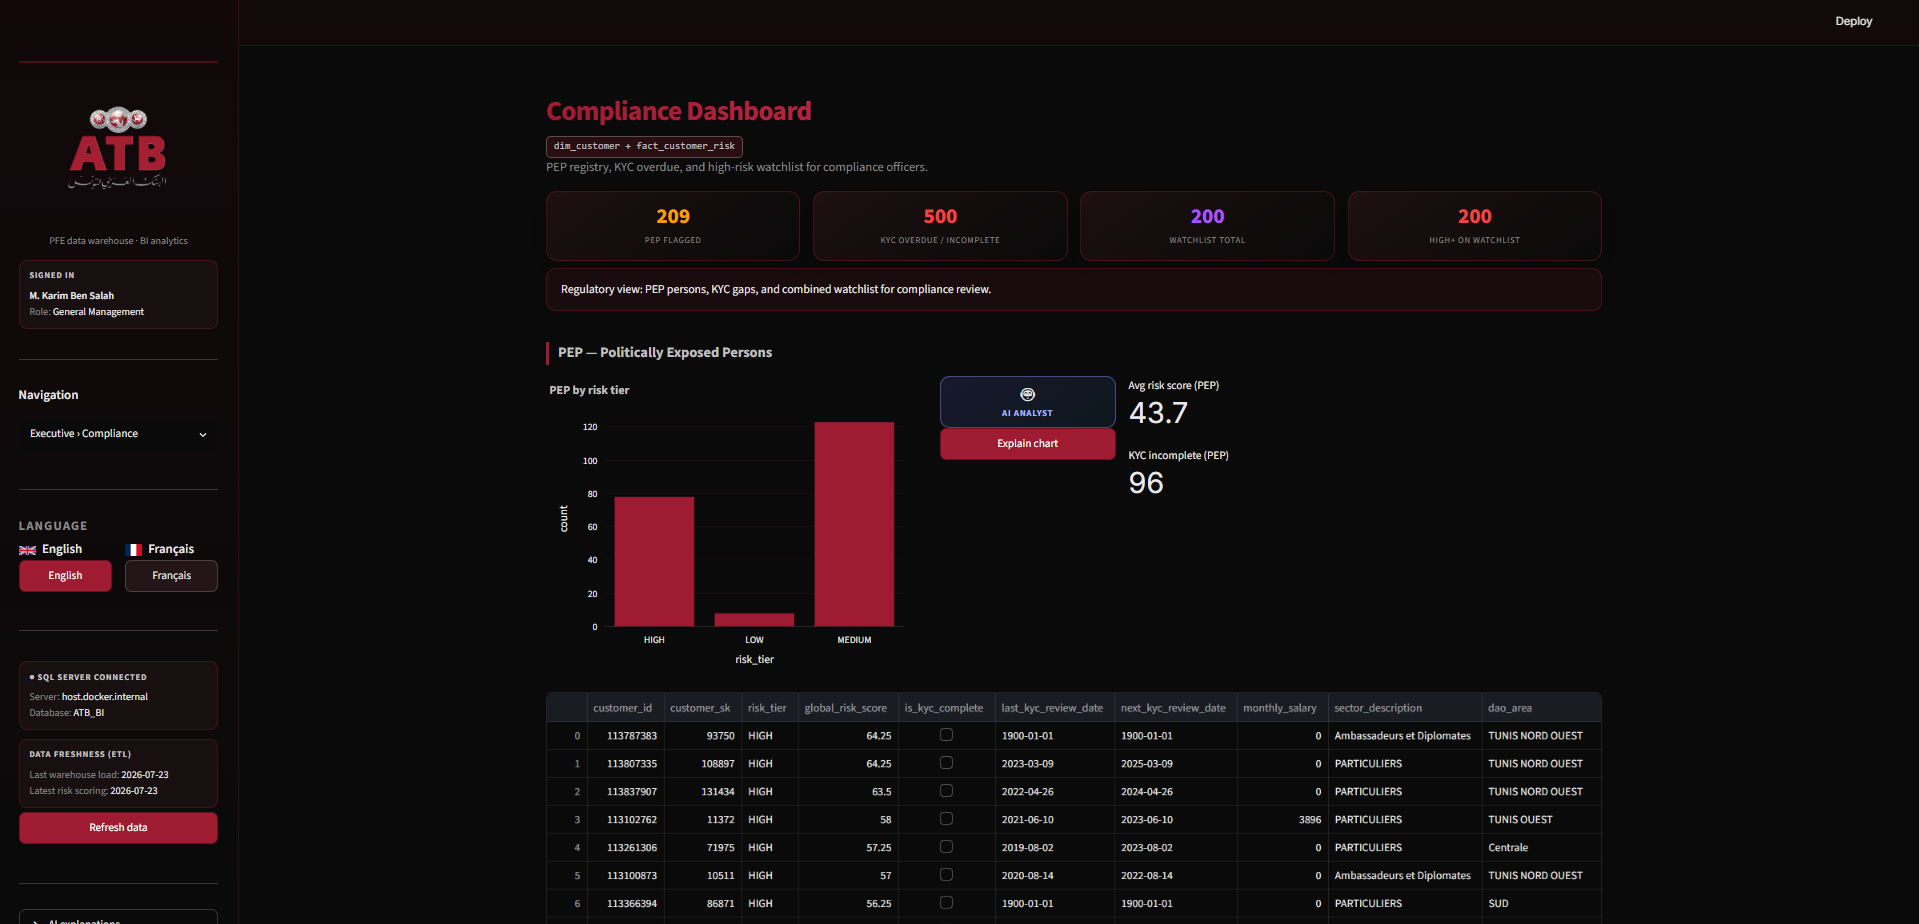
\includegraphics[width=0.88\textwidth]{figures/dash_compliance.png}
\caption{Compliance Dashboard --- PEP registry, KYC overdue and high-risk watchlist}
\label{fig:dash_compliance}
\end{figure}
\noindent Compliance officers see PEP flagged (209), KYC overdue
(500) and watchlist totals at a glance, with PEP-by-tier bars and a row-level
customer table joining \texttt{Dimension customer} to \texttt{fact customer risk}
for enhanced due diligence.

\begin{figure}[H]
\centering
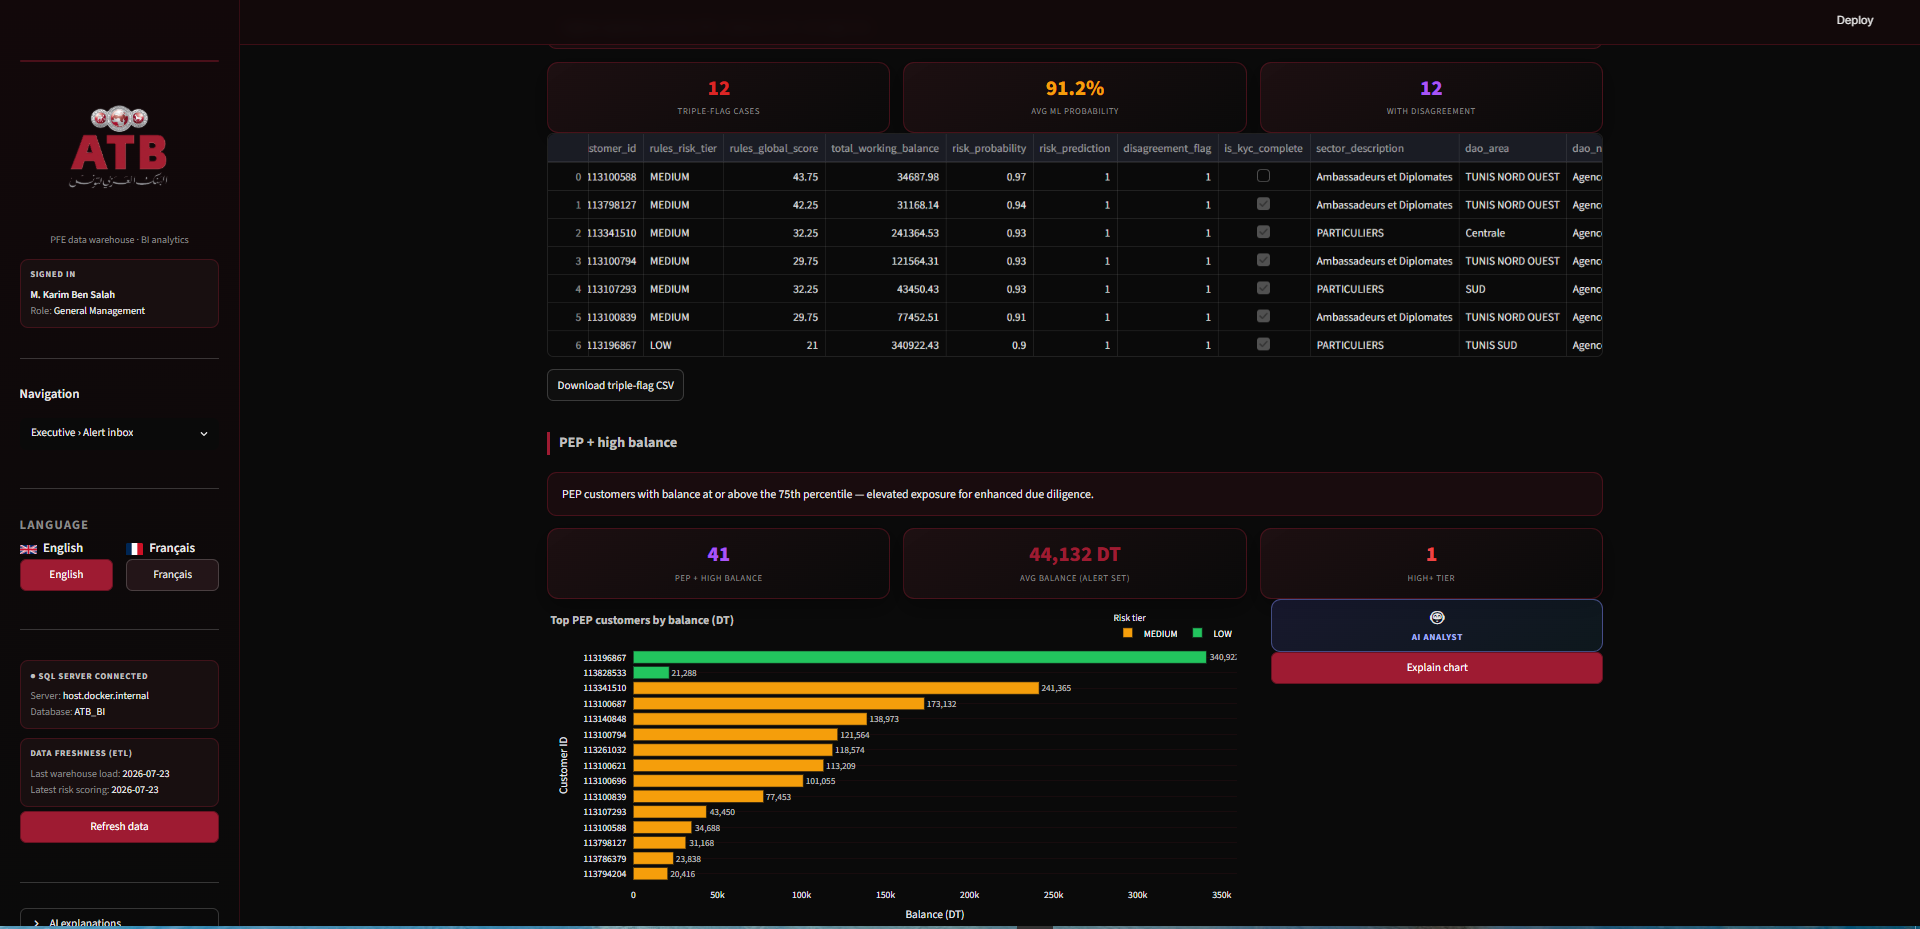
\includegraphics[width=0.88\textwidth]{figures/dash_alert_inbox.png}
\caption{Alert inbox triple-flag cases, ML disagreement and PEP high-balance}
\label{fig:dash_alert_inbox}
\end{figure}
\noindent The inbox prioritises cases where rules, KYC and ML
signals coincide (triple-flag), surfaces ML/rules disagreements for review, and
lists PEP customers with balances above the 75th percentile ready for CSV
export to the compliance team.

\begin{figure}[H]
\centering
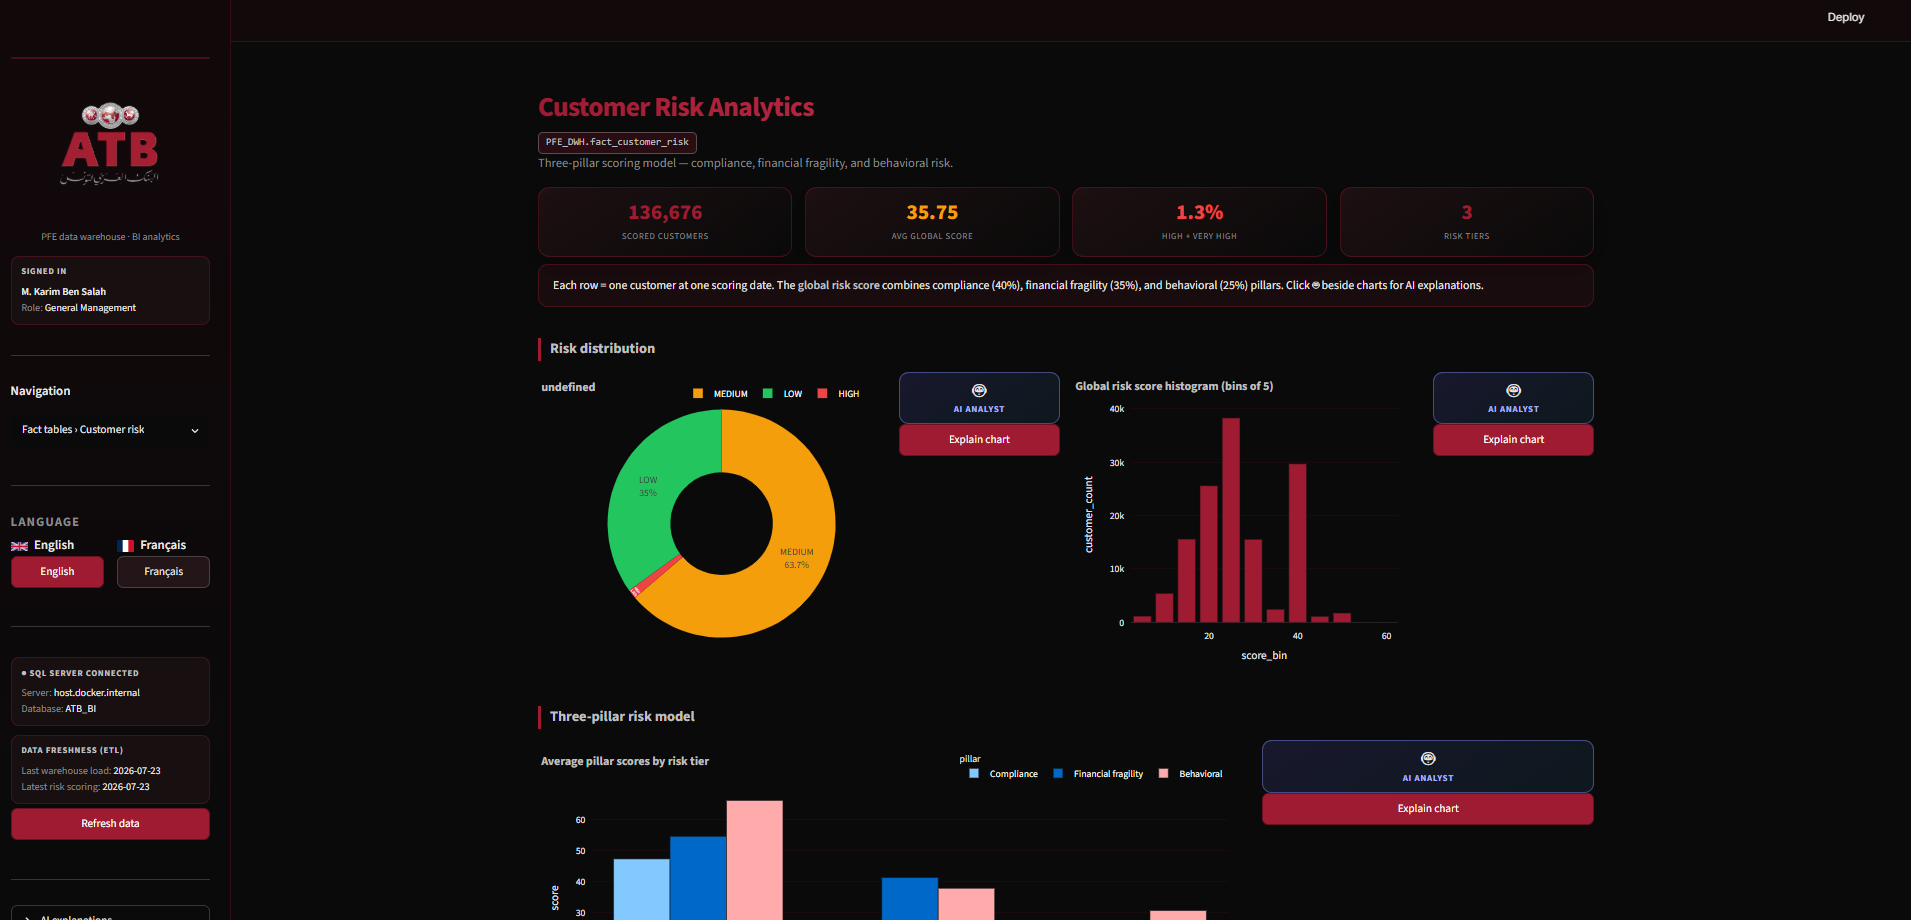
\includegraphics[width=0.88\textwidth]{figures/dash_risk_pillars.png}
\caption{Customer Risk Analytics GRS distribution and three-pillar breakdown}
\label{fig:dash_risk_pillars}
\end{figure}
\noindent Built on the 40/35/25 weighting (compliance /
financial fragility / behavioural), the page shows tier mix (1.3\% high), the
GRS histogram and average pillar scores by tier explaining \emph{why} a
customer lands in HIGH rather than only showing the final score.

\begin{figure}[H]
\centering
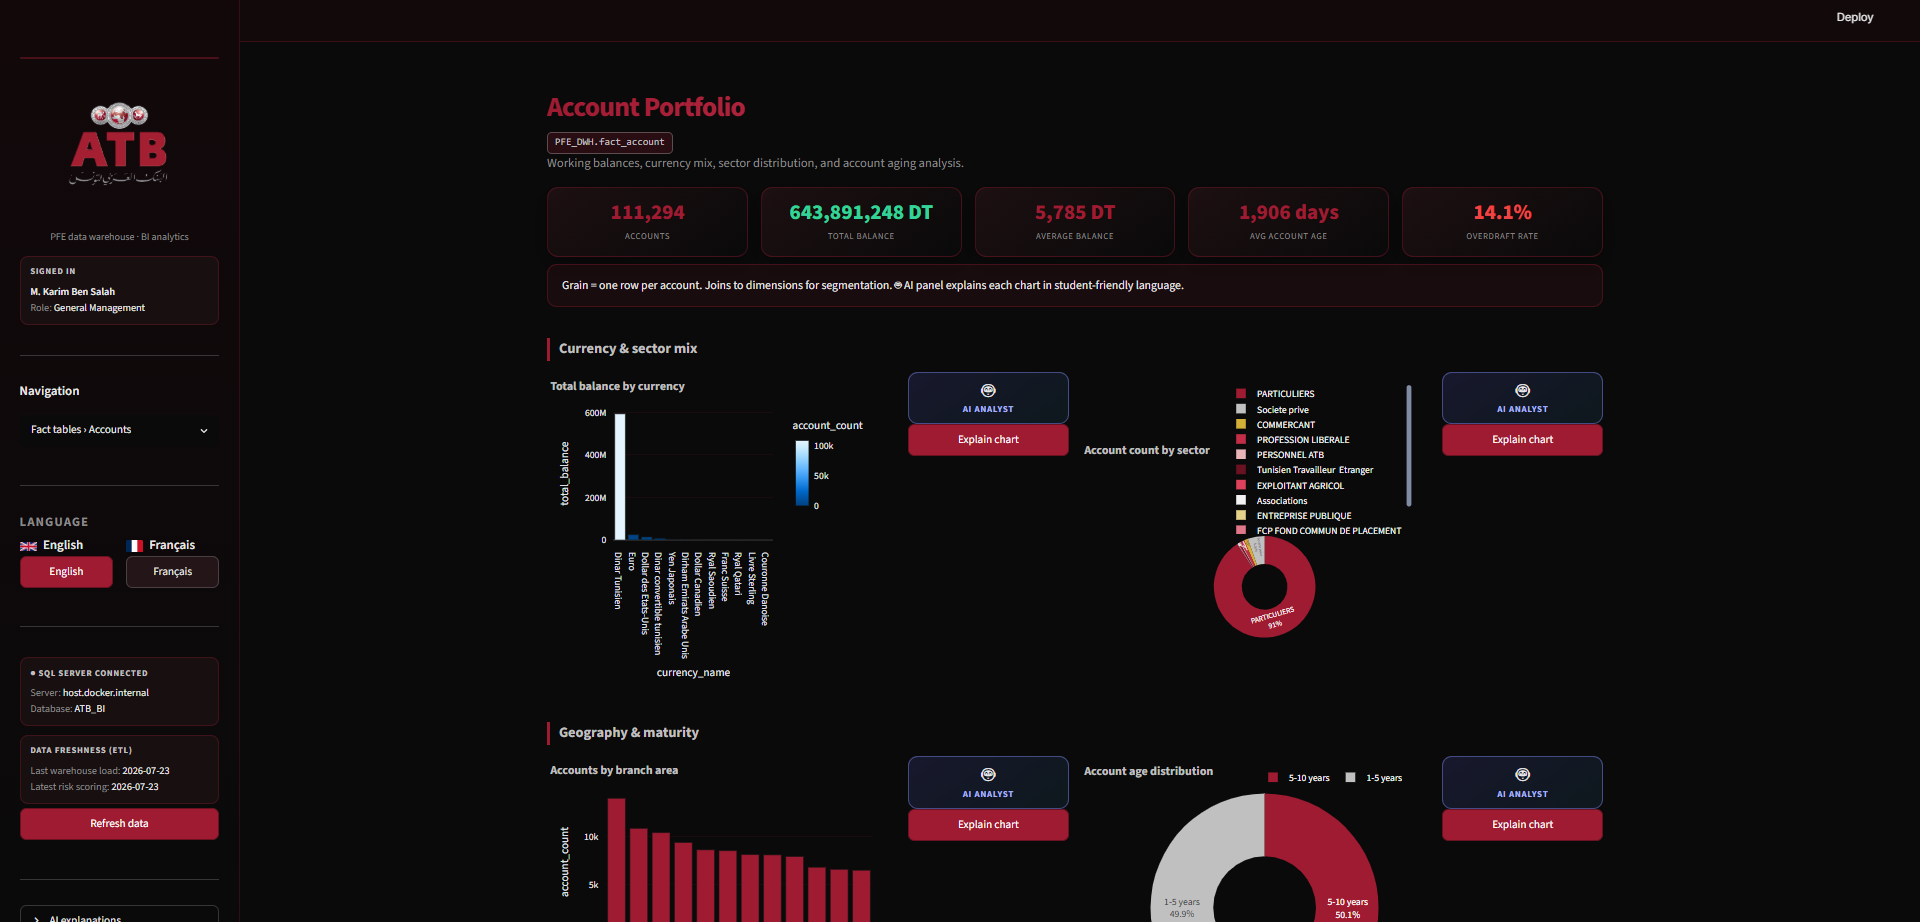
\includegraphics[width=0.88\textwidth]{figures/dash_accounts.png}
\caption{Account Portfolio balances, currency mix and sectors}
\label{fig:dash_accounts}
\end{figure}
\noindent Grain is one row per account from
\texttt{fact\_account}: KPIs cover volume, total/average balance, age and
overdraft rate; charts break exposure by currency and sector, then geography
and account-age bands.

\paragraph{DAO / sector comparison (US~13).}
Beyond single-dimension pages, the dashboard exposes a dedicated
\textbf{Comparison} view so Central General Management
and risk analysts can confront two entities side by side. The user selects the
comparison mode \emph{DAO area} or \emph{sector} then picks Entity~A and
Entity~B. The page returns a metric table (customers, accounts, total balance,
average GRS, high-risk share, overdraft rate) with deltas, a grouped bar chart,
and complementary customer-mix / average-risk visuals. This answers US~13
directly: mathematical comparison of risk levels by geographic zone or by
economic sector without exporting data to Excel.

% --- SCREENSHOT PLACEHOLDER: Save your screenshot as report/figures/Comparisim_mode.png and uncomment below:
%\begin{figure}[H]
%\centering
%\includegraphics[width=0.55\textwidth]{figures/Comparisim_mode.png}
%\caption{Streamlit Comparison page side-by-side sectors: metric deltas and grouped bars}
%\label{fig:dash_comparison_dao}
%\end{figure}
\noindent Figure~\ref{fig:dash_comparison_dao} will show the live
Comparison screen once the screenshot is inserted: two DAO areas selected in
the header, the delta table in the centre, and the Plotly grouped bars below the same panel also supports an optional Gemini ``Explain chart'' call.

\paragraph{AI-generated chart explanations.}
Selected Plotly charts expose an ``Explain chart'' panel powered by Google Gemini. On API failure, a deterministic template fallback
still returns a usable sentenceso FR~6 stays available even offline.
\begin{figure}[H]
\centering
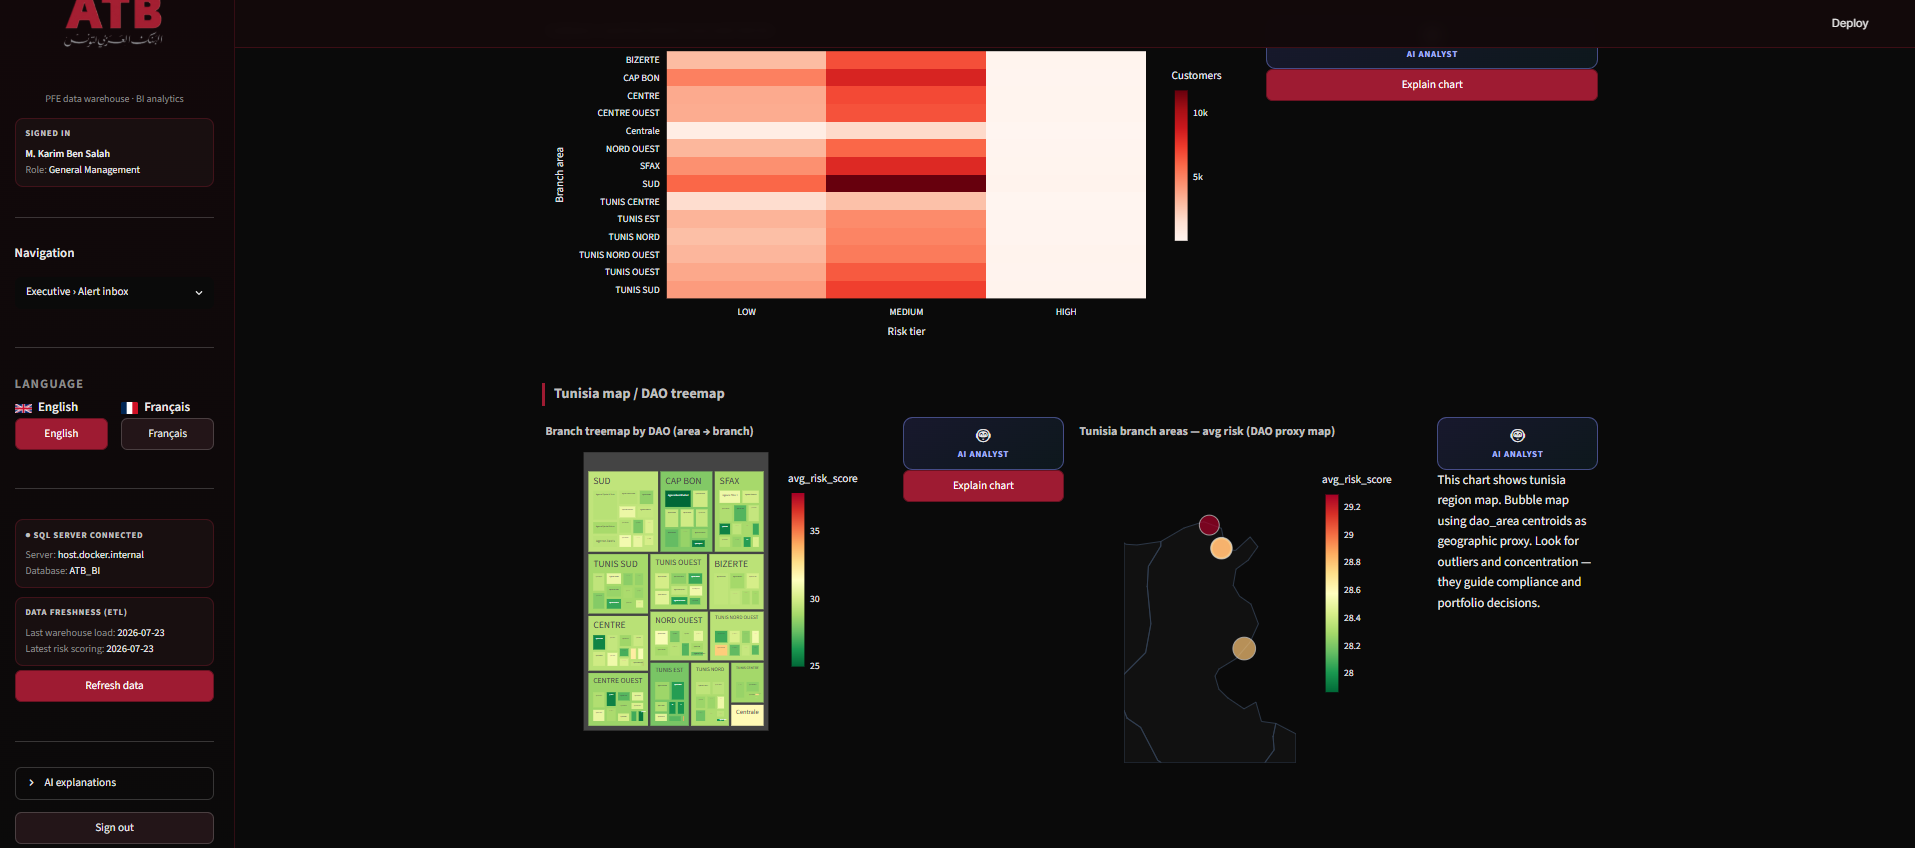
\includegraphics[width=0.85\textwidth]{figures/dash_ai_explain.png}
\caption{Gemini AI explanation panel beside a Plotly chart}
\label{fig:dash_ai_explain}
\end{figure}
\noindent Each chart can request a plain-language interpretation
calibrated to the user's role; the panel appears beside the visualisation so
managers never leave the analytical context.

%----------------------------------------------------------------------
\subsubsection*{Dimension dashboards (Kimball catalog in Streamlit)}
%----------------------------------------------------------------------
A constellation warehouse is only half useful if managers only ever see facts.
Release~2 therefore exposes \textbf{one Streamlit page per major dimension}.
Each page joins the dimension to \texttt{fact account} and/or
\texttt{fact customer risk}, so a ``dimension view'' is never a static
dictionary it is an analytical lens.

\begin{table}[H]
\centering
\caption{Dimension dashboard KPIs and charts implemented in Streamlit}
\label{tab:dim_dashboard_kpis}
\renewcommand{\arraystretch}{1.2}
\scriptsize
\begin{tabular}{|p{2.8cm}|p{5.0cm}|p{6.4cm}|}
\hline
\rowcolor{blue!15}
\textbf{Dimension page} & \textbf{Header KPIs} & \textbf{Main charts / tables} \\
\hline
\textbf{Customers} & Total customers; avg salary (DT); avg tenure (days); KYC complete \%; PEP \%; compliance-flagged \% & Gender pie; employment bars; compliance flag pie; KYC$\times$tier bars; salary bands; tenure bands; marital pie; sector bars; residence \\
\hline
\textbf{DAO / Branches} & Branch (DAO) count; area count; department count; top area by balance & Area treemap; branch counts; balance by area; overdraft by area; risk vs volume scatter; branch directory \\
\hline
\textbf{Sectors} & Sector count; top sector by accounts; highest avg risk; max overdraft \% & Catalog bars; risk ranking; balance by sector; overdraft rate; accounts$\times$risk bubble; high-risk counts \\
\hline
\textbf{Industries} & Industry count; top industries by customers/accounts; risk focus & Concentration bars; account exposure; risk-vs-volume bubble \\
\hline
\textbf{Target segments} & Segment count; largest segment; highest-risk segment; top balance segment & Segment mix pie; avg risk by segment; balance \& accounts by segment; balance-vs-risk scatter \\
\hline
\textbf{Currencies} & Currency count; exposure totals; overdraft focus & Reference table; account exposure; overdraft \& risk by FX; balance treemap \\
\hline
\textbf{Calendar} & Calendar days; years covered; min/max year & Dates per year; weekend split; month/quarter seasonality; openings by year; balance by vintage \\
\hline
\end{tabular}
\end{table}

These dimension pages matter for three concrete reasons:
\begin{itemize}
    \item \textbf{Traceability:} a committee can open \texttt{dim\_sector} and see
          exactly which economic activities concentrate overdraft or high GRS;
    \item \textbf{Branch governance:} \texttt{dim\_dao} is the geographic cockpit
          behind US~06 the same page becomes DAO-scoped for a Branch Manager;
    \item \textbf{Feature discovery for Release~3:} salary bands, tenure bands and
          KYC flags visible here are the raw drivers later reused by ML features.
\end{itemize}

\begin{figure}[H]
\centering
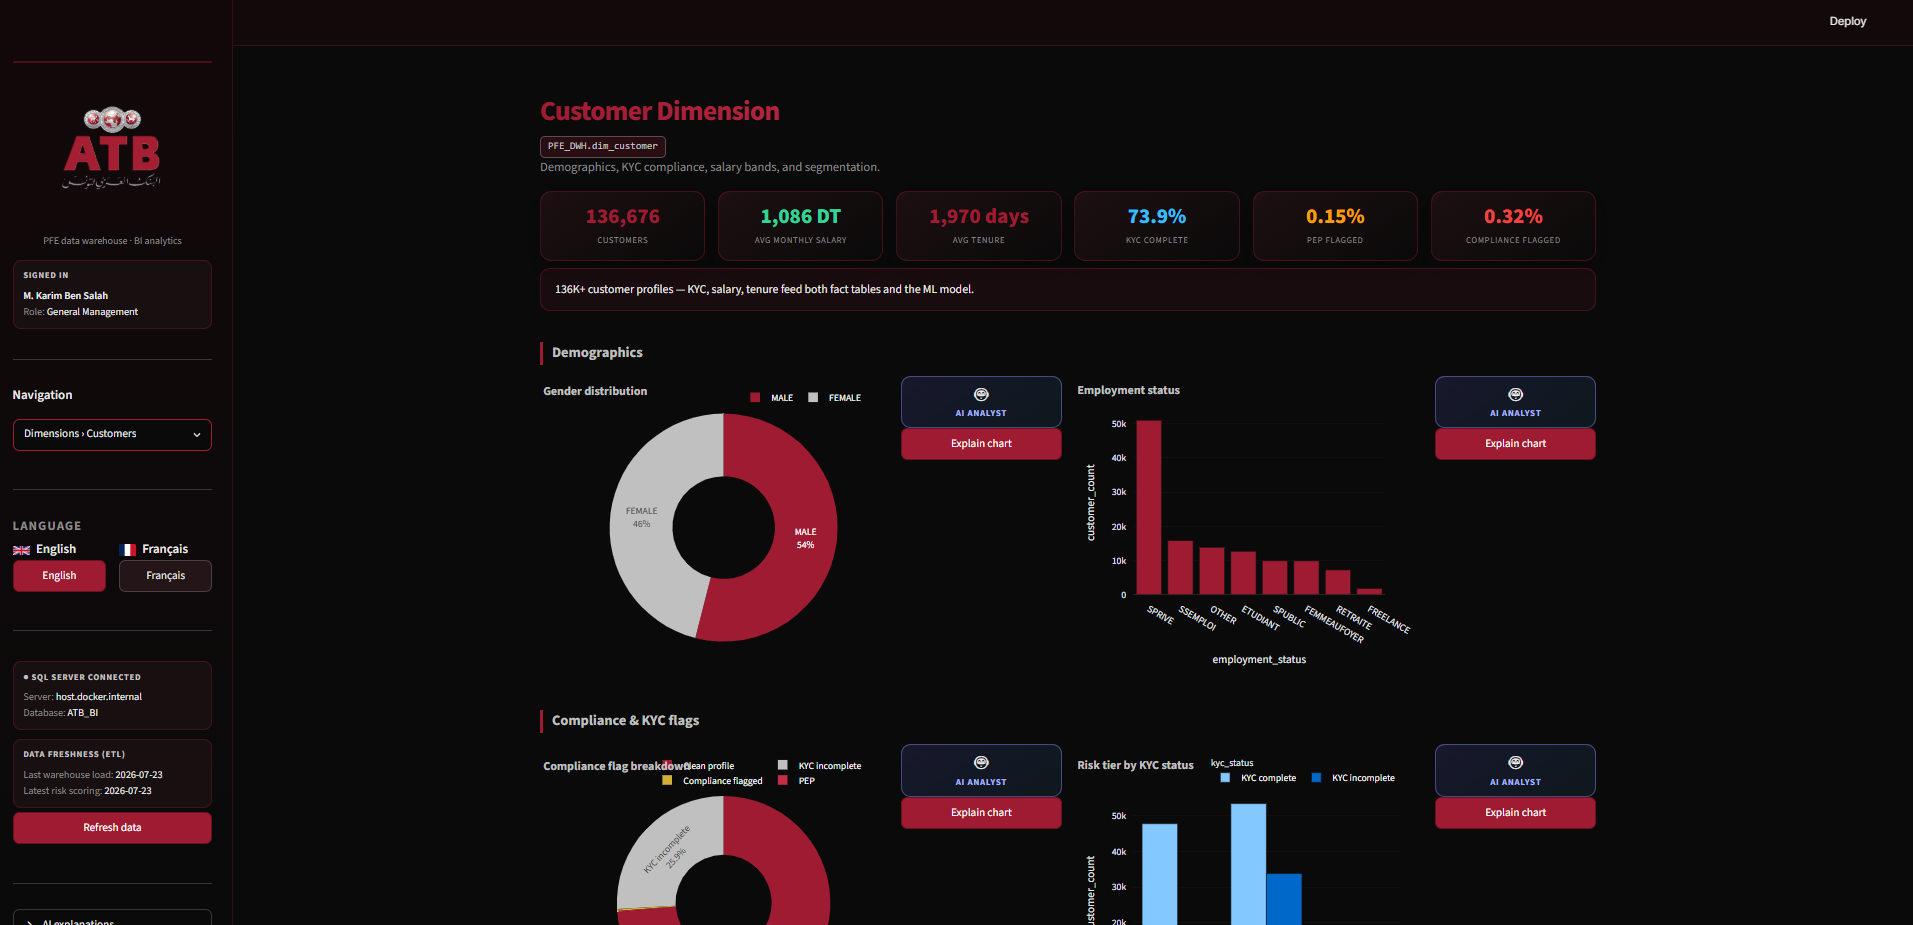
\includegraphics[width=0.88\textwidth]{figures/dash_dim_customer.png}
\caption{Customer dimension demographics, KYC compliance and salary context}
\label{fig:dash_dim_customer}
\end{figure}
\noindent Header KPIs summarise book size, salary, tenure and
regulatory flags (KYC 73.9\%, PEP 0.15\%). Gender and employment charts feed
both commercial steering and the demographic features later reused by ML.

\begin{figure}[H]
\centering
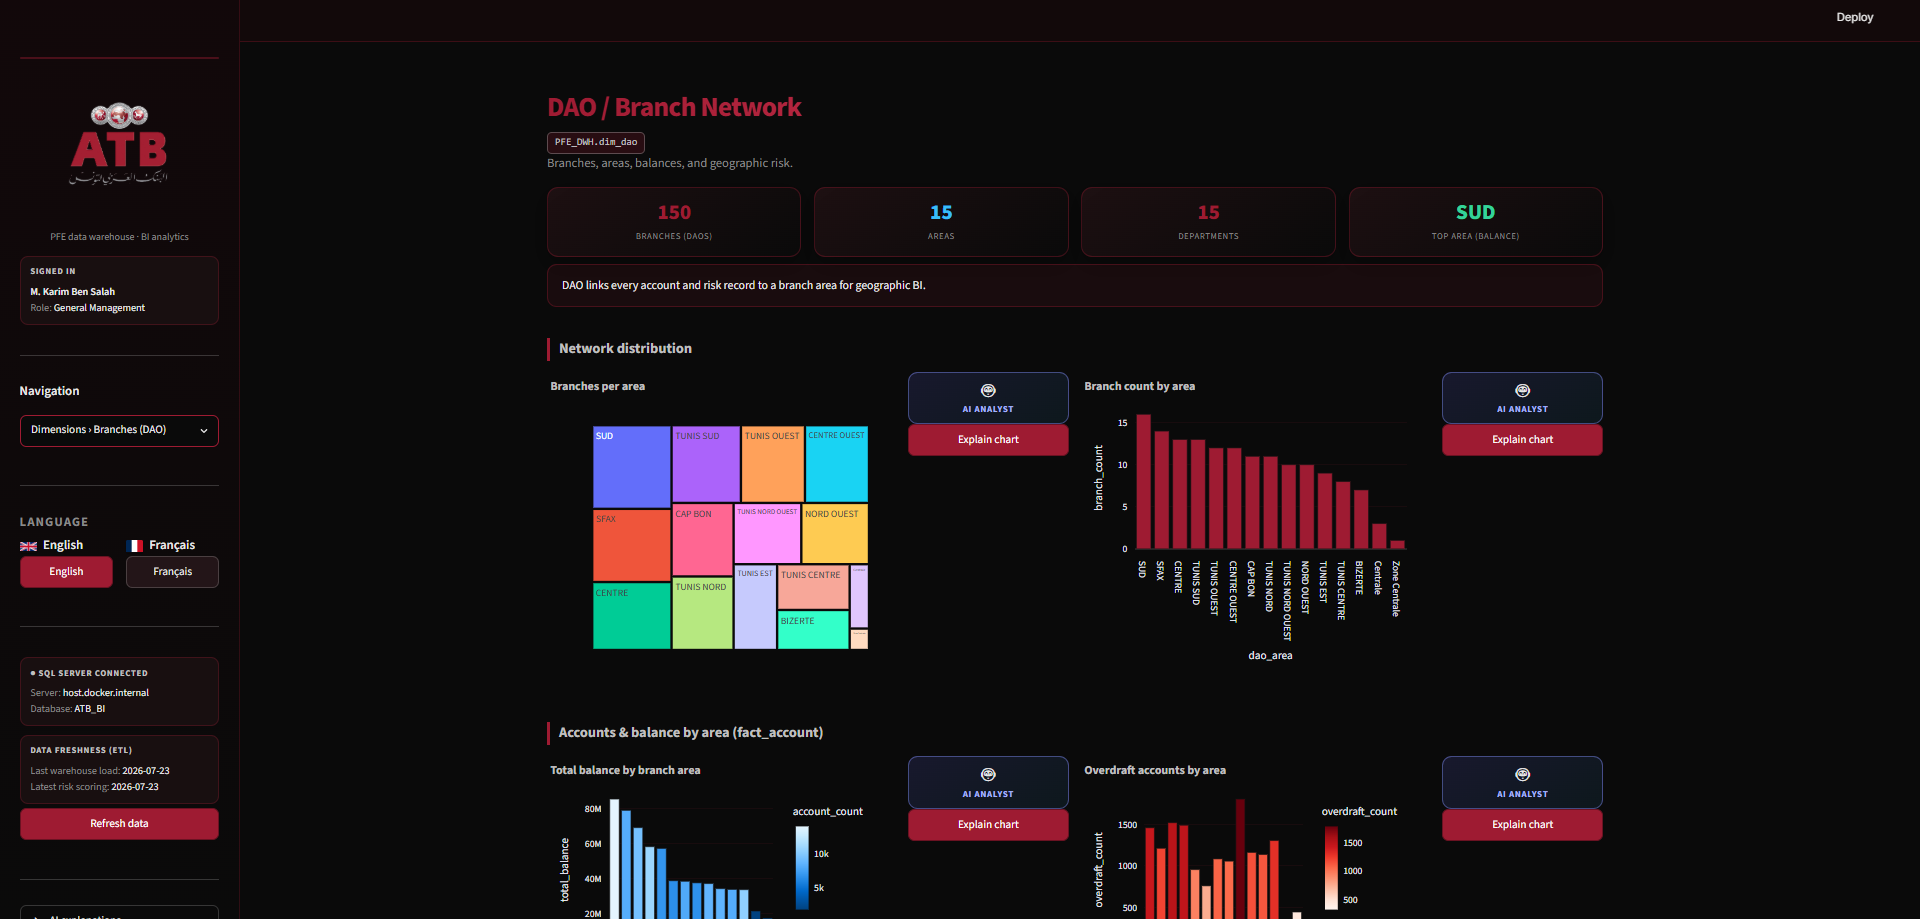
\includegraphics[width=0.88\textwidth]{figures/dash_dim_dao.png}
\caption{DAO / Branch Network area treemap, balance and overdraft by region}
\label{fig:dash_dim_dao}
\end{figure}
\noindent 150 DAOs across 15 areas: the treemap and branch-count
bars locate the network; balance and overdraft-by-area charts surface geographic
concentration the same page is DAO-scoped for Branch Managers (US~06).

\begin{figure}[H]
\centering
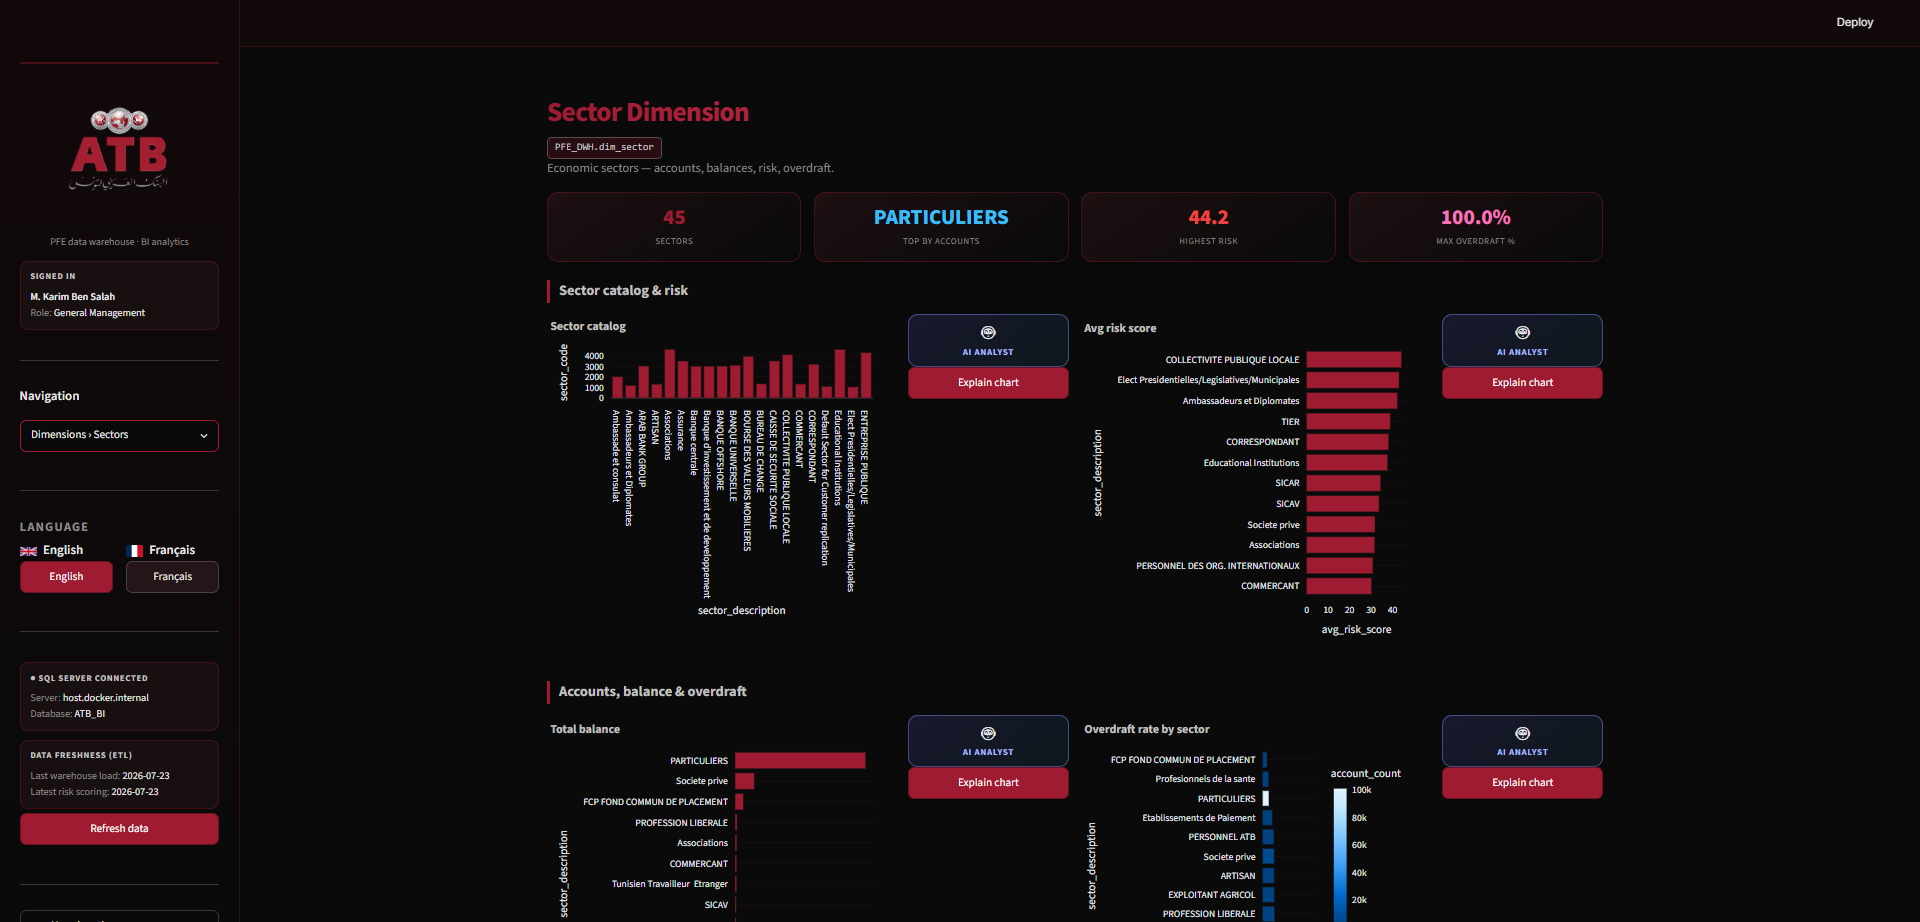
\includegraphics[width=0.88\textwidth]{figures/dash_dim_sector.png}
\caption{Sector dimension catalog, risk ranking, balance and overdraft rate}
\label{fig:dash_dim_sector}
\end{figure}
\noindent Forty-five economic sectors ranked by volume and
average risk; balance and overdraft-rate charts show which activities
concentrate solvency pressure.

\begin{figure}[H]
\centering
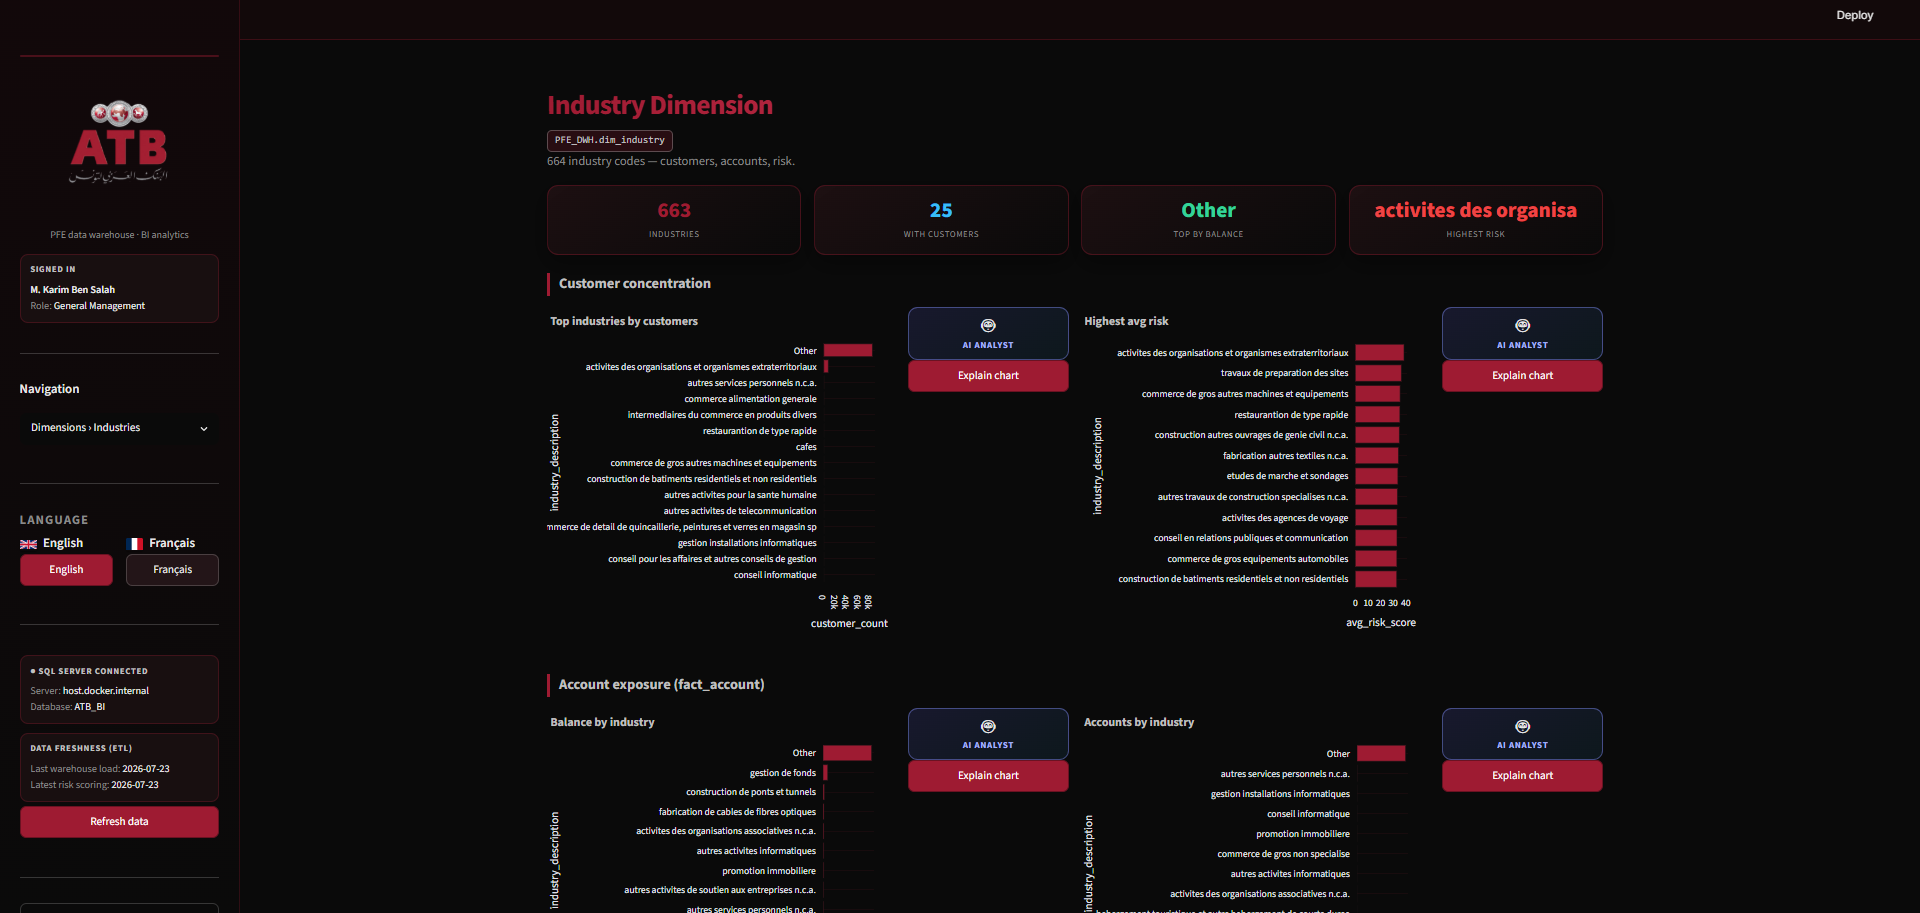
\includegraphics[width=0.88\textwidth]{figures/dash_dim_industry.png}
\caption{Industry dimension concentration bars and risk-vs-volume bubble}
\label{fig:dash_dim_industry}
\end{figure}
\noindent Industry pages drill one level finer than sectors:
concentration bars and risk-vs-volume bubbles isolate activity niches that
drive portfolio risk without drowning the committee in the full NACE catalog.

\begin{figure}[H]
\centering
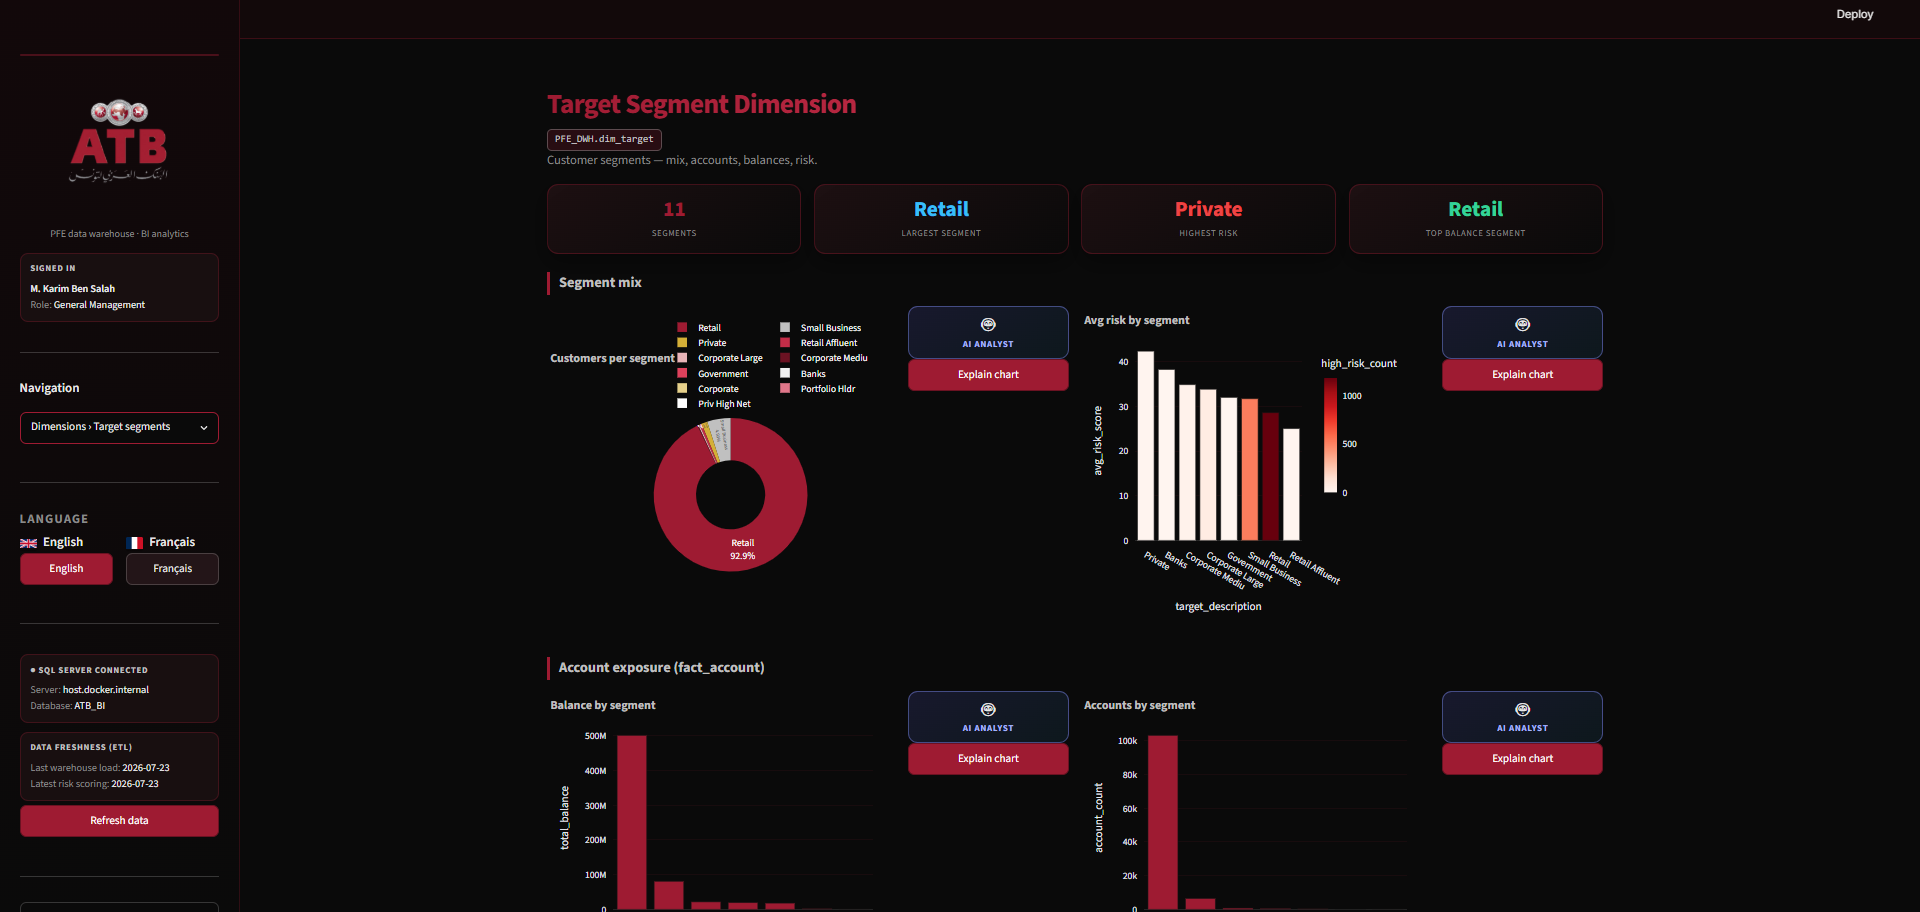
\includegraphics[width=0.88\textwidth]{figures/dash_dim_target.png}
\caption{Target segment dimension segment}
\label{fig:dash_dim_target}
\end{figure}
\noindent Commercial segments (retail, affluent, SME, corporate,
government) are compared on mix, average risk and balance so product and risk
teams share one vocabulary for book quality.

\begin{figure}[H]
\centering
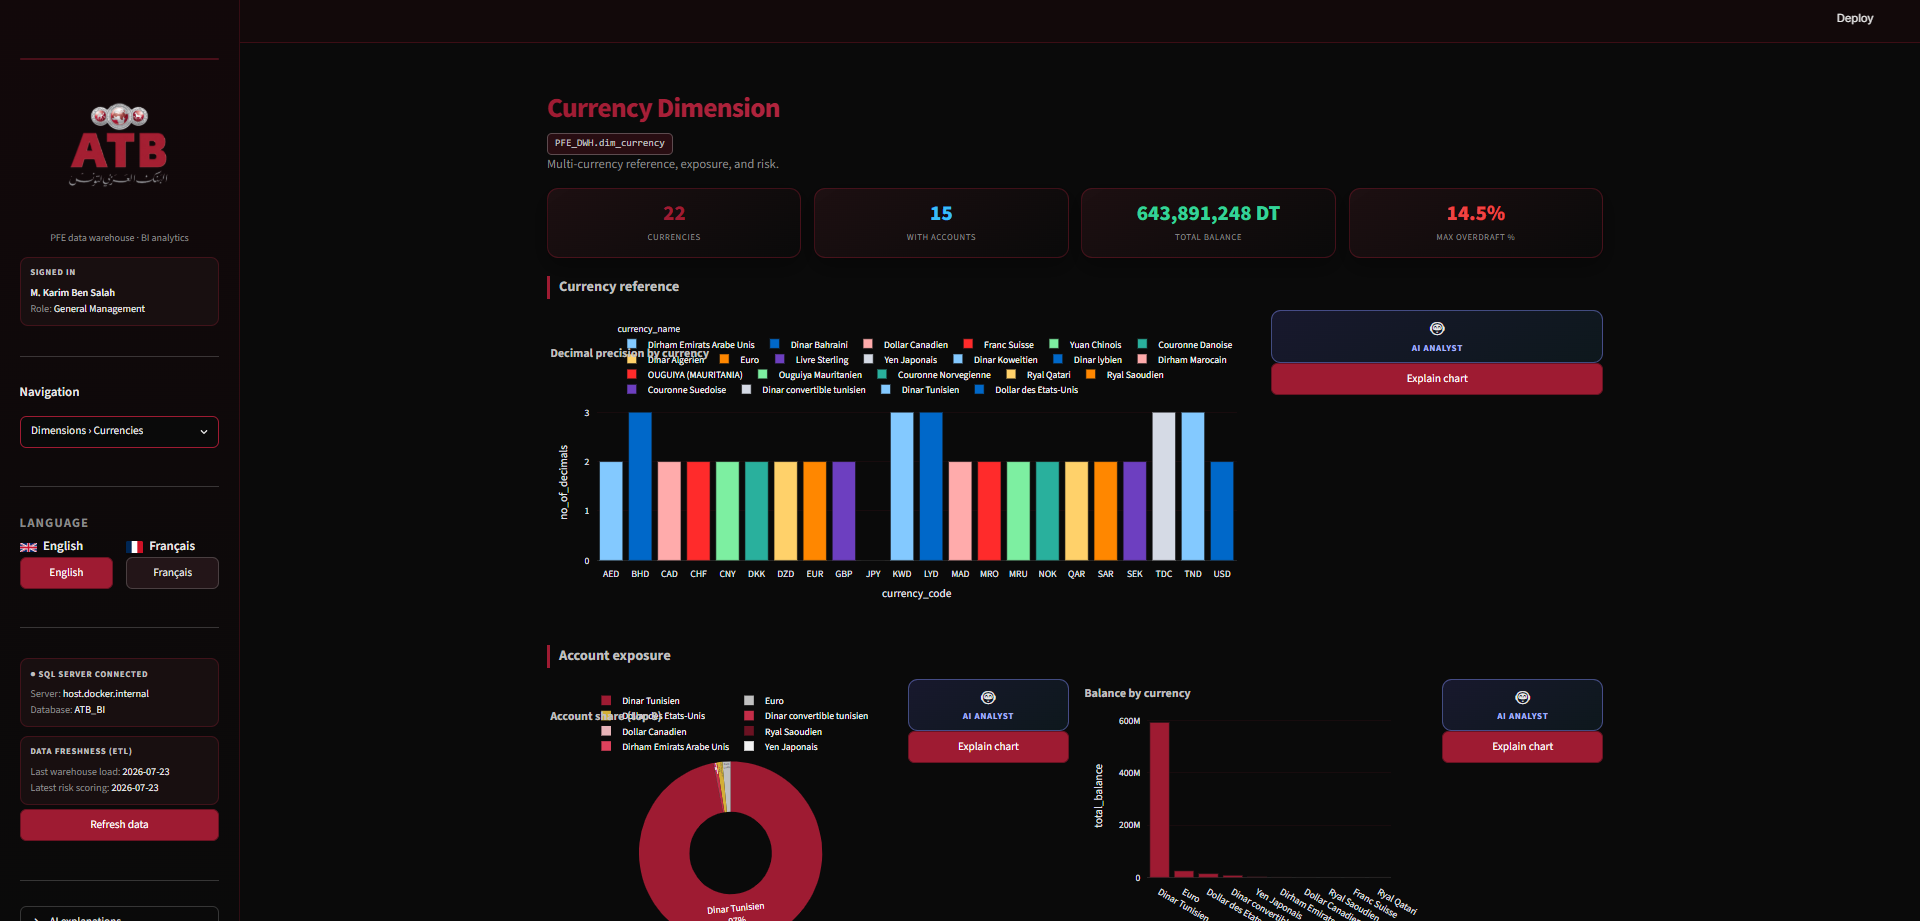
\includegraphics[width=0.88\textwidth]{figures/dash_dim_currency.png}
\caption{Currency dimension balance treemap}
\label{fig:dash_dim_currency}
\end{figure}
\noindent Multi-currency exposure, overdraft and risk by FX code
are summarised with a balance treemap essential when most balances sit in
TND but foreign-currency pockets still matter for ALM.

\begin{figure}[H]
\centering
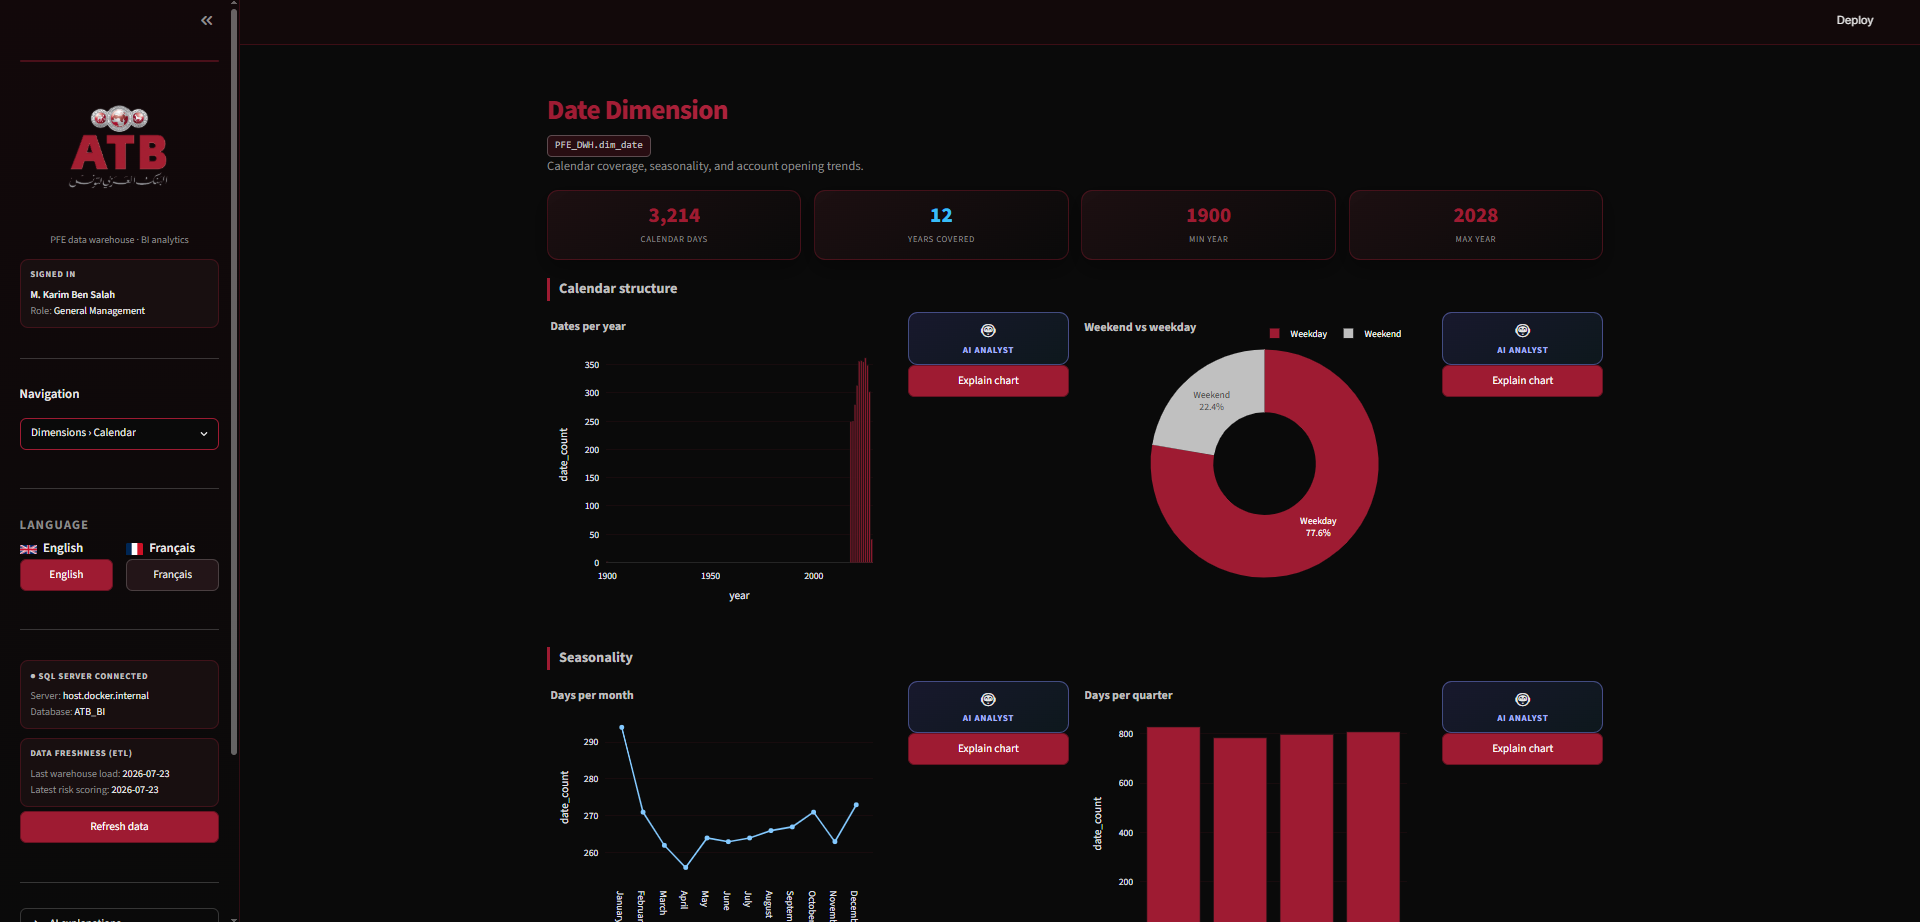
\includegraphics[width=0.88\textwidth]{figures/dash_dim_date.png}
\caption{Calendar dimension}
\label{fig:dash_dim_date}
\end{figure}
\noindent The date dimension turns openings and balances into a
vintage view: growth years, ageing cohorts and seasonality become visible
without exporting raw fact tables to Excel.

\paragraph{Extended KPI catalogue (facts + dimensions).}
Beyond the executive cards, the presentation layer surfaces the fuller set of
indicators prepared in Phase~2:

\begin{table}[H]
\centering
\caption{Extended KPI catalogue available across Streamlit pages}
\label{tab:extended_kpi_catalog}
\renewcommand{\arraystretch}{1.15}
\scriptsize
\begin{tabular}{|p{4.2cm}|p{4.0cm}|p{5.8cm}|}
\hline
\rowcolor{blue!15}
\textbf{KPI} & \textbf{Primary page(s)} & \textbf{Business reading} \\
\hline
Total customers / accounts & Overview, Customers & Book size \\
\hline
Total / average working balance & Overview, Accounts, DAO, Sector & Exposure and wallet size \\
\hline
Overdraft count \& rate & Overview, Accounts, DAO, Sector, Currency & Solvency pressure \\
\hline
Average GRS \& tier mix & Overview, Risk & Portfolio health \\
\hline
High-risk customer count / \% & Overview, Risk, Sector, Target & Priority follow-up mass \\
\hline
Mean CRI / FFS / BRS & Risk & Why the score is high \\
\hline
KYC completion \% & Overview, Compliance, Customers & Regulatory readiness \\
\hline
PEP \% \& flagged \% & Compliance, Customers & Enhanced due diligence load \\
\hline
Avg salary \& salary-band mix & Customers, Studies & Income fragility context \\
\hline
Avg tenure \& tenure bands & Customers, Studies & Relationship maturity \\
\hline
Employment / marital / gender mix & Customers & Demographic steering \\
\hline
Balance \& risk by DAO area & DAO, Comparison & Geographic concentration \\
\hline
Balance, risk, overdraft by sector/industry & Sector, Industry, Comparison & Activity concentration \\
\hline
Segment mix \& segment risk & Target & Commercial book quality \\
\hline
Openings \& balance by vintage year & Calendar & Growth and ageing of the book \\
\hline
FX exposure \& FX overdraft & Currency & Multi-currency risk \\
\hline
ETL freshness timestamp & Overview & Trust in the numbers \\
\hline
\end{tabular}
\end{table}

\subsection{Actionable Features and Sharing}
In line with GIMSI Phase~4 publication requirements, the interface is not limited
to passive charts:
\begin{itemize}
    \item \textbf{Visual alerting:} colour badges and alert inbox entries for
          incomplete KYC, PEP and high GRS;
    \item \textbf{Export / publication:} CSV downloads of filtered lists and
          executive PDF packs (disabled for read-only \texttt{AUDIT});
    \item \textbf{Manual cache refresh:} staff can invalidate TTL caches when an
          urgent recompute is required after an exceptional pipeline run.
\end{itemize}
\begin{figure}[H]
\centering
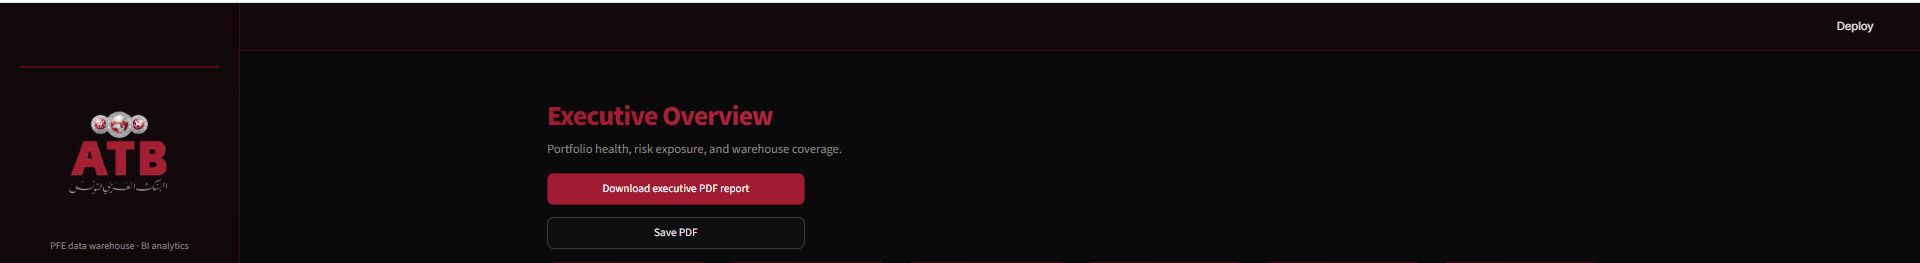
\includegraphics[width=0.75\textwidth]{figures/dash_export_csv.png}
\caption{CSV download button and exported filtered customer list}
\label{fig:dash_export_csv}
\end{figure}
\noindent Filtered risk or compliance lists leave the dashboard
as CSV for offline review disabled for the read-only \texttt{AUDIT} role.

\begin{figure}[H]
\centering
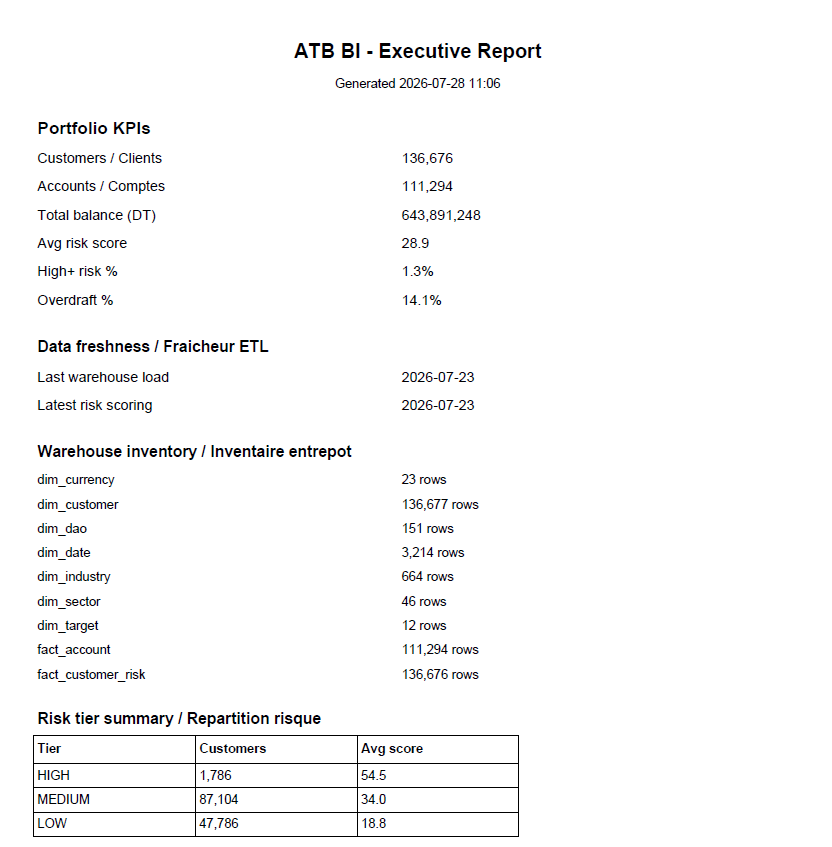
\includegraphics[width=0.75\textwidth]{figures/dash_export_pdf.png}
\caption{Executive PDF report preview}
\label{fig:dash_export_pdf}
\end{figure}
\noindent The executive PDF pack packages the overview KPIs and
key charts into a shareable artefact for committee circulation (GIMSI Phase~4
publication).

\begin{figure}[H]
\centering
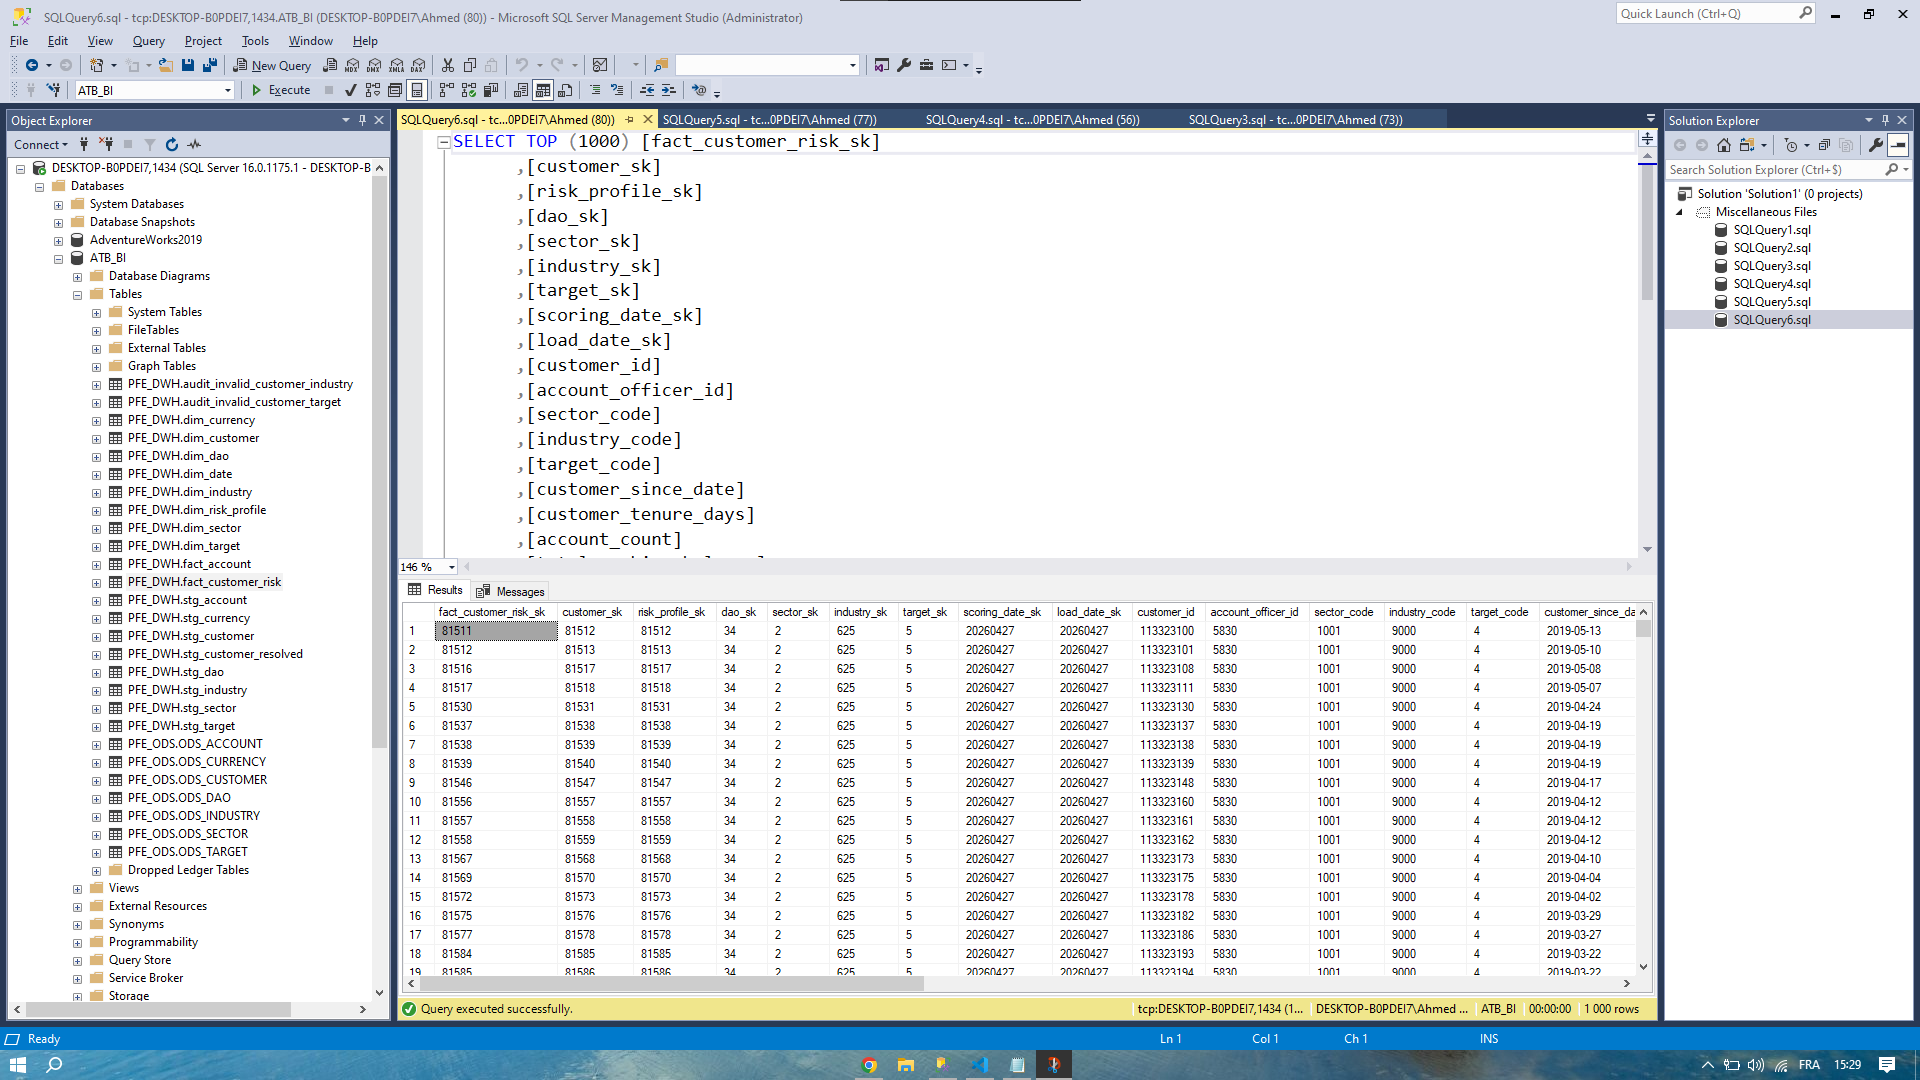
\includegraphics[width=0.88\textwidth]{figures/ssms_pfe_dwh.png}
\caption{SSMS Object Explorer --- \texttt{PFE\_DWH} dimensions and fact tables}
\label{fig:ssms_pfe_dwh}
\end{figure}
\noindent The constellation schema in SQL Server is the single
source of truth behind every Streamlit page shown above.

\begin{figure}[H]
\centering
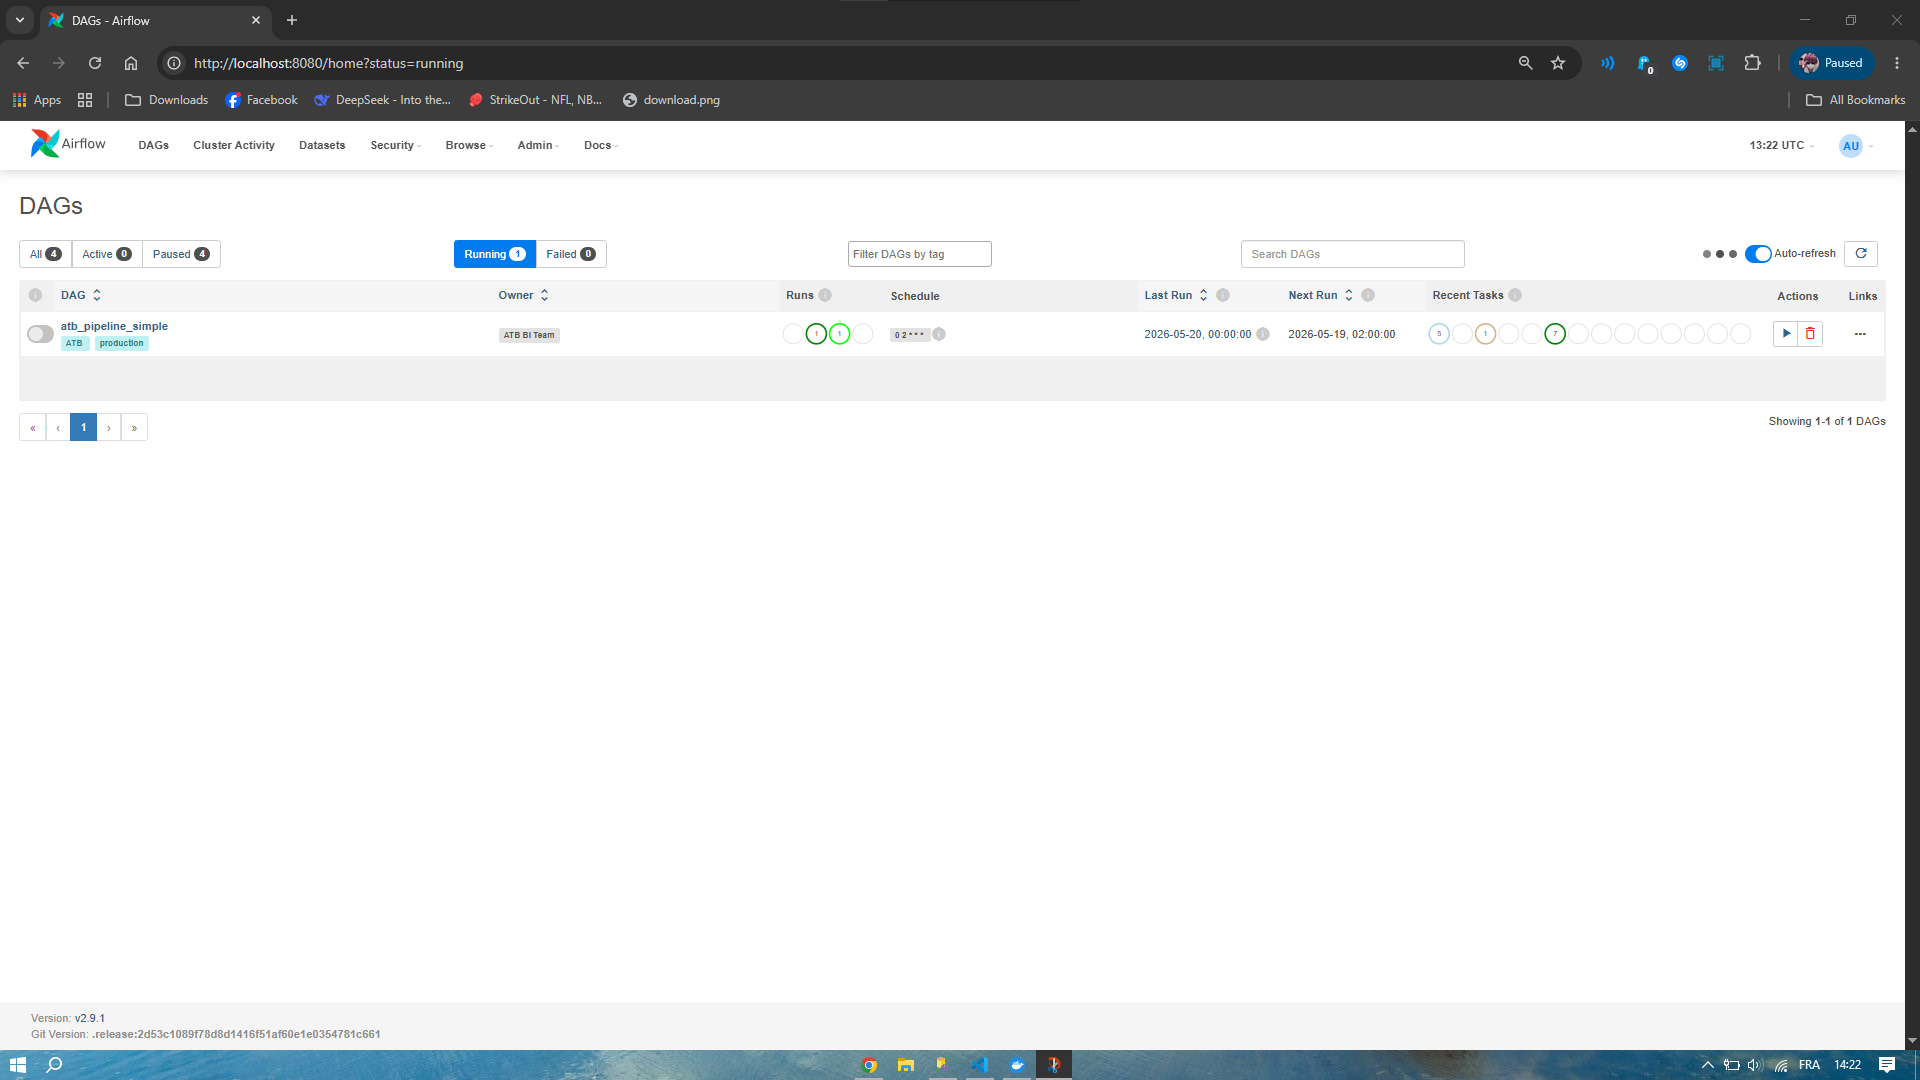
\includegraphics[width=0.88\textwidth]{figures/airflow_master_dag.png}
\caption{Airflow DAG graph view of Master pipeline}
\label{fig:airflow_master_dag}
\end{figure}
\noindent Nightly orchestration (ingestion $\rightarrow$ dbt
$\rightarrow$ quality $\rightarrow$ optional ML) keeps the warehouse --- and
therefore the dashboard TTL caches --- aligned with source extracts.

%======================================================================
\section{Phase 4: Evaluation and Continuous Improvement}
\label{sec:gimsi_phase4}
%======================================================================
The last GIMSI phase marks the completion of the decision cycle. Beyond visual
restitution, it evaluates the tool under real conditions and plans continuous
improvements. A decision dashboard loses value if displayed information is stale;
yet querying SQL Server on every click would overload the server and degrade
latency.

\subsection{Refresh Mechanism (Near Real Time)}
We synchronised Streamlit with the Airflow nightly rebuild using
\texttt{@st.cache\_data(ttl=...)} in the data-access layer.

\begin{itemize}
    \item Executive KPI loaders typically use $\mathrm{TTL}=300$~s (5~minutes);
    \item distribution loaders use $\mathrm{TTL}=180$~s (3~minutes);
    \item AI explanations use $\mathrm{TTL}=3600$~s (stable textual tips).
\end{itemize}

\paragraph{Production data life cycle.}
\begin{enumerate}
    \item \textbf{Nightly rebuild (02:00 UTC):} Airbyte + dbt + quality checks
          refresh \texttt{PFE\_DWH}.
    \item \textbf{First morning click:} Streamlit loads fresh warehouse rows into
          cache.
    \item \textbf{Interactive service:} subsequent filters/pages are served from
          memory until TTL expiry.
    \item \textbf{Manual refresh:} operators may clear cache after an exceptional
          recompute.
\end{enumerate}

\begin{figure}[H]
\centering
\begin{tikzpicture}[
  font=\scriptsize,
  step/.style={rectangle, rounded corners=2pt, draw=#1, fill=#1!12, thick,
               align=center, minimum width=2.55cm, minimum height=1.15cm},
  arr/.style={->, thick}
]
  \node[step=teal!70!black] (a) {Airflow\\02:00 UTC};
  \node[step=blue!70!black, right=0.4cm of a] (b) {dbt build\\+ tests};
  \node[step=violet!70!black, right=0.4cm of b] (c) {\texttt{PFE\_DWH}\\fresh facts};
  \node[step=orange!80!black, right=0.4cm of c] (d) {Streamlit\\TTL cache};
  \draw[arr] (a) -- (b);
  \draw[arr] (b) -- (c);
  \draw[arr] (c) -- (d);
\end{tikzpicture}
\caption{Freshness chain --- nightly Airflow rebuild to Streamlit TTL cache}
\label{fig:freshness_chain}
\end{figure}

\subsection{Perspectives for Continuous Improvement}
GIMSI Phase~4 also implies that the decision system must not remain static:
\begin{itemize}
    \item \textbf{Evolutionary KPI adjustment:} new regulatory fields can be added as
          point rules in \texttt{int\_customer\_risk\_score.sql} without redesigning
          the constellation.
    \item \textbf{Periodic technical audits:} monitor ELT duration, index health,
          parse rates and tier-distribution drift.
    \item \textbf{Weight governance:} re-run sensitivity analysis when the risk
          committee changes priorities.
    \item \textbf{Predictive extension:} Release~3 replaces purely descriptive
          steering with supervised models and MLflow tracking on the same warehouse
          features.
\end{itemize}

%======================================================================
\section{Conclusion}
\label{sec:release2_conclusion}
%======================================================================
%----------------------------------------------------------------------
% SCREENSHOT CHECKLIST (commented — capture these, then uncomment includegraphics)
% Save under report/figures/ with the exact names below, then replace the
% nearby %% TODO_SCREENSHOT lines with:
%   \begin{figure}[H]\centering\includegraphics[width=0.85\textwidth]{figures/NAME.png}
%   \caption{...}\label{fig:...}\end{figure}
%
% INGESTION
%   [ ] airbyte_docker_ui.png
%   [ ] airbyte_github_source.png
%   [ ] airbyte_connections_list.png
%   [ ] airbyte_sync_success.png
%   [ ] github_raw_csv.png
% CLEANING
%   [ ] stg_customer_sql.png
%   [ ] dbt_test_pass.png
%   [ ] ods_vs_stg_compare.png
% DASHBOARD CORE
%   [ ] dash_overview_kpis.png
%   [ ] dash_studies.png
%   [ ] dash_compliance.png
%   [ ] dash_alert_inbox.png
%   [ ] dash_risk_pillars.png
%   [ ] dash_accounts.png
%   [ ] dash_rbac_branch.png
%   [ ] dash_ai_explain.png
% DIMENSION PAGES
%   [ ] dash_dim_customer.png
%   [ ] dash_dim_dao.png
%   [ ] dash_dim_sector.png
%   [ ] dash_dim_industry.png
%   [ ] dash_dim_target.png
%   [ ] dash_dim_currency.png
%   [ ] dash_dim_date.png
% EXPORT / OPS
%   [ ] dash_export_csv.png
%   [ ] dash_export_pdf.png
%   [ ] ssms_pfe_dwh.png
%   [ ] airflow_master_dag.png
%----------------------------------------------------------------------
This second iteration (Release~2) transformed raw operational extracts into a
genuine decision-support system. Rigorous application of GIMSI guaranteed an
optimal four-layer structure: from Airbyte acquisition and dbt ELT through a
robust SQL Server constellation warehouse to interactive Streamlit restitution.

At the heart of the architecture, the three-pillar weighted baseline
($40\%$ compliance / $35\%$ financial / $25\%$ behavioural) proved effective and
explainable. Feature-driver analysis empirically validated the business choices by
confirming the predominance of KYC quality, salary/balance pressure and tenure
signals. Central Management, Compliance and Branch Managers now share a visual,
actionable and role-safe cockpit built on $281{,}960$ referentially clean fact
rows.

However, although this heuristic approach offers very satisfactory descriptive
performance, it remains static relative to evolving customer behaviour. The final
project stage (Release~3) will therefore complement the deterministic scoring
engine with Machine Learning models, in order to make risk anticipation
predictive and self-adaptive while reusing the warehouse, KPIs and dashboard
shell already validated here.

%======================================================================
% CHAPTER 5 — RELEASE 3: ARTIFICIAL INTELLIGENCE AND MACHINE LEARNING
%              (SPRINT 4)
% Methodology: CRISP-ML
% Content: ATB Customer Risk ML platform (Jupyter → XGBoost → MLflow → Streamlit)
% Skeleton aligned with supervisor-approved NotMyChapitre5.tex
%======================================================================
\chapter{Release 3: Artificial Intelligence and Machine Learning}
\label{chap:release3}

%----------------------------------------------------------------------
\section{Introduction}
%----------------------------------------------------------------------
Releases~1 and~2 of the ATB BI platform established a secure orchestration engine
(Apache Airflow), a Kimball constellation data warehouse, and an
interactive Streamlit decision dashboard driven by a transparent three-pillar rules
engine. \textbf{Release~3 --- Sprint~4} constitutes the qualitative leap from
\emph{descriptive} steering to \emph{predictive} intelligence: complementing the
auditable warehouse score with a supervised Machine Learning layer that screens
customers, surfaces disagreement alerts, and exposes model quality to risk managers
in real time.

This sprint delivers four interconnected innovations:
\begin{enumerate}
    \item \textbf{CRISP-ML lifecycle} applied end-to-end: from business understanding
          through Jupyter exploratory analysis, model engineering, MLflow tracking,
          and production deployment inside the existing dashboard shell.
    \item \textbf{XGBoost production classifier} trained on warehouse features
          (KYC, balances, sector, tenure) to predict $P(\text{high risk})$ where
          \texttt{high risk} $\equiv$ \texttt{global\_risk\_score} $\geq 50$.
    \item \textbf{Dual-layer risk architecture}: the rules engine remains the official
          auditable score; ML acts as a screening assistant that flags cases where
          model and rules diverge.
    \item \textbf{Operational integration}: nightly/weekly Airflow retraining,
          batch scoring into the \texttt{PFE\_ML} warehouse schema, and a
          five-tab \emph{ML Risk Intelligence} Streamlit module (live demo, batch
          alerts, curves \& SHAP, metrics, full predictor).
\end{enumerate}

Sprint~4 directly addresses User Stories US~10 to US~14 defined in
Chapter~2: train the algorithm, consult predictions, read curve interpretations,
compare risk by sector/zone, and export predictive scores.

%======================================================================
\section{Adoption of the CRISP-ML Methodology}
\label{sec:crispml_adoption}
%======================================================================

Global project governance remains \textbf{Scrum} (three-week sprints, prioritised
backlog, sprint reviews). For the AI/ML component of Sprint~4, this governance was
reinforced by \textbf{CRISP-ML} (\textit{Cross-Industry Standard Process for Machine
Learning}), the extension of CRISP-DM with explicit model-quality and deployment
phases already introduced in Chapter~1.

CRISP-ML provides three guarantees absent from an ad hoc notebook workflow:
\begin{itemize}
    \item \textbf{Full traceability}: every feature choice, hyperparameter, and
          performance threshold is logged in MLflow (\texttt{4\_ml/mlruns/}).
    \item \textbf{Integrated quality assurance}: acceptance gates (F1 $\geq 0.70$,
          ROC-AUC $\geq 0.80$) are defined \emph{before} declaring a model
          production-ready.
    \item \textbf{Reproducibility}: the pipeline is entirely scripted
          (\texttt{run\_training.py}, five ordered Jupyter notebooks); a
          \texttt{git pull} plus warehouse connection suffices to regenerate
          artefacts.
\end{itemize}

\subsection{The Six CRISP-ML Phases Applied to Sprint~4}

\begin{table}[H]
\centering
\caption{CRISP-ML phase mapping $\leftrightarrow$ Sprint~4 deliverables}
\label{tab:crispml-mapping-atb}
\begin{tabular}{|c|l|l|}
\hline
\textbf{Phase} & \textbf{CRISP-ML name} & \textbf{Sprint~4 deliverable} \\
\hline
1 & Business Understanding & Dual-layer rules + ML architecture (US~10--14) \\
2 & Data Understanding \& Preparation & 5 Jupyter notebooks + leakage-safe features \\
3 & Model Engineering & XGBoost + 3 baselines, SMOTETomek, MLflow runs \\
4 & Model Evaluation & ROC/PR, confusion matrix, SHAP, overfitting checks \\
5 & Model Deployment & Streamlit \emph{ML Risk Intelligence} + \emph{MLflow Registry} pages \\
6 & Monitoring \& Maintenance & Airflow \texttt{dag\_ml\_pipeline}, Docker, batch scoring \\
\hline
\end{tabular}
\end{table}
%======================================================================
\section{Business Understanding}
\label{sec:phase1_business}
%======================================================================

\subsection{Problem Statement and Objectives}

Phase~1 formalises the needs of ATB risk stakeholders \emph{before} any modelling.
Two complementary business challenges guided the architecture:

\begin{enumerate}
    \item \textbf{Instant high-risk screening}: compliance officers and branch risk
          managers must identify fragile profiles in seconds, not after a manual
          spreadsheet review.
    \item \textbf{Early warning beyond static rules}: the three-pillar warehouse
          score (\texttt{global\_risk\_score}) is explainable but rule-bound; ML
          must learn non-linear patterns (overdraft behaviour, stale KYC, salary
          pressure) that precede tier escalation.
\end{enumerate}

\subsection{Dual-Layer Decision Architecture}

Rather than replacing the GIMSI-validated rules engine, we designed a
\textbf{dual-layer} architecture where each layer has a distinct responsibility:

\begin{table}[H]
\centering
\caption{Dual-layer architecture --- roles and responsibilities}
\label{tab:dual-layer-roles}
\begin{tabular}{|l|p{5.2cm}|p{5.2cm}|}
\hline
\textbf{Dimension} & \textbf{Rules engine (DWH)} & \textbf{XGBoost ML} \\
\hline
Task & Deterministic 3-pillar scoring & Binary classification $P(\text{high risk})$ \\
Output & \texttt{global\_risk\_score} [0--100] + \texttt{risk\_tier} & Probability $\in [0,1]$ + label \\
Threshold & Fixed: score $\geq 50$ & Optimised on F1 (production $\approx 0.953$) \\
Inputs & Compliance / financial / behavioural indices & 34+ customer attributes (no score leakage) \\
Role & Official auditable score & Screening assistant + disagreement alerts \\
Usage & Regulatory reporting, KPI dashboards & On-demand in Streamlit + nightly batch \\
\hline
\end{tabular}
\end{table}

The Streamlit banner (\texttt{ml\_page.py}) makes this contract explicit to end
users: rules compute the official score; ML predicts high risk from attributes and
highlights cases requiring manual review when the two layers disagree.

\subsection{A Priori Acceptance Criteria (CRISP-ML Quality Gate)}

In line with CRISP-ML, acceptance thresholds were fixed \emph{before} the final
training run (documented in \texttt{FULL\_INTEGRATION\_STATUS.md}):
\begin{itemize}
    \item \textbf{F1 score} (test) $\geq 0.70$
    \item \textbf{ROC-AUC} (test) $\geq 0.80$
    \item \textbf{PR-AUC} monitored (critical given class imbalance $\approx 1.3\%$ positives)
    \item \textbf{Train--test F1 gap} $< 10\%$ (overfitting control)
    \item \textbf{No target leakage}: \texttt{global\_risk\_score}, pillar indices,
          and \texttt{risk\_tier} are explicitly excluded in
          \texttt{features.py}.
\end{itemize}

%======================================================================
\section{Data Understanding \& Preparation}
\label{sec:phase2_data}
%======================================================================

\subsection{Exploratory Data Analysis}

Before building any model, a five-notebook analysis pipeline was carried out
to understand the data, identify risks (such as class imbalance and target
leakage), and guide feature engineering choices.

\begin{table}[H]
\centering
\caption{Analysis notebook pipeline --- Sprint~4}
\label{tab:notebook-pipeline}
\begin{tabular}{|c|p{4cm}|p{7cm}|}
\hline
\textbf{\#} & \textbf{Notebook} & \textbf{Purpose} \\
\hline
01 & Data Profiling & Class balance, missing values, leakage audit \\
02 & Feature Engineering & Derived indicators, temporal train/test split \\
03 & Model Training & Four algorithms benchmarked and tracked \\
04 & SHAP Explainability & Global and local feature importance plots \\
05 & Model Selection & Final metric grid and production decision \\
\hline
\end{tabular}
\end{table}

\textbf{Data source.} The model is trained on customer records extracted from
the data warehouse, joining transaction facts with customer dimension attributes.
The full population contains 281{,}960 records, of which up to 5{,}000 are
sampled for iterative training runs.

\textbf{Binary target construction:}
\begin{equation}
\text{risk\_target} =
\begin{cases}
1 & \text{if } \texttt{global\_risk\_score} \geq 50 \quad (\text{high risk}) \\
0 & \text{otherwise}
\end{cases}
\label{eq:risk-target}
\end{equation}

\textbf{Class imbalance.} The exploratory analysis reveals a strongly imbalanced
target: only approximately \textbf{1.3\%} of customers are classified as high-risk.
This motivates the use of SMOTETomek resampling and prioritises F1 score, recall,
and PR-AUC over raw accuracy as evaluation criteria.

% --- SCREENSHOT: copy 4_ml/outputs/eda_target_and_distribution.png → figures/
\begin{figure}[H]
\centering
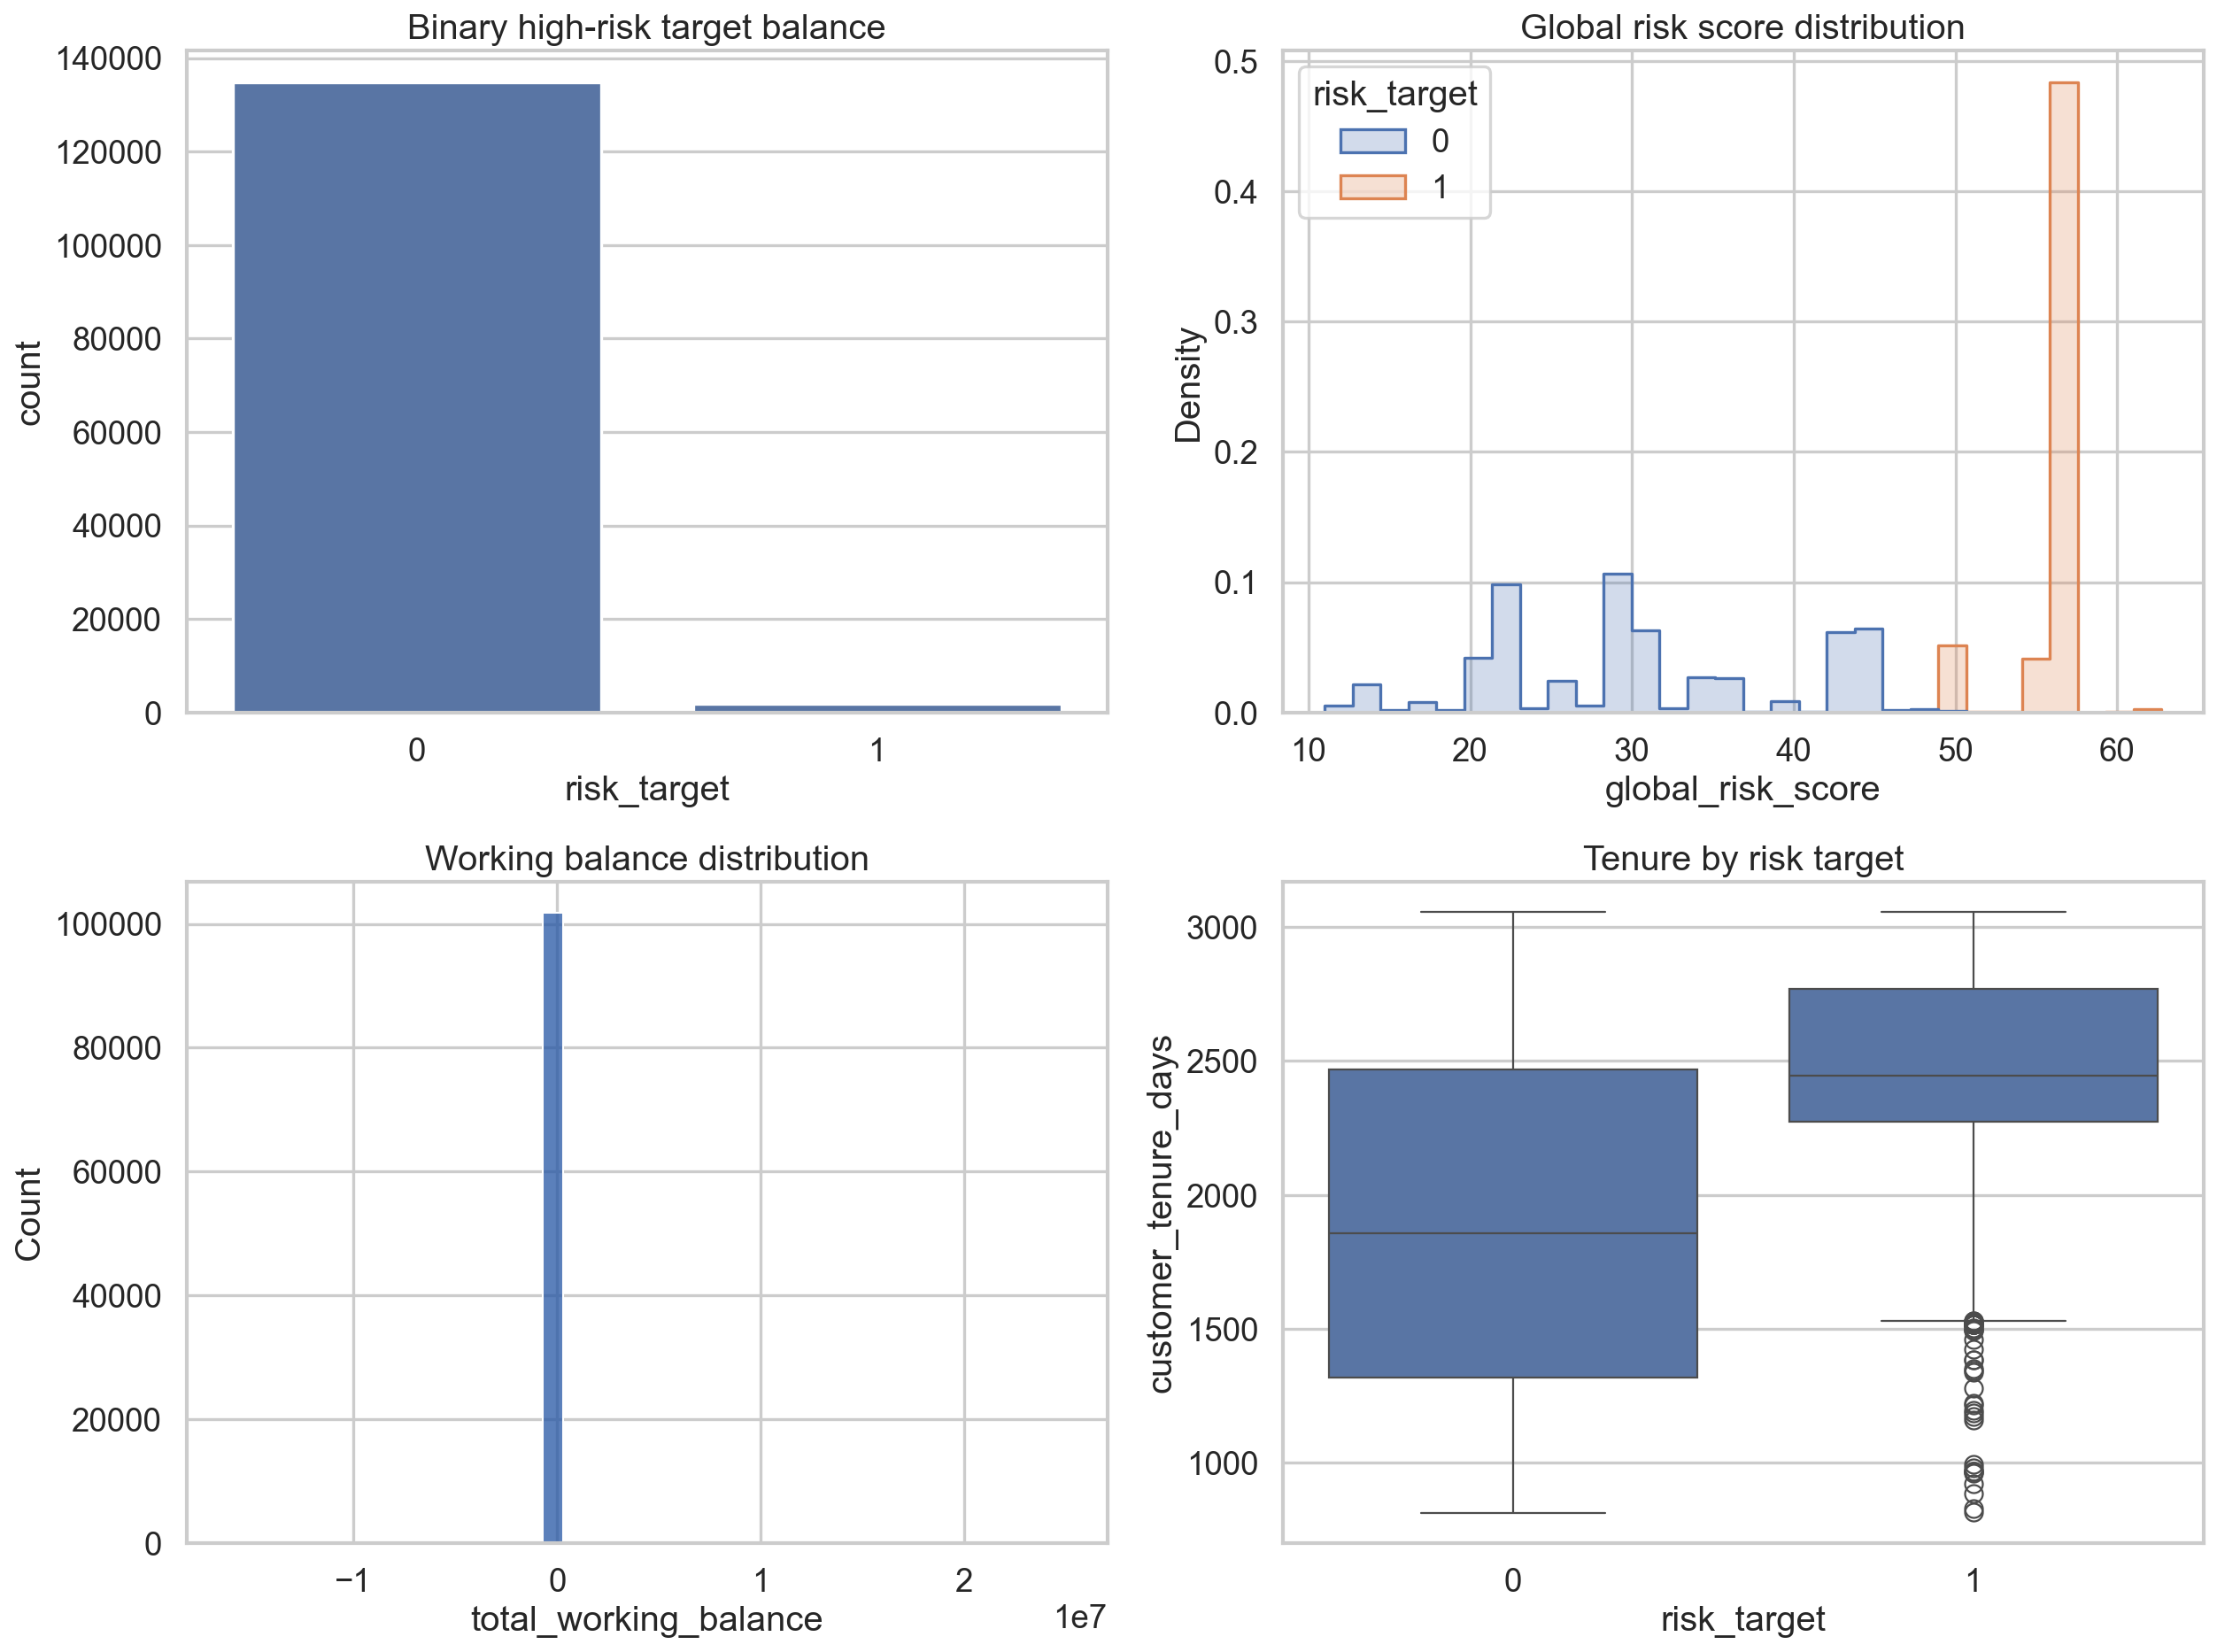
\includegraphics[width=0.75\textwidth]{figures/eda_target_and_distribution.png}
\caption{EDA distribution of global risk score and binary target balance}
\label{fig:eda-target-dist}
\end{figure}
\noindent The continuous GRS mass sits well below 50; the binary
cut at 50 yields only $\approx 1.3\%$ positives hence F1, recall and PR-AUC
dominate accuracy in later evaluation.

% --- SCREENSHOT: copy 4_ml/outputs/eda_correlation_heatmap.png → figures/
\begin{figure}[H]
\centering
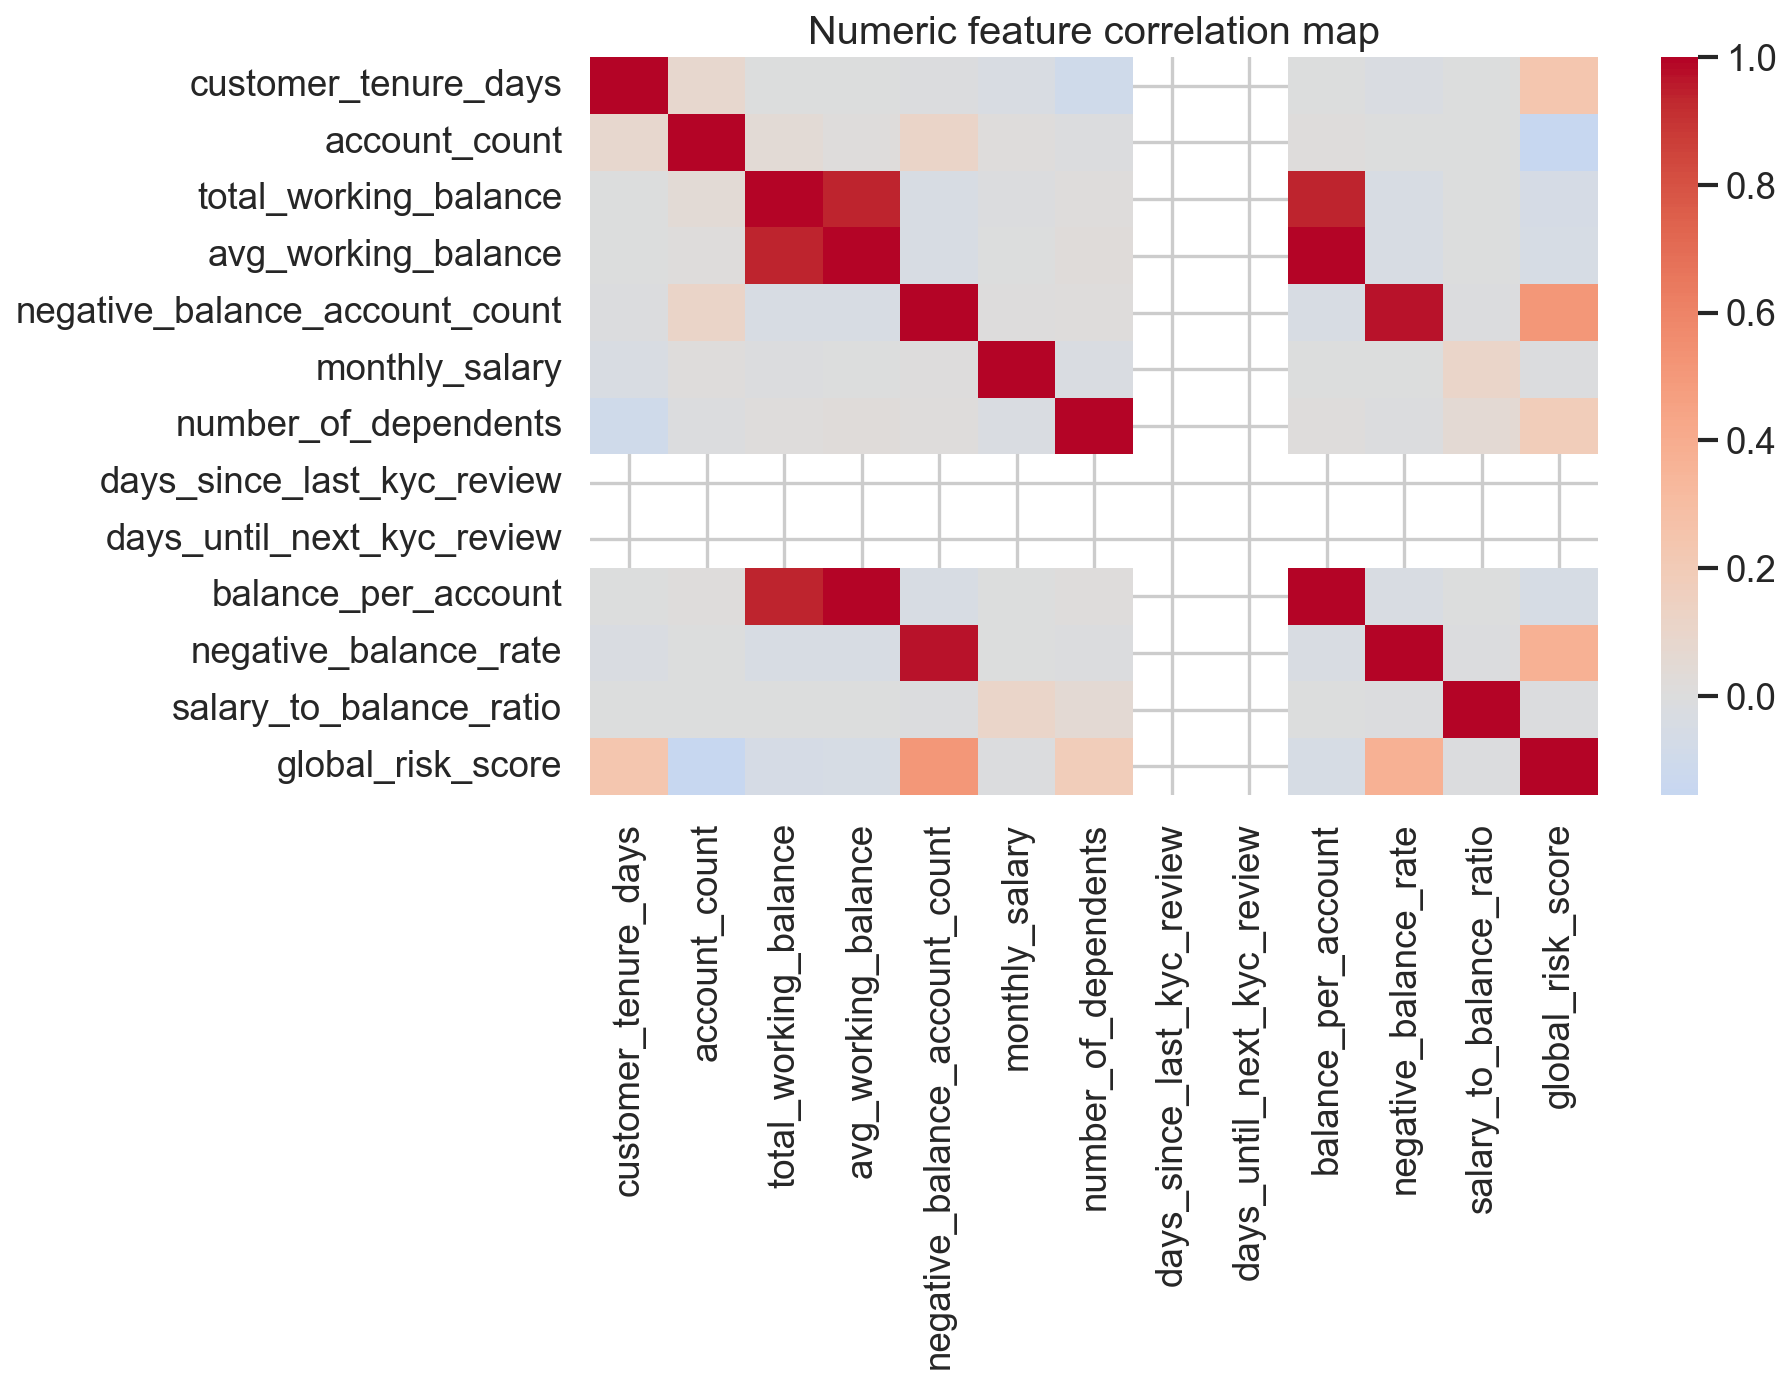
\includegraphics[width=0.75\textwidth]{figures/eda_correlation_heatmap.png}
\caption{EDA correlation heatmap of numeric risk drivers}
\label{fig:eda-corr}
\end{figure}
\noindent Weak linear correlations among demographics confirm
that tree ensembles are a better inductive bias than a purely linear separator.

Key EDA findings that shaped feature engineering:
\begin{itemize}
    \item \textbf{KYC staleness} is strongly associated with elevated compliance
          risk; customers with outdated identity records are more likely to appear
          in the high-risk class.
    \item \textbf{Financial stress signals} such as overdraft frequency and
          a high salary-to-balance ratio clearly separate the high-risk tail
          from the general population.
    \item \textbf{Low linear correlations} between raw demographic attributes
          confirm that tree-based, non-linear models are the most appropriate
          family for this classification task.
\end{itemize}

\subsection{Feature Engineering and Variable Selection}

A total of \textbf{34 input features} are fed to the model, organised into
three functional categories. To prevent \emph{target leakage}, the warehouse
risk score, its three component indices, and the risk tier label are
explicitly excluded from the feature set.

The engineered indicators below are computed from raw warehouse fields and
capture key dimensions of customer risk:

\begin{table}[H]
\centering
\caption{Engineered features and their business meaning}
\label{tab:engineered-features}
\begin{tabular}{|p{4.8cm}|l|p{5.5cm}|}
\hline
\textbf{Feature} & \textbf{Type} & \textbf{Business meaning} \\
\hline
Days since last KYC review & Numeric & Time elapsed since regulatory identity check \\
Has overdraft & Binary & Whether the customer holds any overdrawn account \\
Negative balance rate & Numeric & Share of accounts currently in negative balance \\
Salary-to-balance ratio & Numeric & Income relative to liquidity; signals financial pressure \\
KYC stale / very stale & Binary & Review overdue by more than 1 or 2 years \\
Is new customer & Binary & Tenure below 12 months \\
Balance per account & Numeric & Average balance across all held accounts \\
\hline
\end{tabular}
\end{table}

In addition, the model uses four \textbf{compliance flags} drawn directly
from the warehouse: KYC completeness status, politically exposed person (PEP)
status, a general compliance flag, and the presence of an active compliance
decision. Finally, \textbf{demographic and segmentation attributes} such as
employment status, gender, marital and residence status, branch area, sector,
industry, and customer segment are included, bringing the feature total to 34.

\subsection{Preprocessing Pipeline}

\begin{table}[H]
\centering
\caption{Preprocessing steps applied before model training}
\label{tab:preprocessing}
\begin{tabular}{|l|p{9cm}|}
\hline
\textbf{Step} & \textbf{Description} \\
\hline
Imputation & Median substitution for numeric fields; most-frequent value for categoricals \\
Encoding & One-hot encoding for all categorical variables; unknown categories ignored at inference \\
Scaling & Standard normalisation applied for Logistic Regression only \\
Class balancing & SMOTETomek applied after encoding, before classifier fitting \\
Temporal split & 80\% training / 20\% test, ordered chronologically to prevent data leakage \\
\hline
\end{tabular}
\end{table}

%======================================================================
\section{Model Engineering}
\label{sec:phase3_modeling}
%======================================================================

\subsection{Experiment Tracking with MLflow}

All training experiments are tracked using \textbf{MLflow}. Each algorithm
produces a separate logged run containing its hyperparameters, performance
metrics, and a serialised model artefact. The best-performing model is
registered under the name \texttt{Customer Risk Classifier } and
promoted to the \textbf{Production} stage, making it available to the
dashboard without any manual file handling.

\begin{figure}[H]
\centering
\resizebox{\linewidth}{!}{%
\begin{tikzpicture}[
  node distance=0.4cm and 0.8cm,
  every node/.style={font=\small},
  box/.style={rectangle, rounded corners=3pt, draw=black!60, fill=blue!8,
              minimum width=2.4cm, minimum height=0.75cm, align=center},
  arrow/.style={->, thick, draw=black!60},
  note/.style={font=\footnotesize\itshape, text width=2.4cm, align=center}
]
\node[box] (train) {Train};
\node[box, right=of train] (log) {Log run};
\node[box, right=of log] (reg) {Register};
\node[box, right=of reg] (prod) {Promote to\\Production};
\node[box, right=of prod] (score) {Batch score};

\draw[arrow] (train) -- (log);
\draw[arrow] (log) -- (reg);
\draw[arrow] (reg) -- (prod);
\draw[arrow] (prod) -- (score);

\node[note, below=0.2cm of train] {Hyperparameters\\+ metrics logged};
\node[note, below=0.2cm of log] {Run stored in\\MLflow experiment};
\node[note, below=0.2cm of reg] {Model registered\\with version tag};
\node[note, below=0.2cm of prod] {Previous version\\archived};
\node[note, below=0.2cm of score] {Predictions written\\to warehouse};
\end{tikzpicture}%
}
\caption{MLflow model lifecycle: from training run to warehouse-persisted predictions}
\label{fig:mlflow-lifecycle}
\end{figure}
\noindent Every experiment is a logged run; only the winning
artefact is registered, promoted to Production, then used for batch scoring.

\subsection{Benchmark: Four Supervised Classifiers}

Four classifiers were evaluated under identical conditions: same 34-feature input
set, same SMOTETomek-balanced training split, same stratified 2-fold
with F1 as the optimisation metric, and the same
temporal test holdout . Each run was
individually logged in MLflow so that artefacts, hyperparameters, and metrics
are fully reproducible.

\begin{table}[H]
\centering
\caption{Comprehensive four-model comparison test-set metrics}
\label{tab:all-models-comparison}
\renewcommand{\arraystretch}{1.25}
\begin{tabular}{|l|c|c|c|c|c|c|c|}
\hline
\textbf{Model} & \textbf{Accuracy} & \textbf{F1} & \textbf{Precision} & \textbf{Recall} & \textbf{ROC-AUC} & \textbf{PR-AUC} & \textbf{Brier} \\
\hline
\textbf{XGBoost} & \textbf{0.9988} & \textbf{0.9545} & 0.9130 & \textbf{1.0000} & \textbf{1.0000} & \textbf{1.0000} & \textbf{0.0013} \\
Random Forest & 0.9975 & 0.8947 & \textbf{1.0000} & 0.8095 & 0.9998 & 0.9908 & 0.0024 \\
Extra Trees & 0.9869 & 0.5333 & 0.8000 & 0.4000 & 0.9960 & 0.8200 & 0.0131 \\
Logistic Regression & 0.9931 & 0.7556 & 0.7083 & 0.8095 & 0.9977 & 0.8137 & 0.0065 \\
\hline
\end{tabular}
\end{table}

\textbf{Reading the table.}
\begin{itemize}
    \item \textbf{XGBoost} dominates on every metric that matters for imbalanced
          screening: F1 (+6.0 pp over Random Forest), perfect recall (zero missed
          high-risk cases), and a Brier score five times lower than Logistic Regression.
    \item \textbf{Random Forest} achieves perfect precision (no false alarms) but
          sacrifices recall (19\% of high-risk customers missed) unacceptable
          when the business objective is exhaustive screening.
    \item \textbf{Extra Trees} achieves high ROC-AUC yet collapses on F1 (0.53),
          reflecting an over-randomised structure that degrades recall at the
          production threshold. It was rejected despite passing the ROC gate.
    \item \textbf{Logistic Regression} provides a respectable linear baseline
          (F1 $= 0.76$) but cannot capture the non-linear interaction between
          PEP status, KYC staleness, and overdraft behaviour.
\end{itemize}

\subsection{Pairwise Analysis: XGBoost vs.\ Logistic Regression}

Logistic Regression is the natural interpretable baseline: it is fast, transparent,
and requires no hyperparameter tuning. However, it is limited to linear decision
boundaries and cannot capture compound risk patterns.

Test-set results:

\begin{table}[H]
\centering
\caption{Classification XGBoost vs.\ Logistic Regression (test set)}
\label{tab:xgb-vs-lr}
\begin{tabular}{|l|c|c|c|}
\hline
\textbf{Metric} & \textbf{XGBoost} & \textbf{Logistic Regression} & \textbf{Gain} \\
\hline
Accuracy & \textbf{0.9988} & 0.9931 & +0.6 pp \\
F1 & \textbf{0.9545} & 0.7556 & +19.9 pp \\
Precision & 0.9130 & 0.7083 & +20.5 pp \\
Recall & \textbf{1.0000} & 0.8095 & +19.1 pp \\
ROC-AUC & \textbf{1.0000} & 0.9977 & +0.2 pp \\
PR-AUC & \textbf{1.0000} & 0.8137 & +18.6 pp \\
Brier score & \textbf{0.0013} & 0.0065 & $-$80\% \\
\hline
\end{tabular}
\end{table}

XGBoost captures compound non-linear patterns (e.g.\ PEP status combined with
stale KYC and overdraft behaviour) that logistic weights cannot represent. The
F1 margin of \textbf{+19.9 pp} and a Brier score five times lower confirm that
XGBoost is the superior production choice.

% --- SCREENSHOT: copy 4_ml/outputs/03_model_comparison_bars.png
\begin{figure}[H]
\centering
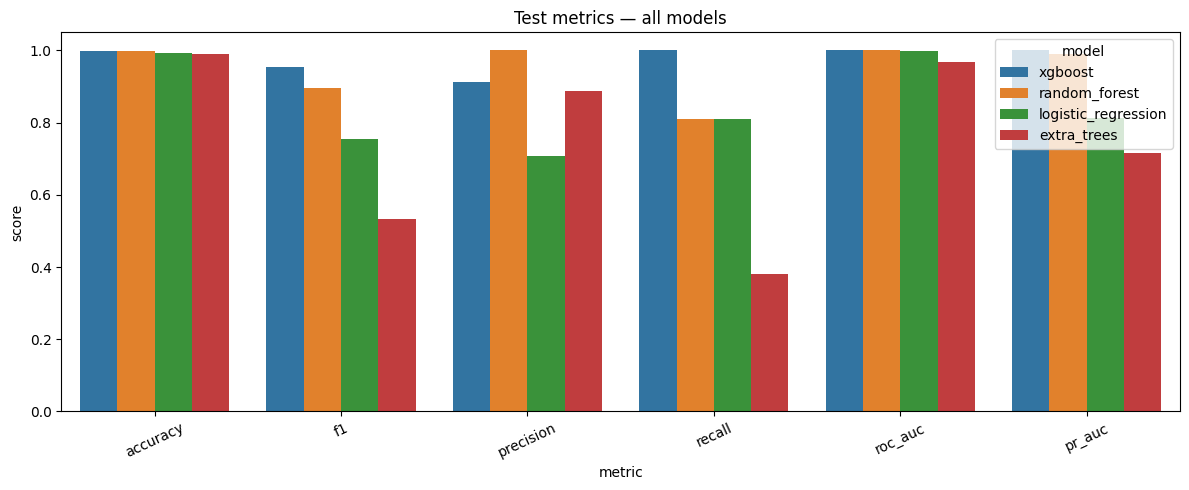
\includegraphics[width=0.92\textwidth]{figures/03_model_comparison_bars.png}
\caption{Bar chart comparing four algorithms on test F1 and ROC-AUC}
\label{fig:model-comparison-bars}
\end{figure}
\noindent Visual confirmation of Table~\ref{tab:all-models-comparison}:
XGBoost leads on F1 while all four models score high ROC-AUC --- F1 is therefore
the discriminating gate under imbalance.

\subsection{Pairwise Analysis: XGBoost vs.\ Random Forest}

\begin{table}[H]
\centering
\caption{Classification --- XGBoost vs.\ Random Forest (test set)}
\label{tab:xgb-vs-rf}
\begin{tabular}{|l|c|c|c|}
\hline
\textbf{Metric} & \textbf{XGBoost} & \textbf{Random Forest} & \textbf{Comment} \\
\hline
F1 & \textbf{0.9545} & 0.8947 & XGBoost +6.0 pp \\
Precision & 0.9130 & \textbf{1.0000} & RF more conservative on positives \\
Recall & \textbf{1.0000} & 0.8095 & XGBoost catches all test high-risk cases \\
ROC-AUC & \textbf{1.0000} & 0.9998 & Both excellent ranking \\
PR-AUC & \textbf{1.0000} & 0.9908 & Critical under 1.3\% prevalence \\
Optimal threshold & 0.953 & 0.612 & F1-optimised per model \\
\hline
\end{tabular}
\end{table}

Random Forest achieves perfect precision but sacrifices recall unacceptable
when the business goal is to \emph{screen} high-risk customers. XGBoost balances
both, meeting the quality gate with margin.

\subsection{Confusion Matrices}

The confusion matrices in Figure~\ref{fig:confusion-matrices} provide a direct
visual account of each model's classification behaviour on the held-out test
set. Each cell shows the count of true positives, true negatives, false positives,
and false negatives at each model's optimal threshold.

\begin{figure}[H]
\centering
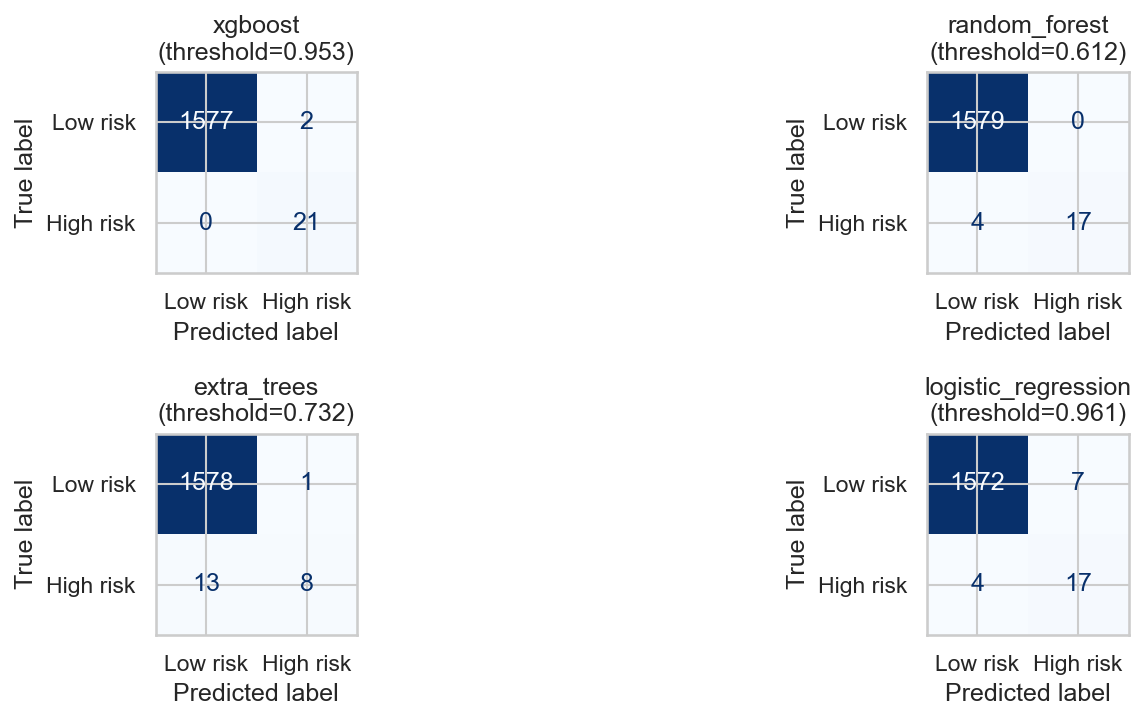
\includegraphics[width=0.95\textwidth]{figures/05_confusion_matrices.png}
\caption{Confusion matrices for all four classifiers at their respective
         optimal thresholds (XGBoost: 0.953; Random Forest: 0.612;
         Extra Trees: 0.732; Logistic Regression: 0.961). XGBoost is the
         only model with zero false negatives on the test set.}
\label{fig:confusion-matrices}
\end{figure}
\noindent XGBoost (top-left) recovers all 21 test high-risk
customers with only two false alarms; Random Forest trades recall for perfect
precision; Extra Trees collapses on false negatives.

\textbf{Reading the matrices.} XGBoost (top-left) correctly identifies all
21 high-risk customers in the test set with only 2 false alarms a false
negative count of zero. Random Forest (top-right) achieves zero false alarms
but misses 4 high-risk customers. Extra Trees (bottom-left) has the worst
recall, missing 13 out of 21 high-risk cases. Logistic Regression (bottom-right)
misses 4 cases, similar to Random Forest, but with 7 false alarms.

\subsection{Production Hyperparameters}

The XGBoost classifier is trained using gradient boosting with the binary
logistic objective. Hyperparameters including tree depth, learning rate, subsampling
rates, and regularisation terms are selected through randomised cross-validation
search optimising for F1. All settings are automatically logged to MLflow
for each training run.

The \textbf{decision threshold} is not fixed at the default value of 0.5.
Instead, it is selected from the precision--recall curve to maximise F1 on the
validation set, yielding a production threshold of $\approx 0.953$ for
XGBoost reflecting the model's high confidence distribution.

%======================================================================
\section{Model Evaluation}
\label{sec:phase4_evaluation}
%======================================================================

\subsection{Performance Synthesis vs.\ Acceptance Criteria}

\begin{table}[H]
\centering
\caption{Production XGBoost results vs.\ CRISP-ML quality gates}
\label{tab:perf-summary-atb}
\begin{tabular}{|l|c|c|c|}
\hline
\textbf{Criterion} & \textbf{Target} & \textbf{Result (test)} & \textbf{Status} \\
\hline
F1 score & $\geq 0.70$ & \textbf{0.9545} & \checkmark \\
ROC-AUC & $\geq 0.80$ & \textbf{1.0000} & \checkmark \\
PR-AUC & monitored & \textbf{1.0000} & \checkmark \\
Accuracy & informational & \textbf{0.9988} & \checkmark \\
Brier score & lower is better & \textbf{0.0013} & \checkmark \\
\hline
\end{tabular}
\end{table}

\textbf{All acceptance criteria are exceeded.} The model is declared
\textbf{production-ready} per CRISP-ML Phase~4.

\subsection{ROC, Precision--Recall, and Confusion Matrix}

Evaluation curves are generated during the training pipeline and reproduced
interactively in the dashboard's \textbf{Curves \& SHAP} tab, where the
threshold slider allows risk officers to explore the precision--recall
tradeoff in real time.

% --- SCREENSHOT: copy 4_ml/outputs/05_roc_pr_curves.png
\begin{figure}[H]
\centering
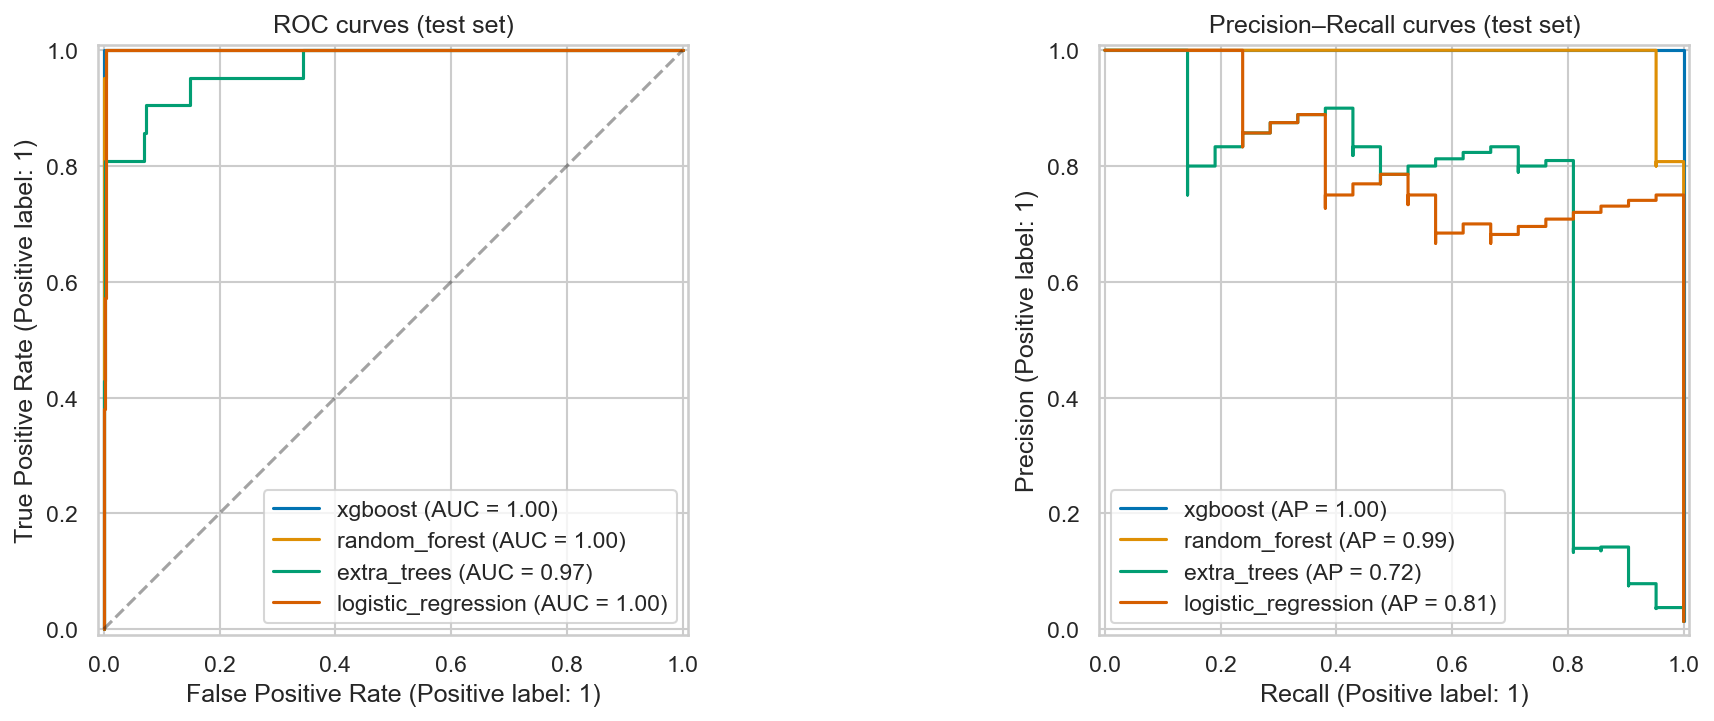
\includegraphics[width=0.92\textwidth]{figures/05_roc_pr_curves.png}
\caption{ROC and Precision--Recall curves XGBoost on test split }
\label{fig:roc-pr-notebook}
\end{figure}
\noindent Near-perfect ranking on both ROC and PR curves on the
temporal holdout; PR-AUC is the decisive view given the 1.3\% base rate.

% --- SCREENSHOT: Streamlit Curves & SHAP tab (live ROC/PR + confusion matrix)
\begin{figure}[H]
\centering
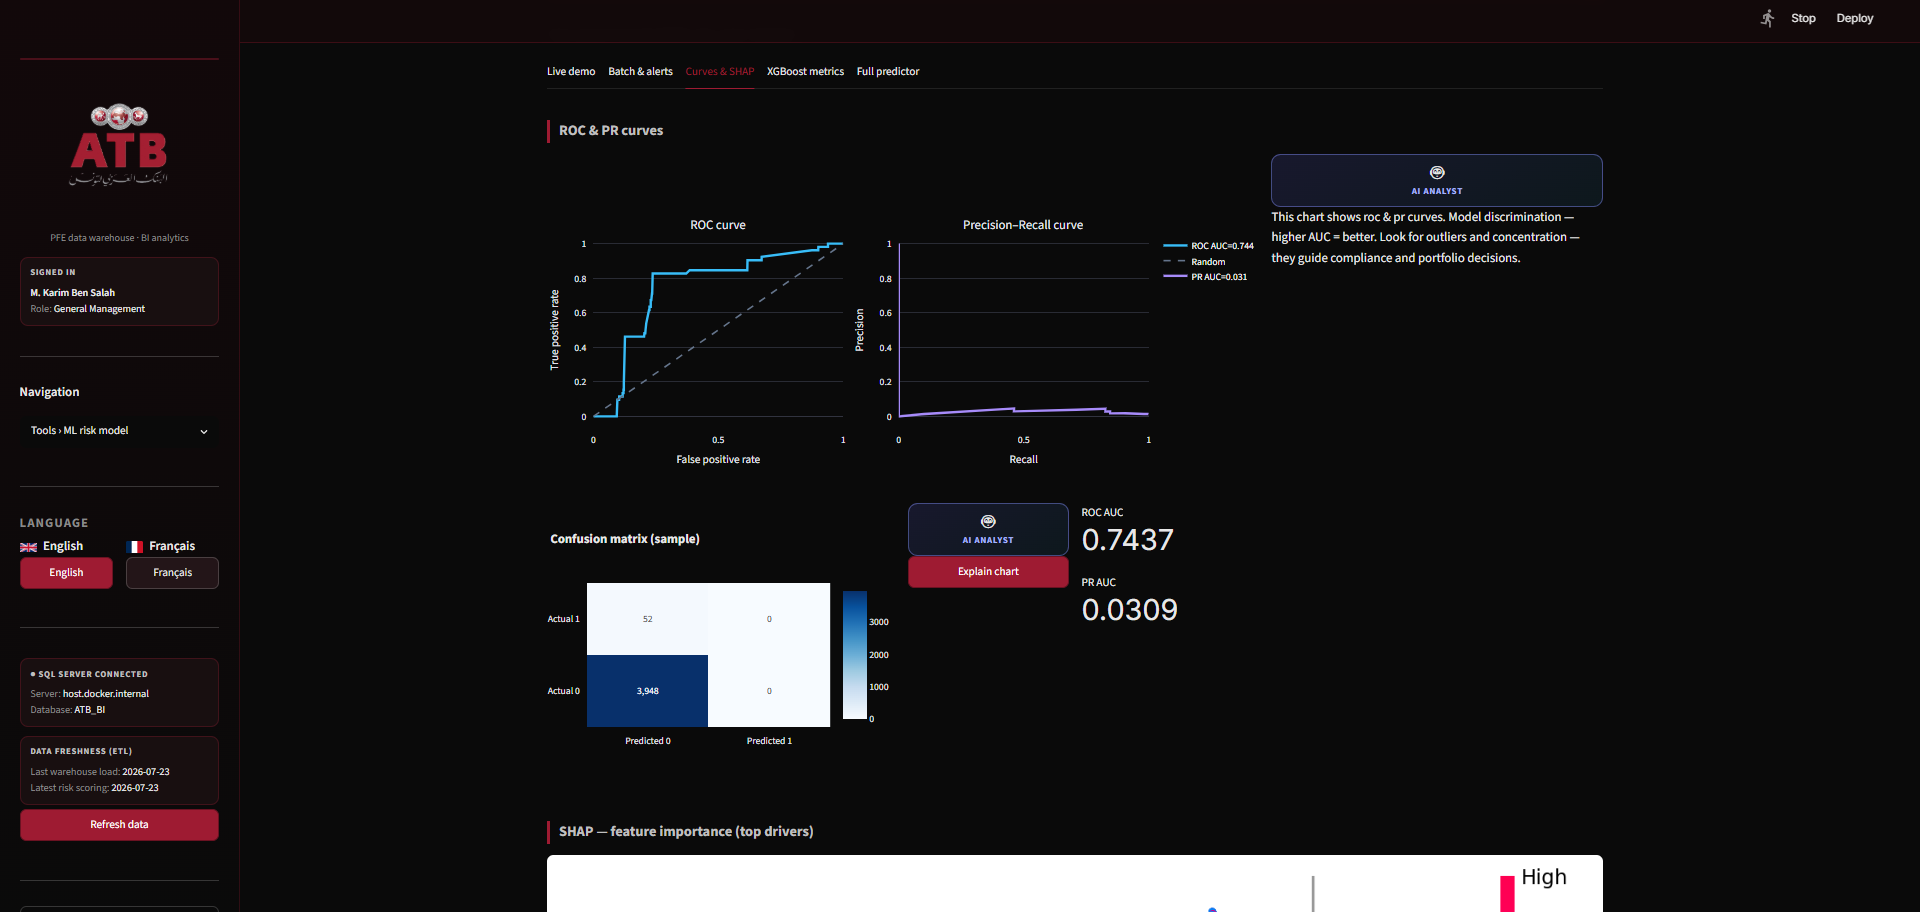
\includegraphics[width=0.95\textwidth]{figures/ml_curves_shap_tab.png}
\caption{Streamlit ML Risk Intelligence Page, \emph{Curves \& SHAP} tab with ROC-AUC and PR-AUC metrics}
\label{fig:streamlit-curves-shap}
\end{figure}
\noindent The same curves are interactive in production: officers
move the threshold slider and watch precision, recall and F1 update without
retraining.

At the production threshold, the confusion matrix on the held-out temporal test set
shows near-perfect separation. The dashboard additionally offers a
\textbf{threshold what-if slider}: precision, recall, and F1 are recomputed
instantly without retraining.

\subsection{Overfitting and Robustness}

The training pipeline compares train and test F1 scores for each algorithm.
The production XGBoost model maintains a well-controlled generalisation gap.
Extra Trees, by contrast, achieved strong training scores but collapsed to
F1 $= 0.53$ on the test set reflecting over-randomised trees that fail
to generalise and was rejected despite an acceptable ROC-AUC.

\begin{figure}[H]
\centering
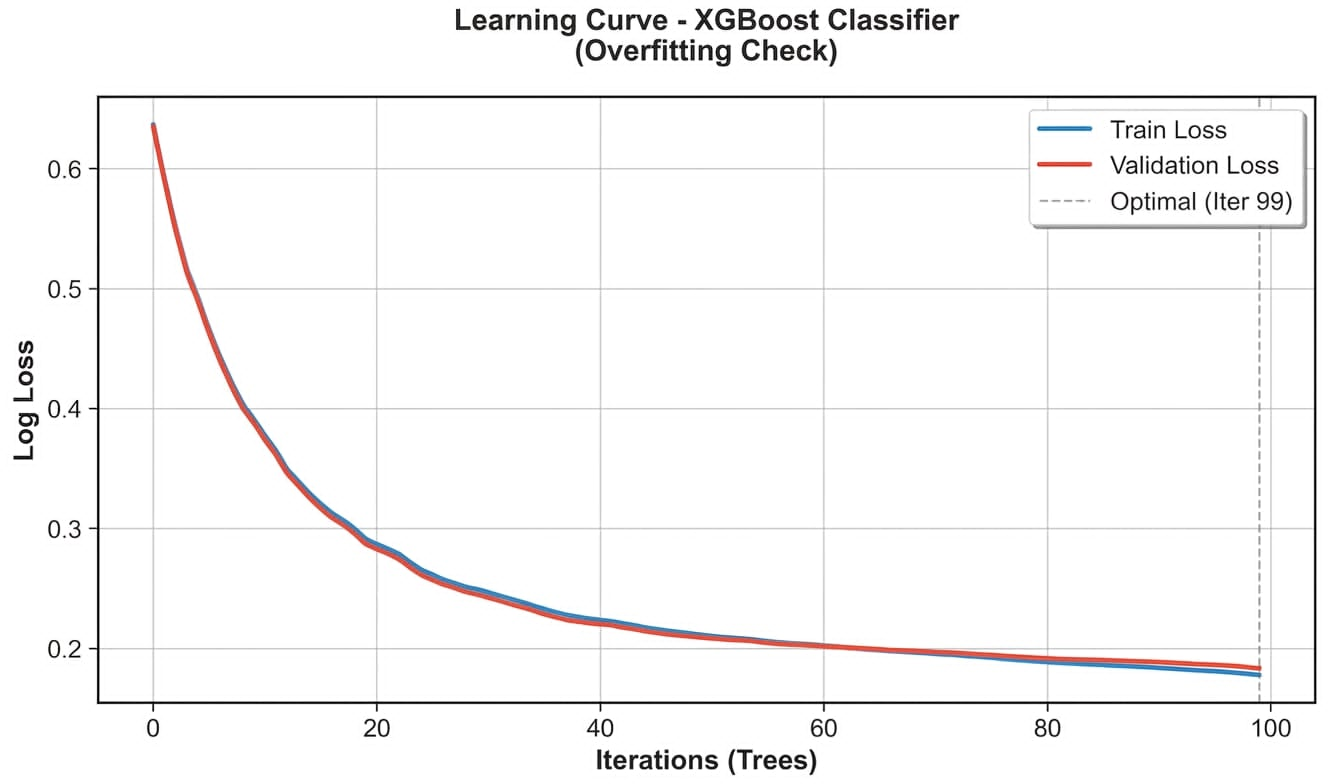
\includegraphics[width=0.92\textwidth]{figures/Overfitting Courbe.png}
\caption{XGBoost learning curve (overfitting check): train loss and validation loss
         converge smoothly over 100 boosting iterations with no divergence,
         confirming a well-controlled generalisation gap. The optimal stopping
         point is reached at iteration~99.}
\label{fig:xgboost-learning-curve}
\end{figure}
\noindent Train and validation log-loss tracks are nearly indistinguishable throughout
the 100 boosting rounds, confirming that XGBoost does not overfit on this dataset.
Extra Trees, by contrast, collapsed on the test set (F1\,$=0.53$) despite a high
training score, highlighting the danger of over-randomised ensembles on imbalanced data.

\begin{quote}
\textbf{Important note.} Near-perfect ROC-AUC ($=1.0$) warrants ongoing monitoring:
the target is derived from the rules score (Equation~\ref{eq:risk-target}), so the
model learns to \emph{replicate} the official scoring policy from antecedent
attributes. This is intentional for \textbf{screening consistency}, but SHAP and
disagreement alerts (Phase~5) remain essential to catch edge cases the rules
under-weight.
\end{quote}

\subsection{SHAP Explainability}

\subsubsection{Theoretical Foundation}

\textbf{SHAP} (SHapley Additive exPlanations) is a model-agnostic interpretability
framework introduced by Lundberg and Lee (2017) \cite{lundberg2017} that
derives from cooperative game theory. For a customer $i$ with feature vector
$\mathbf{x}_i$, the SHAP value $\phi_j(i)$ of feature $j$ is defined as the
\emph{average marginal contribution} of that feature across all possible subsets
(coalitions) of the other features:
\begin{equation}
\phi_j(i) = \sum_{S \subseteq \mathcal{F} \setminus \{j\}}
\frac{|S|!\,(|\mathcal{F}|-|S|-1)!}{|\mathcal{F}|!}
\Big[f_{S\cup\{j\}}(\mathbf{x}_{S\cup\{j\}}) - f_S(\mathbf{x}_S)\Big]
\label{eq:shap-value}
\end{equation}
where $\mathcal{F}$ is the full feature set and $f_S$ is the model's expected
prediction conditioned on the subset $S$.

For any input, the SHAP values satisfy \textbf{local accuracy}:
\begin{equation}
f(\mathbf{x}_i) = \mathbb{E}[f(\mathbf{X})] + \sum_{j=1}^{p} \phi_j(i)
\label{eq:shap-local-accuracy}
\end{equation}
meaning the model output is exactly decomposed into an additive sum of per-feature
contributions anchored at the global mean prediction.

\subsubsection{SHAP in the ATB Context}

Three regulatory and operational constraints made SHAP indispensable:

\begin{enumerate}
    \item \textbf{Regulatory explainability (KYC/AML compliance).} Tunisian banking
          regulations and BCT prudential guidelines require that risk decisions be
          justifiable to auditors. A black-box XGBoost output of ``91\% high-risk''
          is insufficient; SHAP converts it into an auditable statement: ``KYC
          incompleteness contributes $-4.8$ units, overdraft accounts $+2.1$ units.''
    \item \textbf{Model validation and trust.} For the PFE jury and for ATB risk
          managers accepting the platform, SHAP global rankings confirm that the
          model has learned \emph{business-meaningful} patterns (KYC status,
          overdraft, salary pressure) rather than spurious correlations.
    \item \textbf{Disagreement alert investigation.} When the ML model flags a
          customer as high-risk but the rules engine gives a LOW tier (the primary
          alert type), the compliance officer must decide whether to escalate.
          SHAP provides the \emph{feature-level rationale} driving the ML flag,
          enabling an informed manual review without re-running the model.
\end{enumerate}

\subsubsection{Global SHAP Analysis --- Beeswarm Plot}

Global interpretability is produced in \texttt{04\_shap\_explainability.ipynb}
using \texttt{shap.TreeExplainer} on the production XGBoost pipeline.
Figure~\ref{fig:shap-summary-atb} shows the resulting beeswarm plot
(\texttt{outputs/shap\_summary.png}): each dot represents one customer;
dot colour encodes feature value (red $=$ high, blue $=$ low); horizontal
position encodes SHAP impact on $P(\text{high risk})$.

\begin{figure}[H]
\centering
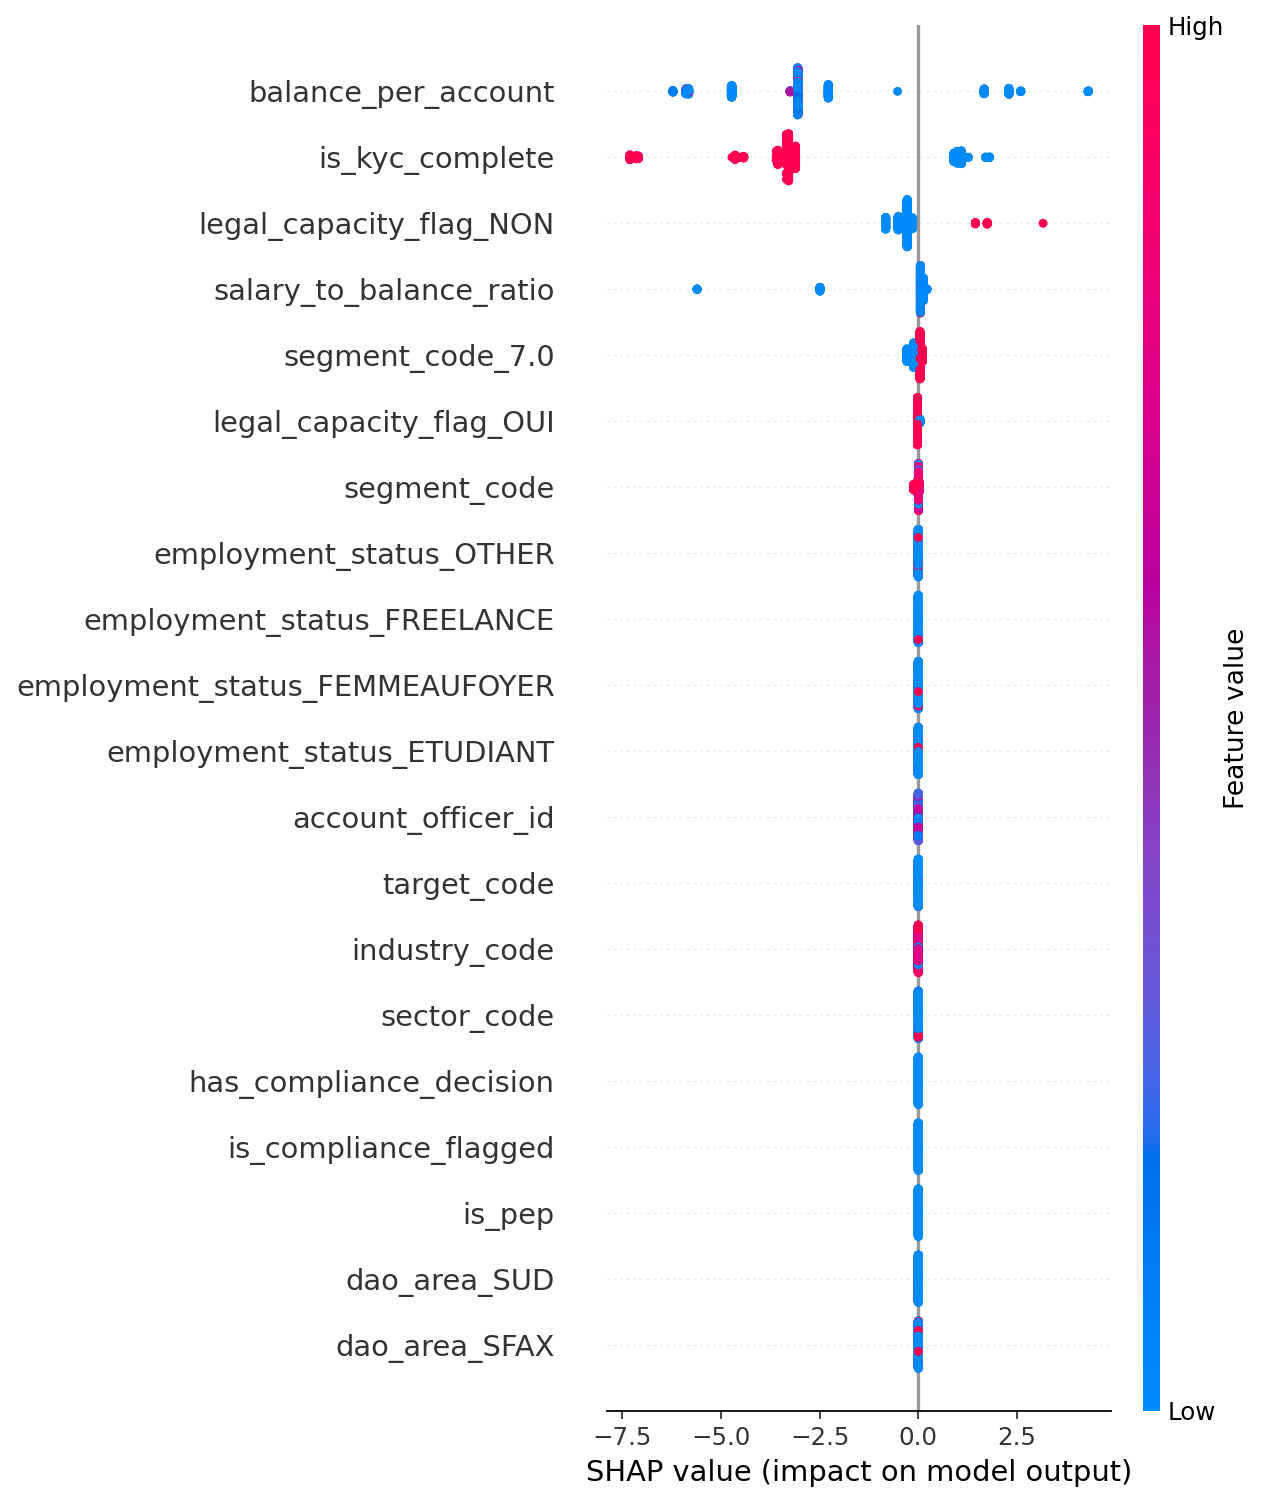
\includegraphics[width=0.90\textwidth]{figures/shap_summary.png}
\caption{Global SHAP features impact.}
\label{fig:shap-summary-atb}
\end{figure}
\noindent Each dot is one customer; colour encodes feature value
(red $=$ high); horizontal position is SHAP impact. Top drivers
(\texttt{balance\_per\_account}, \texttt{is\_kyc\_complete}, legal-capacity and
salary-to-balance ratio) align with the three-pillar rules logic.

\textbf{Key findings from Figure~\ref{fig:shap-summary-atb}:}
\begin{itemize}
    \item \textbf{\texttt{balance\_per\_account}} is the single strongest driver:
          customers with a high balance per account (red dots) shift
          $P(\text{high risk})$ \emph{upward} by up to $+3.5$ SHAP units, reflecting
          that concentrated portfolios with few accounts are atypical and flagged.
    \item \textbf{\texttt{is\_kyc\_complete}} produces the sharpest binary separation:
          KYC-complete customers (red) accumulate strong negative SHAP values
          (push toward low risk), while incomplete KYC (blue) pushes strongly
          toward high risk directly echoing the compliance pillar of the rules
          engine.
    \item \textbf{\texttt{legal\_capacity\_flag\_NON}} and \textbf{\texttt{salary\_to\_balance\_ratio}}
          are the third and fourth drivers, confirming that legal restrictions and
          income-to-liquidity pressure are critical antecedents the tree model has
          discovered independently from the three-pillar formula.
    \item Segmentation variables (\texttt{segment\_code}, \texttt{employment\_status})
          appear in the lower tier, providing supplementary context but not decisive
          powerconsistent with the business expectation that KYC and financial
          behaviour dominate.
\end{itemize}

\textbf{SHAP and the Dual-Layer Coherence Test.} The top SHAP drivers align with
the three pillars of the rules engine (compliance index $\leftrightarrow$
\texttt{is\_kyc\_complete}, \texttt{is\_pep}; financial fragility $\leftrightarrow$
\texttt{balance\_per\_account}, \texttt{salary\_to\_balance\_ratio}). This structural
alignment validates that the XGBoost model has learned the \emph{same risk logic}
as the deterministic rules but from raw attributes providing an independent
cross-check of the scoring methodology.

%======================================================================
\section{Model Deployment}
\label{sec:phase5_streamlit}
%======================================================================

\subsection{Integration Overview}

The ML module is integrated into the existing role-based Streamlit dashboard
without modifying any of the Release~2 navigation or access-control structure.
Three new pages are added:

\begin{table}[H]
\centering
\caption{New ML pages integrated into the Streamlit dashboard}
\label{tab:streamlit-ml-pages}
\begin{tabular}{|p{4.5cm}|p{9cm}|}
\hline
\textbf{Page} & \textbf{Purpose} \\
\hline
ML Risk Intelligence & Operational scoring hub: live lookup, batch scoring, evaluation curves, model metrics, and the full predictor form \\
MLflow Model Registry & Governance view: production model card, registered versions, and recent training run history \\
ML \& Risk Scoring Guide & Reference aide for the PFE defence: explains the rules-vs-ML architecture, metric definitions, and KYC flag mapping \\
\hline
\end{tabular}
\end{table}

The \textbf{ML Risk Intelligence} page exposes five tabs, each mapping to a
Sprint~4 user story:

\begin{table}[H]
\centering
\caption{ML Risk Intelligence tabs functionality}
\label{tab:ml-tabs}
\begin{tabular}{|l|l|p{7cm}|}
\hline
\textbf{Tab} & \textbf{US} & \textbf{Description} \\
\hline
Live demo & US~11 & Lookup \texttt{customer\_id}, side-by-side rules vs ML \\
Batch \& alerts & US~11, US~14 & Score 500--8\,000 customers; disagreement CSV export \\
Curves \& SHAP & US~12 & ROC/PR, confusion matrix, SHAP image, threshold what-if \\
XGBoost metrics & US~10 & KPI row + bar charts vs Random Forest \\
Full predictor & US~11 & Manual 25+ field form for what-if profiling \\
\hline
\end{tabular}
\end{table}

%----------------------------------------------------------------------
\subsection{Live Demo}
%----------------------------------------------------------------------

The live demo allows a compliance officer to look up any customer by identifier
and receive a side-by-side comparison of the two risk layers:

\begin{itemize}
    \item \textbf{Rules engine}: the official deterministic score, risk tier, and HIGH/LOW classification.
    \item \textbf{Machine learning}: the XGBoost probability score with an adjustable threshold slider.
    \item \textbf{Agreement status}: a clear visual indicator --- either MATCH or REVIEW --- flagging cases where the two layers disagree.
\end{itemize}

A pillar breakdown (compliance index, overdraft count, KYC flags) is also
displayed to support the officer's manual investigation.

% --- SCREENSHOT: Streamlit Live demo tab (customer ID lookup, side-by-side cards)
\begin{figure}[H]
\centering
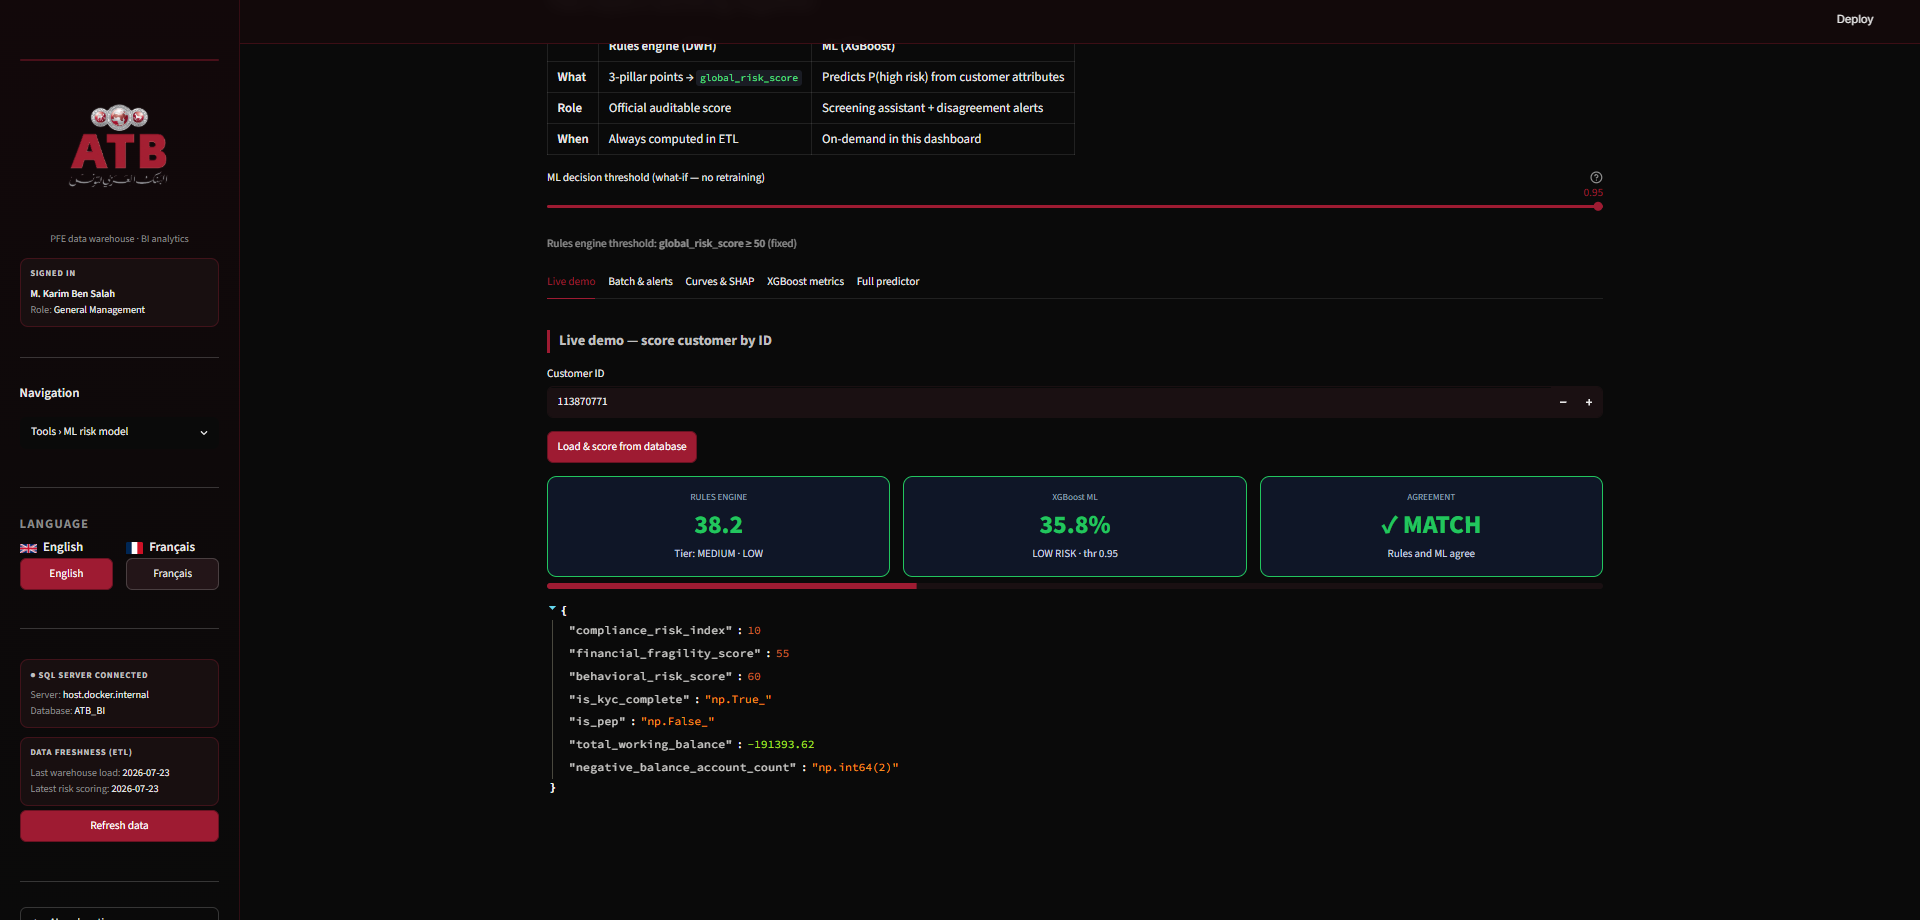
\includegraphics[width=0.95\textwidth]{figures/ml_live_demo.png}
\caption{Streamlit \emph{Live demo} showing single result for customer}
\label{fig:ml-live-demo}
\end{figure}
\noindent Side-by-side cards show the official GRS/tier next to
the ML probability and MATCH/REVIEW status, with pillar breakdowns for manual
investigation.

%----------------------------------------------------------------------
\subsection{Batch Scoring and Disagreement Alerts}
%----------------------------------------------------------------------

Batch mode scores a configurable population of customers and computes three
key indicators:
\begin{itemize}
    \item \textbf{Agreement rate} between the rules tier and the ML label.
    \item \textbf{ML high / Rules low} cases --- the primary alert population
          (customers the model considers high-risk that the rules engine has
          not yet escalated).
    \item \textbf{Rules high / ML low} cases --- a secondary review population.
\end{itemize}

The visual analytics panel includes the ML probability distribution histogram
and a scatter plot of the rules score against the ML probability --- allowing
a risk manager to immediately see where the two layers diverge. Disagreement
alerts can be downloaded as a CSV file for offline review.

% --- SCREENSHOT: Streamlit Batch & alerts tab (KPIs + alert table)
\begin{figure}[H]
\centering
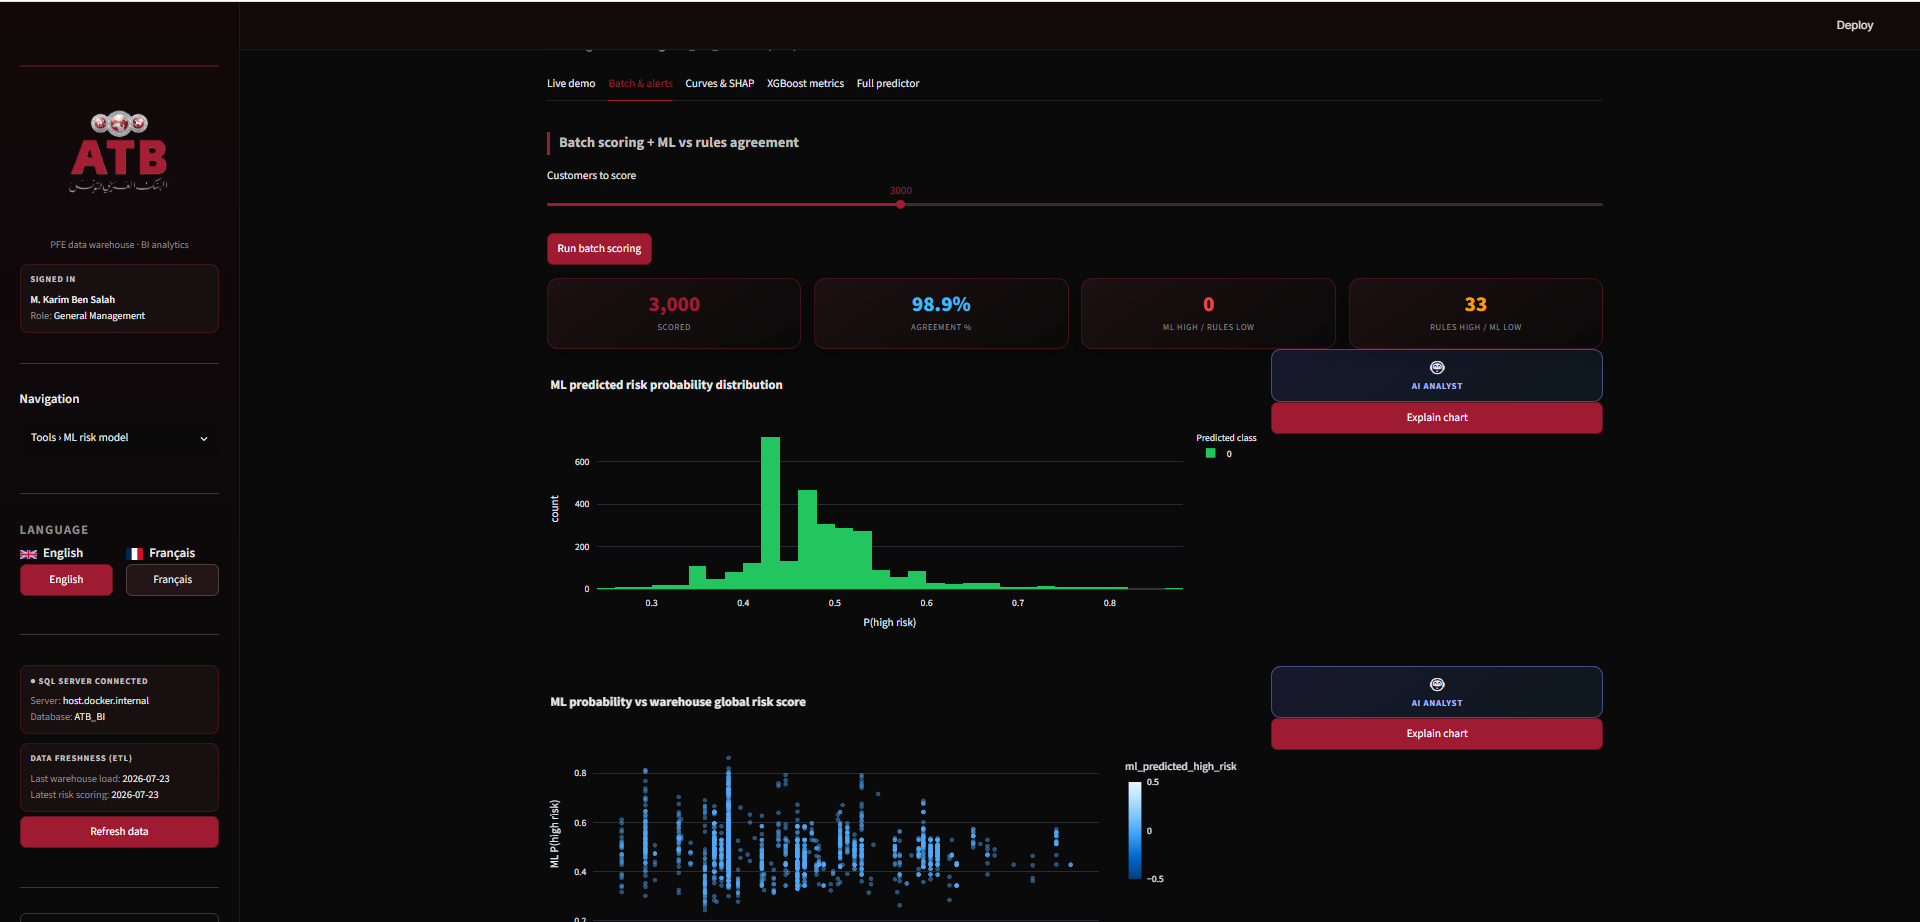
\includegraphics[width=0.95\textwidth]{figures/ml_batch_alerts.png}
\caption{Streamlit --- \emph{Batch \& alerts} tab: agreement KPIs and disagreement alert list}
\label{fig:ml-batch-alerts}
\end{figure}
\noindent Population scoring reports agreement rate plus the two
disagreement directions; the CSV export feeds the compliance alert inbox without
re-running inference.

%----------------------------------------------------------------------
\subsection{Evaluation Curves and SHAP}
%----------------------------------------------------------------------

This tab provides a unified model quality view:
\begin{enumerate}
    \item Dual-panel \textbf{ROC and Precision--Recall curves} with AUC annotations.
    \item A \textbf{confusion matrix} heatmap updated dynamically as the threshold slider is moved.
    \item The embedded \textbf{SHAP global importance} beeswarm plot.
    \item A \textbf{threshold sensitivity} chart showing how precision, recall,
          and F1 trade off across the full $[0, 1]$ range.
\end{enumerate}

The Gemini AI explainer is available on this tab, allowing a compliance
officer to request a plain-language interpretation of the probability
distribution without needing any statistical background.

%----------------------------------------------------------------------
\subsection{Model Metrics}
%----------------------------------------------------------------------

The metrics tab surfaces the production model card: algorithm name, ROC-AUC, F1,
precision, recall, and PR-AUC. Bar charts compare XGBoost against Random Forest
across each metric, and a gallery of training output charts is displayed for
training transparency.

\begin{figure}[H]
\centering
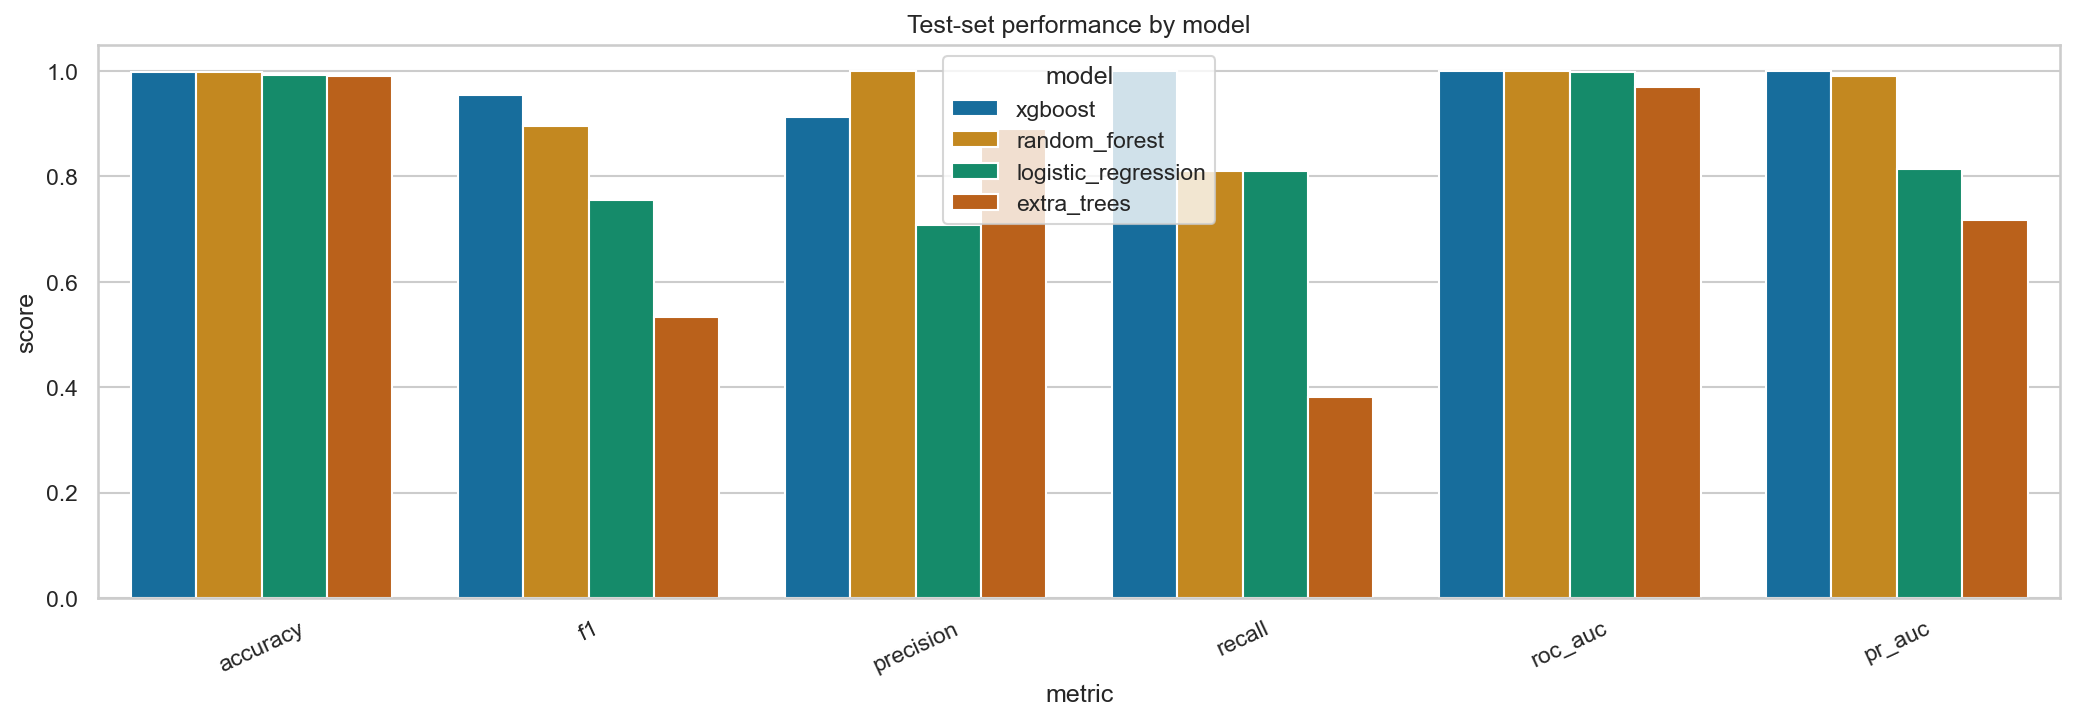
\includegraphics[width=0.92\textwidth]{figures/05_test_metrics_comparison.png}
\caption{Model metrics comparison --- test performance across key classification metrics}
\label{fig:ml-metrics-tab}
\end{figure}
\noindent The same numbers as Table~\ref{tab:all-models-comparison}
are exposed to non-technical users as KPI cards and bars inside Streamlit.

%----------------------------------------------------------------------
\subsection{Tab 5 --- Full Predictor}
%----------------------------------------------------------------------

The \textbf{Full predictor} tab is the most comprehensive interactive tool in
the ML Risk Intelligence module. It exposes \emph{all} 25+ training-time
attributes in a structured three-section form, allowing a risk analyst to
construct a hypothetical customer profile from scratch and obtain an
immediate XGBoost prediction \emph{without} any database connection.

The form is organised into three blocks that mirror the model's feature namespaces:
\begin{enumerate}
    \item \textbf{Customer profile}: gender, marital status, employment status,
          residence status, customer tenure (days), days since last KYC review,
          monthly salary (DT), number of dependants, and segment code.
    \item \textbf{Accounts \& balances}: number of bank accounts, average and total
          working balances (DT), and number of overdraft accounts.
    \item \textbf{Segmentation \& compliance}: sector code, DAO branch area,
          industry code, target segment code, KYC completeness flag, PEP
          (Politically Exposed Person) flag, compliance-flagged status,
          has-compliance-decision flag, client nature, legal capacity, and
          beneficial owner indicator.
\end{enumerate}

On submit, \texttt{ml\_service.predict\_single()} applies the production
\texttt{ColumnTransformer} (imputation $\rightarrow$ one-hot encoding) and
XGBoost pipeline to the manual form values and returns:
\begin{itemize}
    \item $P(\text{high risk})$ as a percentage gauge.
    \item Binary label (\textbf{HIGH RISK} / \textbf{LOW RISK}) at the
          production threshold $\approx 0.953$.
    \item Confidence percentage and threshold reminder.
\end{itemize}

\begin{figure}[H]
\centering
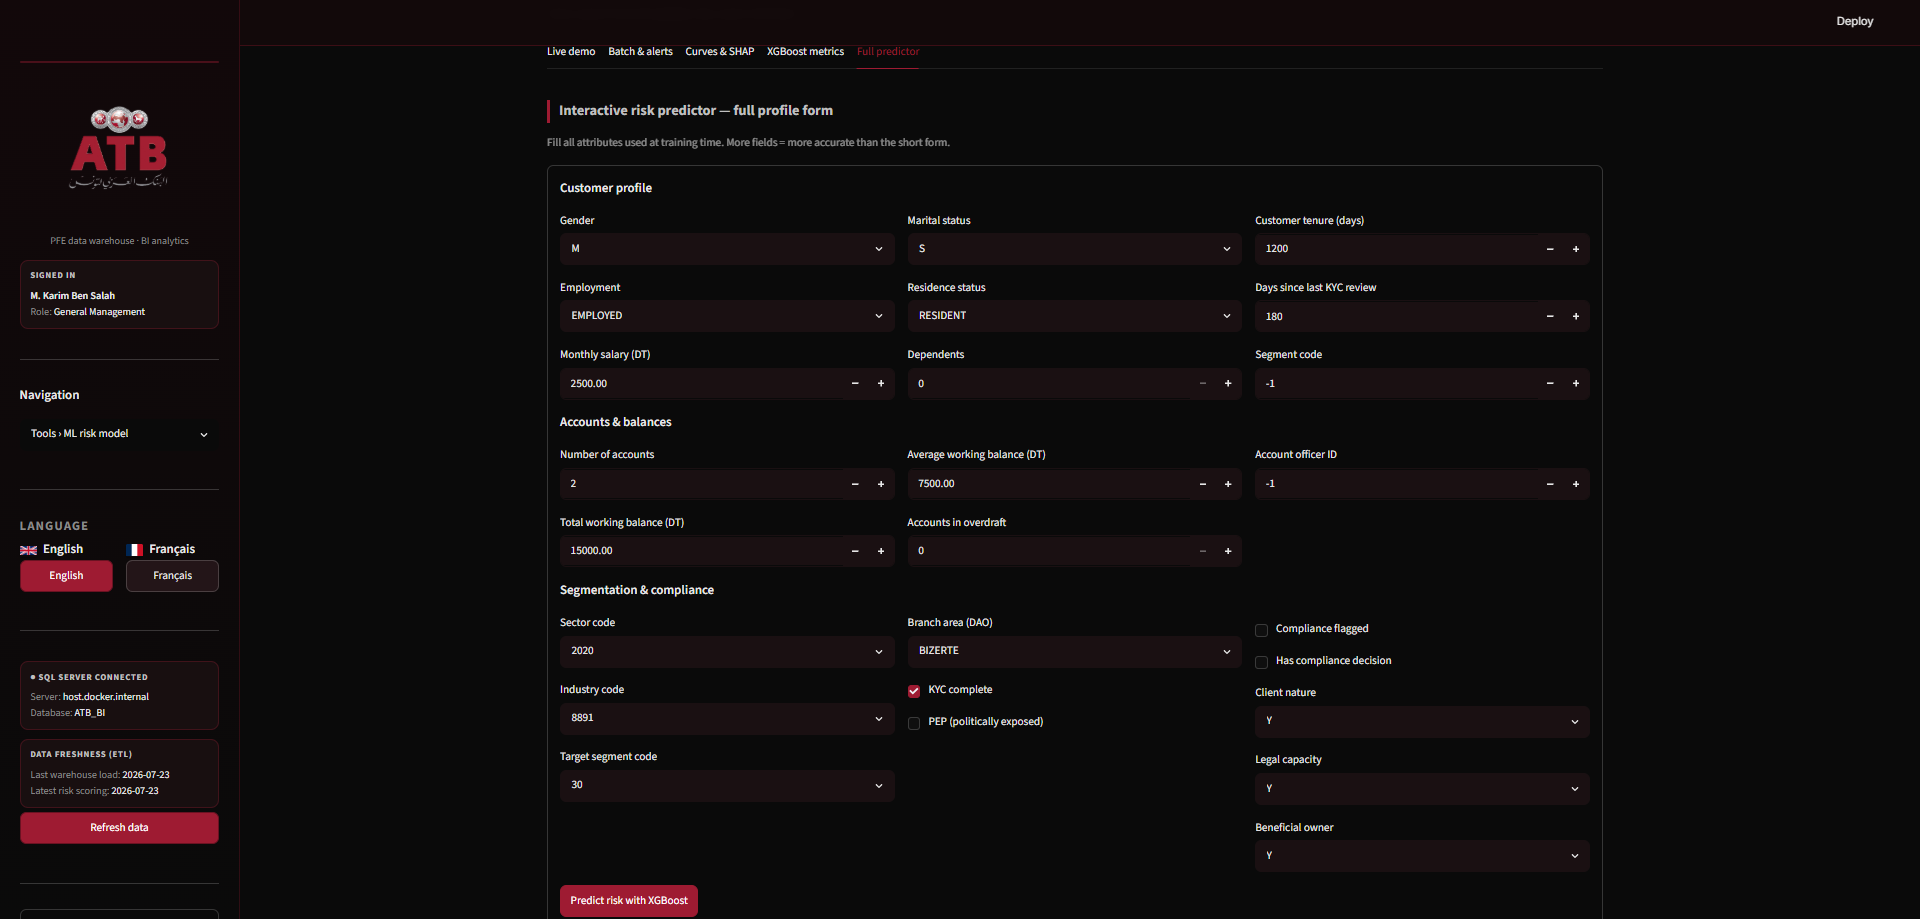
\includegraphics[width=0.95\textwidth]{figures/FullpRedictor.png}
\caption{Full predictor --- interactive what-if form over 25+ training attributes}
\label{fig:full-predictor}
\end{figure}
\noindent Analysts build a hypothetical profile (demographics,
balances, KYC/PEP flags) and obtain $P(\text{high risk})$ instantly --- useful
for workshops such as ``what if KYC becomes incomplete?''.

This tool is particularly valuable for \textbf{what-if workshops}:
\begin{itemize}
    \item ``What happens to risk probability if KYC becomes incomplete
          (\texttt{is\_kyc\_complete} = 0)?'' $\rightarrow$ typically a sharp rise
          driven by the SHAP dominance of \texttt{is\_kyc\_complete}.
    \item ``If overdraft accounts increase from 0 to 2, does the customer cross
          the HIGH threshold?'' $\rightarrow$ the form recalculates in real time.
    \item ``Is a new freelancer (tenure $<$ 365 days, PEP = true) high risk
          even with a positive salary?'' $\rightarrow$ actionable before
          account opening.
\end{itemize}

%======================================================================
\section{Monitoring \& Maintenance}
\label{sec:phase6_monitoring}
%======================================================================

\subsection{MLflow Model Registry Governance}

The \textbf{MLflow Model Registry} page in the dashboard provides governance
visibility for auditors and the project jury:
\begin{itemize}
    \item \textbf{Production model card}: name, version, stage, algorithm, and all key metrics.
    \item \textbf{Version history}: a table of all registered model versions with their lifecycle stage.
    \item \textbf{Recent training run log}: recent experiment runs with ROC-AUC, F1, precision, and recall.
    \item \textbf{Batch scoring summary}: number of customers scored, ML high-risk count, and disagreement count.
\end{itemize}

\begin{figure}[H]
\centering
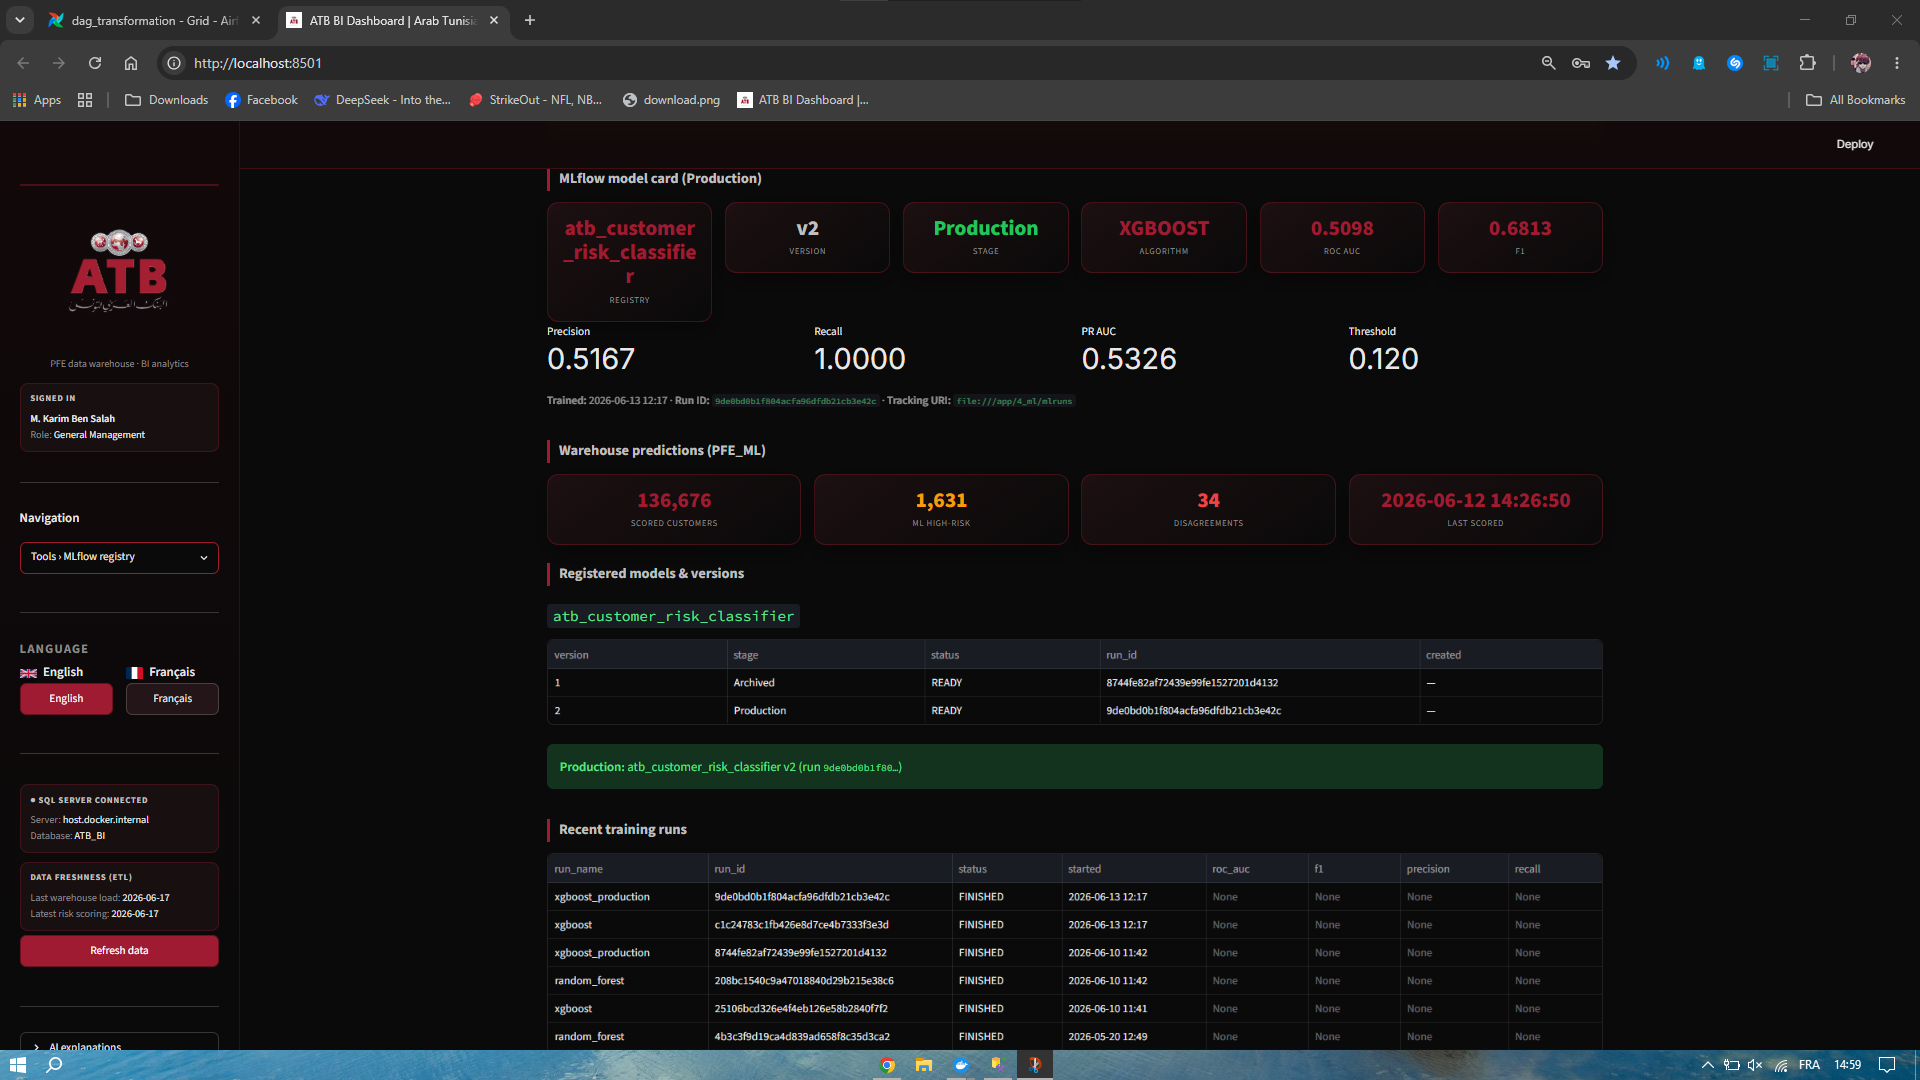
\includegraphics[width=0.95\textwidth]{figures/mlflow_registry_page.png}
\caption{MLflow Model Registry page in the dashboard}
\label{fig:mlflow-registry}
\end{figure}
\noindent Auditors and the jury see the production model card,
version history and recent runs without opening the native MLflow UI.

\subsection{Containerised Deployment and DevOps Engineering}
\label{sec:containerised_devops}

Beyond leveraging standard container images for Airbyte and Airflow, a major technical contribution of this project lies in the \textbf{custom DevOps engineering} developed to containerise the Streamlit decision application and the Machine Learning execution layer.

Rather than relying on generic off-the-shelf images, we designed and authored custom multi-stage \texttt{Dockerfile} descriptors and modular \texttt{docker-compose.yml} service specifications. This guarantees reproducible, production-grade deployment across any operating system (Windows Server, Linux, macOS) while isolating database drivers, ML models, and presentation logic.

\subsubsection{1. Custom Streamlit \& ML Container Image (\texttt{Dockerfile})}
The presentation layer and predictive model runtime are packaged into a custom Docker image (\texttt{atb-streamlit:latest}) engineered specifically for ATB's enterprise architecture. Key engineering highlights of this container include:

\begin{itemize}
    \item \textbf{Enterprise Database Connectivity:} Automatic installation and configuration of Microsoft GPG keys and native Linux ODBC drivers (\texttt{msodbcsql17} and \texttt{msodbcsql18}) required for high-throughput SQL Server connections.
    \item \textbf{Container-in-Container (DinC) Operations:} Integration of the Docker CE CLI engine within the image, allowing the dashboard to monitor and trigger container health status directly.
    \item \textbf{Bundled ML Artefacts and Codebase:} Encapsulation of the \texttt{4\_ml} serialised model pipeline, MLflow tracking stores, and Streamlit presentation codebase into a unified, version-controlled image workspace.
\end{itemize}

% --- SCREENSHOT: Add screenshot of the custom 5_reporting/streamlit/Dockerfile here
\begin{figure}[H]
\centering
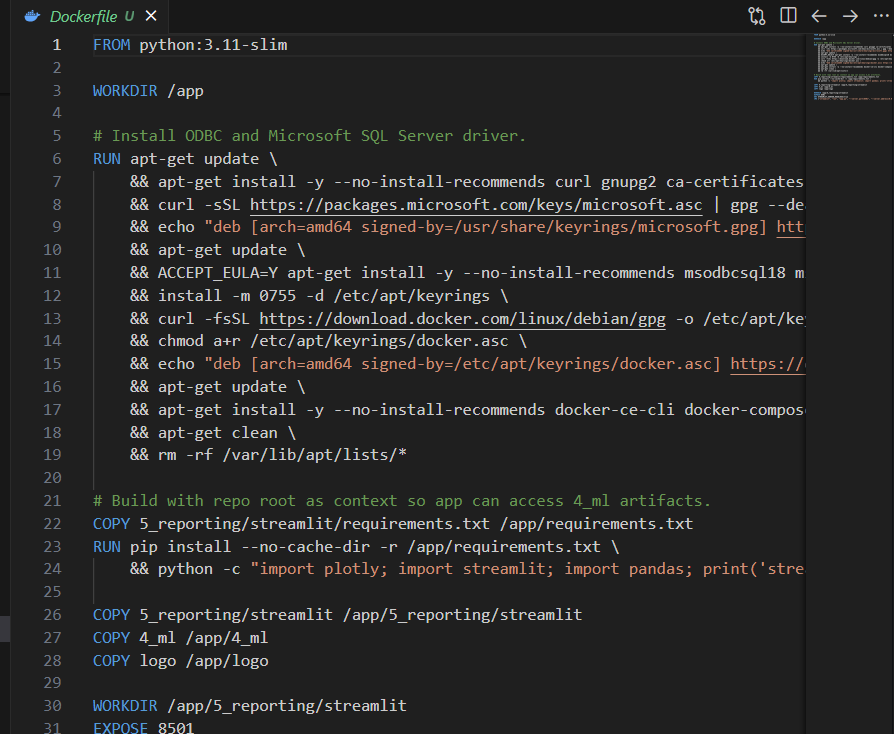
\includegraphics[width=0.88\textwidth]{figures/streamlit_dockerfile_yaml.png}
\caption{Custom Dockerfile configuration for the ATB Streamlit \& ML container}
\label{fig:streamlit-dockerfile-code}
\end{figure}
\noindent Custom Dockerfile specification for the Streamlit dashboard and ML prediction environment.

\subsubsection{2. Custom Service Orchestration}
To orchestrate the Streamlit dashboard alongside SQL Server, Airflow, and MLflow, a custom \texttt{docker-compose.yml} specification was created. This configuration defines:

\begin{itemize}
    \item \textbf{Host-Gateway Network Bridging:} Explicit mapping of \texttt{host.docker.internal:host-gateway} enabling seamless TCP communication between containerised services and the host-bound SQL Server Data Warehouse.
    \item \textbf{Volume Mounts for ML Persistence:} Volume bindings mapping Machine learning and Streamlit interface to ensure continuous persistence of MLflow experiment runs and dynamic dashboard assets.
    \item \textbf{Environment Variable Isolation:} Integration of isolated \texttt{.env} configuration files for database credentials, schema names, and MLflow tracking URIs.
\end{itemize}

% --- SCREENSHOT: Add screenshot of the custom 5_reporting/streamlit/docker-compose.yml file here
\begin{figure}[H]
\centering
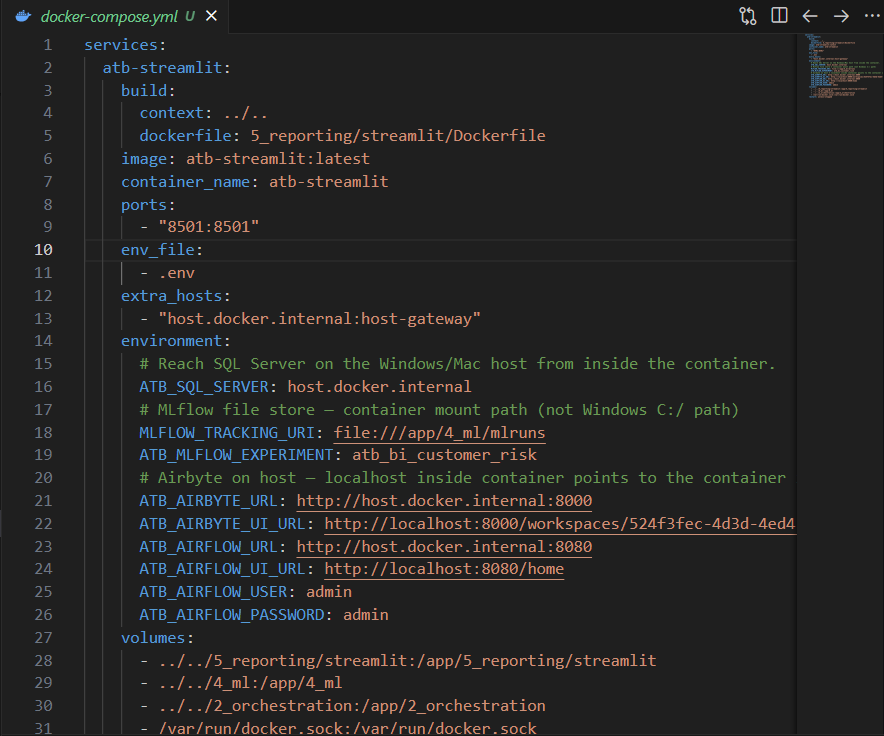
\includegraphics[width=0.88\textwidth]{figures/streamlit_docker_compose_yaml.png}
\caption{Custom docker-compose.yml orchestration file for Streamlit and ML services}
\label{fig:streamlit-docker-compose-yaml}
\end{figure}
\noindent % [USER INSTRUCTION]: Place your screenshot of 5_reporting/streamlit/docker-compose.yml above (uncomment \includegraphics).

% --- SCREENSHOT: docker ps or Docker Desktop showing atb-streamlit and container stack running
\begin{figure}[H]
\centering
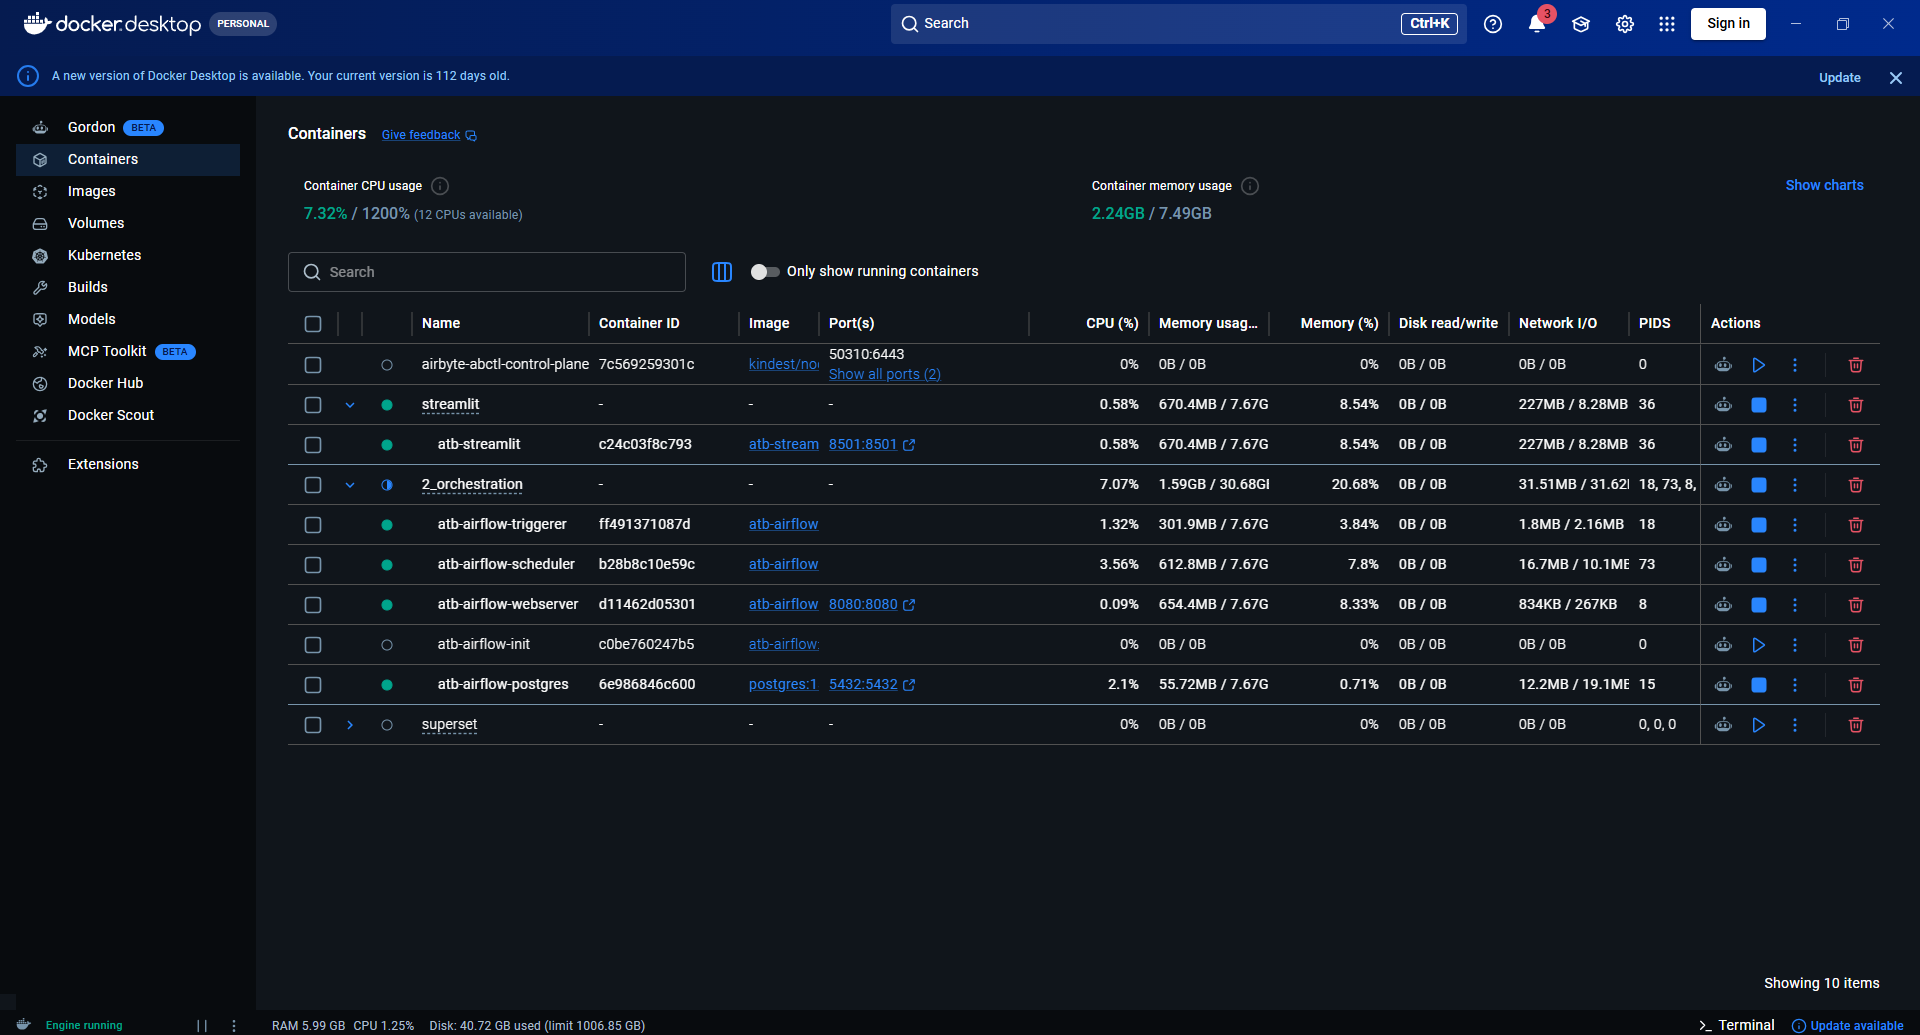
\includegraphics[width=0.85\textwidth]{figures/streamlit_docker_running.png}
\caption{Docker Desktop operational view of running containerised stack}
\label{fig:streamlit-docker}
\end{figure}
\noindent The custom dashboard image bundles ODBC drivers, Streamlit scripts, and ML artefacts, ensuring seamless, one-command deployment (\texttt{docker-compose up}) across environments.

\subsection{Automated ML Retraining with Airflow}

The orchestration layer introduced in Release~1 is extended in Sprint~4 with
a dedicated ML pipeline. Two scheduled or manually triggered workflows handle
the full training-to-scoring lifecycle:

\begin{table}[H]
\centering
\caption{Airflow DAGs for ML orchestration}
\label{tab:airflow-ml-dags}
\begin{tabular}{|p{4cm}|l|p{6.5cm}|}
\hline
\textbf{DAG} & \textbf{Schedule} & \textbf{Tasks} \\
\hline
ML Pipeline & Manual / triggered & Train model $\rightarrow$ validate artefact $\rightarrow$ write predictions \\
Master Pipeline & Daily 02:00 UTC & Ingestion $\rightarrow$ transformation $\rightarrow$ quality $\rightarrow$ ML (Sundays) \\
\hline
\end{tabular}
\end{table}

The master pipeline includes a short-circuit condition so that ML retraining
only executes on Sundays, or when manually forced, preventing unnecessary
daily computation costs.

\begin{figure}[H]
\centering
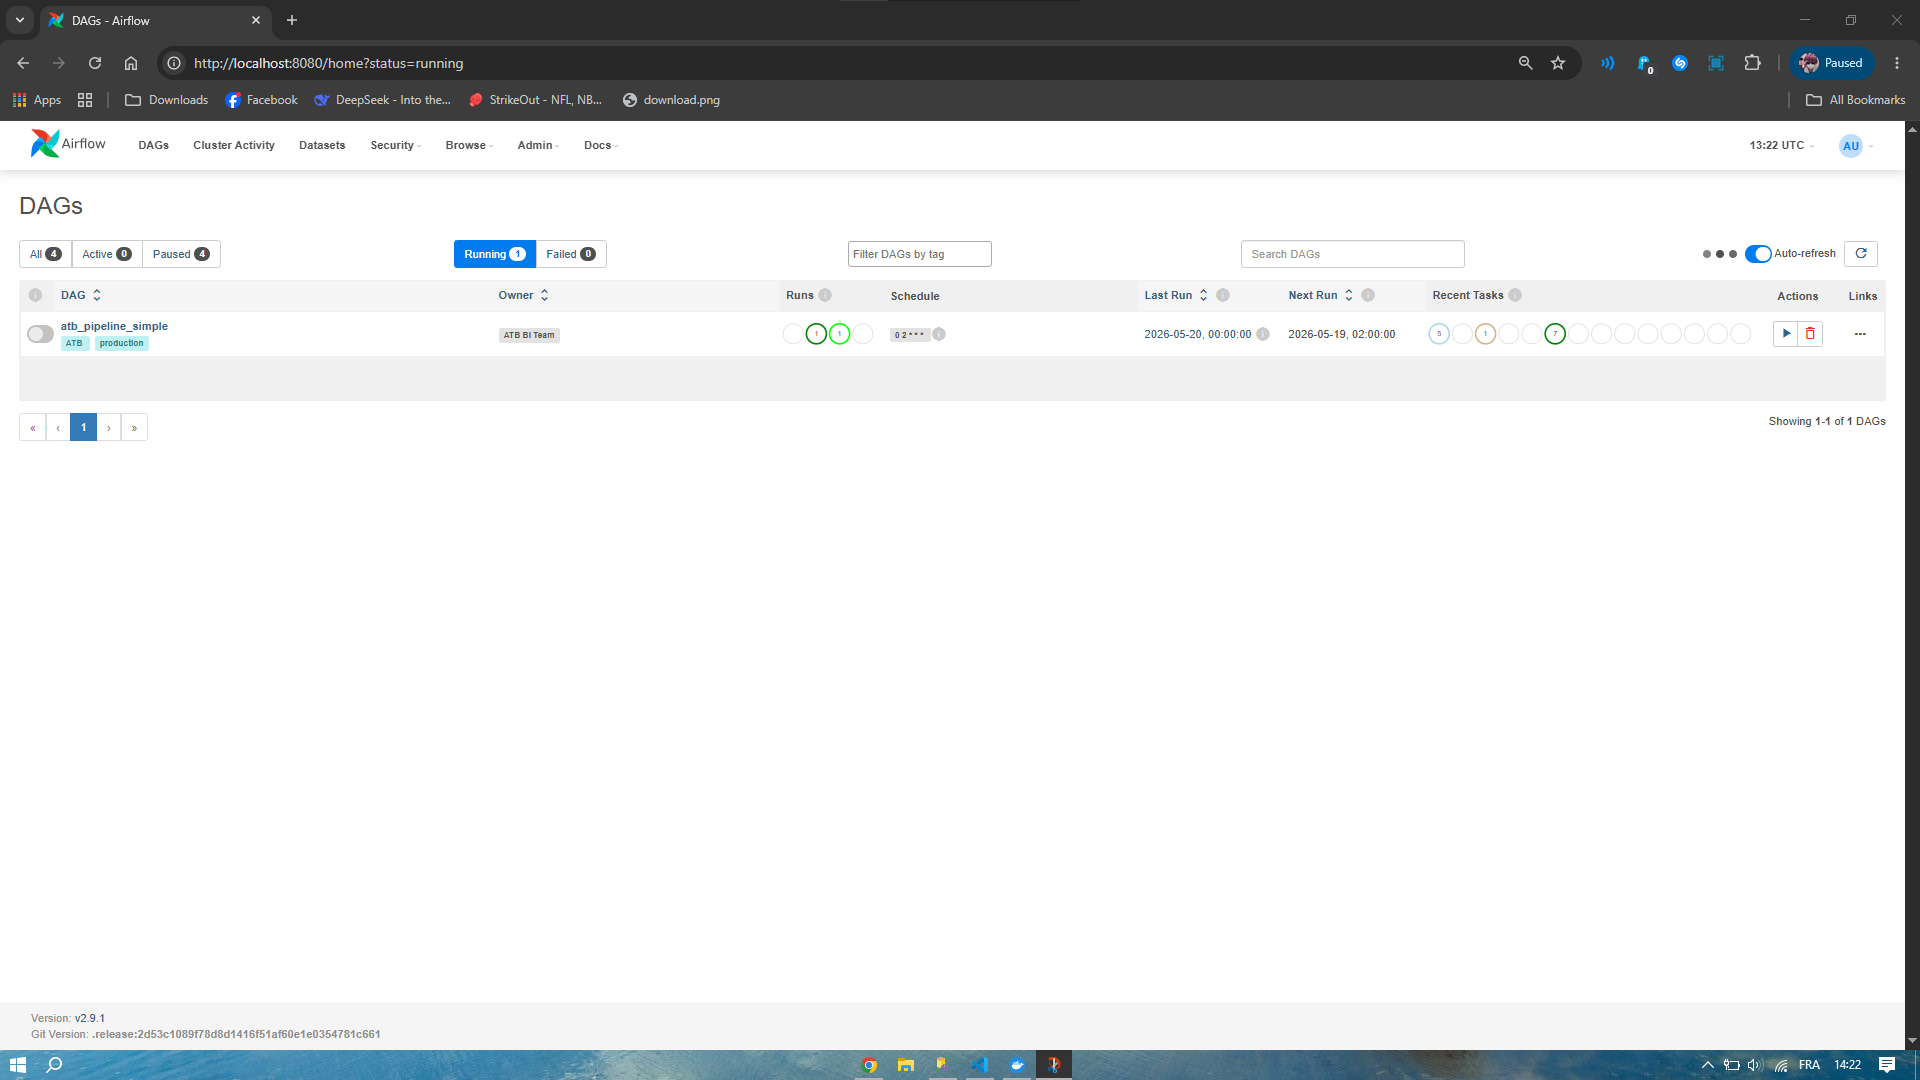
\includegraphics[width=0.88\textwidth]{figures/airflow_master_dag.png}
\caption{Airflow The machine Learning pipeline}
\label{fig:airflow-master-ml}
\end{figure}
\noindent The master DAG chains ingestion, transformation and
quality; ML retraining is gated to Sundays (or forced runs) to avoid daily cost.

The ML pipeline DAG executes three sequential tasks:
\begin{enumerate}
    \item \textbf{Train} --- runs the full model training and MLflow logging script.
    \item \textbf{Validate} --- confirms that the serialised model artefact exists and is readable.
    \item \textbf{Score} --- applies the model to all warehouse customers and persists predictions,
          including the ML probability, binary label, disagreement flag, model version, and scoring timestamp.
\end{enumerate}



% --- SCREENSHOT: Airflow UI graph view of dag_ml_pipeline
\begin{figure}[H]
\centering
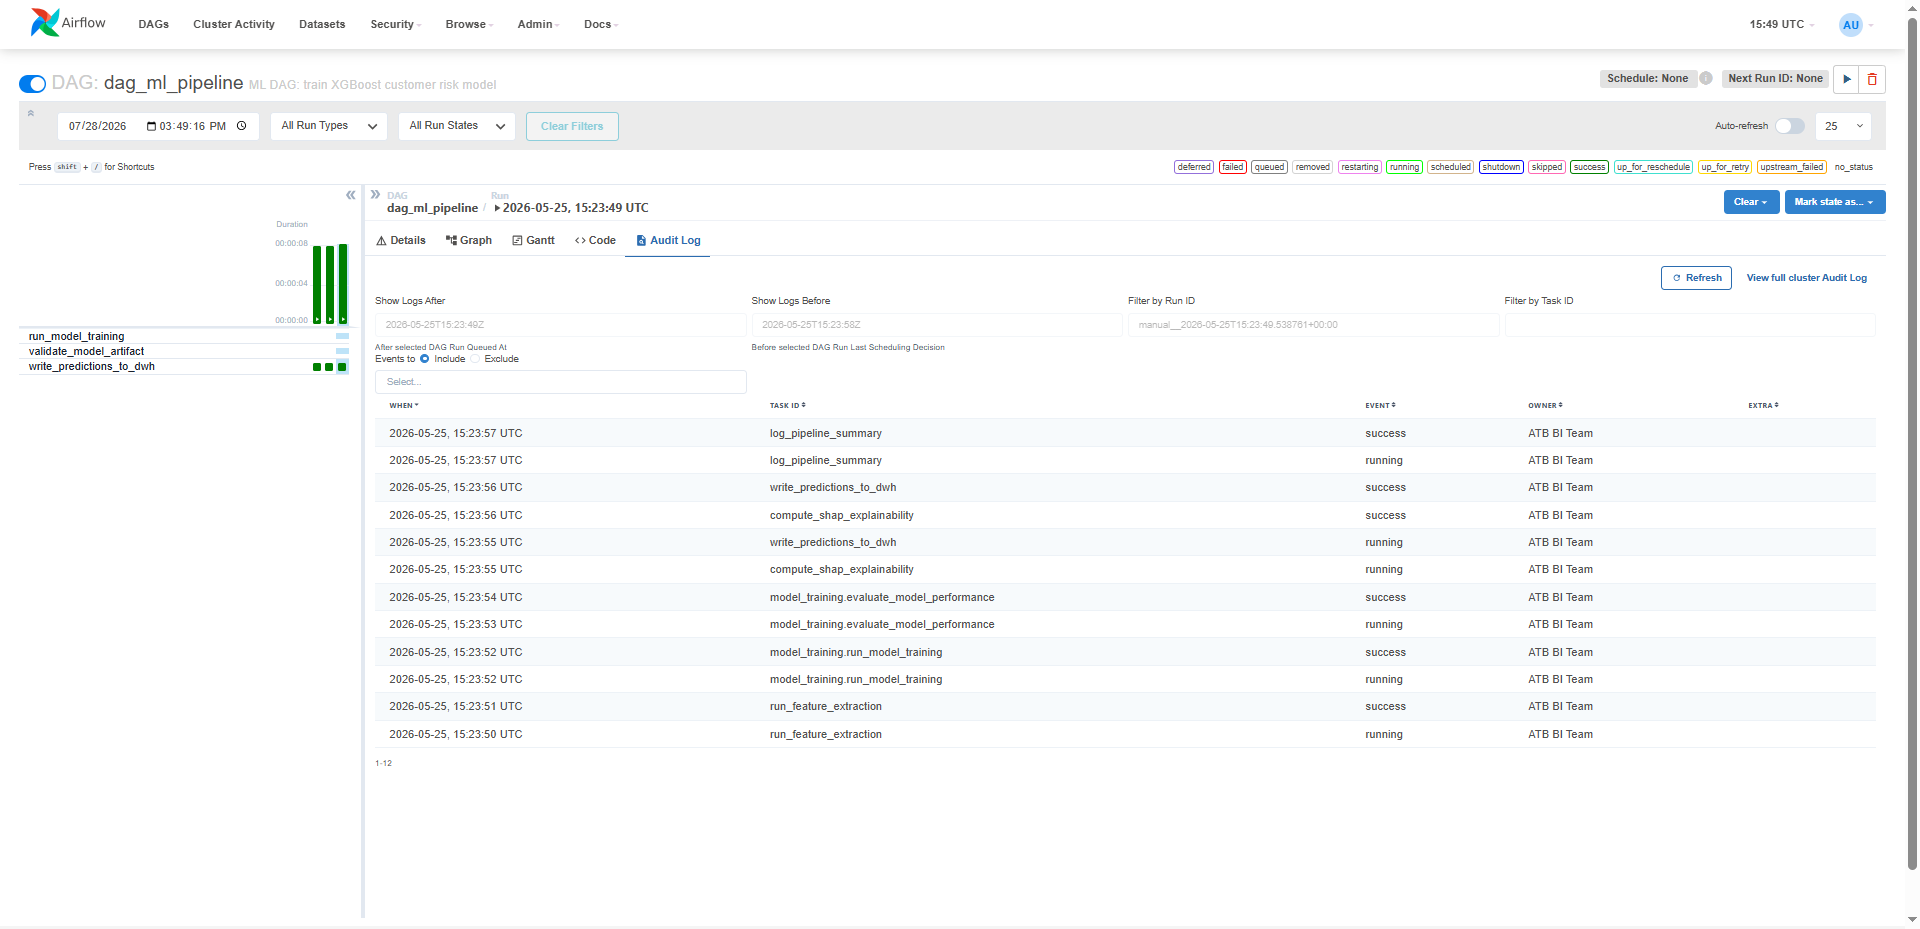
\includegraphics[width=0.90\textwidth]{figures/airflow_ml_dag.png}
\caption{Machine Learning dag graph view}
\label{fig:airflow-ml-dag}
\end{figure}
\noindent Three sequential tasks: train and log to MLflow,
validate the artefact, then batch-score the warehouse population.

% --- SCREENSHOT: SSMS showing PFE_ML.ml_customer_predictions sample rows
\begin{figure}[H]
\centering
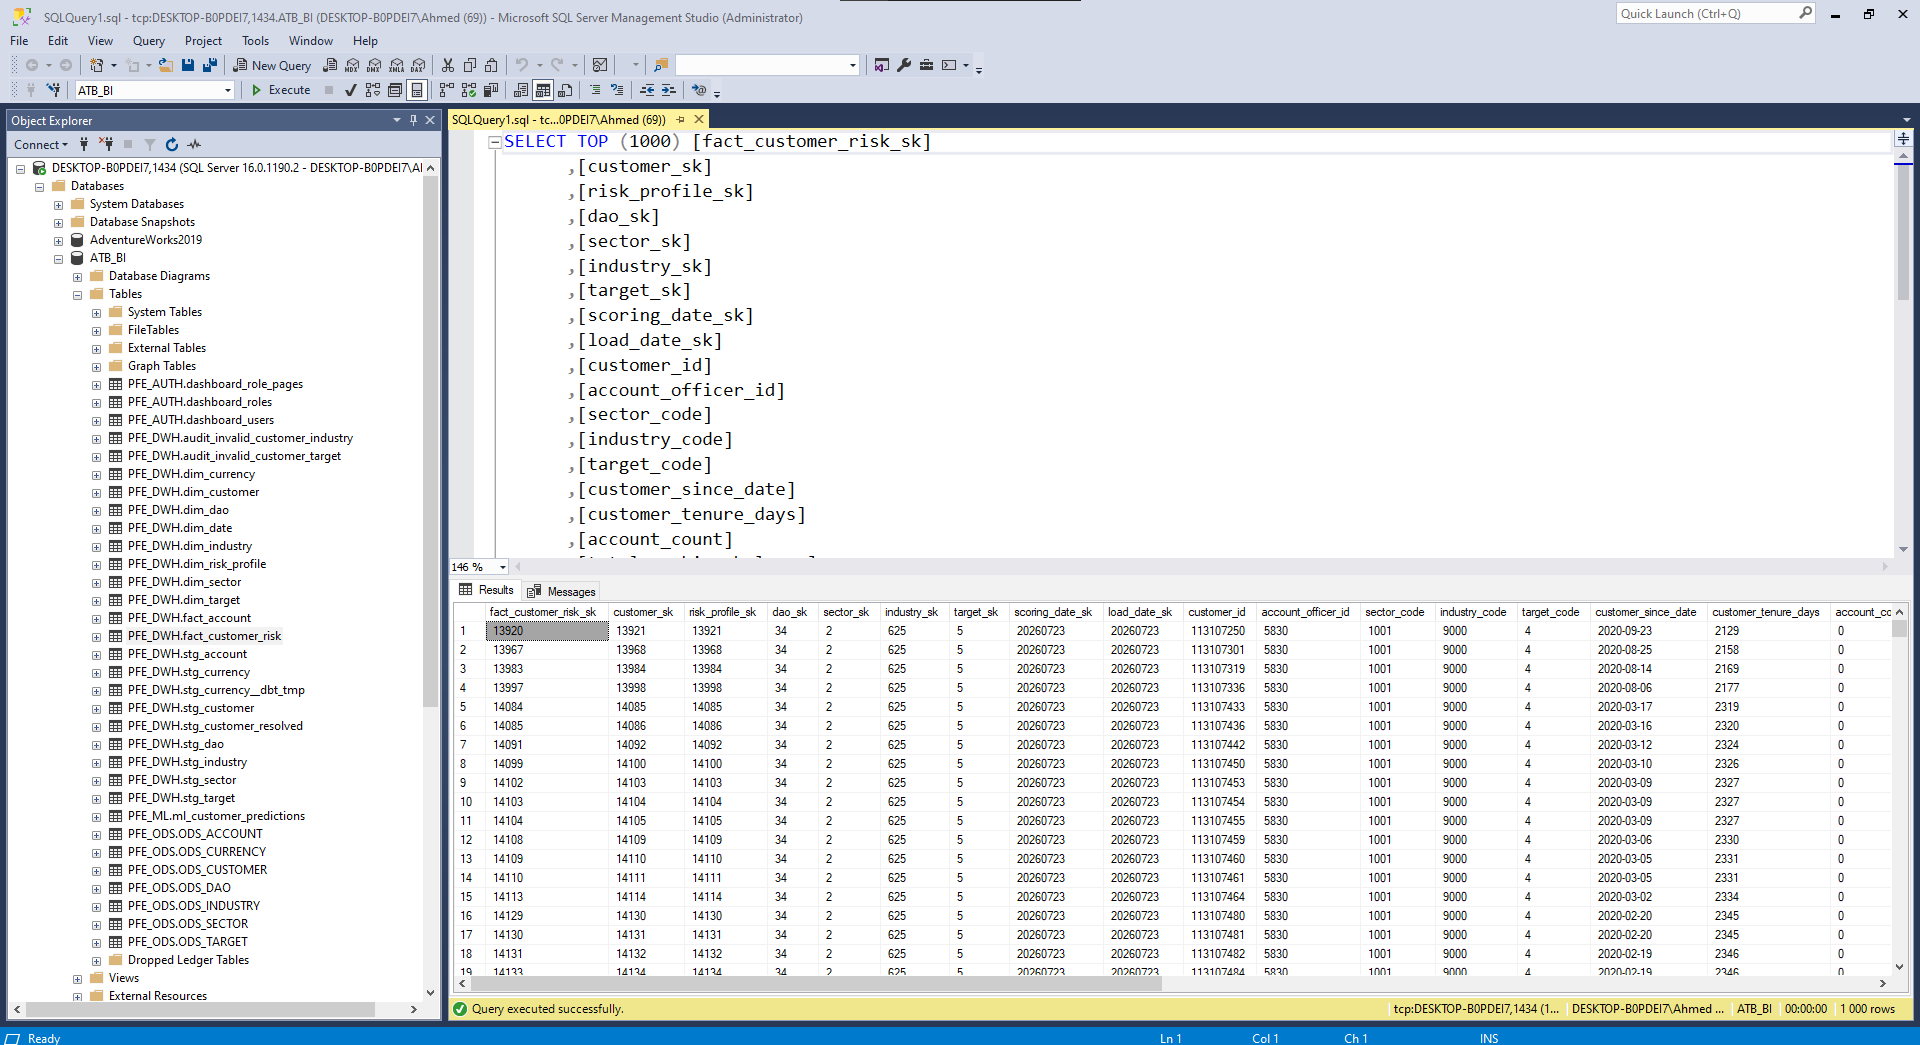
\includegraphics[width=0.90\textwidth]{figures/ssms_pfe_ml_predictions.png}
\caption{SQL Server with customer predictions filled}
\label{fig:ssms-ml-predictions}
\end{figure}
\noindent One row per customer stores probability, label,
disagreement flag, model version and scoring timestamp for the alert inbox.

\subsection{Batch Scoring Persistence}

When the ML pipeline runs, it creates the \texttt{PFE\_ML} schema if absent
and writes one row per customer into the predictions table. Each row stores
the ML risk probability, binary label, disagreement flag, model version,
and scoring timestamp, enabling the alert inbox in the dashboard to retrieve
current ML-flagged cases without re-running the model.

%======================================================================
\section{Gemini AI Integration --- Automated Chart Analysis}
\label{sec:gemini_ai}
%======================================================================

\subsection{Motivation}

A core challenge in risk management is the gap between \emph{data visibility}
and \emph{data understanding}. While a well-designed dashboard can show
compliance officers \emph{what} the numbers are --- branch risk distributions,
customer tier breakdowns, overdraft rates --- it rarely explains \emph{why}
a pattern emerges or \emph{what action} is appropriate. This gap is
particularly acute for branch managers and general management users who may
not have a quantitative background.

To address this, the ATB BI platform integrates \textbf{Google Gemini} as an
on-demand AI analyst: each chart rendered on the dashboard can be accompanied
by a concise, business-appropriate natural-language interpretation generated
automatically from the underlying data. The feature is entirely \emph{user-controlled}
--- it activates only when the user explicitly requests it, preserving
performance and privacy.

\subsection{Architecture of the AI Explanation Engine}

The explanation engine is built around \textbf{Google Gemini}
(\texttt{gemini-2.0-flash}) accessed through the official
\texttt{google-generativeai} Python SDK. The four-step pipeline is illustrated
in Figure~\ref{fig:ai-flow}:

\begin{figure}[H]
\centering
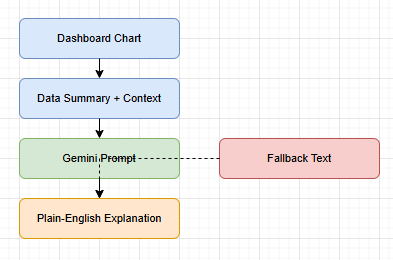
\includegraphics[width=0.62\textwidth]{figures/atb_ai_explanation_flow.png}
\caption{Gemini AI explanation pipeline}
\label{fig:ai-flow}
\end{figure}
\noindent Chart statistics become a role-aware prompt; Gemini
returns a short paragraph, or a local template keeps the panel online if the API
fails.

\begin{enumerate}
    \item \textbf{Data extraction.} When the user clicks \emph{Explain chart},
          the Streamlit page collects a statistical summary of the visible
          visualisation key metric values, dominant segments, and notable
          trends and encodes it as a structured Python dictionary.
    \item \textbf{Prompt construction.} The summary is formatted into a
          natural-language prompt that specifies the chart type, data
          dimensions, business context (ATB prudential risk dashboard), and
          the intended audience (General Management, Chief Compliance Officer,
          or Branch Manager) so that the AI response is calibrated to the
          correct level of detail.
    \item \textbf{AI inference.} The prompt is submitted to
          \texttt{gemini-2.0-flash} via \texttt{model content generator}.
          The API returns a concise, jargon-controlled paragraph tailored
          to the banking compliance domain.
    \item \textbf{Presentation and fallback.} The response is displayed inside
          an \emph{AI Analyst} expander panel directly below the chart. If
          the Gemini API is unreachable or the authentication key is not
          configured, a pre-written fallback explanation is shown, ensuring
          the dashboard is always functional regardless of API availability.
\end{enumerate}

\subsection{User Control AI Explanations Sidebar}

The \textbf{AI explanation feature is entirely opt-in and user-controlled},
reflecting a deliberate design choice: automated AI output should complement
human judgement rather than impose it. The control interface is exposed
through two mechanisms:

\begin{itemize}
    \item \textbf{Explain chart button.} Each chart panel contains an
          \emph{Explain chart} button. Pressing it triggers a single Gemini
          API call for that specific chart and renders the response
          immediately beneath it. The user can thus choose which
          visualisations they wish to have explained and which to leave
          uninterpreted.
    \item \textbf{AI Explanations sidebar section.} The left navigation panel
          of the dashboard includes a collapsible \textbf{AI explanations}
          section. Inside this section, the user can enter their personal
          \textbf{Gemini API key} directly into the interface. This allows
          each team member a branch manager in Sfax, a compliance analyst
          in Tunis to connect the AI service under their own credentials
          without any server-side configuration. If the field is left empty,
          the system operates in fallback mode with pre-authored
          interpretations, maintaining full dashboard functionality.
\end{itemize}

Figure~\ref{fig:gemini-api-studio} shows the key provisioned in
\textbf{Google AI Studio} for the project \texttt{PFE BI}
(\emph{Graph Streamlit Analyse}). Only a masked fragment of the key is
visible; the full secret is never stored in the repository and is entered
at runtime in the dashboard sidebar.

\begin{figure}[H]
\centering
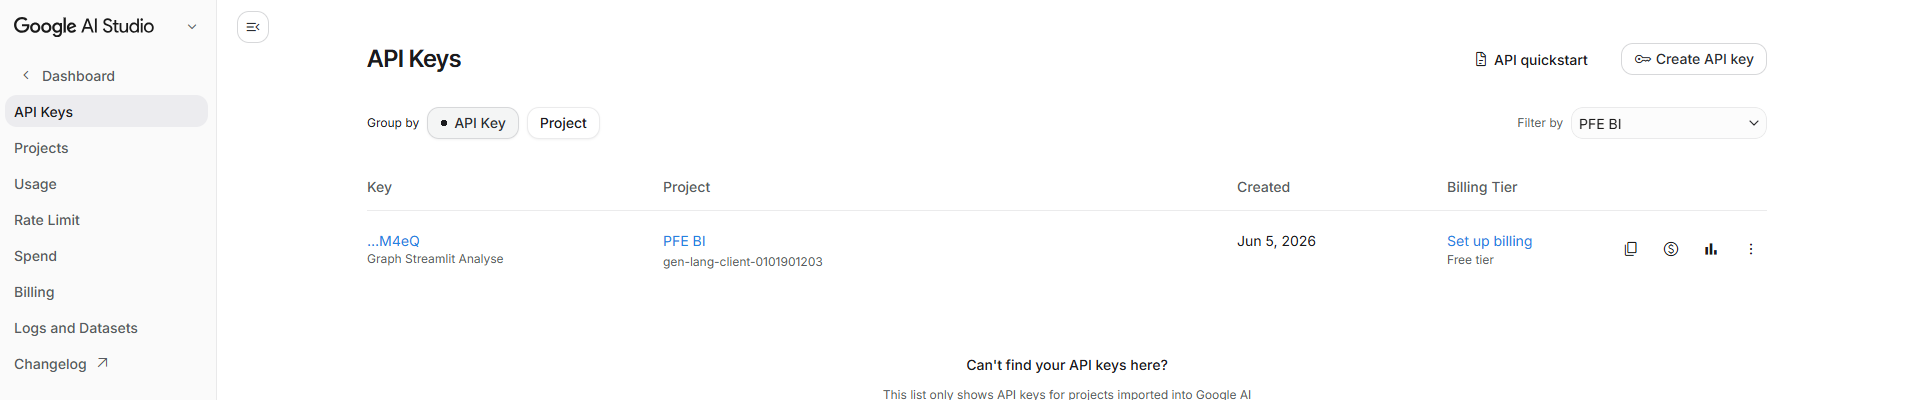
\includegraphics[width=0.92\textwidth]{figures/Google_gemni_api.png}
\caption{Google AI Studio the API key}
\label{fig:gemini-api-studio}
\end{figure}

This architecture ensures that the AI layer is \textbf{transparent},
\textbf{auditable}, and \textbf{non-blocking}: risk officers are never given
an unsolicited AI opinion, and the dashboard never fails if the AI service
is unavailable.

\subsection{Gemini AI in Practice Dashboard Examples}

Figure~\ref{fig:gemini-ai-dashboard} illustrates the AI Analyst panel in
operation on the geographic risk analysis page, which displays three
complementary visualisations simultaneously: a branch-area heatmap segmented
by risk tier, a DAO treemap, and a Tunisia bubble map. Each chart is
equipped with its own \emph{Explain chart} button. Once clicked, the
gemini model reads the data summary and produces a compliance-oriented
interpretation displayed in the right-hand panel.

\begin{figure}[H]
\centering
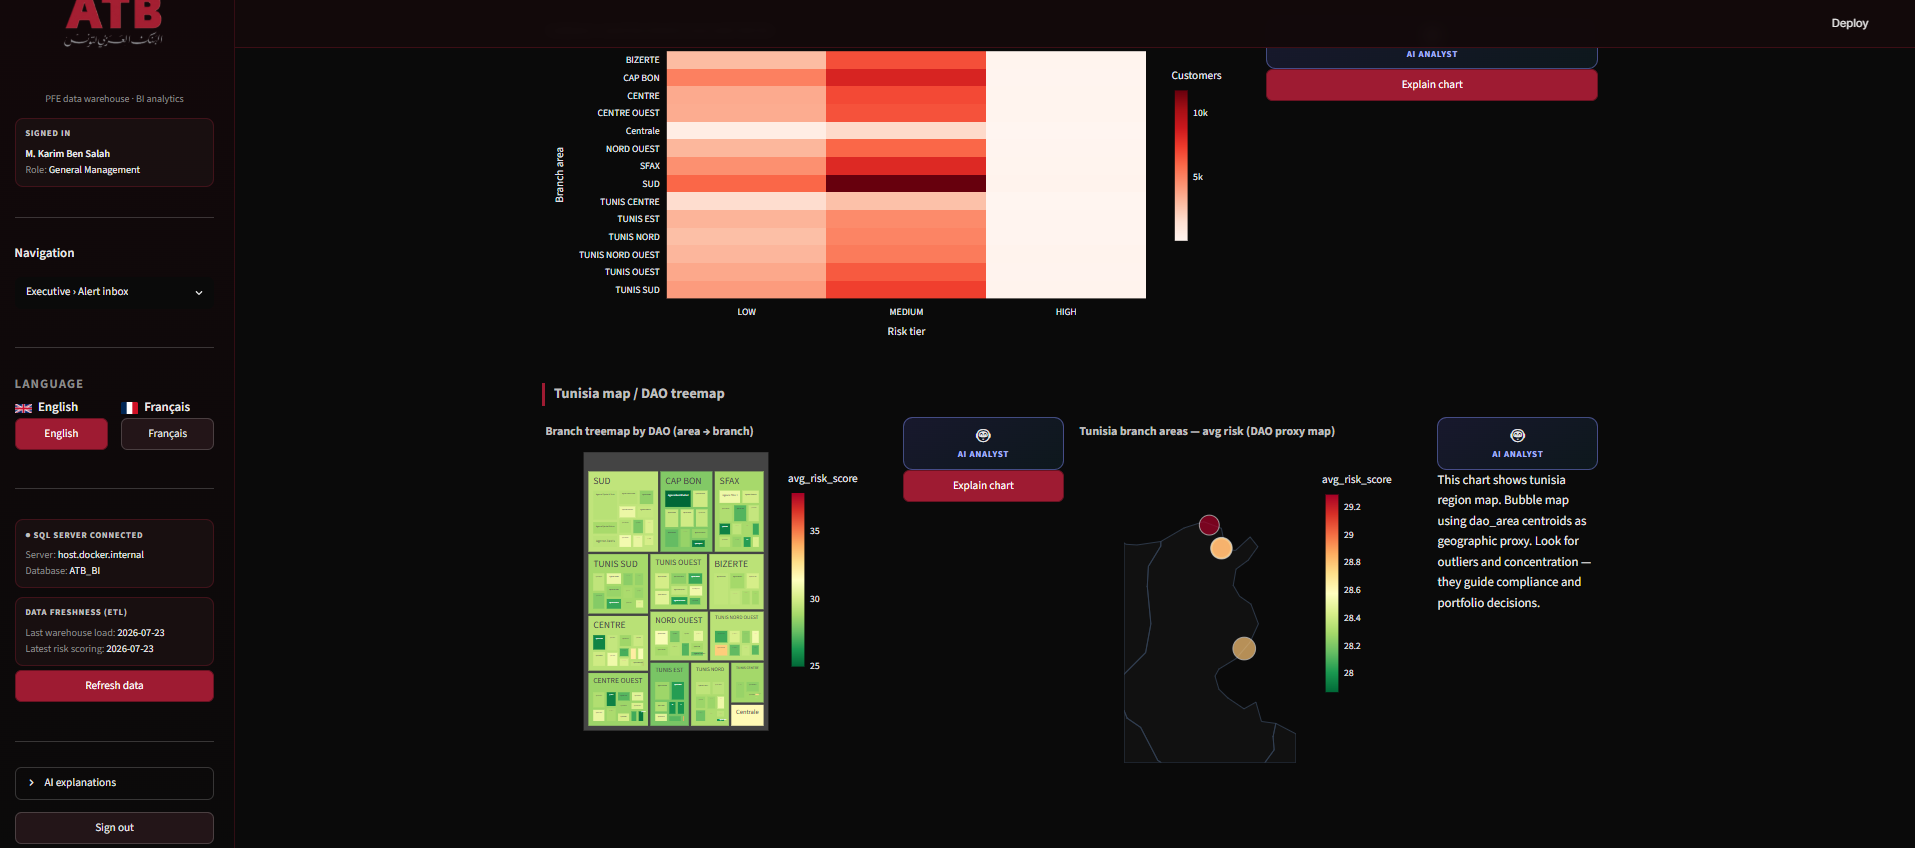
\includegraphics[width=0.95\textwidth]{figures/dash_ai_explain.png}
\caption{AI Analyst panel on-demand Gemini interpretation beside a dashboard chart}
\label{fig:gemini-ai-dashboard}
\end{figure}
\noindent Geographic risk charts (heatmap, DAO treemap, map)
each expose an Explain chart action; the response appears in the right-hand
panel without leaving the page.

\subsection{Integration with ML Outputs}

The same explanation mechanism extends to the \textbf{ML Risk Intelligence}
module, making quantitative model outputs accessible to non-technical
compliance staff:

\begin{itemize}
    \item On the \textbf{Curves \& SHAP} tab, the user can request an
          AI-generated interpretation of the probability score distribution.
          A typical response might read: ``The distribution shows that the
          vast majority of customers have a very low ML risk probability,
          consistent with the 1.3\% base rate. The right-hand tail of
          1{,}631 high-risk identifications represents the primary alert
          population that warrants compliance review.''
    \item On the \textbf{Batch \& alerts} tab, a natural-language agreement
          summary is generated on demand for example: ``The XGBoost model
          and the rules engine reach the same conclusion for 99.97\% of
          evaluated customers. The 34 remaining disagreements should be
          escalated for manual review by the compliance team.''
\end{itemize}

By combining on-demand AI narration with full user control over activation
and API credentials, the ATB BI platform establishes a responsible and
practical model of \textbf{human-in-the-loop AI governance}one where
artificial intelligence serves as a knowledgeable assistant rather than an
autonomous decision-maker.

%======================================================================
\section{Sprint 4 Summary CRISP-ML Deliverables}
\label{sec:sprint4_summary}
%======================================================================

\subsection{Deliverables by Phase}

\begin{table}[H]
\centering
\caption{Sprint~4 deliverables}
\label{tab:sprint4-deliverables-atb}
\begin{tabular}{|c|l|l|c|}
\hline
\textbf{Phase} & \textbf{Activity} & \textbf{Deliverable} & \textbf{Status} \\
\hline
1 & Business Understanding & Dual-layer rules + ML architecture & \checkmark \\
2 & Data Preparation & 5 notebooks, 34 features, SMOTETomek & \checkmark \\
3 & Model Engineering & 4 MLflow runs, XGBoost production & \checkmark \\
4 & Model Evaluation & ROC/PR, SHAP, overfitting report & \checkmark \\
5 & Deployment & ML Risk Intelligence + MLflow Registry pages & \checkmark \\
6 & Monitoring & Airflow DAGs, Docker, \texttt{PFE\_ML} scoring & \checkmark \\
\hline
\end{tabular}
\end{table}

\subsection{Production SLAs}

\begin{table}[H]
\centering
\caption{ML components in production}
\label{tab:sla-ml-production}
\begin{tabular}{|l|c|c|l|}
\hline
\textbf{Metric} & \textbf{Target} & \textbf{Result} & \textbf{Source} \\
\hline
Test F1 (XGBoost) & $\geq 0.70$ & \textbf{0.9545} & \texttt{training\_summary.json} \\
Test ROC-AUC & $\geq 0.80$ & \textbf{1.0000} & \texttt{training\_summary.json} \\
MLflow registry & Production stage & \textbf{OK} & \texttt{atb\_customer\_risk\_classifier} \\
Batch scoring table & Created & \textbf{OK} & \texttt{PFE\_ML.ml\_customer\_predictions} \\
Airflow ML DAG & Functional & \textbf{OK} & \texttt{dag\_ml\_pipeline} \\
Docker dashboard & Port 8501 & \textbf{OK} & \texttt{streamlit/Dockerfile} \\
\hline
\end{tabular}
\end{table}

%----------------------------------------------------------------------
% SCREENSHOT CHECKLIST (commented — capture these, copy to report/figures/, uncomment)
%----------------------------------------------------------------------
% ML RISK INTELLIGENCE (Streamlit ml_page.py)
%   [ ] ml_risk_intelligence_header.png   — page header + dual-layer banner + 5 tabs
%   [ ] ml_live_demo.png                  — Live demo: rules vs ML side-by-side cards
%   [ ] ml_batch_alerts.png               — Batch scoring KPIs + disagreement alert table
%   [ ] ml_curves_shap_tab.png            — ROC/PR curves + confusion matrix + SHAP
%   [ ] ml_xgboost_metrics_tab.png        — Metrics KPIs + bar charts + output gallery
%
% MLFLOW REGISTRY (Streamlit mlflow_page.py)
%   [ ] mlflow_registry_page.png          — Production card + registered models + runs
%
% JUPYTER / TRAINING OUTPUTS (copy from 4_ml/outputs/)
%   [ ] eda_target_and_distribution.png
%   [ ] eda_correlation_heatmap.png
%   [ ] 03_model_comparison_bars.png
%   [ ] 05_test_metrics_comparison.png
%   [ ] 05_roc_pr_curves.png
%   [ ] shap_local_waterfall.png
%   [ ] mlflow_dashboard.png              — optional: native MLflow UI
%
% OPS / INFRASTRUCTURE
%   [ ] airflow_ml_dag.png                — dag_ml_pipeline graph view
%   [ ] streamlit_docker_running.png
%   [ ] ssms_pfe_ml_predictions.png
%----------------------------------------------------------------------

%======================================================================
\section{Conclusion}
\label{sec:release3_conclusion}
%======================================================================

Release~3 closes the platform with a supervised learning layer aligned to CRISP-ML.
Four classifiers were compared under identical warehouse features and temporal
holdout; XGBoost was selected as the production model (test F1 $= 0.9545$,
ROC-AUC $= 1.0$) and registered in MLflow. The rules-based global risk score remains
the official auditable measure, while ML acts as a screening assistant that raises
disagreement alerts and supports what-if analysis in Streamlit.

SHAP explanations, Airflow retraining and batch scoring into \texttt{PFE\_ML} make the
model operable for compliance and risk teams without replacing the deterministic
engine. Sprint~4 therefore delivers predictive capability that is reproducible,
explainable and integrated into the same dashboard already used for BI steering.


\chapter*{General Conclusion and Perspectives}
\label{chap:conclusion}
\markboth{\MakeUppercase{General Conclusion and Perspectives}}{}%
\addcontentsline{toc}{chapter}{General Conclusion and Perspectives}
\vspace{0.5cm}

This project started from a simple observation: decision-makers at Arab Tunisian Bank
did not have a reliable, shared view of their customer portfolio. By the end of
this work, that gap was filled --- with a platform that centralises data, produces
visual dashboards, and adds a layer of predictive intelligence to support risk decisions.

The project was delivered in three successive phases. The first secured the environment
and put automated pipelines in place. The second built the analytical foundation ---
a structured data warehouse feeding role-based dashboards for branch managers,
compliance officers, and general management. The third introduced a machine learning
model that flags high-risk customers and explains its reasoning in plain terms,
always alongside the official rules-based score.

The main contribution goes beyond the technical side. What was built is a single,
trustworthy source of information that different teams can rely on together ---
something the bank did not have before.

Looking ahead, several directions are worth exploring. On the modelling side, regular
monitoring and periodic retraining would help the system stay accurate over time.
On the data side, the most promising evolution is the move toward real-time data
streaming --- replacing the current nightly batch approach with a live data flow,
so that risk indicators and dashboards reflect what is happening at the bank right now,
not yesterday. This shift would significantly strengthen the platform's value for
time-sensitive compliance and credit decisions.

More broadly, this project shows that a well-structured engineering effort, even at
graduation project scale, can lay a solid foundation for a modern, data-driven banking
operation.


\newpage
\appendix
\addcontentsline{toc}{chapter}{Annexes}
%\markboth{\MakeUppercase{Annexe}}{}





%%%%%%%%%%%%%%%%%%%%%%%%%%%%%%%%%%%%%%%%%%%%%%%%%%%%
% Bibliography — only cited references (no \nocite{*})
%%%%%%%%%%%%%%%%%%%%%%%%%%%%%%%%%%%%%%%%%%%%%%%%%%%%

%\bibliographystyle{apalike}
\bibliographystyle{plain}
\renewcommand{\bibname}{References}
\bibliography{Biblio.bib}

\cleardoublepage

%%%%%%%%%%%%%%%%%%%%%%%%%%%%%%%%%%%%%%%%%%%%%%%%%%%%
% Webography
%%%%%%%%%%%%%%%%%%%%%%%%%%%%%%%%%%%%%%%%%%%%%%%%%%%%
\chapter*{Webography}
\markboth{\MakeUppercase{Webography}}{}%
\addcontentsline{toc}{chapter}{Webography}

The following online resources were consulted during the design and implementation of the
platform (official documentation and technical references).

\begin{itemize}
    \item \textbf{Apache Airflow} --- workflow orchestration documentation.\\
          \url{https://airflow.apache.org/docs/}
    \item \textbf{Airbyte} --- open-source data integration platform.\\
          \url{https://docs.airbyte.com/}
    \item \textbf{dbt (data build tool)} --- transformation and testing documentation.\\
          \url{https://docs.getdbt.com/}
    \item \textbf{Streamlit} --- Python dashboard framework.\\
          \url{https://docs.streamlit.io/}
    \item \textbf{MLflow} --- experiment tracking and model registry.\\
          \url{https://mlflow.org/docs/latest/index.html}
    \item \textbf{XGBoost} --- gradient boosting library documentation.\\
          \url{https://xgboost.readthedocs.io/}
    \item \textbf{scikit-learn} --- machine learning toolbox.\\
          \url{https://scikit-learn.org/stable/}
    \item \textbf{SHAP} --- model explainability (SHapley Additive exPlanations).\\
          \url{https://shap.readthedocs.io/}
    \item \textbf{Plotly} --- interactive charting library used in Streamlit.\\
          \url{https://plotly.com/python/}
    \item \textbf{Docker} --- container platform documentation.\\
          \url{https://docs.docker.com/}
    \item \textbf{Microsoft SQL Server} --- database engine documentation.\\
          \url{https://learn.microsoft.com/en-us/sql/sql-server/}
    \item \textbf{SQLAlchemy} --- Python SQL toolkit and ORM.\\
          \url{https://docs.sqlalchemy.org/}
    \item \textbf{Google Gemini API} --- generative AI for chart explanations.\\
          \url{https://ai.google.dev/gemini-api/docs}
    \item \textbf{Scrum Guide} --- agile delivery framework.\\
          \url{https://scrumguides.org/}
    \item \textbf{CRISP-ML(Q)} --- machine learning process with quality assurance
          (Studer et al.).\\
          \url{https://arxiv.org/abs/2003.05155}
    \item \textbf{Draw.io (diagrams.net)} --- architecture and UML diagrams.\\
          \url{https://www.diagrams.net/}
    \item \textbf{Arab Tunisian Bank} --- institutional website.\\
          \url{https://www.atb.tn/}
\end{itemize}

\cleardoublepage%


\printindex

\end{document}
